% !TEX root = ../Elements.tex
% Greek and English text last checked 13/03/2013
%%%%%%
% BOOK 1
%%%%%%
\pdfbookmark[0]{Book 1}{book1}
\pagestyle{empty}
\begin{center}
{\Huge ELEMENTS BOOK 1}\\
\spa\spa\spa
{\huge\it Fundamentals of Plane Geometry Involving}\\[0.5ex] {\huge\it 
Straight-Lines}
\end{center}
%\vspace{2cm}
%% Removed epsf size command
%\centerline{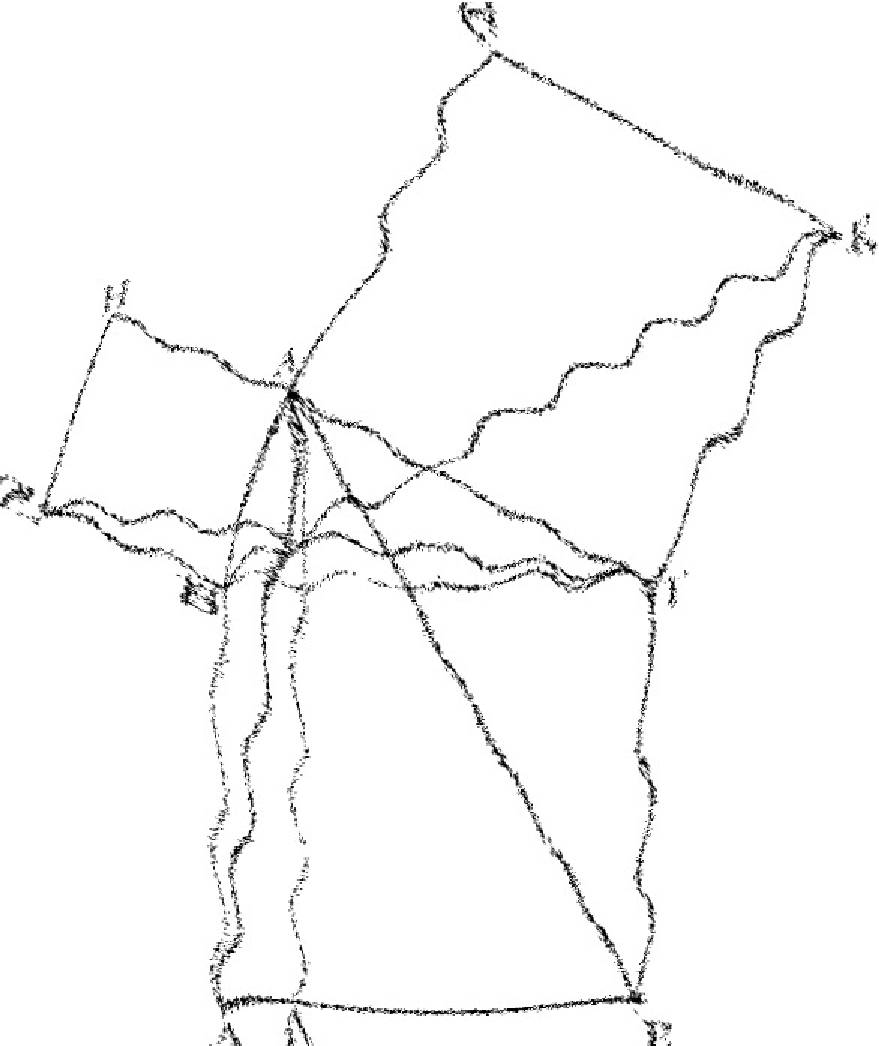
\includegraphics[width=0.8\textwidth]{Book01/front.pdf}}
\newpage

%%%%%%%
% Definitions
%%%%%%%
\pdfbookmark[1]{Definitions}{def1}
\pagestyle{fancy}
\cfoot{\gr{ }}
\lhead{\large\gr{ΣΤΟΙΘΕΙΩΝ  {1}.}}
\rhead{\large ELEMENTS BOOK 1}
\begin{Parallel}{}{} 
\ParallelLText{
\begin{center}
\large{\gr{ὍΟροι}.}
\end{center}
\vspace*{-7pt}

\ggn{1}.~\gr{Σημεῖόν ἐστιν, οὗ μέρος οὐθέν.}

\ggn{2}.~\gr{Γραμμὴ δὲ μῆκος ἀπλατές.}

\ggn{3}.~\gr{Γραμμῆς δὲ πέρατα σημεῖα.}

\ggn{4}.~\gr{Εὐθεῖα γραμμή ἐστιν, ἥτις ἐξ ἴσου τοῖς ἐφ'
ἑαυτῆς σημείοις κεῖται.}

\ggn{5}.~\gr{Ἐπιφάνεια δέ ἐστιν, ὃ μῆκος καὶ πλάτος μόνον ἔχει.}

\ggn{6}.~\gr{Ἐπιφανείας δὲ πέρατα  γραμμαί.}

\ggn{7}.~\gr{Ἐπίπεδος ἐπιφάνειά ἐστιν, ἥτις ἐξ ἴσου
ταῖς ἐφ' ἑαυτῆς εὐθείαις κεῖται.}

\ggn{8}.~\gr{Ἐπίπεδος δὲ γωνία ἐστὶν ἡ ἐν ἐπιπέδῳ δύο γραμμῶν
ἁπτομένων ἀλλήλων καὶ μὴ ἐπ' εὐθείας κειμένων πρὸς
ἀλλήλας τῶν γραμμῶν κλίσις.}

\ggn{9}.~\gr{ὍΟταν δὲ αἱ περιέθουσαι τὴν γωνίαν γραμμαὶ εὐθεῖαι ὦσιν, εὐθύγραμμος καλεῖται ἡ γωνία.}

\ggn{10}.~\gr{ὍΟταν δὲ εὐθεῖα ἐπ' εὐθεῖαν σταθεῖσα τὰξ ἐφεχῆς γωνίας ἴσας ἀλλήλαις ποιῆ|, ὀρθὴ ἑκατέρα τῶνὸίσων γωνιῶν
ἐστι, καὶ ἡ ἐφεστηκυῖα εὐθεῖα κάθετος καλεῖται, ἐφ' ἣν ἐφέστηκεν.}

\ggn{11}.~\gr{Ἀμβλεῖα γωνία ἐστὶν ἡ μείζων ὀρθῆς.}

\ggn{12}.~\gr{Ὀξεῖα δὲ ἡ ἐλάσσων ὀρθῆς.}

\ggn{13}.~\gr{ὍΟρος ἐστίν, ὅ τινόξ ἐστι πέρας.}

\ggn{14}.~\gr{Σχῆμά ἐστι τὸ ὑπό τινος ἢ τινων ὅρων περιεχόμενον.}

\ggn{15}.~\gr{Κύκλος ἐστὶ σχῆμα ἐπίπεδον ὑπὸ μιᾶς γραμμῆς περιεχόμενον [ἣ καλεῖται περιφέρεια], πρὸς ἣν ἀφ' ἑνὸς σημείου
τῶν ἐντὸς τοῦ σχήματος κειμένων πᾶσαι αἱ προσπίπτουσαι εὐθεῖαι
[πρὸς τὴν τοῦ κύκλου περιφέρειαν]  ἴσαι ἀλλήλαις εἰσίν.}

\ggn{16}.~\gr{Κέντρον δὲ τοῦ κύκλου τὸ σημεῖον καλεῖται.}

\ggn{17}.~\gr{Διάμετρος δὲ τοῦ κύκλου ἐστὶν εὐθεῖά τις διὰ τοῦ κέντρου
ἠγμένη καὶ περατουμένη ἐφ' ἑκάτερα τὰ μέρη ὑπὸ τῆς τοῦ κύκλου περιφερείας, ἥτις καὶ δίθα τέμνει τὸν κύκλον.}

\ggn{18}.~\gr{Ἡμικύκλιον δέ ἐστι τὸ περιεχόμενον σχῆμα ὑπό τε τῆς διαμέτρου καὶ τῆς ἀπολαμβανομένης ὑπὸ αὐτῆς περιφερείας. κέντρον δὲ τοῦ ἡμικυκλίου τὸ αὐτό, ὃ καὶ τοῦ κύκλου ἐστίν.}

\ggn{19}.~\gr{Σθήματα εὐθύγραμμά ἐστι τὰ ὑπὸ εὐθειῶν περιεχόμενα,
τρίπλευρα μὲν τὰ ὑπὸ τριῶν, τετράπλευρα
δὲ τὰ ὑπὸ τεσσάρων, πολύπλευρα δὲ τὰ ὑπὸ πλειόνωνὸὴ τεσσάρων
εὐθειῶν περιεχόμενα.}

\ggn{20}.~\gr{Τῶν δὲ τριπλεύρων σχημάτων ἰσόπλευρον μὲν τρίγωνόν ἐστι τὸ
τὰξ τρεῖς ἴσας ἔχον πλευράς, ἰσοσκελὲξ δὲ τὸ τὰξ δύο μόνας ἴσας ἔχον πλευράς, σκαληνὸν δὲ τὸ τὰξ τρεῖς ἀνίσους ἔχον πλευράς.}

\ggn{21}~\gr{ὸ'Ετι δὲ τῶν τριπλεύρων σχημάτων ὀρθογώνιον μὲν τρίγωνόν ἐστι τὸ  ἔχον ὀρθὴν γωνίαν,  ἀμβλυγώνιον δὲ τὸ  ἔχον ἀμβλεῖαν
γωνίαν, ὀξυγώνιον δὲ τὸ τὰξ τρεῖς ὀξείας ἔχον γωνίας.}

\ggn{22}.~\gr{Τὼν δὲ τετραπλεύρων σχημάτων τετράγωνον μέν ἐστιν, ὃ 
ἰσόπλευρόν τέ ἐστι καὶ ὀρθογώνιον, ἑτερόμ  ηκες δέ, ὃ
ὀρθογώνιον μέν, οὐκ ἰσόπλευρον δέ, ῥόμβος δέ, ὃ ἰσόπλευρον
μέν, οὐκ
ὀρθογώνιον δέ, ὁρομβοειδὲξ δὲ τὸ τὰξ ἀπεναντίον πλευράς τε καὶ γωνίας ἴσας ἀλλήλαις ἔχον, ὃ οοὔτε
ἰσόπλευρόν ἐστιν οοὔτε ὀρθογώνιον; τὰ δὲ παρὰ ταῦτα τετράπλευρα
τραπέζια καλείσθω.}

\ggn{23}.~\gr{Παράλληλοί εἰσιν εὐθεῖαι, αὁίτινες ἐν τῷ αὐτῷ ἐπιπέδῳ
οὸῦσαι καὶ ἐκβαλλόμεναι εἰξ ἄπειρον ἐφ' ἑκάτερα τὰ μέρη
ἐπὶ μ  ηδέτερα  συμπίπτουσιν ἀλλήλαις.}}

\ParallelRText{
\begin{center}
{\large Definitions}
\end{center}

1.~A point is that of which there is no part.

2.~And a line is a length without breadth.

3.~And the extremities of a line are points.

4.~A straight-line is (any) one which lies  evenly with points on itself.

5.~And a surface is that which has length and breadth only.

6.~And the extremities of a surface are lines.

7.~A plane surface is (any) one which lies evenly with the straight-lines on itself.

8.~And a plane angle is the inclination of the lines to one another, when two lines in a plane 
meet one another, and are not lying in a straight-line.

9.~And when the lines containing the angle are straight then the angle is called rectilinear.

10.~And when a straight-line stood upon (another) straight-line makes adjacent angles (which are) equal to one another, each of the equal angles is a
right-angle, and the former straight-line  is called a perpendicular to that upon which it stands.

11.~An obtuse angle is one greater than a right-angle.

12.~And an acute angle (is) one less than a right-angle.

13.~A boundary is that which is the extremity of something.

14.~A figure is that which is contained by some boundary or boundaries.

15.~A circle is a plane figure  contained by a single line [which is called a circumference], (such that) all of the straight-lines  radiating towards
 [the circumference] from one
point amongst those lying inside the figure  are equal to one another.

16.~And the point is called the center of the circle.

17.~And a diameter of the circle is any straight-line, being drawn through the
center, and terminated in each direction by the circumference of the circle. (And) any such (straight-line) also cuts the circle in half.$^\dag$

18.~And a semi-circle is the figure contained by the diameter  and
the circumference  cut off by it. And the center of the semi-circle is the same (point)
as (the center of) the circle.

19.~Rectilinear figures are those (figures) contained by straight-lines: trilateral
figures being those contained by three straight-lines,  quadrilateral   by four,
and multilateral by more than four.

20.~And of the trilateral figures: an equilateral triangle is that having
three equal sides, an isosceles (triangle) that having only two equal sides,
and a scalene (triangle) that having three unequal sides.

21.~And further of the trilateral figures: a right-angled triangle is that having
a right-angle, an obtuse-angled  (triangle) that having an obtuse
angle, and an acute-angled (triangle) that having three acute angles.

22.~And of the quadrilateral figures: a square is that which is right-angled
and equilateral, a rectangle that which is right-angled but not equilateral,
a rhombus that which is equilateral but not right-angled, and a rhomboid that
having opposite sides and angles equal to one another which is neither
right-angled nor equilateral. And let quadrilateral figures besides these be called
trapezia.

23.~Parallel lines are straight-lines which, being in the same plane, and
being produced to infinity in each direction, meet with one another in
neither (of these directions).}
\end{Parallel}
{\footnotesize 
\noindent $^\dag$ This should really be counted as a postulate, rather than as part of a definition.}

%%%%%%
% Postulates
%%%%%%
\begin{Parallel}{}{} 
\ParallelLText{
\begin{center}
{\large \gr{Αἰτήματα.}}
\end{center}\vspace*{-7pt}

\ggn{1}.~\gr{Ἠιτήσθω ἀπὸ παντὸς σημείου ἐπὶ πᾶν σημεῖον εὐθεῖαν
γραμμὴν ἀγαγεῖν.}

\ggn{2}.~\gr{Καὶ πεπερασμένην εὐθεῖαν κατὰ τὸ συνεθὲξ ἐπ' εὐθείας ἐκβαλεῖν.}

\ggn{3}.~\gr{Καὶ παντὶ κέντρῳ καὶ διαστήματι κύκλον γράφεσθαι.}

\ggn{4}.~\gr{Καὶ πάσας τὰξ ὀρθὰξ γωνίας ἴσας ἀλλήλαις εὸῖναι.}

\ggn{5}.~\gr{Καὶ ἒαν εἰξ δύο εὐθείας εὐθεῖα ἐμπίπτουσα τὰξ ἐντὸς
καὶ ἐπὶ τὰ αὐτὰ μέρη γωνίας δύο ὀρθῶν ἐλάσσονας ποιῆ|,
ἐκβαλλομένας τὰξ δύο εὐθείας ἐπ'  ἄπειρον συμπίπτειν, ἐφ' ὁὰ
μέρη εἰσὶν αἱ τῶν δύο ὀρθῶν ἐλάσσονες.}}

\ParallelRText{
\begin{center}
{\large Postulates}
\end{center}

1.~Let it be postulated$^\dag$ (that it is possible) to draw a straight-line from any point to any point;

2.~And to produce a finite straight-line continuously in a straight-line;

3.~And to draw a circle with any center and radius.

4.~And that all right-angles are equal to one another.

5.~And that if a straight-line falling across two (other) straight-lines makes 
internal angles on the same side (of itself whose sum is) less than two right-angles, (then) the two (other) straight-lines, being produced to infinity, meet on that side (of the original straight-line) that the (sum of the internal angles) is less
than two right-angles (and do not meet on the other side).$^\ddag$}
\end{Parallel}
{\footnotesize
\noindent $^\dag$ Literally, "let it have been postulated". 
The Greek present perfect tense indicates a past action with present
significance. Hence, the 3rd-person present perfect imperative \gr{ἠιτήσθω} means  ``let it be postulated" in the sense ``let it stand as postulated", but not  ``let the
postulate be now brought forward". This peculiar Greek idiom is used throughout the Elements.\\
\noindent $^\ddag$ This postulate effectively specifies that we are dealing with the geometry of
flat, rather than  curved, space.}

%%%%%%%%%%
% Common Notions
%%%%%%%%%%
\begin{Parallel}{}{} 
\ParallelLText{
\begin{center}
{\large \gr{Κοιναὶ ὸέννοιαι.}}
\end{center}\vspace*{-7pt}

\ggn{1}.~\gr{Τὰ τῷ αὐτῷ  ἴσα καὶ ἀλλήλοις ἐστὶν ἴσα.}

\ggn{2}.~\gr{Καὶ ἒανὸίσοις ἴσα προστεθῆ|, τὰ ὅλα ἐστὶν ἴσα.}

\ggn{3}.~\gr{Καὶ ἒαν ἀπὸ ὸίσων ἴσα ἀφαιρεθῆ|, τὰ καταλειπόμενά ἐστιν ἴσα.}

\ggn{4}.~\gr{Καὶ τὰ ἐφαρμόζοντα ἐπ' ἀλλήλα ἴσα ἀλλήλοις ἐστίν.}

\ggn{5}.~\gr{Καὶ τὸ ὅλον τοῦ μέρους μεῖζόν [ἐστιν].}}

\ParallelRText{
\begin{center}
{\large Common Notions}
\end{center}

1.~Things equal to the same thing are also equal to one another.

2.~And  if equal things are added to equal things (then) the wholes are equal.

3.~And if equal things are subtracted from equal things (then) the remainders are
equal.$^\dag$

4.~And things coinciding with one another are equal to one another.

5.~And the whole [is] greater than the part.}
\end{Parallel}
{\footnotesize
\noindent $^\dag$ As an obvious extension of C.N.s~2 \& 3---if equal things
are added or subtracted from the two sides of an inequality then  the inequality
remains an inequality of the same type.}\\~\\

%%%%%%
% Prop 1.1
%%%%%%
\pdfbookmark[1]{Proposition 1.1}{prop1.1}
\begin{Parallel}{}{} 
\ParallelLText{
\begin{center}
{\large \ggn{1}.}
\end{center}\vspace*{-7pt}

\gr{Ἐπὶ τῆς δοθείσης εὐθείας πεπερασμένης τρίγωνον ἰσόπλευρον συστήσασθαι.}

\gr{Ἔστω ἡ δοθεῖσα εὐθεῖα πεπερασμένη ἡ ΑΒ.}

\gr{Δεῖ δὴ ἐπὶ τῆς ΑΒ εὐθείας τρίγωνον ἰσόπλευρον συστήσνασθαι.}

% Removed epsf size command
\centerline{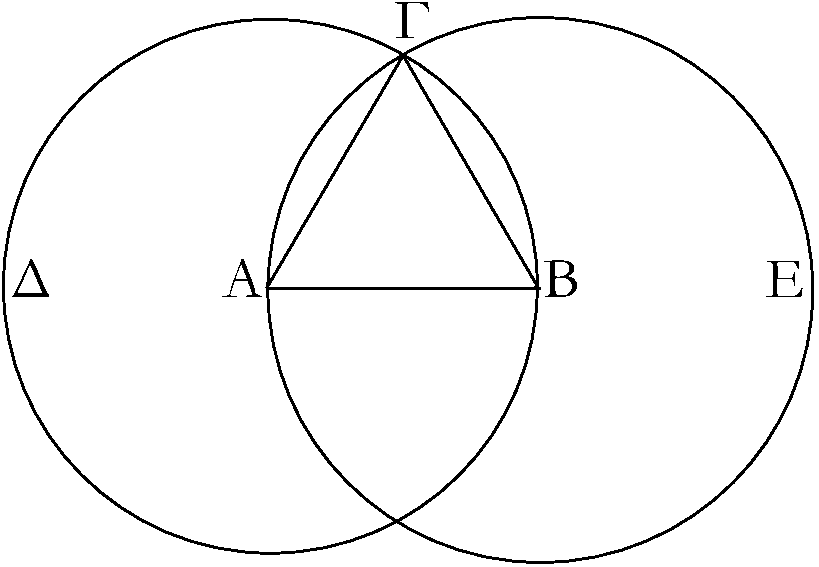
\includegraphics[width=0.8\textwidth]{Book01/fig01g.pdf}}

\gr{Κέντρῳ μὲν τῷ Α διαστήματι δὲ τῷ ΑΒ κύκλος γεγράφθω ὁ ΒΓΔ,
καὶ πάλιν κέντρῳ μὲν τῷ Β διαστήματι δὲ τῷ ΒΑ κύκλος γεγράφθω
ὁ ΑΓΕ, καὶ ἀπὸ τοῦ Γ σημείου, καθὸ ὃ τέμνουσιν ἀλλήλους οἱ
κύκλοι, ἐπί τὰ Α, Β σημεῖα ἐπεζεύθθωσαν εὐθεῖαι αἱ ΓΑ, ΓΒ.}

\gr{Καὶ ἐπεὶ τὸ Α σημεῖον κέντρον ἐστὶ τοῦ ΓΔΒ κύκλου, ὸίση ἐστὶν
ἡ ΑΓ τῇ ΑΒ; πάλιν, ἐπεὶ τὸ Β σημεῖον κέντρον ἐστὶ τοῦ ΓΑΕ
κύκλου, ὸίση ἐστὶν ἡ ΒΓ τῇ ΒΑ. ἐδείθθη δὲ καὶ ἡ ΓΑ τῇ  ΑΒὸίση;
ἑκατέρα ἄρα τῶν ΓΑ, ΓΒ τῇ ΑΒ ἐστινὸίση. τὰ δὲ τῷ αὐτῷ
 ἴσα καὶ ἀλλήλοις ἐστὶν ἴσα;  καὶ ἡ ΓΑ ἄρα τῇ ΓΒ ἐστινὸίση;
αἱ τρεῖς ἄρα αἱ ΓΑ, ΑΒ, ΒΓ ἴσαι ἀλλήλαις εἰσίν.}

\gr{Ἰσόπλευρον ἄρα ἐστὶ τὸ ΑΒΓ τρίγωνον. καὶ συνέσταται ἐπὶ
τῆς δοθείσης εὐθείας πεπερασμένης τῆς ΑΒ. ὅπερ ἔδει ποιῆσαι.}}

\ParallelRText{
\begin{center}
{\large Proposition 1}
\end{center}
To construct an equilateral triangle on a given finite straight-line.

Let $AB$ be the given finite straight-line.

So it is required to construct an equilateral triangle on the straight-line $AB$.

% Removed epsf size command
\centerline{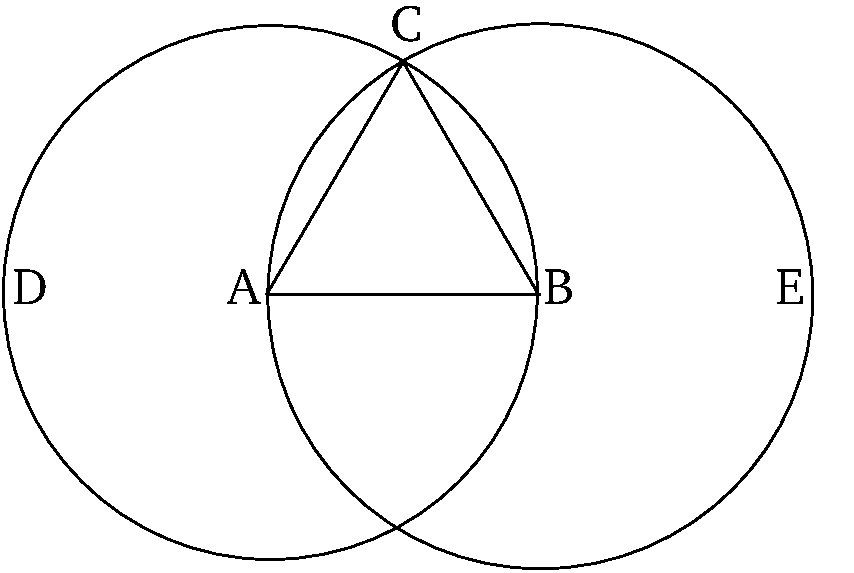
\includegraphics[width=0.8\textwidth]{Book01/fig01e.pdf}}

Let the circle $BCD$ with center $A$ and radius $AB$ be drawn$^\dag$ [Post.~3], and again
let the circle $ACE$ with center $B$ and radius $BA$ be drawn [Post.~3].
And let the straight-lines $CA$ and $CB$ be joined from the point $C$, where the circles cut one another,$^\ddag$ to the points $A$ and $B$ (respectively) [Post.~1].

And since the point $A$ is the center of the circle $CDB$, $AC$ is equal to $AB$ [Def.~1.15]. Again,
since the point $B$ is the center of the circle $CAE$, $BC$ is equal to $BA$ [Def.~1.15]. But $CA$ 
was also shown (to be) equal to $AB$. Thus, $CA$ and $CB$ are each equal to $AB$. But things equal to the same thing are also equal to one another [C.N.~1]. Thus, $CA$ is also equal to $CB$. Thus, the three (straight-lines) $CA$, $AB$, and $BC$ are equal to one another.

Thus, the triangle $ABC$ is equilateral, and has been constructed on the
given finite straight-line $AB$. (Which is) the very thing it was required to do.}
\end{Parallel}
{\footnotesize
\noindent $^\dag$ Literally, "have been drawn". The use of this peculiar Greek idiom will pass
without further comment.\\
\noindent $^\ddag$ The assumption that the circles do indeed cut one another should be counted as an additional 
postulate. There is also an implicit assumption that two straight-lines cannot share a common segment.}

%%%%%%
% Prop 1.2
%%%%%%
\pdfbookmark[1]{Proposition 1.2}{pdf1.2}
\begin{Parallel}{}{} 
\ParallelLText{
\begin{center}
{\large \ggn{2}.}
\end{center}\vspace*{-7pt}

\gr{Πρὸξ τῷ δοθέντι σημείῳ τῇ δοθείσῃ εὐθείᾳ  ἴσην εὐθεῖαν θέσθαι.}

\gr{Ἔστω τὸ μὲν δοθὲν σημεῖον τὸ Α, ἡ δὲ δοθεῖσα εὐθεῖα ἡ ΒΓ;
δεῖ δὴ πρὸς τῷ Α σημείῳ τῇ δοθείσῃ εὐθείᾳ τῇ ΒΓ ἴσην εὐθεῖαν θέσθαι.}

\gr{Ἐπεζεύθθω γὰρ ἀπὸ τοῦ Α σημείου ἐπί τὸ Β σημεῖον εὐθεῖα
ἡ ΑΒ, καὶ συνεστάτω ἐπ' αὐτῆς τρίγωνον ἰσόπλευρον τὸ ΔΑΒ, καὶ
ἐκβεβλήσθωσαν ἐπ' εὐθείας ταῖς  ΔΑ, ΔΒ εὐθεῖαι αἱ ΑΕ, ΒΖ, καὶ
κέντρῳ μὲν τῷ Β διαστήματι δὲ τῷ ΒΓ κύκλος γεγράφθω ὁ
ΓΗΘ, καὶ πάλιν κέντρῳ τῷ Δ καὶ διαστήματι τῷ ΔΗ κύκλος γεγράφθω ὁ
ΗΚΛ.}\\

% Removed epsf size command
\centerline{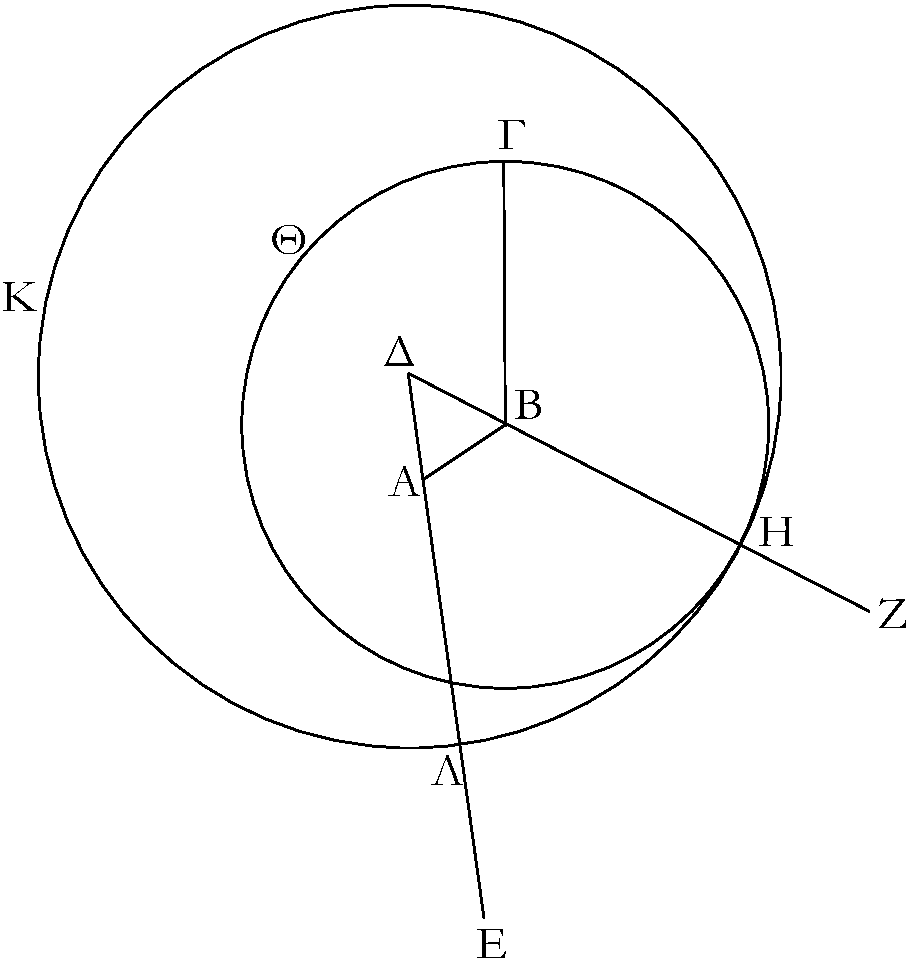
\includegraphics[width=0.8\textwidth]{Book01/fig02g.pdf}}

\gr{Ἐπεὶ οὸῦν τὸ Β σημεῖον κέντρον ἐστὶ τοῦ ΓΗΘ, ὸίση ἐστὶν
ἡ ΒΓ τῇ ΒΗ. πάλιν, ἐπεὶ τὸ Δ σημεῖον κέντρον ἐστὶ τοῦ
ΗΚΛ κύκλου, ὸίση ἐστὶν ἡ ΔΛ τῇ ΔΗ, ὁῶν ἡ ΔΑ τῇ ΔΒὸίση ἐστίν.
λοιπὴ  ἄρα ἡ ΑΛ λοιπῆ| τῇ ΒΗ ἐστινὸίση. 
ἐδείθθη δὲ καὶ ἡ ΒΓ τῇ ΒΗὸίση;
ἑκατέρα ἄρα τῶν ΑΛ, ΒΓ
τῇ ΒΗ ἐστινὸίση. τὰ δὲ τῷ αὐτῷ  ἴσα καὶ ἀλλήλοις ἐστὶν ἴσα; καὶ ἡ ΑΛ ἄρα τῇ ΒΓ ἐστινὸίση.}

\gr{Πρὸξ ἄρα τῷ δοθέντι σημείῳ τῷ Α τῇ δοθείσῃ εὐθείᾳ τῇ ΒΓὸίση εὐθεῖα κεῖται ἡ ΑΛ; ὅπερ ἔδει ποιῆσαι.}}

\ParallelRText{
\begin{center}
{\large Proposition 2$^\dag$}
\end{center}

To place a straight-line equal to a given straight-line at a given point (as an extremity).

Let $A$ be the given point, and $BC$ the given straight-line. So  it is required to
place a straight-line at point $A$ equal to the given straight-line $BC$.

For  let the straight-line $AB$ be joined from point $A$ to point $B$ [Post.~1], and let the
equilateral triangle $DAB$ be  constructed upon it [Prop.~1.1].  And let the
straight-lines $AE$ and $BF$ be produced in a straight-line with $DA$ and $DB$  (respectively) [Post.~2].
And let the circle $CGH$ with center $B$ and radius $BC$ be drawn
[Post.~3], and again let the circle $GKL$ with center $D$ and radius $DG$ be drawn [Post.~3].

% Removed epsf size command
\centerline{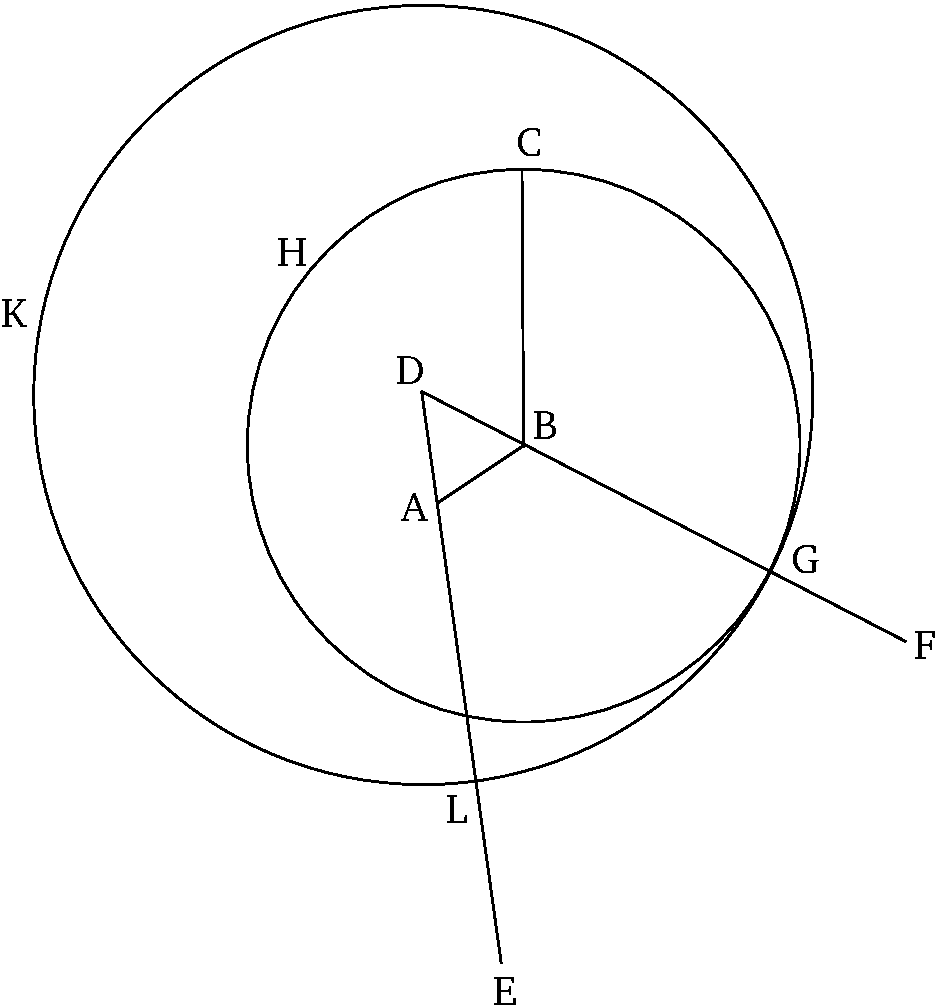
\includegraphics[width=0.8\textwidth]{Book01/fig02e.pdf}}

Therefore, since the point $B$ is the center of (the circle) $CGH$, $BC$ is equal to 
$BG$ [Def.~1.15]. Again, since the point $D$ is the center of the circle $GKL$, $DL$ is equal to $DG$ [Def.~1.15]. And within these,  $DA$ is equal to $DB$. Thus, the remainder $AL$ is equal to the remainder $BG$ [C.N.~3]. But $BC$ was also shown (to be)  equal to $BG$. Thus,  $AL$
and $BC$ are each equal to $BG$. But things equal to the same thing are also equal to one another [C.N.~1]. Thus, $AL$ is also equal to $BC$.

Thus, the straight-line $AL$, equal to the given straight-line $BC$,
has been placed at the given point $A$. (Which is) the very thing it was required to do.}
\end{Parallel}
{\footnotesize
\noindent $^\dag$ This proposition admits of a number
of different cases, depending on the relative positions of the point $A$
and the line $BC$. In such situations, Euclid invariably only considers one
particular case---usually, the most difficult---and leaves the remaining cases as
exercises for the reader.}

%%%%%%
% Prop 1.3
%%%%%%
\pdfbookmark[1]{Proposition 1.3}{pdf1.3}
\begin{Parallel}{}{} 
\ParallelLText{
\begin{center}
{\large \ggn{3}.}
\end{center}\vspace*{-7pt}

\gr{Δύο δοθεισῶν εὐθειῶν ἀνίσων ἀπὸ τῆς μείζονος τῇ ἐλάσσονι ἴσην εὐθεῖαν ἀφελεῖν.}

\gr{Ἔστωσαν αἱ δοθεῖσαι δύο εὐθεῖαιὸάνισοι αἱ ΑΒ, Γ, ὁῶν μείζωνὸέστω ἡ ΑΒ; δεῖ δὴ ἀπὸ τῆς μείζονος τῆς ΑΒ τῇ ἐλάσσονι τῇ Γ ἴσην εὐθεῖαν ἀφελεῖν.}

\gr{Κείσθω πρὸς τῷ Α σημείῳ τῇ Γ εὐθείᾳ ὸίση ἡ ΑΔ; καὶ κέντρῳ μὲν τῷ Α διαστήματι δὲ τῷ ΑΔ κύκλος γεγράφθω ὁ ΔΕΖ.}

\gr{Καὶ ἐπεὶ τὸ Α σημεῖον κέντρον ἐστὶ τοῦ ΔΕΖ κύκλου, ὸίση ἐστὶν ἡ ΑΕ τῇ ΑΔ; ἀλλὰ καὶ ἡ Γ τῇ ΑΔ ἐστινὸίση. ἑκατέρα ἄρα τῶν ΑΕ, Γ τῇ ΑΔ ἐστινὸίση; ὁώστε καὶ ἡ ΑΕ τῇ Γ ἐστινὸίση.}

% Removed epsf size command
\centerline{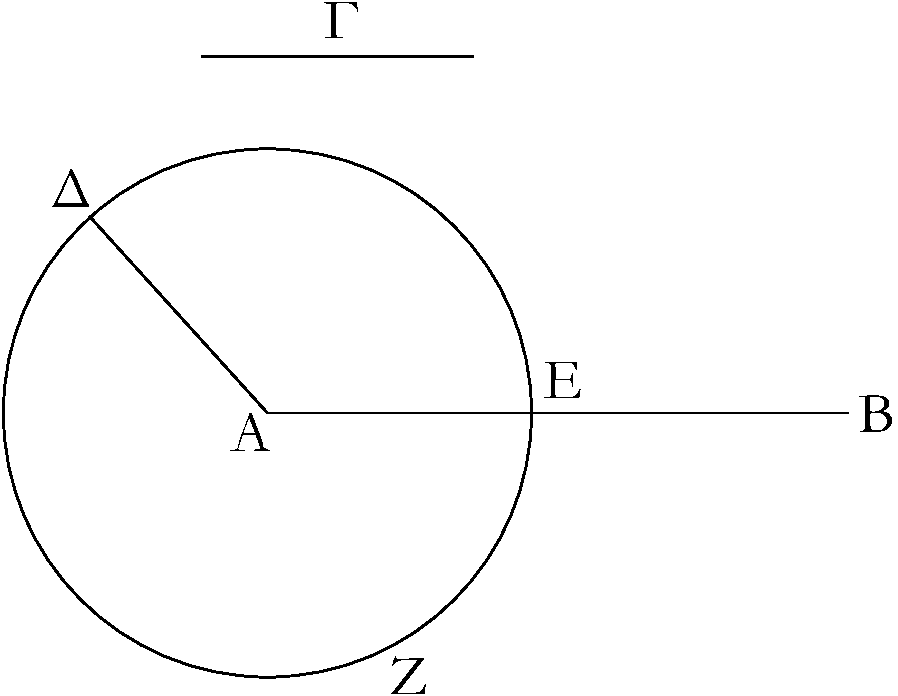
\includegraphics[width=0.8\textwidth]{Book01/fig03g.pdf}}

\gr{Δύο ἄρα δοθεισῶν εὐθειῶν ἀνίσων τῶν ΑΒ, Γ ἀπὸ τῆς μείζονος τῆς ΑΒ τῇ ἐλάσσονι τῇ Γὸίση ἀφή|ρηται ἡ ΑΕ; ὅπερ ἔδει
ποιῆσαι.}}

\ParallelRText{
\begin{center}
{\large Proposition 3}
\end{center}

For two given unequal straight-lines, to cut off from the greater a straight-line
equal to the lesser.

Let $AB$ and $C$ be the two given unequal straight-lines, of which let the greater be $AB$. So it is required to cut off a straight-line equal to the lesser $C$ from the greater $AB$.

Let the line $AD$, equal to the straight-line $C$, be placed at  point $A$ [Prop.~1.2]. And let
the circle $DEF$ be drawn with center $A$ and radius $AD$ [Post.~3].

And since  point $A$ is the center of  circle $DEF$, $AE$ is equal to $AD$ [Def.~1.15]. But,
$C$ is also equal to $AD$. Thus, $AE$ and $C$ are each equal to $AD$. So $AE$
is also equal to $C$ [C.N.~1].\\

% Removed epsf size command
\centerline{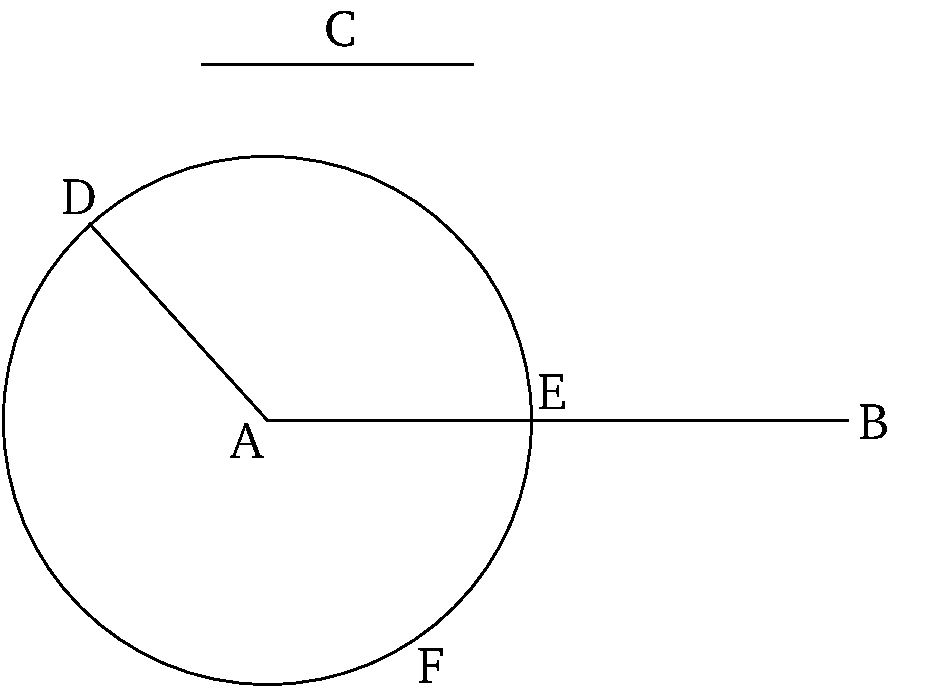
\includegraphics[width=0.8\textwidth]{Book01/fig03e.pdf}}

Thus, for two given unequal straight-lines, $AB$ and $C$, the (straight-line) $AE$, equal to
the lesser $C$, has been cut off from the greater $AB$. (Which is) the very thing it was required to do.}
\end{Parallel}

%%%%%%
% Prop 1.4
%%%%%%
\pdfbookmark[1]{Proposition 1.4}{pdf1.4}
\begin{Parallel}{}{} 
\ParallelLText{
\begin{center}
{\large \ggn{4}.}
\end{center}\vspace*{-7pt}

\gr{Ἐὰν δύο τρίγωνα τὰξ δύο πλευρὰξ [ταῖς] δυσὶ πλευραῖξ ἴσαςὸέθῃ ἑκατέραν ἑκατέρᾳ καὶ τὴν γωνίαν τῇ γωνίᾳ  ἴσηνὸέθῃ τὴν ὑπὸ τῶνὸίσων εὐθειῶν περιεθομένην, καὶ τὴν βάσιν τὴ| βάσει ἴσην ὁέχει, καὶ τὸ τρίγωνον τῷ τριγώνῳ  ἴσονὸέσται, καὶ αἱ λοιπαὶ γωνίαι ταῖς λοιπαῖξ γωνίαις ἴσαιὸέσονται ἑκατέρα ἑκατέρᾳ, ὑφὸ ὁὰξ αἱ
 ἴσαι πλευραὶ ὑποτείνουσιν.}

% Removed epsf size command
\centerline{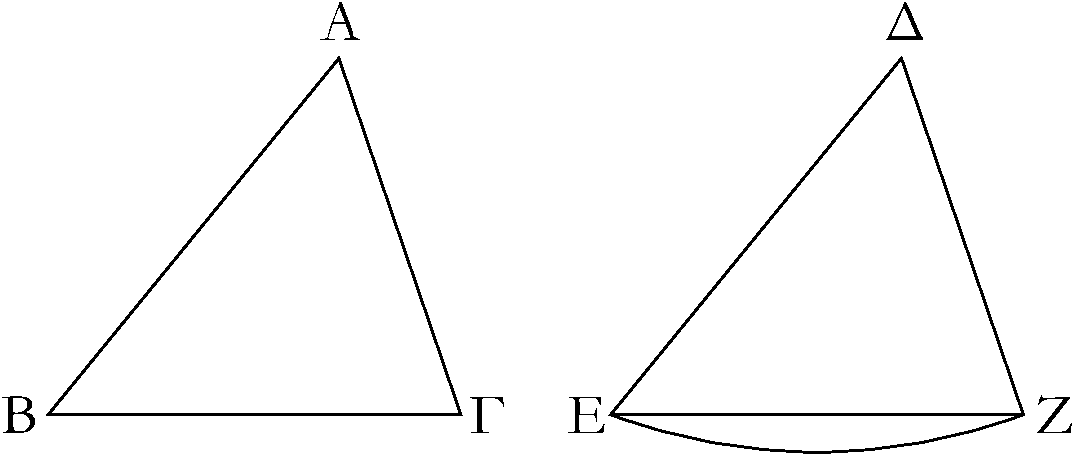
\includegraphics[width=0.8\textwidth]{Book01/fig04g.pdf}}

\gr{Ἔστω δύο τρίγωνα τὰ ΑΒΓ, ΔΕΖ τὰξ δύο πλευρὰξ τὰξ ΑΒ, ΑΓ ταῖς δυσὶ πλευραῖξ ταῖς ΔΕ, ΔΖ ἴσας ἔχοντα ἑκατέραν ἑκατέρᾳ τὴν μὲν ΑΒ τῇ ΔΕ τὴν δὲ ΑΓ τῇ ΔΖ καὶ γωνίαν τὴν ὑπὸ ΒΑΓ γωνίᾳ τῇ ὑπὸ ΕΔΖ ἴσην. λέγω, ὅτι καὶ βάσις ἡ ΒΓ βάσει τῇ ΕΖὸίση ἐστίν, καὶ τὸ ΑΒΓ τρίγωνον τῷ ΔΕΖ τριγώνῳ  ἴσονὸέσται, 
καὶ αἱ λοιπαὶ γωνίαι ταῖς λοιπαῖξ γωνίαις ἴσαιὸέσονται ἑκατέρα ἑκατέρᾳ, ὑφὸ ὁὰξ αἱ  ἴσαι πλευραὶ ὑποτείνουσιν, ἡ μὲν ὑπὸ ΑΒΓ τῇ ὑπὸ ΔΕΖ, ἡ δὲ ὑπὸ ΑΓΒ τῇ ὑπὸ ΔΖΕ.}

\gr{Ἐφαρμοζομένου γὰρ τοῦ ΑΒΓ τριγώνου ἐπὶ τὸ ΔΕΖ τρίγωνον καὶ τιθεμένου τοῦ μὲν Α σημείου ἐπὶ τὸ Δ σημεῖον τῆς δὲ ΑΒ εὐθείας ἐπὶ τὴν ΔΕ, ἐφαρμόσει καὶ τὸ Β σημεῖον ἐπὶ τὸ Ε διὰ τὸ  ἴσην εὸῖναι τὴν ΑΒ τῇ ΔΕ; ἐφαρμοσάσης δὴ τῆς ΑΒ ἐπὶ τὴν ΔΕ ἐφαρμόσει καὶ ἡ ΑΓ εὐθεῖα ἐπὶ τὴν ΔΖ διὰ τὸ  ἴσην εὸῖναι τὴν ὑπὸ ΒΑΓ γωνίαν τῇ ὑπὸ ΕΔΖ; ὁώστε καὶ τὸ Γ σημεῖον ἐπὶ τὸ Ζ σημεῖον ἐφαρμόσει διὰ τὸ  ἴσην πάλιν εὸῖναι τὴν ΑΓ τῇ ΔΖ. ἀλλὰ μὴν καὶ τὸ Β ἐπὶ τὸ Ε ἐφηρμόκει; ὁώστε βάσις ἡ ΒΓ ἐπὶ βάσιν τὴν ΕΖ ἐφαρμόσει. εἰ γὰρ τοῦ μὲν Β ἐπὶ τὸ Ε ἐφαρμόσαντος τοῦ δὲ Γ ἐπὶ τὸ Ζ ἡ ΒΓ βάσις ἐπὶ τὴν ΕΖ οὐκ ἐφαρμόσει, δύο εὐθεῖαι θωρίον περιέχουσιν; ὅπερ ἐστὶν ἀδύνατον. ἐφαρμόσει ἄρα ἡ ΒΓ βάσις ἐπὶ τὴν ΕΖ καὶ ὸίση αὐτῇ ὸέσται; ὁώστε καὶ ὅλον τὸ ΑΒΓ 
τρίγωνον ἐπὶ ὅλον τὸ ΔΕΖ τρίγωνον ἐφαρμόσει καὶ  ἴσον αὐτῷ ὸέσται, καὶ
αἱ λοιπαὶ γωνίαι ἐπὶ τὰξ λοιπὰξ γωνίας ἐφαρμόσουσι καὶ  ἴσαι αὐταῖςὸέσονται, ἡ μὲν ὑπὸ ΑΒΓ τῇ ὑπὸ ΔΕΖ ἡ δὲ ὑπὸ ΑΓΒ τῇ ὑπὸ ΔΖΕ.}

\gr{Ἐὰν ἄρα δύο τρίγωνα τὰξ δύο πλευρὰξ [ταῖς] δύο πλευραῖξ ἴσαςὸέθῃ ἑκατέραν ἑκατέρᾳ καὶ τὴν γωνίαν τῇ γωνίᾳ  ἴσηνὸέθῃ τὴν ὑπὸ τῶνὸίσων εὐθειῶν περιεθομένην, καὶ τὴν βάσιν τὴ| βάσει ἴσην ὁέχει, καὶ τὸ τρίγωνον τῷ τριγώνῳ  ἴσονὸέσται, καὶ αἱ λοιπαὶ γωνίαι ταῖς λοιπαῖξ γωνίαις ἴσαιὸέσονται ἑκατέρα ἑκατέρᾳ, ὑφὸ ὁὰξ αἱ
 ἴσαι πλευραὶ ὑποτείνουσιν; ὅπερ ἔδει δεῖχαι.}}

\ParallelRText{
\begin{center}
{\large Proposition 4}
\end{center}

If two triangles have two  sides equal to two sides, respectively, and have the
angle(s) enclosed by the equal straight-lines equal, (then)
they will also have the base equal to the base, and the triangle will be equal
to the triangle,  and
the remaining angles subtended by the equal sides will be equal to the corresponding remaining angles.

% Removed epsf size command
\centerline{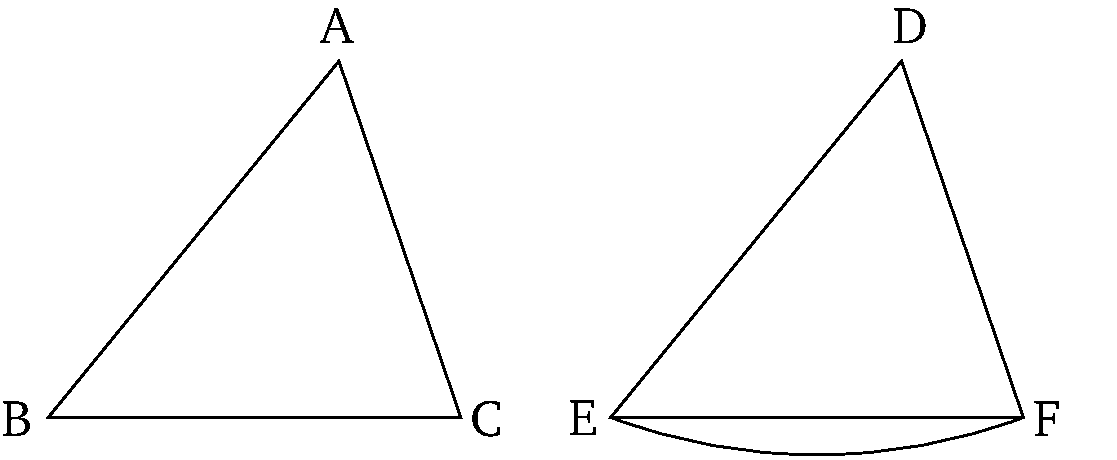
\includegraphics[width=0.8\textwidth]{Book01/fig04e.pdf}}

Let $ABC$ and $DEF$ be  two triangles having the two sides $AB$ and $AC$ equal to the two sides $DE$ and $DF$, respectively. (That is) $AB$ to $DE$, and $AC$ to $DF$. And (let) the angle $BAC$ (be) equal to the angle $EDF$. I say that the base $BC$ is also equal to the base
$EF$, and  triangle $ABC$ will be equal to triangle $DEF$, and the remaining angles
subtended by the equal sides will be equal to the corresponding remaining angles. (That is) $ABC$ to $DEF$, and $ACB$ to
$DFE$.

For if triangle $ABC$ is applied to triangle $DEF$,$^\dag$ the point $A$ being placed
on the point $D$, and the straight-line $AB$ on $DE$, (then) the point $B$ will also coincide with $E$, on account of $AB$ being equal to $DE$. So (because of) $AB$ coinciding with $DE$, the straight-line $AC$ will also coincide with $DF$, on account of the angle $BAC$ being equal to $EDF$. So the point $C$ will also coincide with the
point $F$,  again on account of $AC$ being equal to $DF$.  But,  point $B$  certainly also coincided with point $E$, so that the base $BC$ will coincide with the base $EF$.
For if $B$ coincides with $E$, and $C$ with $F$, and the base $BC$ does not coincide with $EF$, (then) two straight-lines will encompass an area. The very thing is impossible [Post.~1].$^\ddag$ Thus, the base $BC$ will coincide with $EF$, and will be equal to it [C.N.~4]. So  the whole triangle $ABC$ will coincide with the whole triangle $DEF$, and will be equal to it [C.N.~4]. And the remaining angles will coincide with the remaining angles, and  will be equal to them [C.N.~4]. (That is) $ABC$ to $DEF$, and $ACB$
to $DFE$ [C.N.~4].

Thus, if two triangles have two  sides equal to two sides, respectively, and have the
angle(s) enclosed by the equal straight-lines equal, (then)
they will also have the base equal to the base, and the triangle will be equal
to the triangle,  and
the remaining angles subtended by the equal sides will be equal to the
corresponding remaining angles. (Which is) the very thing it was required to show.}
\end{Parallel}
{\footnotesize
\noindent $^\dag$ The application of one figure to another should be counted as an additional postulate.\\[0.5ex]
$^\ddag$ Since Post.~1 implicitly assumes that the straight-line
joining two given points is unique.}

%%%%%%
% Prop 1.5
%%%%%%
\pdfbookmark[1]{Proposition 1.5}{pdf1.5}
\begin{Parallel}{}{} 
\ParallelLText{
\begin{center}
{\large \ggn{5}.}
\end{center}\vspace*{-7pt}

\gr{Τῶν ἰσοσκελῶν τριγώνων αἱ πρὸς τῇ βάσει γωνίαι ἴσαι ἀλλήλαις εἰσίν, καὶ προσεκβληθεισῶν τῶνὸίσων εὐθειῶν αἱ ὑπὸ τὴν βάσιν γωνίαι ἴσαι ἀλλήλαιςὸέσονται.}

\gr{Ἔστω τρίγωνον ἰσοσκελὲξ τὸ ΑΒΓ ἴσην ἔχον τὴν ΑΒ πλευρὰν τῇ ΑΓ πλευρᾶ|, καὶ προσεκβεβλήσθωσαν ἐπ' εὐθείας ταῖς ΑΒ,  ΑΓ εὐθεῖαι αἱ ΒΔ, ΓΕ; λέγω, ὅτι ἡ μὲν ὑπὸ ΑΒΓ γωνία τῇ ὑπὸ ΑΓΒὸίση ἐστίν, ἡ δὲ ὑπὸ ΓΒΔ τῇ ὑπὸ ΒΓΕ.}

\gr{Εἰλήφθω γὰρ ἐπὶ τῆς ΒΔ τυθὸν σημεῖον τὸ Ζ, καὶ ἀφῃρήσθω ἀπὸ τῆς μείζονος τῆς ΑΕ τῇ ἐλάσσονι τῇ ΑΖὸίση ἡ ΑΗ, καὶ ἐπεζεύθθωσαν αἱ ΖΓ, ΗΒ εὐθεῖαι.}\\

% Removed epsf size command
\centerline{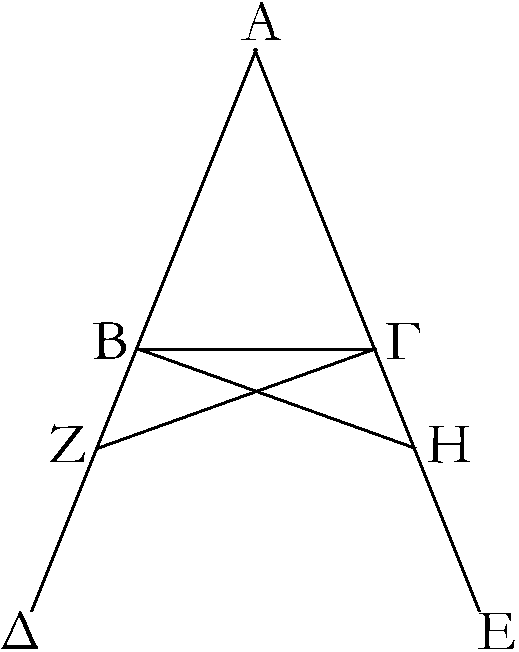
\includegraphics[width=0.8\textwidth]{Book01/fig05g.pdf}}

\gr{Ἐπεὶ οὸῦνὸίση ἐστὶν ἡ μὲν ΑΖ τῇ ΑΗ ἡ δὲ ΑΒ τῇ ΑΓ, δύο δὴ αἱ ΖΑ, ΑΓ δυσὶ ταῖς ΗΑ, ΑΒ ἴσαι εἰσὶν ἑκατέρα ἑκατέρᾳ; καὶ γωνίαν κοινὴν περιέθουσι τὴν ὑπὸ ΖΑΗ; βάσις ἄρα ἡ ΖΓ βάσει τῇ ΗΒὸίση ἐστίν, καὶ τὸ ΑΖΓ τρίγωνον τῷ ΑΗΒ τριγώνῳ  ἴσονὸέσται, καὶ αἱ λοιπαὶ γωνίαι ταῖς λοιπαῖξ γωνίαις ἴσαιὸέσονται ἑκατέρα ἑκατέρᾳ, ὑφὸ ὁὰξ αἱ  ἴσαι πλευραὶ ὑποτείνουσιν, ἡ μὲν ὑπὸ ΑΓΖ τῇ ὑπὸ ΑΒΗ, ἡ δὲ ὑπὸ ΑΖΓ τῇ ὑπὸ ΑΗΒ. καὶ ἐπεὶ ὅλη ἡ ΑΖ ὅλῃ τῇ ΑΗ ἐστινὸίση, ὁῶν ἡ ΑΒ τῇ ΑΓ ἐστινὸίση, λοιπὴ
 ἄρα ἡ ΒΖ λοιπῆ| τῇ ΓΗ ἐστινὸίση. ἐδείθθη δὲ καὶ ἡ ΖΓ τῇ ΗΒὸίση; δύο δὴ αἱ ΒΖ, ΖΓ δυσὶ ταῖς ΓΗ, ΗΒ ἴσαι εἰσὶν ἑκατέρα ἑκατέρᾳ; καὶ γωνία ἡ ὑπὸ ΒΖΓ γωνίᾳ  τῃ ὑπὸ ΓΗΒὸίση, καὶ βάσις αὐτῶν κοινὴ ἡ ΒΓ; καὶ τὸ ΒΖΓ ἄρα τρίγωνον τῷ ΓΗΒ τριγώνῳ
 ἴσονὸέσται, καὶ αἱ λοιπαὶ γωνίαι ταῖς λοιπαῖξ γωνίαις ἴσαιὸέσονται ἑκατέρα  ἑκατέρᾳ, ὑφὸ ὁὰξ αἱ  ἴσαι πλευραὶ ὑποτείνουσιν; ὸίση ἄρα ἐστὶν ἡ μὲν ὑπὸ ΖΒΓ τῇ ὑπὸ ΗΓΒ ἡ δὲ ὑπὸ ΒΓΖ τῇ ὑπὸ ΓΒΗ. ἐπεὶ οὸῦν ὅλη ἡ ὑπὸ ΑΒΗ γωνία ὅλῃ τῇ ὑπὸ ΑΓΖ γωνίᾳ ἐδείθθηὸίση, ὁῶν ἡ ὑπὸ ΓΒΗ τῇ ὑπὸ ΒΓΖὸίση, λοιπὴ
 ἄρα ἡ ὑπὸ
ΑΒΓ λοιπῆ| τῇ ὑπὸ ΑΓΒ ἐστινὸίση; καί εἰσι πρὸς τῇ βάσει τοῦ ΑΒΓ τριγώνου. ἐδείθθη δὲ καὶ ἡ ὑπὸ ΖΒΓ τῇ ὑπὸ ΗΓΒὸίση; καί εἰσιν ὑπὸ τὴν βάσιν.}

\gr{Τῶν ἄρα ἰσοσκελῶν τριγώνων αἱ τρὸξ τῇ βάσει γωνίαι ἴσαι ἀλλήλαις εἰσίν, καὶ προσεκβληθεισῶν τῶνὸίσων εὐθειῶν αἱ ὑπὸ τὴν βάσιν γωνίαι ἴσαι ἀλλήλαιςὸέσονται; ὅπερ ἔδει δεῖχαι.}}

\ParallelRText{
\begin{center}
{\large Proposition 5}
\end{center}

For isosceles triangles, the angles at the base are equal to one another, and if
the equal sides are produced (then) the angles under the base will be equal to one another.

Let $ABC$ be an isosceles triangle having the side $AB$ equal to the side $AC$, and let the straight-lines $BD$ and $CE$ be produced in a straight-line
with $AB$ and $AC$ (respectively) [Post.~2]. I say that the angle $ABC$ is equal to $ACB$, and (angle) $CBD$  to $BCE$.

For let the point $F$ be taken at random on  $BD$, and let $AG$
be cut off from the greater $AE$, equal to the lesser $AF$ [Prop.~1.3]. Also, let
the straight-lines $FC$ and $GB$ be joined [Post.~1].

% Removed epsf size command
\centerline{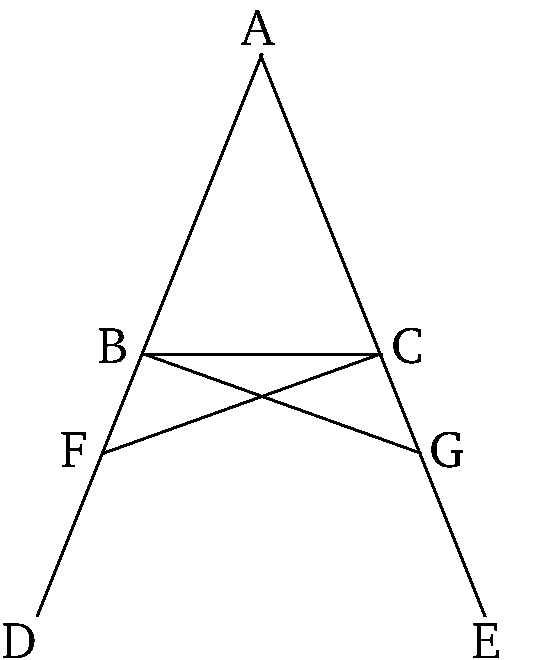
\includegraphics[width=0.8\textwidth]{Book01/fig05e.pdf}}

In fact, since $AF$ is equal to $AG$, and $AB$ to $AC$, the two (straight-lines) $FA$, $AC$ are
equal to the two (straight-lines) $GA$, $AB$, respectively. They also encompass a
common angle, $FAG$. Thus, the base $FC$ is equal to the base $GB$, and the
triangle $AFC$ will be equal to the triangle $AGB$, and the remaining angles
subtended by the equal sides will
be equal to the corresponding  remaining angles [Prop.~1.4].  (That is) $ACF$ to $ABG$, and $AFC$ to $AGB$. And since the whole of $AF$ is
equal to the whole of $AG$, within which $AB$ is equal to $AC$, the remainder
$BF$ is thus equal to the remainder $CG$ [C.N.~3]. But $FC$ was also shown (to be) equal to $GB$. So
the two (straight-lines) $BF$, $FC$ are equal to the two (straight-lines) $CG$, $GB$, respectively,
and the angle $BFC$ (is) equal to the angle $CGB$, and the base $BC$ is common to
them. Thus, the triangle $BFC$ will be equal to the triangle $CGB$, and
the remaining angles subtended by the equal sides will be equal to the corresponding remaining angles [Prop.~1.4]. Thus, $FBC$ is equal to $GCB$, and $BCF$ to
$CBG$. Therefore, since the whole angle $ABG$ was shown (to be) equal to the
whole angle $ACF$, within which $CBG$ is equal to $BCF$, the remainder $ABC$
is thus equal to the remainder $ACB$ [C.N.~3]. And they are at the base of triangle
$ABC$. And $FBC$ was also shown (to be) equal to $GCB$. And they are under
the base.

Thus, for isosceles triangles, the angles at the base are equal to one another, and if
the equal sides are produced (then) the angles under the base will be equal to one another. (Which is) the very thing it was required to show.}
\end{Parallel}

%%%%%%
% Prop 1.6
%%%%%%
\pdfbookmark[1]{Proposition 1.6}{pdf1.6}
\begin{Parallel}{}{} 
\ParallelLText{
\begin{center}
{\large \ggn{6}.}
\end{center}\vspace*{-7pt}

\gr{Ἐὰν τριγώνου αἱ δύο γωνίαι ἴσαι ἀλλήλαις ὦσιν, καὶ αἱ ὑπὸ
τὰξ ἴσας γωνίας ὑποτείνουσαι πλευραὶ  ἴσαι ἀλλήλαιςὸέσονται.}

\gr{Ἔστω τρίγωνον τὸ ΑΒΓ ἴσην ἔχον τὴν ὑπὸ ΑΒΓ γωνίαν τῇ ὑπὸ ΑΓΒ γωνίᾳ; λέγω, ὅτι καὶ πλευρὰ ἡ ΑΒ πλευρᾶ| τῇ ΑΓ ἐστινὸίση.}

% Removed epsf size command
\centerline{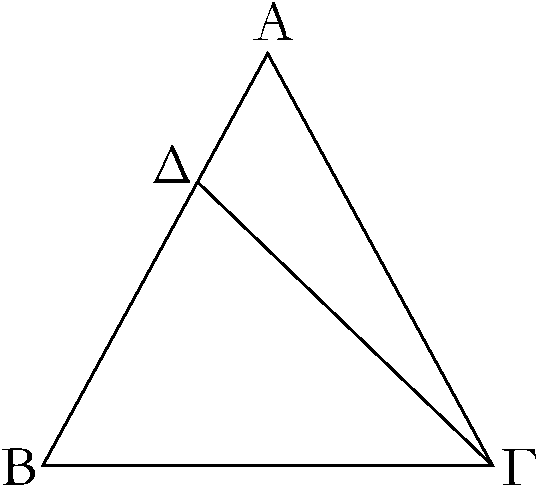
\includegraphics[width=0.8\textwidth]{Book01/fig06g.pdf}}

\gr{Εἰ γὰρὸάνισόξ ἐστιν ἡ ΑΒ τῇ ΑΓ, ἡ ἑτέρα αὐτῶν μείζων ἐστίν. ὸέστω μείζων ἡ ΑΒ, καὶ ἀφῃρήσθω ἀπὸ τῆς μείζονος τῆς ΑΒ τῇ
ἐλάττονι τῇ ΑΓὸίση ἡ ΔΒ, καὶ ἐπεζεύθθω ἡ ΔΓ.}

\gr{Ἐπεὶ οὸῦνὸίση ἐστὶν ἡ ΔΒ τῇ ΑΓ κοινὴ δὲ ἡ ΒΓ, δύο
δὴ αἱ ΔΒ, ΒΓ δύο ταῖς ΑΓ, ΓΒ ἴσαι εἰσὶν ἑκατέρα ἑκατέρᾳ, καὶ
γωνία ἡ ὑπὸ ΔΒΓ γωνίᾳ τῇ ὑπὸ ΑΓΒ ἐστινὸίση; βάσις ἄρα
ἡ ΔΓ βάσει τῇ ΑΒὸίση ἐστίν, καὶ τὸ ΔΒΓ τρίγωνον τῷ ΑΓΒ
τριγώνῳ  ἴσονὸέσται, τὸ ὸέλασσον τῷ μείζονι; ὅπερὸάτοπον;
οὐκ ἄραὸάνισόξ ἐστιν ἡ ΑΒ τῇ ΑΓ; ὸίση ἄρα.}

\gr{Ἐὰν ἄρα  τριγώνου αἱ δὑο γωνίαι ἴσαι ἀλλήλαις ὦσιν, καὶ αἱ ὑπὸ
τὰξ ἴσας γωνίας ὑποτείνουσαι πλευραὶ  ἴσαι ἀλλήλαιςὸέσονται;
ὅπερ ἔδει δεῖχαι.}}

\ParallelRText{
\begin{center}
{\large Proposition 6}
\end{center}

If a triangle has two angles equal to one another (then) the sides subtending the
equal angles will also be equal to one another.

Let $ABC$ be a triangle having the angle $ABC$ equal to the angle $ACB$. I say that
side $AB$ is also equal to side $AC$.\\

% Removed epsf size command
\centerline{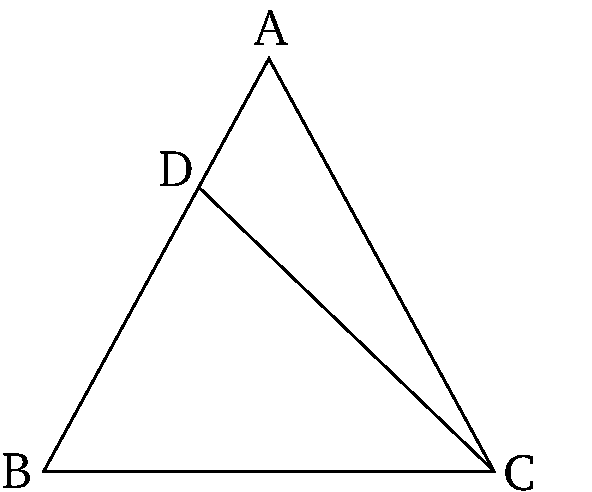
\includegraphics[width=0.8\textwidth]{Book01/fig06e.pdf}}

For if $AB$ is unequal to $AC$ (then) one of them is greater. Let $AB$ be greater. And
let $DB$, equal to the lesser $AC$, be cut off from the greater $AB$ [Prop.~1.3].  And
let $DC$ be joined [Post.~1].

Therefore, since $DB$ is equal to $AC$, and $BC$ (is) common, the two sides $DB$, $BC$ are equal to the two sides $AC$, $CB$, respectively, and the angle $DBC$
is equal to the angle $ACB$. Thus, the base $DC$ is equal to the base
$AB$, and the triangle $DBC$ will be equal to the triangle $ACB$ [Prop.~1.4], the lesser
to the greater. The very notion (is) absurd [C.N.~5]. Thus, $AB$ is not unequal
to $AC$. Thus, (it is) equal.$^\dag$

Thus, if a triangle has two angles equal to one another (then) the sides subtending the
equal angles will also be equal to one another. (Which is) the very thing it was required to show.}
\end{Parallel}
{\footnotesize \noindent $^\dag$ Here, use is made of the previously
unmentioned common notion that if two quantities are not unequal then they must be equal. Later on, use is made of the closely related common notion
that if two quantities are not greater than or less than one another, respectively, then they must be equal to one another.}

%%%%%%
% Prop 1.7
%%%%%%
\pdfbookmark[1]{Proposition 1.7}{pdf1.7}
\begin{Parallel}{}{} 
\ParallelLText{
\begin{center}
{\large \ggn{7}.}
\end{center}\vspace*{-7pt}

\gr{Ἐπὶ τῆς αὐτῆς εὐθείας δύο ταῖς αὐταῖς εὐθείαιςὸάλλαι δύο
εὐθεῖαι ἴσαι ἑκατέρα ἑκατέρᾳ οὐ συσταθήσονται πρὸςὸάλλῳ καὶ ὸάλλῳ
σημείῳ ἐπὶ τὰ αὐτὰ μέρη τὰ αὐτὰ πέραταὸέθουσαι ταῖς ἐξ ἀρθῆς
εὐθείαις.}\\

% Removed epsf size command
\centerline{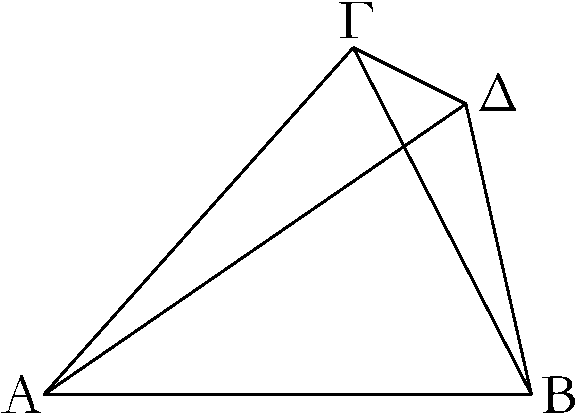
\includegraphics[width=0.8\textwidth]{Book01/fig07g.pdf}}

\gr{Εἰ γὰρ δυνατόν, ἐπὶ τῆς αὐτῆς εὐθείας τῆς ΑΒ δύο ταῖς αὐταῖς
εὐθείαις ταῖς ΑΓ, ΓΒὸάλλαι δύο εὐθεῖαι αἱ ΑΔ, ΔΒ ἴσαι
ἑκατέρα ἑκατέρᾳ συνεστάτωσαν πρὸςὸάλλῳ καὶ ὸάλλῳ σημείῳ τῷ
τε Γ καὶ Δ ἐπὶ τὰ αὐτὰ μέρη τὰ αὐτὰ πέραταὸέθουσαι, ὁώστε ἴσην εὸῖναι τὴν
μὲν ΓΑ τῇ ΔΑ τὸ αὐτὸ πέραςὸέθουσαν αὐτῇ τὸ Α, τὴν δὲ
ΓΒ τῇ ΔΒ τὸ αὐτὸ πέραςὸέθουσαν αὐτῇ τὸ Β, καὶ 
ἐπεζεύθθω ἡ ΓΔ.}

\gr{Ἐπεὶ οὸῦνὸίση ἐστὶν ἡ ΑΓ τῇ  ΑΔ, ὸίση ἐστὶ καὶ  γωνία ἡ ὑπὸ
ΑΓΔ τῇ ὑπὸ ΑΔΓ; μείζων ἄρα ἡ ὑπὸ ΑΔΓ τῆς ὑπὸ ΔΓΒ; πολλῶ|
 ἄρα ἡ ὑπὸ ΓΔΒ μείζων ἐστί τῆς ὑπὸ ΔΓΒ. πάλιν ἐπεὶ
ὸίση ἐστὶν ἡ ΓΒ τῇ ΔΒ, ὸίση ἐστὶ καὶ γωνία ἡ ὑπὸ ΓΔΒ
γωνίᾳ τῇ ὑπὸ ΔΓΒ. ἐδείθθη δὲ αὐτῆς καὶ πολλῶ| μείζων;
ὅπερ ἐστὶν ἀδύνατον.}

\gr{Οὐκ ἄρα ἐπὶ τῆς αὐτῆς εὐθείας δύο ταῖς αὐταῖς εὐθείαιςὸάλλαι δύο
εὐθεῖαι ἴσαι ἑκατέρα ἑκατέρᾳ  
συσταθήσονται πρὸςὸάλλῳ καὶ ὸάλλῳ
σημείῳ ἐπὶ τὰ αὐτὰ μέρη τὰ αὐτὰ πέραταὸέθουσαι ταῖς ἐξ ἀρθῆς
εὐθείαις;  ὅπερ ἔδει δεῖχαι.}}

\ParallelRText{
\begin{center}
{\large Proposition 7}
\end{center}

On the same straight-line, two other straight-lines 
equal, respectively, to 
two (given) straight-lines (which meet) cannot be constructed (meeting)
at  a different point on the same
side (of the straight-line), but having the same ends as the given straight-lines.

% Removed epsf size command
\centerline{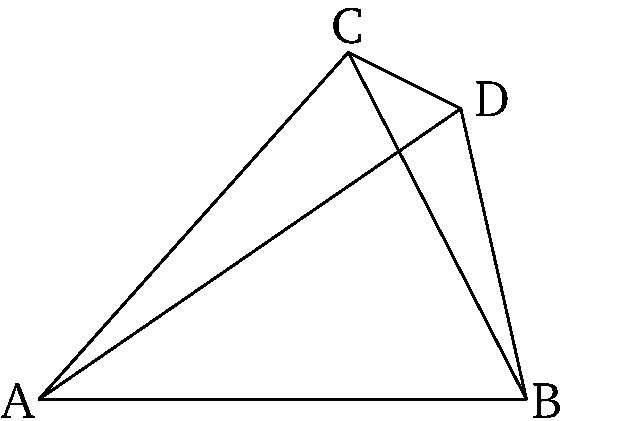
\includegraphics[width=0.8\textwidth]{Book01/fig07e.pdf}}

For, if possible, let the two straight-lines $AC$, $CB$, equal to two other straight-lines $AD$, $DB$, respectively, be constructed
on the same straight-line $AB$, meeting at different points, $C$ and $D$, on the
same side (of $AB$), and having the same ends (on $AB$). So $CA$ is equal to $DA$, having the same end $A$ as it, and $CB$ is equal to $DB$, having the
same end $B$ as it. And let $CD$ be joined [Post.~1].

Therefore, since $AC$ is equal to $AD$,  the angle $ACD$ is also equal to angle $ADC$ [Prop.~1.5].
Thus, $ADC$ (is) greater than $DCB$ [C.N.~5]. Thus, $CDB$ is much greater
than $DCB$ [C.N.~5]. Again, since  $CB$ is equal to $DB$, the angle $CDB$ is also equal to
angle $DCB$ [Prop.~1.5]. But it was shown that the former (angle) is also much
greater (than the latter). The very thing is impossible.

Thus, on the same straight-line, two other straight-lines equal, respectively, to  
two (given) straight-lines  (which meet) cannot be constructed (meeting)
at a different point on the same
side (of the straight-line), but having the same ends as the given straight-lines.
(Which is) the very thing it was required to show.}
\end{Parallel}

%%%%%%
% Prop 1.8
%%%%%%
\pdfbookmark[1]{Proposition 1.8}{pdf1.8}
\begin{Parallel}{}{} 
\ParallelLText{
\begin{center}
{\large \ggn{8}.}
\end{center}\vspace*{-7pt}

\gr{Ἐὰν δύο τρίγωνα τὰξ δύο πλευρὰξ [ταῖς] δύο πλευραῖξ ἴσαςὸέθῃ
ἑκατέραν ἑκατέρᾳ, ὸέθῃ δὲ καὶ τὴν βάσιν τῇ βάσει ἴσην, καὶ
τὴν γωνίαν τῇ γωνίᾳ  ἴσην ὁέχει τὴν ὑπὸ τῶνὸίσων
εὐθειῶν περιεθομένην.}

\gr{Ἔστω δύο τρίγωνα τὰ ΑΒΓ, ΔΕΖ τὰξ δύο πλευρὰξ τὰξ ΑΒ, ΑΓ ταῖς δύο πλευραῖξ ταῖς ΔΕ, ΔΖ ἴσας ἔχοντα ἑκατέραν ἑκατέρᾳ, τὴν μὲν ΑΒ τῇ ΔΕ τὴν δὲ ΑΓ τῇ ΔΖ; ἐθέτω δὲ καὶ βάσιν τὴν ΒΓ βάσει τῇ ΕΖ ἴσην; λέγω, ὅτι καὶ γωνία ἡ ὑπὸ ΒΑΓ γωνίᾳ τῇ ὑπὸ ΕΔΖ ἐστινὸίση.}

% Removed epsf size command
\centerline{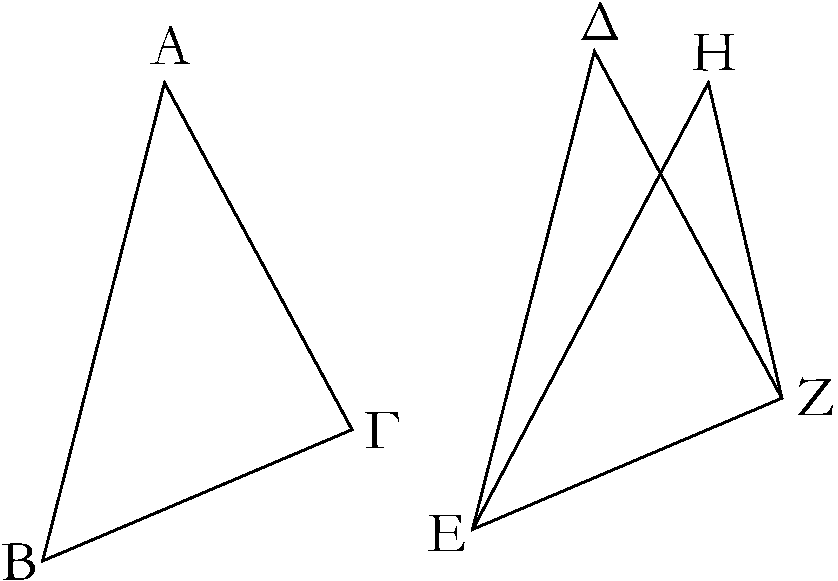
\includegraphics[width=0.8\textwidth]{Book01/fig08g.pdf}}

\gr{Ἐφαρμοζομένου γὰρ τοῦ ΑΒΓ τριγώνου ἐπὶ τὸ ΔΕΖ τρίγωνον
καὶ τιθεμένου τοῦ μὲν Β σημείου ἐπὶ τὸ Ε σημεῖον τῆς δὲ ΒΓ εὐθείας ἐπὶ τὴν ΕΖ ἐφαρμόσει καὶ τὸ Γ σημεῖον ἐπὶ τὸ Ζ
διὰ τὸ  ἴσην εὸῖναι τὴν ΒΓ τῇ ΕΖ; ἐφαρμοσάσης δὴ τῆς ΒΓ ἐπὶ τὴν ΕΖ ἐφαρμόσουσι καὶ αἱ ΒΑ, ΓΑ ἐπὶ τὰξ ΕΔ, ΔΖ. εἰ γὰρ
βάσις μὲν ἡ ΒΓ ἐπὶ βάσιν τὴν ΕΖ ἐφαρμόσει, αἱ δὲ ΒΑ, ΑΓ
πλευραὶ ἐπὶ τὰξ ΕΔ, ΔΖ οὐκ ἐφαρμόσουσιν ἀλλὰ παραλλάχουσιν ὡξ
αἱ ΕΗ, ΗΖ, συσταθήσονται ἐπὶ τῆς αὐτῆς εὐθείας δύο ταῖς αὐταῖς εὐθείαιςὸάλλαι δύο εὐθεῖαι ἴσαι ἑκατέρα ἑκατέρᾳ πρὸςὸάλλῳ καὶ
ὸάλλῳ σημείῳ ἐπὶ τὰ αὐτὰ μέρη τὰ αὐτὰ πέραταὸέθουσαι. οὐ
συνίστανται δέ; οὐκ ἄρα ἐφαρμοζομένης τῆς ΒΓ βάσεως ἐπὶ τὴν
ΕΖ βάσιν οὐκ
ἐφαρμόσουσι καὶ αἱ ΒΑ, ΑΓ πλευραὶ
ἐπὶ τὰξ ΕΔ, ΔΖ. ἐφαρμόσουσιν ἄρα;
ὁώστε καὶ γωνία ἡ ὑπὸ ΒΑΓ ἐπὶ  γωνίαν τὴν ὑπὸ
ΕΔΖ ἐφαρμόσει καὶ ὸίση αὐτῇ ὸέσται.}

\gr{Ἐὰν ἄρα δύο τρίγωνα τὰξ δύο πλευρὰξ [ταῖς] δύο πλευραῖξ ἴσαςὸέθῃ
ἑκατέραν ἑκατέρᾳ  καὶ τὴν βάσιν τῇ βάσει ἴσηνὸέθῃ, καὶ
τὴν γωνίαν τῇ γωνίᾳ  ἴσην ὁέχει τὴν ὑπὸ τῶνὸίσων
εὐθειῶν περιεθομένην; ὅπερ ἔδει δεῖχαι.}}

\ParallelRText{
\begin{center}
{\large Proposition 8}
\end{center}

If two triangles have  two sides equal to two sides, respectively, 
and also have the base equal to the base, (then) they will
also have equal the angles  encompassed by
the equal straight-lines.

Let $ABC$ and $DEF$ be two triangles having the two sides $AB$ and $AC$ equal to the two
sides $DE$ and $DF$, respectively. (That is) $AB$ to $DE$, and $AC$ to $DF$.  Let them also have
the base $BC$ equal to the base $EF$. I say that the angle $BAC$ is also equal
to the angle $EDF$.

% Removed epsf size command
\centerline{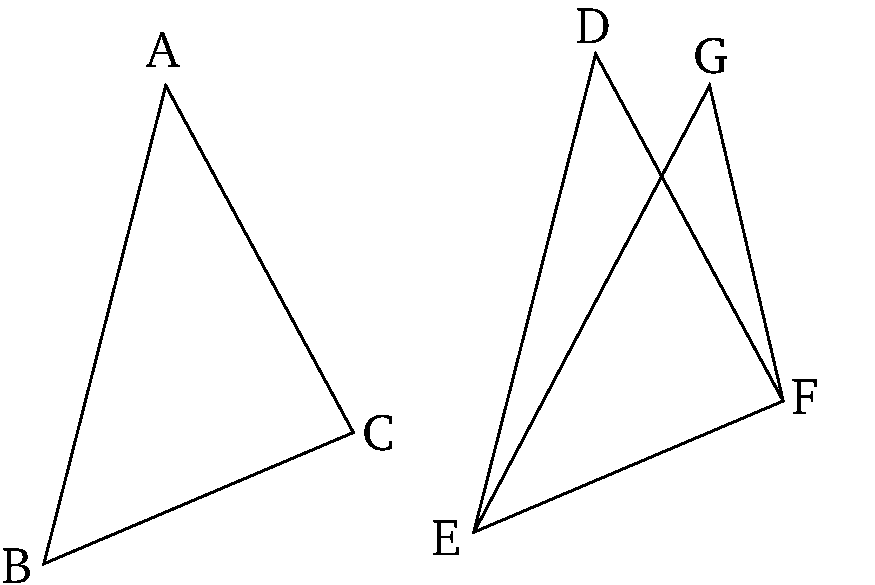
\includegraphics[width=0.8\textwidth]{Book01/fig08e.pdf}}

For if triangle $ABC$ is applied to triangle $DEF$, the point $B$ being placed on
point $E$, and the straight-line $BC$ on $EF$, (then) point $C$ will also coincide with $F$, on
account of $BC$ being equal to $EF$.
So  (because of) $BC$ coinciding with $EF$,  (the sides) $BA$ and $CA$ will also
coincide with  $ED$ and $DF$ (respectively). 
For if base $BC$ coincides with base $EF$, but the sides $AB$ and $AC$ 
do not coincide with $ED$ and $DF$ (respectively), but miss like $EG$
and $GF$ (in the above figure), 
then we will have constructed upon the same straight-line two other straight-lines equal, respectively, to two (given) straight-lines,  and (meeting)
at a different point on the same
side (of the straight-line), but having the same ends. But (such straight-lines) cannot be constructed [Prop.~1.7].
Thus,  the base $BC$ being applied to the  base $EF$,  the sides $BA$ and $AC$
cannot not coincide with $ED$ and $DF$ (respectively). Thus, they
will coincide. So the angle $BAC$ will also coincide with angle $EDF$,
and will be equal to it [C.N.~4].

Thus, if two triangles have  two  sides equal to two side, respectively,
and  have the base equal to the base, (then) they will also have equal the angles  encompassed by
the equal straight-lines. (Which is) the very thing it was required to show.}
\end{Parallel}

%%%%%%
% Prop 1.9
%%%%%%
\pdfbookmark[1]{Proposition 1.9}{pdf1.9}
\begin{Parallel}{}{} 
\ParallelLText{
\begin{center}
{\large \ggn{9}.}
\end{center}\vspace*{-7pt}

\gr{Τὴν δοθεῖσαν γωνίαν εὐθύγραμμον δίθα τεμεῖν.}

\gr{Ἔστω ἡ δοθεῖσα γωνία εὐθύγραμμος ἡ ὑπὸ ΒΑΓ. δεῖ δὴ
αὐτὴν δίθα τεμεῖν.}

\gr{Εἰλήφθω ἐπὶ τῆς ΑΒ τυθὸν σημεῖον τὸ Δ, καὶ ἀφῃρήσθω ἀπὸ
τῆς ΑΓ τῇ ΑΔὸίση ἡ ΑΕ, καὶ ἐπεζεύθθω ἡ ΔΕ, καὶ συνεστάτω
ἐπὶ τῆς ΔΕ τρίγωνον ἰσόπλευρον τὸ ΔΕΖ, καὶ ἐπεζεύθθω ἡ ΑΖ; λέγω, ὅτι ἡ ὑπὸ ΒΑΓ γωνία δίθα τέτμ  ηται ὑπὸ τῆς ΑΖ
εὐθείας.}

\gr{Ἐπεὶ γὰρὸίση ἐστὶν ἡ ΑΔ τῇ ΑΕ, κοινὴ δὲ ἡ ΑΖ, δύο δὴ αἱ ΔΑ, ΑΖ δυσὶ ταῖς ΕΑ, ΑΖ ἴσαι εἰσὶν ἑκατέρα ἑκατέρᾳ. καὶ βάσις ἡ ΔΖ
βάσει τῇ ΕΖὸίση ἐστίν; γωνία ἄρα ἡ ὑπὸ ΔΑΖ γωνίᾳ τῇ
ὑπὸ ΕΑΖὸίση ἐστίν.}

% Removed epsf size command
\centerline{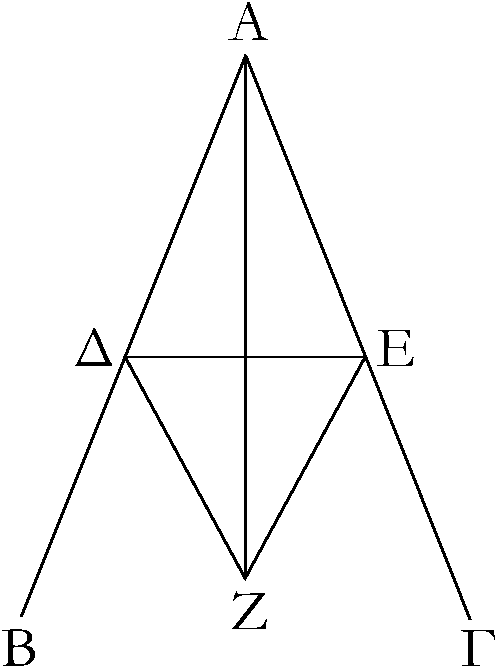
\includegraphics[width=0.8\textwidth]{Book01/fig09g.pdf}}

\gr{Ἡ  ἄρα δοθεῖσα γωνία εὐθύγραμμος ἡ ὑπὸ ΒΑΓ δίθα τέτμ  ηται
ὑπὸ τῆς ΑΖ εὐθείας; ὅπερ ἔδει ποιῆσαι.}}

\ParallelRText{
\begin{center}
{\large Proposition 9}
\end{center}

To cut a given rectilinear angle in half.

Let $BAC$ be the given rectilinear angle. So it is required to
cut it in half.

Let the point $D$ be taken at random on $AB$,
and let $AE$, equal to $AD$,  be cut off from $AC$  [Prop.~1.3], and
let $DE$ be joined. And let the equilateral triangle $DEF$
be constructed upon $DE$ [Prop.~1.1], and let $AF$ be
joined. I say that the angle $BAC$ has been cut in half by the straight-line
$AF$.

For since $AD$ is equal to  $AE$, and $AF$ is common, the two (straight-lines) $DA$,
$AF$ are equal to the two (straight-lines) $EA$, $AF$, respectively. And the base $DF$
is equal to the base $EF$. Thus, angle $DAF$ is equal to angle $EAF$ [Prop.~1.8].

% Removed epsf size command
\centerline{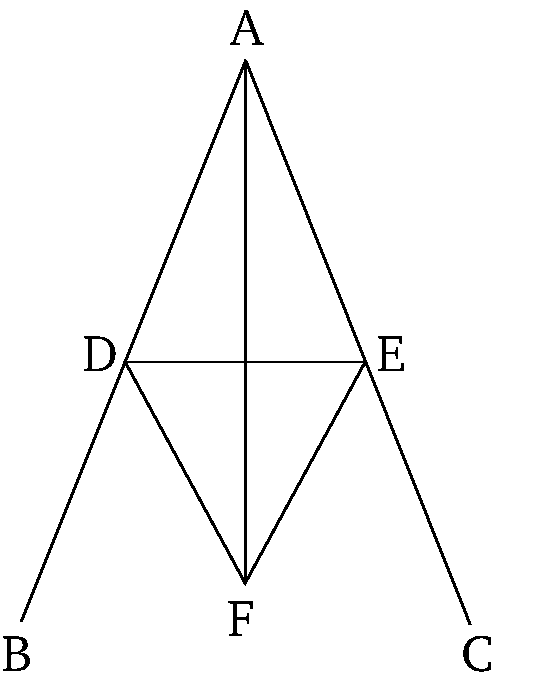
\includegraphics[width=0.8\textwidth]{Book01/fig09e.pdf}}

Thus, the given rectilinear angle $BAC$ has been cut in half by the
straight-line $AF$. (Which is) the very thing it was required to do.}
\end{Parallel}

%%%%%%
% Prop 1.10
%%%%%%
\pdfbookmark[1]{Proposition 1.10}{pdf1.10}
\begin{Parallel}{}{} 
\ParallelLText{
\begin{center}
{\large \ggn{10}.}
\end{center}\vspace*{-7pt}

\gr{Τὴν δοθεῖσαν εὐθεῖαν πεπερασμένην δίθα τεμεῖν.}

\gr{Ἔστω ἡ δοθεῖσα εὐθεῖα πεπερασμένη ἡ ΑΒ; δεῖ δὴ τὴν ΑΒ εὐθεῖαν πεπερασμένην δίθα τεμεῖν.}

\gr{Συνεστάτω ἐπ' αὐτῆς τρίγωνον ἰσόπλευρον τὸ ΑΒΓ, καὶ τετμήσθω ἡ ὑπὸ ΑΓΒ γωνία δίθα τῇ ΓΔ εὐθείᾳ; λέγω, ὅτι ἡ ΑΒ εὐθεῖα
δίθα τέτμ  ηται κατὰ τὸ Δ σημεῖον.}\\

% Removed epsf size command
\centerline{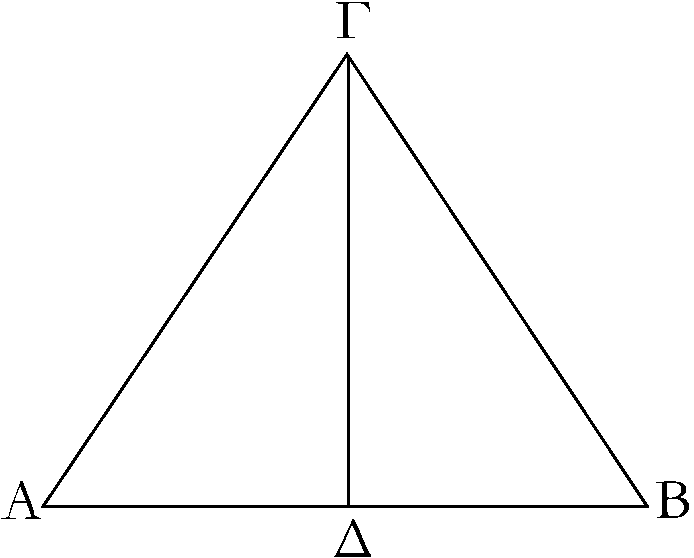
\includegraphics[width=0.8\textwidth]{Book01/fig10g.pdf}}

\gr{Ἐπεὶ γὰρὸίση ἐστὶν ἡ ΑΓ τῇ ΓΒ, κοινὴ δὲ ἡ ΓΔ, δύο δὴ αἱ
ΑΓ, ΓΔ δύο ταῖς ΒΓ, ΓΔ ἴσαι εἰσὶν ἑκατέρα ἑκατέρᾳ; καὶ γωνία
ἡ ὑπὸ ΑΓΔ γωνίᾳ τῇ ὑπὸ ΒΓΔὸίση ἐστίν; βάσις ἄρα ἡ
ΑΔ βάσει τῇ ΒΔὸίση ἐστίν.}

\gr{Ἡ  ἄρα δοθεῖσα εὐθεῖα πεπερασμένη ἡ ΑΒ δίθα τέτμ  ηται κατὰ τὸ
Δ; ὅπερ ἔδει ποιῆσαι.}}

\ParallelRText{
\begin{center}
{\large Proposition 10}
\end{center}

To cut a given finite straight-line in half.

Let $AB$ be the given finite straight-line. So it is required to cut the
finite straight-line $AB$ in half.

Let the equilateral triangle $ABC$ be constructed upon  ($AB$)
[Prop.~1.1], and let the angle $ACB$ be cut in half by the
straight-line $CD$ [Prop.~1.9]. I say that the straight-line $AB$ has been
cut in half at  point $D$.

% Removed epsf size command
\centerline{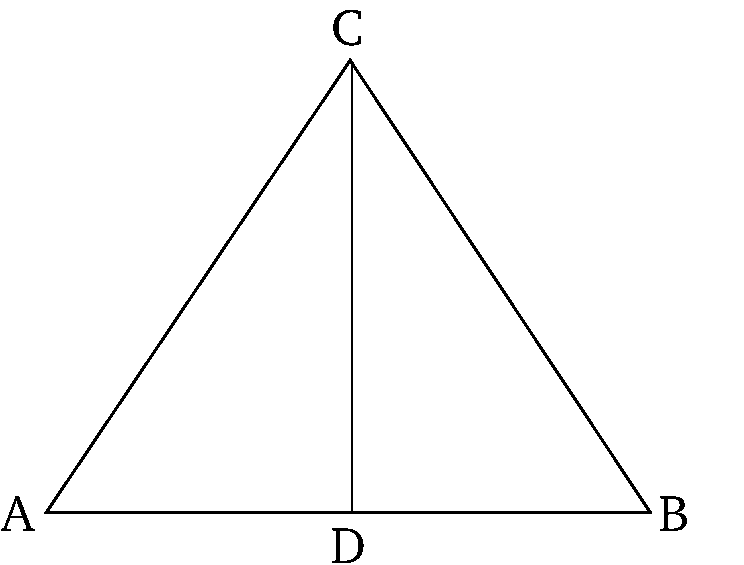
\includegraphics[width=0.8\textwidth]{Book01/fig10e.pdf}}

For since $AC$ is equal to $CB$, and $CD$ (is) common, the two (straight-lines) $AC$, $CD$
are equal to the two (straight-lines) $BC$, $CD$, respectively. And the angle $ACD$ is
equal to the angle $BCD$. Thus, the base $AD$ is equal to the base $BD$
[Prop.~1.4].

Thus, the given finite straight-line $AB$ has been cut in half at  (point) $D$. 
(Which is) the
very thing it was required to do.}
\end{Parallel}

%%%%%%
% Prop 1.11
%%%%%%
\pdfbookmark[1]{Proposition 1.11}{pdf1.11}
\begin{Parallel}{}{} 
\ParallelLText{
\begin{center}
{\large \ggn{11}.}
\end{center}\vspace*{-7pt}

\gr{Τῆ| δοθείσῃ εὐθείᾳ ἀπὸ τοῦ πρὸς αὐτῇ δοθέντος σημείου
πρὸς ὀρθὰξ γωνίας εὐθεῖαν γραμμὴν ἀγαγεῖν.}

\gr{Ἔστω ἡ μὲν δοθεῖσα εὐθεῖα ἡ ΑΒ τὸ δὲ δοθὲν σημεῖον
ἐπ' αὐτῆς τὸ Γ; δεῖ δὴ ἀπὸ τοῦ Γ σημείου τῇ ΑΒ εὐθείᾳ
πρὸς ὀρθὰξ γωνίας εὐθεῖαν γραμμὴν ἀγαγεῖν.}

% Removed epsf size command
\centerline{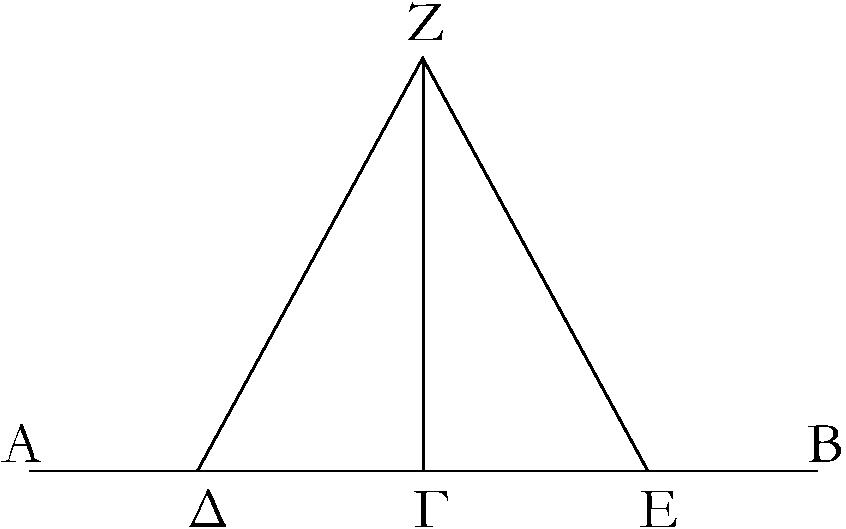
\includegraphics[width=0.8\textwidth]{Book01/fig11g.pdf}}

\gr{Εἰλήφθω ἐπὶ τῆς ΑΓ τυθὸν σημεῖον τὸ Δ, καὶ κείσθω τῇ
ΓΔὸίση ἡ ΓΕ, καὶ συνεστάτω ἐπὶ τῆς ΔΕ τρίγωνον ἰσόπλευρον
τὸ ΖΔΕ, καὶ ἐπεζεύθθω ἡ ΖΓ; λέγω, ὅτι τῇ δοθείσῃ
εὐθείᾳ τῇ ΑΒ ἀπὸ τοῦ πρὸς αὐτῇ δοθέντος σημείου τοῦ
Γ πρὸς ὀρθὰξ γωνίας εὐθεῖα γραμμὴ ὸῆκται ἡ ΖΓ.}

\gr{Ἐπεὶ γὰρὸίση ἐστὶν ἡ ΔΓ τῇ ΓΕ, κοινὴ δὲ ἡ ΓΖ, δύο δὴ
αἱ ΔΓ, ΓΖ δυσὶ ταῖς ΕΓ, ΓΖ ἴσαι εἰσὶν ἑκατέρα ἑκατέρᾳ;
καὶ βάσις ἡ ΔΖ βάσει τῇ ΖΕὸίση ἐστίν; γωνία ἄρα ἡ ὑπὸ
ΔΓΖ γωνίᾳ τῇ ὑπὸ ΕΓΖὸίση ἐστίν; καί εἰσιν ἐφεχῆς.
ὅταν δὲ εὐθεῖα ἐπ' εὐθεῖαν σταθεῖσα τὰξ ἐφεχῆς γωνίας ἴσας ἀλλήλαις ποιῆ|, ὀρθὴ ἑκατέρα τῶνὸίσων γωνιῶν
ἐστιν; ὀρθὴ  ἄρα ἐστὶν ἑκατέρα τῶν ὑπὸ ΔΓΖ, ΖΓΕ.}

\gr{Τῆ|  ἄρα δοθείσῃ εὐθείᾳ τῇ ΑΒ ἀπὸ τοῦ πρὸς αὐτῇ
δοθέντος σημείου τοῦ Γ πρὸς ὀρθὰξ γωνίας εὐθεῖα γραμμὴ
ὸῆκται ἡ ΓΖ; ὅπερ ἔδει ποιῆσαι.}}

\ParallelRText{
\begin{center}
{\large Proposition 11}
\end{center}

To draw a straight-line at right-angles to a given straight-line from a given point on it.

Let $AB$ be the given straight-line, and $C$ the given point on it. So it is required
to draw a straight-line from the point $C$ at right-angles to the straight-line $AB$.

% Removed epsf size command
\centerline{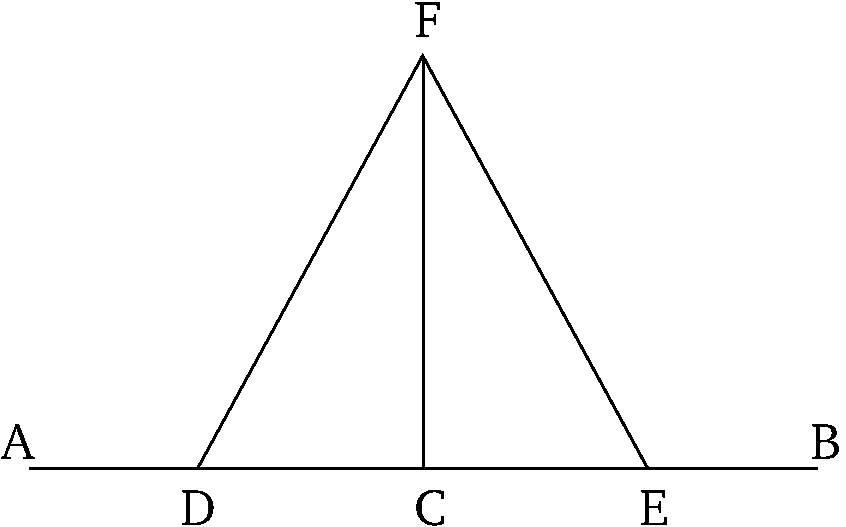
\includegraphics[width=0.8\textwidth]{Book01/fig11e.pdf}}

Let the point $D$ be be taken at random on $AC$, and let $CE$ be made equal to $CD$ [Prop.~1.3], and let the equilateral triangle $FDE$
be constructed on $DE$ [Prop.~1.1], and let $FC$ be
joined. I say that the straight-line $FC$ has been drawn at right-angles
to the given straight-line $AB$ from the given point $C$ on it.

For since $DC$ is equal to $CE$, and $CF$ is common, the two (straight-lines) $DC$, $CF$
are equal to the two (straight-lines), $EC$, $CF$, respectively.  And the base $DF$
is equal to the base $FE$. Thus, the angle $DCF$ is equal to the
angle $ECF$ [Prop.~1.8], and they are adjacent. But when a straight-line stood on 
a(nother) straight-line makes the adjacent angles equal to one another, each of the
equal angles is a right-angle [Def.~1.10]. Thus, each of the (angles)
$DCF$ and $FCE$ is a right-angle.

Thus, the straight-line $CF$ has been drawn at right-angles to the
given straight-line $AB$ from the given point $C$ on it. (Which is) the very thing
it was required to do.}
\end{Parallel}

%%%%%%
% Prop 1.12
%%%%%%
\pdfbookmark[1]{Proposition 1.12}{pdf1.12}
\begin{Parallel}{}{} 
\ParallelLText{
\begin{center}
{\large \ggn{12}.}
\end{center}\vspace*{-7pt}

\gr{Ἐπὶ τὴν δοθεῖσαν εὐθεῖαν ἄπειρον ἀπὸ τοῦ δοθέντος σημείου, ὃ μή
ἐστιν ἐπ' αὐτῆς, κάθετον εὐθεῖαν γραμμὴν ἀγαγεῖν.}

% Removed epsf size command
\centerline{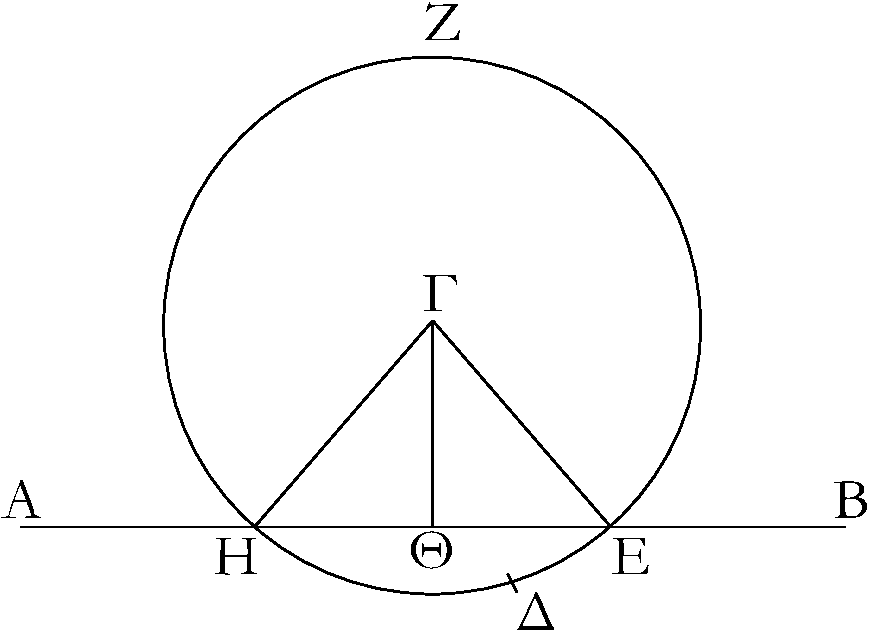
\includegraphics[width=0.8\textwidth]{Book01/fig12g.pdf}}

\gr{Ἔστω ἡ μὲν δοθεῖσα εὐθεῖαὸάπειρος ἡ ΑΒ τὸ δὲ δοθὲν σημεῖον,
ὃ μή ἐστιν ἐπ' αὐτῆς, τὸ Γ; δεῖ δὴ ἐπὶ τὴν δοθεῖσαν εὐθεῖαν ἄπειρον τὴν ΑΒ ἀπὸ τοῦ δοθέντος σημείου τοῦ Γ, ὃ μή ἐστιν
ἐπ' αὐτῆς, κάθετον εὐθεῖαν γραμμὴν ἀγαγεῖν.}

\gr{Εἰλήφθω γὰρ ἐπὶ τὰ ὁέτερα μέρη τῆς ΑΒ εὐθείας τυθὸν σημεῖον τὸ 
Δ, καὶ κέντρῳ μὲν τῷ Γ διαστήματι δὲ τῷ ΓΔ κύκλος γεγράφθω ὁ ΕΖΗ, καὶ τετμήσθω ἡ ΕΗ εὐθεῖα δίθα κατὰ τὸ Θ, καὶ ἐπεζεύθθωσαν
αἱ ΓΗ, ΓΘ, ΓΕ εὐθεῖαι; λέγω, ὅτι ἐπὶ τὴν δοθεῖσαν εὐθεῖαν ἄπειρον τὴν ΑΒ ἀπὸ τοῦ δοθέντος σημείου τοῦ Γ, ὃ μή ἐστιν ἐπ'
αὐτῆς, κάθετοςὸῆκται ἡ ΓΘ.}

\gr{Ἐπεὶ γὰρὸίση ἐστὶν ἡ ΗΘ τῇ ΘΕ, κοινὴ δὲ ἡ ΘΓ, δύο
δὴ αἱ ΗΘ, ΘΓ δύο ταῖς ΕΘ, ΘΓ ἴσαι εἱσὶν ἑκατέρα ἑκατέρᾳ; καὶ
βάσις ἡ ΓΗ βάσει τῇ ΓΕ ἐστινὸίση; γωνία ἄρα ἡ ὑπὸ ΓΘΗ γωνίᾳ
τῇ ὑπὸ ΕΘΓ ἐστινὸίση. καί εἰσιν ἐφεχῆς. ὅταν δὲ εὐθεῖα ἐπ'
εὐθεῖαν σταθεῖσα τὰξ ἐφεχῆς γωνίας ἴσας ἀλλήλαις ποιῆ|, ὀρθὴ
ἑκατέρα τῶνὸίσων γωνιῶν ἐστιν, καὶ ἡ ἐφεστηκυῖα εὐθεῖα
κάθετος καλεῖται ἐφ' ἣν ἐφέστηκεν.}

\gr{Ἐπὶ τὴν δοθεῖσαν ἄρα εὐθεῖαν ἄπειρον τὴν ΑΒ ἀπὸ τοῦ
δοθέντος σημείου τοῦ Γ, ὃ μή ἐστιν ἐπ' αὐτῆς, κάθετος ~ἠκται
ἡ ΓΘ; ὅπερ ἔδει ποιῆσαι.}}

\ParallelRText{
\begin{center}
{\large Proposition 12}
\end{center}

To draw a straight-line perpendicular to a given infinite straight-line from a given point which is not
on it.\\

% Removed epsf size command
\centerline{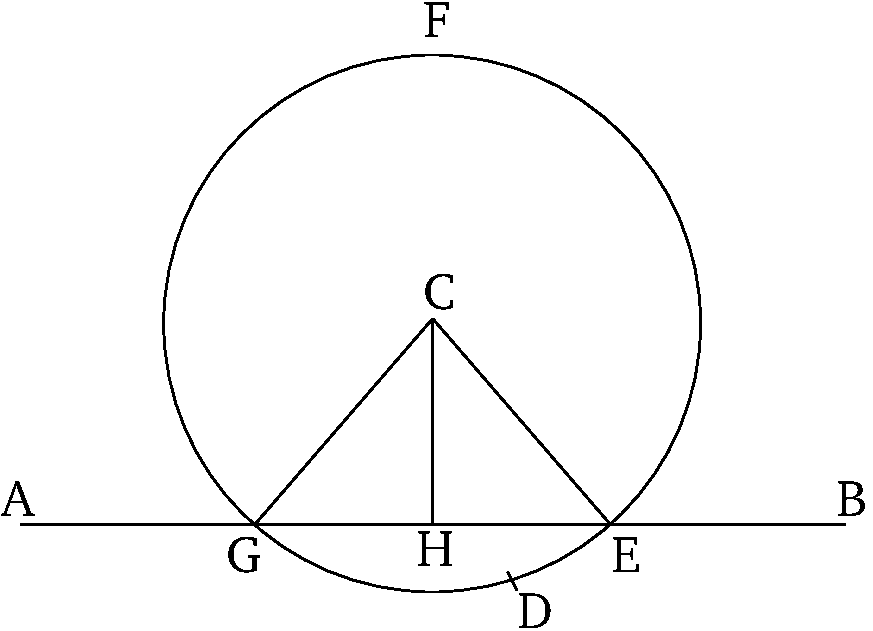
\includegraphics[width=0.8\textwidth]{Book01/fig12e.pdf}}

Let $AB$ be the given infinite straight-line  and $C$ the given point, which is not
on it. So it is required to draw a  straight-line  perpendicular to the
given infinite straight-line $AB$ from the given point $C$, which is not on
it.

For let point $D$ be taken at random on the other side (to $C$) of 
the straight-line $AB$, and let the circle $EFG$ be drawn
with center $C$ and radius $CD$ [Post.~3], and let the straight-line $EG$ be cut
in half at (point) $H$ [Prop.~1.10], and let the straight-lines $CG$, $CH$,
and $CE$ be joined. I say that the  (straight-line) $CH$ has
been drawn  perpendicular to the given infinite straight-line
$AB$ from the given point $C$, which is not on it.

For since $GH$ is equal to $HE$, and $HC$ (is) common, the two (straight-lines) $GH$, 
$HC$
are equal to the two (straight-lines) $EH$, $HC$, respectively, and the base $CG$ is
equal to the base $CE$. Thus, the angle $CHG$ is equal to the
angle $EHC$ [Prop.~1.8], and they are adjacent. But when a straight-line
stood on a(nother) straight-line makes the adjacent angles equal to one another, each of the equal angles is a right-angle, and the former straight-line is called a perpendicular to that upon which it stands [Def.~1.10].

Thus, the (straight-line) $CH$ has been drawn perpendicular to the given infinite straight-line $AB$ from the given point $C$, which is not
on  it. (Which is) the very thing it was required to do.}
\end{Parallel}

%%%%%%
% Prop 1.13
%%%%%%
\pdfbookmark[1]{Proposition 1.13}{pdf1.13}
\begin{Parallel}{}{} 
\ParallelLText{
\begin{center}
{\large\ggn{13}.}
\end{center}\vspace*{-7pt}

\gr{Ἐὰν εὐθεῖα ἐπ' εὐθεῖαν σταθεῖσα γωνίας ποιῆ|,  ἢτοι δύο ὀρθὰξὸὴ δυσὶν ὀρθαῖξ ἴσας ποιήσει.}

\gr{Εὐθεῖα γάρ τις ἡ ΑΒ ἐπ' εὐθεῖαν τὴν ΓΔ σταθεῖσα γωνίας ποιείτω
τὰξ ὑπὸ ΓΒΑ, ΑΒΔ; λὲγω, ὅτι αἱ ὑπὸ ΓΒΑ, ΑΒΔ γωνίαι ἢτοι
δύο ὀρθαί εἰσινὸὴ δυσὶν ὀρθαῖξ ἴσαι.}\\~\\

% Removed epsf size command
\centerline{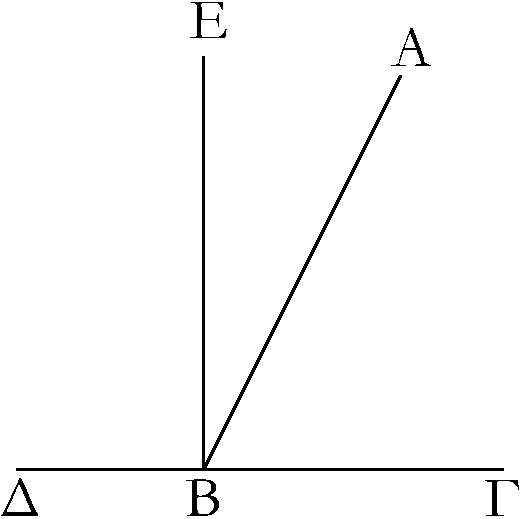
\includegraphics[width=0.8\textwidth]{Book01/fig13g.pdf}}

\gr{Εἰ μὲν οὸῦνὸίση ἐστὶν ἡ ὑπὸ ΓΒΑ τῇ ὑπὸ ΑΒΔ, δύο
ὀρθαί εἰσιν. εἰ δὲ οὸύ,  ἢθθω ἀπὸ τοῦ Β σημείου τῇ ΓΔ
[εὐθείᾳ] πρὸς ὀρθὰξ ἡ ΒΕ; αἱ  ἄρα ὑπὸ ΓΒΕ, ΕΒΔ δύο ὀρθαί
εἰσιν; καὶ ἐπεὶ ἡ ὑπὸ ΓΒΕ δυσὶ ταῖς ὑπὸ ΓΒΑ, ΑΒΕὸίση
ἐστίν, κοινὴ προσκείσθω ἡ ὑπὸ ΕΒΔ; αἱ  ἄρα ὑπὸ ΓΒΕ, ΕΒΔ
τρισὶ ταῖς ὑπὸ ΓΒΑ, ΑΒΕ, ΕΒΔ ἴσαι εἰσίν. πάλιν, ἐπεὶ ἡ ὑπὸ
ΔΒΑ δυσὶ ταῖς ὑπὸ ΔΒΕ, ΕΒΑὸίση ἐστίν, κοινὴ προσκείσθω
ἡ ὑπὸ ΑΒΓ; αἱ  ἄρα ὑπὸ ΔΒΑ, ΑΒΓ τρισὶ ταῖς ὑπὸ ΔΒΕ, ΕΒΑ, ΑΒΓ ἴσαι εἰσίν. ἐδείθθησαν δὲ καὶ αἱ ὑπὸ ΓΒΕ, ΕΒΔ τρισὶ
ταῖς αὐταῖς ἴσαι; τὰ δὲ τῷ αὐτῷ  ἴσα καὶ ἀλλήλοις ἐστὶν ἴσα;
 καὶ αἱ ὑπὸ ΓΒΕ, ΕΒΔ ἄρα ταῖς ὑπὸ ΔΒΑ, ΑΒΓ ἴσαι εἰσίν; ἀλλὰ αἱ ὑπὸ ΓΒΕ, ΕΒΔ δύο
ὀρθαί εἰσιν; καὶ αἱ ὑπὸ ΔΒΑ, ΑΒΓ ἄρα δυσὶν ὀρθαῖξ ἴσαι εἰσίν.}

\gr{Ἐὰν ἄρα εὐθεῖα ἐπ' εὐθεῖαν σταθεῖσα γωνίας ποιῆ|,  ἢτοι δύο ὀρθὰξὸὴ δυσὶν ὀρθαῖξ ἴσας ποιήσει; ὅπερ ἔδει δεῖχαι.}}

\ParallelRText{
\begin{center}
{\large Proposition 13}
\end{center}

If a straight-line stood on a(nother)  straight-line makes angles,
it will certainly either make two right-angles, or (angles whose sum is) equal
to two right-angles. 

For  let some straight-line $AB$ stood on the straight-line $CD$ make the
angles $CBA$ and $ABD$. I say that the angles $CBA$ and $ABD$ are
certainly either two right-angles, or (have a sum) equal to two right-angles.

% Removed epsf size command
\centerline{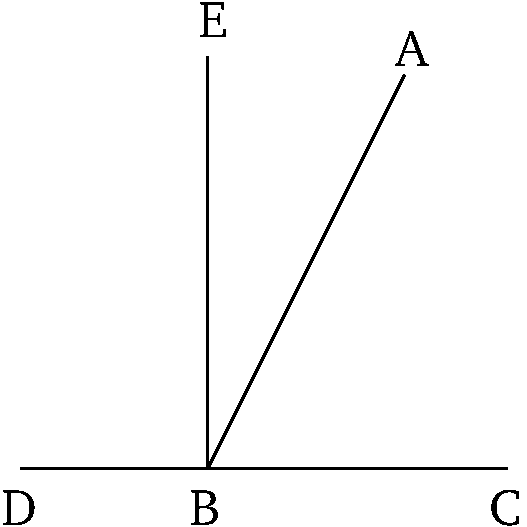
\includegraphics[width=0.8\textwidth]{Book01/fig13e.pdf}}

In fact, if $CBA$ is equal to $ABD$ (then) they are two right-angles [Def.~1.10].
But, if not, let $BE$ be drawn from the point $B$ at right-angles to [the
straight-line] $CD$ [Prop.~1.11]. Thus, $CBE$ and $EBD$ are two right-angles.
And since $CBE$ is equal to the two (angles) $CBA$ and $ABE$, let $EBD$ be added
to both. Thus, the (sum of the angles) $CBE$ and $EBD$ is equal to the  (sum of the) three (angles)
$CBA$, $ABE$, and $EBD$ [C.N.~2]. Again, since $DBA$ is equal to the two (angles) $DBE$
and $EBA$, let $ABC$ be added to both. Thus, the (sum of the angles) $DBA$ and $ABC$ is
equal to the (sum of the) three (angles) $DBE$, $EBA$, and $ABC$ [C.N.~2]. But (the sum of) $CBE$ and $EBD$ was
also shown (to be) equal to the (sum of the) same three (angles). And things equal to the
same thing are also equal to one another [C.N.~1]. Therefore, 
(the sum of) $CBE$ and
$EBD$ is also equal to (the sum of) $DBA$ and $ABC$. But, (the sum of) $CBE$ and $EBD$ is two
right-angles. Thus, (the sum of) $ABD$ and $ABC$ is also equal to two right-angles.

Thus, if a straight-line stood on a(nother)  straight-line makes angles,
it will certainly either make two right-angles, or (angles whose sum is) equal
to two right-angles. (Which is) the very thing it was required to show.}
\end{Parallel}

%%%%%%
% Prop 1.14
%%%%%%
\pdfbookmark[1]{Proposition 1.14}{pdf1.14}
\begin{Parallel}{}{} 
\ParallelLText{
\begin{center}
{\large \ggn{14}.}
\end{center}\vspace*{-7pt}

\gr{Ἐὰν πρόξ τινι εὐθείᾳ καὶ τῷ πρὸς αὐτῇ σημείῳ δύο εὐθεῖαι
μὴ ἐπὶ τὰ αὐτὰ μέρη κείμεναι τὰξ ἐφεχῆς γωνίας δυσὶν ὀρθαῖξ ἴσας ποιῶσιν, ἐπ' εὐθείαςὸέσονται ἀλλήλαις αἱ εὐθεῖαι.}

\gr{Πρὸξ γάρ τινι εὐθείᾳ τῇ ΑΒ καὶ τῷ πρὸς αὐτῇ σημείῳ τῷ
Β δύο εὐθεῖαι αἱ ΒΓ, ΒΔ μὴ ἐπὶ τὰ αὐτὰ μέρη
κείμεναι
τὰξ ἐφεχῆς γωνίας τὰξ ὑπὸ ΑΒΓ, ΑΒΔ δύο ὀρθαῖξ ἴσας ποιείτωσαν; λέγω, ὅτι ἐπ' εὐθείας ἐστὶ τῇ ΓΒ ἡ ΒΔ.}\\

% Removed epsf size command
\centerline{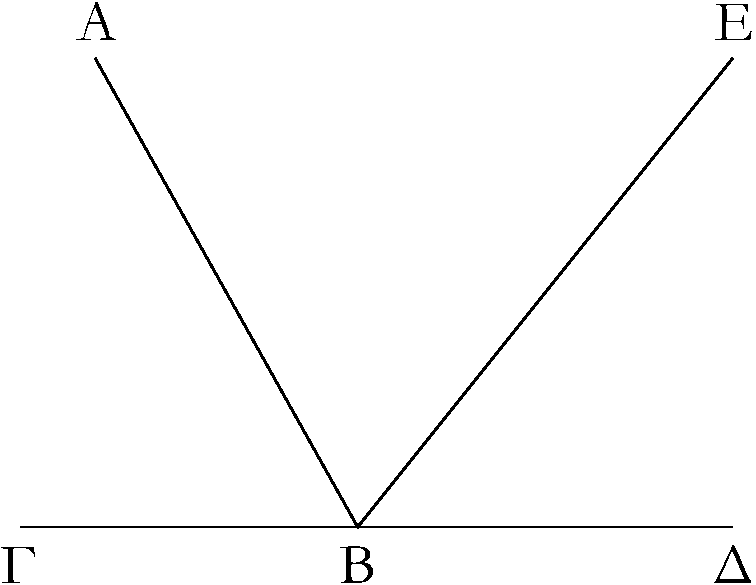
\includegraphics[width=0.8\textwidth]{Book01/fig14g.pdf}}

\gr{Εἰ γὰρ μή ἐστι τῇ ΒΓ ἐπ' εὐθείας ἡ ΒΔ, ὸέστω τῇ ΓΒ ἐπ'
εὐθείας ἡ ΒΕ.}

\gr{Ἐπεὶ οὸῦν εὐθεῖα ἡ ΑΒ ἐπ' εὐθεῖαν τὴν ΓΒΕ ἐφέστηκεν, αἱ
 ἄρα ὑπὸ ΑΒΓ, ΑΒΕ γωνίαι δύο ὀρθαῖξ ἴσαι εἰσίν; εἰσὶ δὲ καὶ
αἱ ὑπὸ ΑΒΓ, ΑΒΔ δύο ὀρθαῖξ ἴσαι; αἱ  ἄρα ὑπὸ ΓΒΑ, ΑΒΕ
ταῖς ὑπὸ ΓΒΑ, ΑΒΔ ἴσαι εἰσίν. κοινὴ ἀφῃρήσθω ἡ ὑπὸ ΓΒΑ;
λοιπὴ  ἄρα ἡ ὑπὸ ΑΒΕ λοιπῆ| τῇ ὑπὸ ΑΒΔ ἐστινὸίση, ἡ
ἐλάσσων τῇ μείζονι; ὅπερ ἐστὶν ἀδύνατον. οὐκ ἄρα
ἐπ' εὐθείας ἐστὶν ἡ ΒΕ τῇ ΓΒ. ὁμοίως δὴ δείχομεν, ὅτι
οὐδὲ ὸάλλη τις πλὴν τῆς ΒΔ; ἐπ' εὐθείας ἄρα ἐστὶν ἡ ΓΒ τῇ ΒΔ.}

\gr{Ἐὰν ἄρα πρόξ τινι εὐθείᾳ καὶ τῷ πρὸς αὐτῇ σημείῳ δύο εὐθεῖαι
μὴ ἐπὶ αὐτὰ μέρη κείμεναι τὰξ ἐφεχῆς γωνίας δυσὶν ὀρθαῖξ ἴσας ποιῶσιν, ἐπ' εὐθείαςὸέσονται ἀλλήλαις αἱ εὐθεῖαι; ὅπερ ἔδει δεῖχαι.}}

\ParallelRText{
\begin{center}
{\large Proposition 14}
\end{center}

If two straight-lines, not lying on the same side,  make adjacent angles (whose sum is) equal to two right-angles  with some straight-line, at a point on it, (then) the two straight-lines
will be straight-on (with respect) to one another.

For let two
straight-lines $BC$ and $BD$, not lying on the same side,  make adjacent angles $ABC$ and $ABD$ (whose sum is)
equal to two right-angles with some straight-line $AB$, at the point $B$ on it. I say
that $BD$ is  straight-on with respect to $CB$.

% Removed epsf size command
\centerline{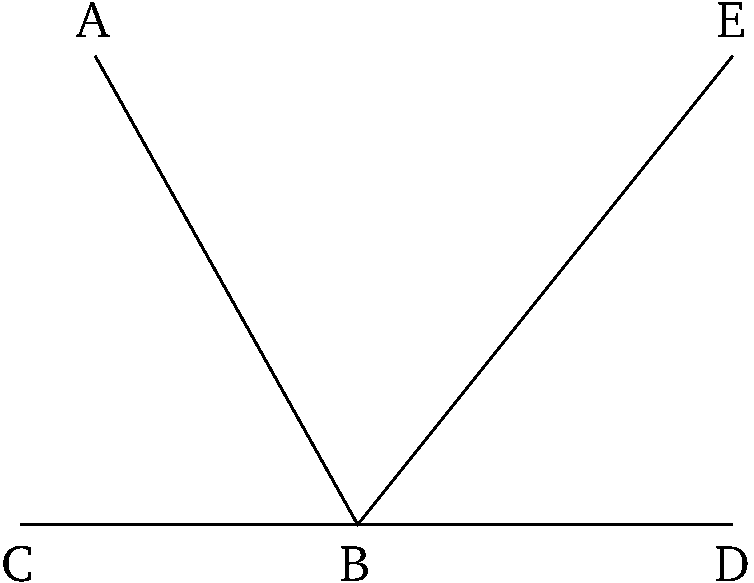
\includegraphics[width=0.8\textwidth]{Book01/fig14e.pdf}}

For if $BD$ is not straight-on to $BC$ (then) let $BE$ be straight-on to $CB$.

Therefore, since the straight-line $AB$ stands on the straight-line $CBE$, the (sum of the) angles $ABC$ and $ABE$ is thus equal to two right-angles [Prop.~1.13]. But (the sum of) $ABC$ and $ABD$ is also equal to two right-angles.
Thus, 
(the sum of angles) $CBA$ and $ABE$ is equal to (the sum of angles) $CBA$ and $ABD$ [C.N.~1]. Let (angle)
$CBA$ be subtracted from both. Thus, the remainder $ABE$ is
equal to the remainder $ABD$ [C.N.~3], the lesser to the greater. The very thing is impossible. Thus, $BE$ is not straight-on with respect to $CB$. Similarly, we can
show that neither (is) any other (straight-line)   than $BD$.
Thus, $CB$ is straight-on with respect to $BD$.

Thus, if two straight-lines, not lying on the same side,  make adjacent angles (whose sum is) equal to two right-angles with some straight-line, at a point on it, (then) the two straight-lines
will be straight-on (with respect) to one another. (Which is) the very thing it
was required to show.}
\end{Parallel}

%%%%%%
% Prop 1.15
%%%%%%
\pdfbookmark[1]{Proposition 1.15}{pdf1.15}
\begin{Parallel}{}{} 
\ParallelLText{
\begin{center}
{\large \ggn{15}.}
\end{center}\vspace*{-7pt}

\gr{Ἐὰν δύο εὐθεῖαι τέμνωσιν ἀλλήλας, τὰξ κατὰ κορυφὴν γωνίας ἴσας ἀλλήλαις ποιοῦσιν.}

\gr{Δύο γὰρ εὐθεῖαι αἱ ΑΒ, ΓΔ τεμνέτωσαν ἀλλήλας κατὰ τὸ Ε σημεῖον;
λέγω, ὅτιὸίση ἐστὶν ἡ μὲν ὑπὸ ΑΕΓ γωνία τῇ ὑπὸ ΔΕΒ, ἡ
δὲ ὑπὸ ΓΕΒ τῇ ὑπὸ ΑΕΔ.}

% Removed epsf size command
\centerline{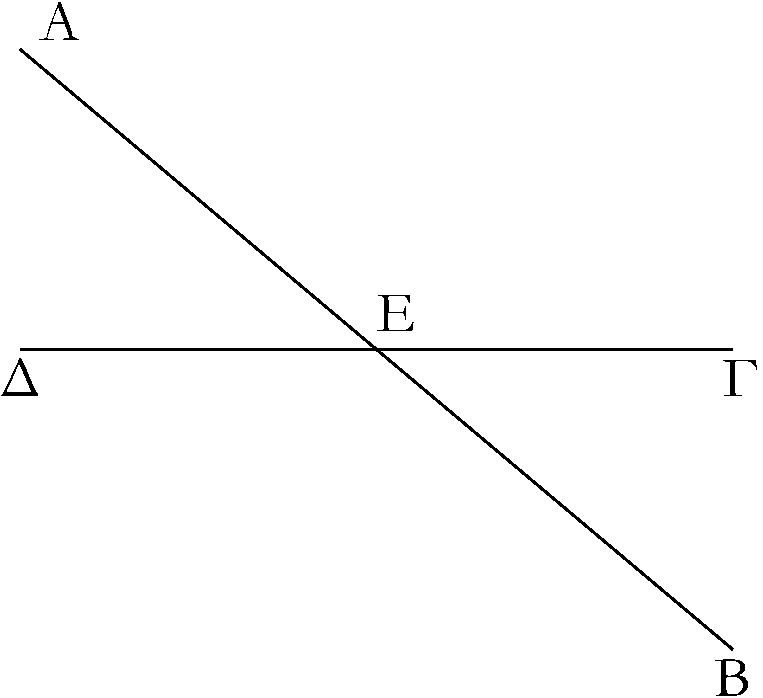
\includegraphics[width=0.8\textwidth]{Book01/fig15g.pdf}}

\gr{Ἐπεὶ γὰρ εὐθεῖα ἡ ΑΕ ἐπ' εὐθεῖαν τὴν ΓΔ ἐφέστηκε γωνίας ποιοῦσα τὰξ ὑπὸ ΓΕΑ, ΑΕΔ, αἱ  ἄρα ὑπὸ ΓΕΑ, ΑΕΔ γωνίαι δυσὶν
ὀρθαῖξ ἴσαι εἰσίν. πάλιν, ἐπεὶ εὐθεῖα ἡ ΔΕ ἐπ' εὐθεῖαν
τὴν ΑΒ ἐφέστηκε γωνίας ποιοῦσα τὰξ ὑπὸ ΑΕΔ, ΔΕΒ, αἱ  ἄρα
ὑπὸ ΑΕΔ, ΔΕΒ γωνίαι δυσὶν ὀρθαῖξ ἴσαι εἰσίν. ἐδείθθησαν
δὲ καὶ αἱ ὑπὸ ΓΕΑ, ΑΕΔ δυσὶν ὀρθαῖξ ἴσαι; αἱ  ἄρα ὑπὸ ΓΕΑ,
ΑΕΔ ταῖς ὑπὸ ΑΕΔ, ΔΕΒ ἴσαι εἰσίν. κοινὴ ἀφῃρήσθω ἡ ὑπὸ
ΑΕΔ; λοιπὴ  ἄρα ἡ ὑπὸ ΓΕΑ λοιπῆ| τῇ ὑπὸ ΒΕΔὸίση ἐστίν;
ὁμοίως δὴ δειθθήσεται, ὅτι καὶ αἱ ὑπὸ ΓΕΒ, ΔΕΑ ἴσαι εἰσίν.}

\gr{Ἐὰν ἄρα δύο εὐθεῖαι τέμνωσιν ἀλλήλας, τὰξ κατὰ κορυφὴν γωνίας ἴσας ἀλλήλαις ποιοῦσιν; ὅπερ ἔδει δεῖχαι.}}

\ParallelRText{
\begin{center}
{\large Proposition 15}
\end{center}

If two straight-lines cut one another (then) they make the vertically opposite angles
equal to one another.

For let the two straight-lines $AB$ and $CD$ cut one another at the point $E$. I say
that  angle $AEC$ is equal to (angle) $DEB$, and (angle) $CEB$ to (angle) $AED$.

% Removed epsf size command
\centerline{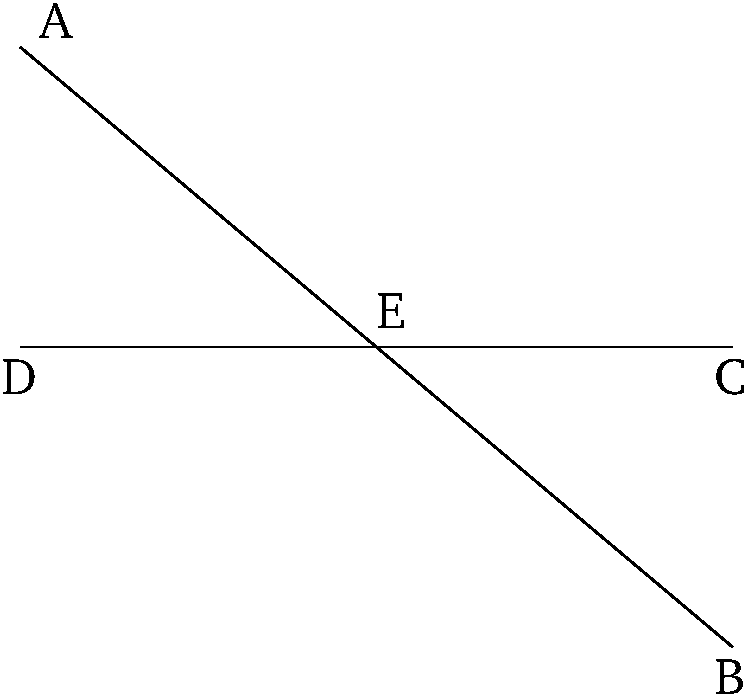
\includegraphics[width=0.8\textwidth]{Book01/fig15e.pdf}}

For since the straight-line $AE$ stands on the straight-line $CD$, making the
angles $CEA$ and $AED$, the (sum of the) angles $CEA$ and $AED$ is thus equal to two
right-angles [Prop.~1.13]. Again, since the straight-line $DE$ stands on the
straight-line $AB$, making the angles $AED$ and $DEB$, the (sum of the) angles $AED$ and
$DEB$ is thus equal to two right-angles [Prop.~1.13]. But (the sum of) $CEA$ and $AED$ was also shown
(to be) equal to two right-angles. Thus, (the sum of) $CEA$ and $AED$ is equal to (the sum of) $AED$ and $DEB$ [C.N.~1]. Let $AED$ be subtracted from both. Thus, the remainder
$CEA$ is equal to the remainder $BED$ [C.N.~3]. Similarly, it can be shown that
$CEB$ and $DEA$ are also equal.

Thus, if two straight-lines cut one another (then) they make the vertically opposite angles
equal to one another. (Which is) the very thing it was required to show.}
\end{Parallel}

%%%%%%
% Prop 1.16
%%%%%%
\pdfbookmark[1]{Proposition 1.16}{pdf1.16}
\begin{Parallel}{}{} 
\ParallelLText{
\begin{center}
{\large \ggn{16}.}
\end{center}\vspace*{-7pt}

\gr{Παντὸξ τριγώνου μιᾶς τῶν πλευρῶν προσεκβληθείσης ἡ ἐκτὸξ γωνία
ἑκατέρας τῶν ἐντὸς καὶ ἀπεναντίον γωνιῶν μείζων ἐστίν.}

\gr{Ἔστω τρίγωνον τὸ ΑΒΓ, καὶ προσεκβεβλήσθω αὐτοῦ μία πλευρὰ
ἡ ΒΓ ἐπὶ τὸ Δ; λὲγω, ὅτι ἡ ἐκτὸξ γωνία ἡ ὑπὸ ΑΓΔ
μείζων ἐστὶν ἑκατέρας τῶν ἐντὸς καὶ ἀπεναντίον τῶν
ὑπὸ ΓΒΑ, ΒΑΓ γωνιῶν.}

\gr{Τετμήσθω ἡ ΑΓ δίθα κατὰ τὸ Ε, καὶ ἐπιζευθθεῖσα ἡ ΒΕ ἐκβεβλήσθω
ἐπ' εὐθείας ἐπὶ τὸ Ζ, καὶ κείσθω τῇ ΒΕὸίση ἡ ΕΖ, καὶ ἐπεζεύθθω
ἡ ΖΓ, καὶ διήθθω ἡ ΑΓ ἐπὶ τὸ Η.}\\

% Removed epsf size command
\centerline{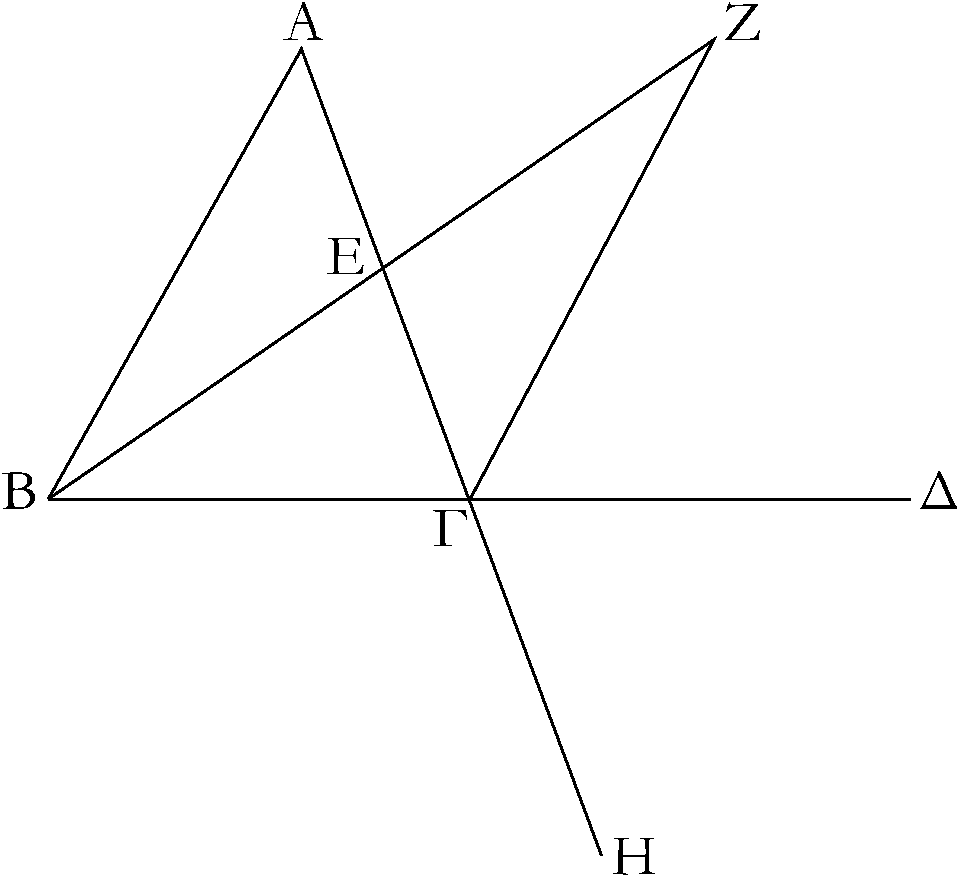
\includegraphics[width=0.8\textwidth]{Book01/fig16g.pdf}}

\gr{Ἐπεὶ οὸῦνὸίση ἐστὶν ἡ μὲν ΑΕ τῇ ΕΓ, ἡ δὲ ΒΕ τῇ ΕΖ, δύο
δὴ αἱ ΑΕ, ΕΒ δυσὶ ταῖς ΓΕ, ΕΖ ἴσαι εἰσὶν ἑκατέρα ἑκατέρᾳ;
καὶ γωνία ἡ ὑπὸ ΑΕΒ γωνίᾳ τῇ ὑπὸ ΖΕΓὸίση ἐστίν; κατὰ κορυφὴν γάρ; βάσις ἄρα ἡ ΑΒ βάσει τῇ ΖΓὸίση ἐστίν, καὶ τὸ ΑΒΕ
τρίγωνον τῷ ΖΕΓ τριγώνῳ ἐστὶν ἴσον, καὶ αἱ λοιπαὶ
γωνίαι ταῖς λοιπαῖξ γωνίαις ἴσαι εἰσὶν ἑκατέρα
 ἑκατέρᾳ,
ὑφὸ ὁὰξ αἱ  ἴσαι πλευραὶ ὑποτείνουσιν; ὸίση ἄρα ἐστὶν ἡ
ὑπὸ ΒΑΕ τῇ ὑπὸ ΕΓΖ. μείζων δέ ἐστιν ἡ ὑπὸ ΕΓΔ τῆς
ὑπὸ ΕΓΖ; μείζων ἄρα ἡ ὑπὸ ΑΓΔ τῆς ὑπὸ ΒΑΕ. Ὁμοίως
δὴ τῆς ΒΓ τετμ  ημένης δίθα δειθθήσεται καὶ ἡ ὑπὸ ΒΓΗ, τουτέστιν
ἡ ὑπὸ ΑΓΔ, μείζων καὶ τῆς ὑπὸ ΑΒΓ.}

\gr{Παντὸξ ἄρα τριγώνου μιᾶς τῶν πλευρῶν προσεκβληθείσης ἡ ἐκτὸξ γωνία
ἑκατέρας τῶν ἐντὸς καὶ ἀπεναντίον γωνιῶν μείζων ἐστίν;
ὅπερ ἔδει δεῖχαι.}}

\ParallelRText{
\begin{center}
{\large Proposition 16}
\end{center}

For any triangle, when one of the sides is produced, the external angle
is greater than each of the internal and opposite angles.

Let $ABC$ be a triangle, and let one of its sides $BC$ be produced 
 to $D$. I say that the external angle $ACD$ is greater than each of the
 internal and opposite angles, $CBA$ and $BAC$.
 
 Let the (straight-line) $AC$ be cut in half at (point) $E$ [Prop.~1.10].
 And $BE$ being joined, let it be produced in a straight-line to
 (point) $F$.$^\dag$ And let $EF$ be made equal to $BE$ [Prop.~1.3], and let $FC$ be joined, and let $AC$ be drawn through to (point) $G$.
 
% Removed epsf size command
\centerline{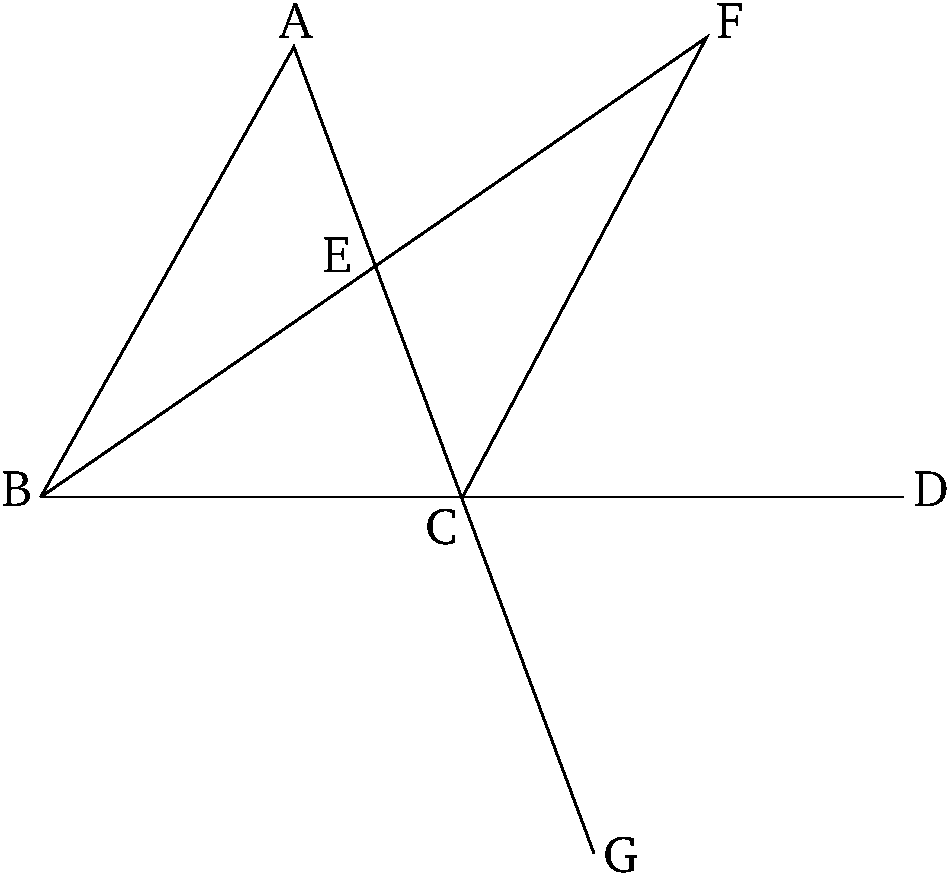
\includegraphics[width=0.8\textwidth]{Book01/fig16e.pdf}}

 Therefore, since $AE$ is equal to $EC$, and $BE$ to $EF$, the two (straight-lines)
 $AE$, $EB$ are equal to the two (straight-lines) $CE$, $EF$, respectively. 
 Also, angle $AEB$ is equal to angle $FEC$, for (they are)
 vertically opposite [Prop.~1.15]. Thus, the base $AB$ is equal to the base
 $FC$, and the triangle $ABE$ is equal to the triangle $FEC$, and the remaining
 angles subtended by the equal sides are equal to the corresponding remaining angles [Prop.~1.4]. Thus, $BAE$ is equal to $ECF$. But $ECD$ is greater than $ECF$. Thus,
 $ACD$ is greater than $BAE$. Similarly, by having cut $BC$ in half,  it can  be shown (that) $BCG$---that is to say, $ACD$---(is) also greater than $ABC$.
 
 Thus, for any triangle, when one of the sides is produced, the external angle
is greater than each of the internal and opposite angles. (Which is) the very thing
it was required to show.}
\end{Parallel}
{\footnotesize
\noindent $^\dag$  The implicit assumption that the point $F$ lies in the
 interior of the angle $ABC$ should be counted as an additional postulate.} 
 
 %%%%%%
% Prop 1.17
%%%%%%
\pdfbookmark[1]{Proposition 1.17}{pdf1.17}
\begin{Parallel}{}{} 
\ParallelLText{
\begin{center}
{\large \ggn{17}.}
\end{center}\vspace*{-7pt}

\gr{Παντὸνς τριγώνου αἱ δύο γωνίαι δύο ὀρθῶν ἐλάσσονέξ εἰσι πάντῇ μεταλαμβανόμεναι.}

\gr{Ἔστω τρίγωνον τὸ ΑΒΓ; λέγω, ὅτι τοῦ ΑΒΓ τριγώνου αἱ δύο γωνίαι δύο ὀρθῶν ἐλάττονέξ εἰσι πάντῃ μεταλαμβανόμεναι.}

\gr{Ἐκβεβλήσθω γὰρ ἡ ΒΓ ἐπὶ τὸ Δ.}

\gr{Καὶ ἐπεὶ τριγώνου τοῦ ΑΒΓ ἐκτόξ ἐστι γωνία ἡ ὑπὸ ΑΓΔ,
μείζων ἐστὶ τῆς ἐντὸς καὶ ἀπεναντίον τῆς ὑπὸ ΑΒΓ. κοινὴ
προσκείσθω ἡ ὑπὸ ΑΓΒ; αἱ  ἄρα ὑπὸ ΑΓΔ, ΑΓΒ τῶν ὑπὸ ΑΒΓ,
ΒΓΑ μείζονέξ εἰσιν. ἀλλὸ  αἱ ὑπὸ ΑΓΔ, ΑΓΒ δύο ὀρθαῖξ ἴσαι εἰσίν; αἱ  ἄρα ὑπὸ  
ΑΒΓ, ΒΓΑ δύο ὀρθῶν ἐλάσσονέξ εἰσιν.
ὁμοίως δὴ δείχομεν, ὅτι καὶ αἱ ὑπὸ ΒΑΓ, ΑΓΒ δύο
ὀρθῶν ἐλάσσονέξ εἰσι καὶ ὸέτι αἱ ὑπὸ
ΓΑΒ, ΑΒΓ.}\\~\\~\\

% Removed epsf size command
\centerline{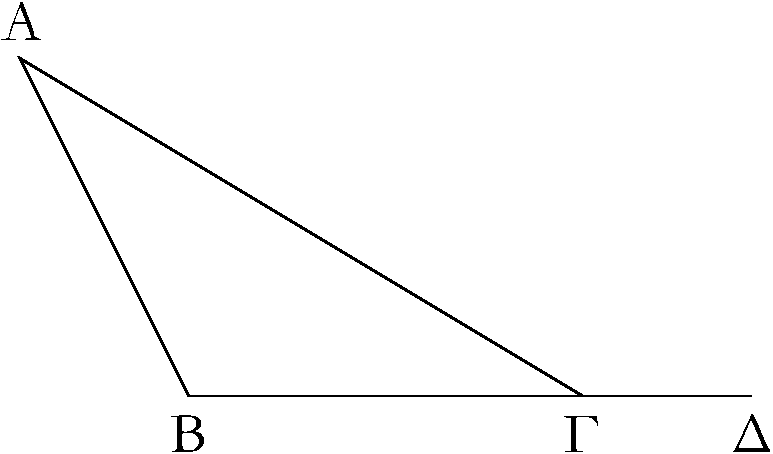
\includegraphics[width=0.8\textwidth]{Book01/fig17g.pdf}}

\gr{Παντὸνς ἄρα τριγώνου αἱ δύο γωνίαι δύο ὀρθῶν ἐλάσσονέξ εἰσι πάντῇ μεταλαμβανόμεναι; ὅπερ ἔδει δεῖχαι.}}

\ParallelRText{
\begin{center}
{\large Proposition 17}
\end{center}

For any triangle,  (the sum of) two angles taken together in any (possible way) is less than two right-angles.

Let $ABC$ be a triangle. I say that (the sum of) two angles of triangle $ABC$
taken together in any (possible way) is less than two right-angles.

For let $BC$ be produced to $D$.

And since the angle $ACD$ is external to triangle $ABC$, it is greater than the
internal and opposite angle $ABC$ [Prop.~1.16]. Let $ACB$ be added to both. Thus, the
(sum of the angles) $ACD$ and $ACB$ is greater than the  (sum of the angles) $ABC$ and
$BCA$. But, (the sum of) $ACD$ and $ACB$ is equal to two right-angles [Prop.~1.13].
Thus, (the sum of) $ABC$ and $BCA$ is less than two right-angles. Similarly,
we can show that (the sum of) $BAC$ and $ACB$ is also less than two right-angles,
and further (that the sum of) $CAB$ and $ABC$ (is less than two right-angles).

% Removed epsf size command
\centerline{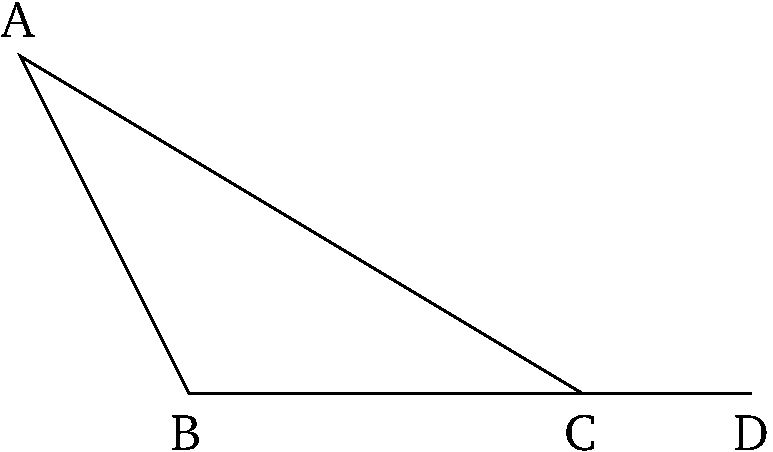
\includegraphics[width=0.8\textwidth]{Book01/fig17e.pdf}}

Thus, for any triangle,  (the sum of) two angles taken together in any (possible way) is less than two right-angles. (Which is) the very thing
it was required to show.}
\end{Parallel}

%%%%%%
% Prop 1.18
%%%%%%
\pdfbookmark[1]{Proposition 1.18}{pdf1.18}
\begin{Parallel}{}{} 
\ParallelLText{
\begin{center}
{\large \ggn{18}.}
\end{center}\vspace*{-7pt}

\gr{Παντὸξ τριγώνου ἡ μείζων πλευρὰ τὴν μείζονα γωνίαν ὑποτείνει.}

\gr{Ἔστω γὰρ τρίγωνον τὸ ΑΒΓ μείζονα ἔχον τὴν ΑΓ πλευρὰν τῆς
ΑΒ; λέγω, ὅτι καὶ γωνία ἡ ὑπὸ ΑΒΓ μείζων ἐστὶ τῆς ὑπὸ ΒΓΑ.}

% Removed epsf size command
\centerline{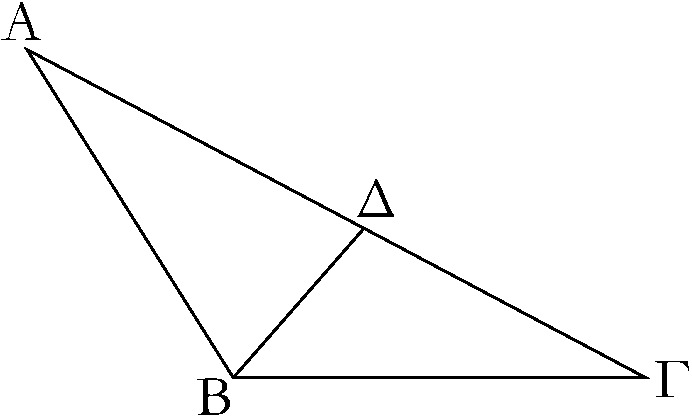
\includegraphics[width=0.8\textwidth]{Book01/fig18g.pdf}}

\gr{Ἐπεὶ γὰρ μείζων ἐστὶν ἡ ΑΓ τῆς ΑΒ, κείσθω τῇ ΑΒὸίση ἡ
ΑΔ, καὶ ἐπεζεύθθω ἡ ΒΔ.}

\gr{Καὶ ἐπεὶ τριγώνου τοῦ ΒΓΔ ἐκτόξ ἐστι γωνία ἡ ὑπὸ ΑΔΒ,
μείζων ἐστὶ τῆς ἐντὸς καὶ ἀπεναντίον τῆς ὑπὸ ΔΓΒ; ὸίση
δὲ ἡ ὑπὸ ΑΔΒ τῇ ὑπὸ ΑΒΔ, ἐπεὶ καὶ πλευρὰ ἡ ΑΒ τῇ
ΑΔ ἐστινὸίση; μείζων ἄρα καὶ ἡ ὑπὸ ΑΒΔ τῆς ὑπὸ ΑΓΒ;
πολλῶ|  ἄρα ἡ ὑπὸ ΑΒΓ μείζων ἐστὶ τῆς ὑπὸ ΑΓΒ.}

\gr{Παντὸξ ἄρα τριγώνου ἡ μείζων πλευρὰ τὴν μείζονα γωνίαν
ὑποτείνει; ὅπερ ἔδει δεῖχαι.}}

\ParallelRText{
\begin{center}
{\large Proposition 18}
\end{center}

In any triangle, the greater side subtends the greater angle.

For let $ABC$ be a triangle having side $AC$ greater than $AB$. I say that
angle $ABC$ is also greater than $BCA$.\\~\\

% Removed epsf size command
\centerline{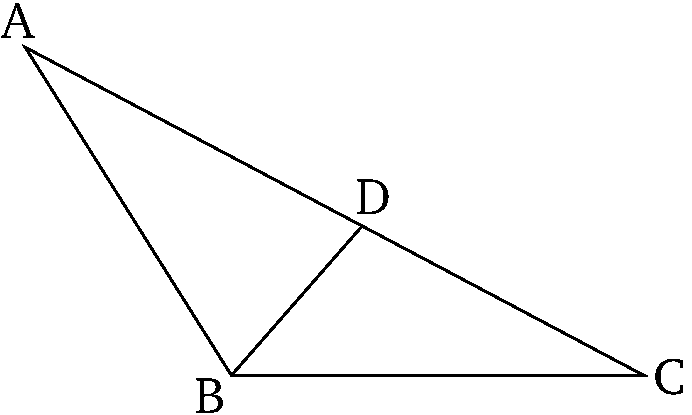
\includegraphics[width=0.8\textwidth]{Book01/fig18e.pdf}}

For since $AC$ is greater than $AB$, let $AD$ be made equal to $AB$
 [Prop.~1.3],
and let $BD$ be joined.

And since angle $ADB$ is external to triangle $BCD$, it is greater than the
internal and opposite (angle) $DCB$ [Prop.~1.16]. But $ADB$ (is) equal to $ABD$,
since side $AB$ is also equal to side $AD$ [Prop.~1.5]. Thus,
$ABD$ is also greater than $ACB$. Thus, $ABC$ is much greater than 
$ACB$.

Thus, in any triangle, the greater side subtends the greater angle.
(Which is) the very thing  it was required to show.}
\end{Parallel}

%%%%%%
% Prop 1.19
%%%%%%
\pdfbookmark[1]{Proposition 1.19}{pdf1.19}
\begin{Parallel}{}{} 
\ParallelLText{
\begin{center}
{\large \ggn{19}.}
\end{center}\vspace*{-7pt}

\gr{Παντὸξ τριγώνου ὑπὸ τὴν μείζονα γωνίαν ἡ μείζων πλευρὰ ὑποτείνει.}

\gr{Ἔστω τρίγωνον τὸ ΑΒΓ  μείζονα ἔχον τὴν ὑπὸ ΑΒΓ γωνίαν τῆς ὑπὸ ΒΓΑ; λέγω, ὅτι καὶ πλευρὰ ἡ ΑΓ πλευρᾶξ τῆς ΑΒ μείζων
ἐστίν.}

% Removed epsf size command
\centerline{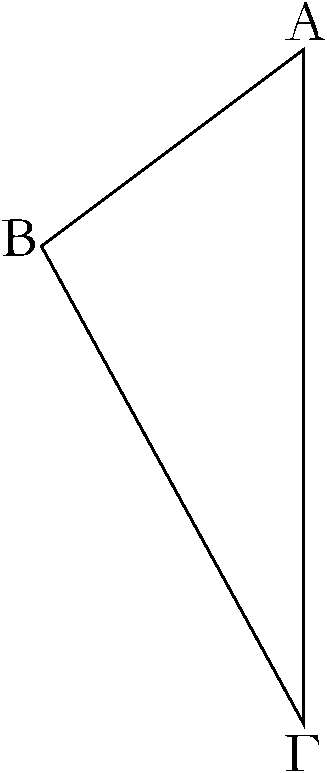
\includegraphics[width=0.8\textwidth]{Book01/fig19g.pdf}}

\gr{ Εἰ γὰρ μή,  ἢτοιὸίση ἐστὶν ἡ ΑΓ τῇ ΑΒὸὴ ἐλάσσων; ὸίση μὲν οὸῦν οὐκὸέστιν ἡ ΑΓ τῇ ΑΒ; ὸίση γὰρὸὰνὸῆν καὶ γωνία ἡ ὑπὸ
ΑΒΓ τῇ ὑπὸ ΑΓΒ; οὐκὸέστι δέ; οὐκ ἄραὸίση ἐστὶν ἡ ΑΓ
τῇ ΑΒ. οὐδὲ μὴν ἐλάσσων ἐστὶν ἡ ΑΓ τῆς ΑΒ;
ἐλάσσων γὰρὸὰνὸῆν καὶ γωνία ἡ ὑπὸ ΑΒΓ τῆς ὑπὸ
ΑΓΒ; οὐκὸέστι δέ; οὐκ ἄρα ἐλάσσων ἐστὶν ἡ ΑΓ τῆς
ΑΒ. ἐδείθθη δέ, ὅτι οὐδὲ ὸίση ἐστίν. μείζων ἄρα ἐστὶν
ἡ ΑΓ τῆς ΑΒ.}

\gr{Παντὸξ ἄρα τριγώνου ὑπὸ τὴν μείζονα γωνίαν ἡ μείζων πλευρὰ ὑποτείνει; ὅπερ ἔδει δεῖχαι.}}

\ParallelRText{
\begin{center}
{\large Proposition 19}
\end{center}

In any triangle, the greater angle is subtended by the greater side.

Let $ABC$ be a triangle having the angle $ABC$ greater than $BCA$. I say
that side $AC$ is also greater than side $AB$.\\

% Removed epsf size command
\centerline{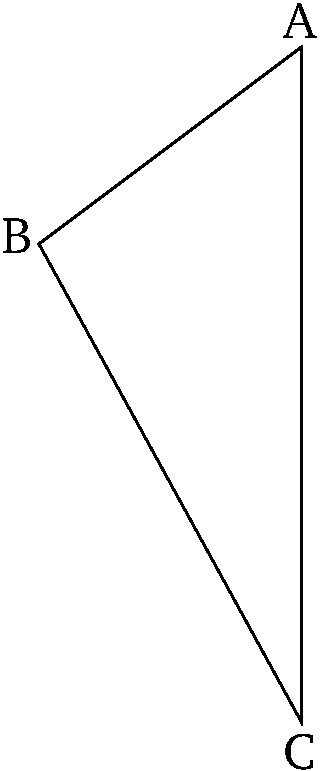
\includegraphics[width=0.8\textwidth]{Book01/fig19e.pdf}}

For if not, $AC$ is certainly either equal to, or less than, $AB$. In fact, $AC$ is not
equal to $AB$. For then angle $ABC$  would also be equal to $ACB$ [Prop.~1.5].
But it is not. Thus, $AC$ is not equal to $AB$.
Neither, indeed, is $AC$ less than $AB$. For then angle $ABC$ would also be
less than $ACB$ [Prop.~1.18]. But it is not. Thus, $AC$ is not less than
$AB$. But it was  shown that ($AC$) is    not equal (to $AB$) either. Thus, $AC$ 
is greater than $AB$.

Thus, in any triangle, the greater angle is subtended by the greater side.
(Which is) the very thing it was required to show.}
\end{Parallel}

%%%%%%
% Prop 1.20
%%%%%%
\pdfbookmark[1]{Proposition 1.20}{pdf1.20}
\begin{Parallel}{}{} 
\ParallelLText{
\begin{center}
{\large \ggn{20}.}
\end{center}\vspace*{-7pt}

\gr{Παντὸξ τριγώνου αἱ δύο πλευραὶ τῆς λοιπῆς μείζονέξ εἰσι πάντῃ
μεταλαμβανόμεναι.}

% Removed epsf size command
\centerline{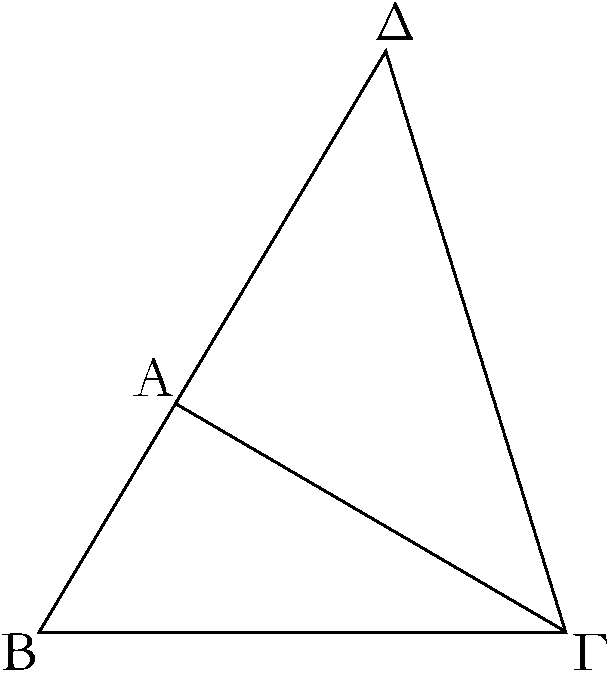
\includegraphics[width=0.8\textwidth]{Book01/fig20g.pdf}}

\gr{Ἔστω γὰρ τρίγωνον τὸ ΑΒΓ; λέγω, ὅτι τοῦ ΑΒΓ τριγώνου αἱ
δύο πλευραὶ τῆς λοιπῆς μείζονέξ εἰσι πάντῃ μεταλαμβανόμεναι,
αἱ μὲν ΒΑ, ΑΓ τῆς ΒΓ, αἱ δὲ ΑΒ, ΒΓ τῆς ΑΓ, αἱ δὲ ΒΓ, ΓΑ
τῆς ΑΒ.}

\gr{Διήθθω γὰρ ἡ ΒΑ ἐπὶ τὸ Δ σημεῖον, καὶ κείσθω τῇ
ΓΑὸίση ἡ ΑΔ, καὶ ἐπεζεύθθω ἡ ΔΓ.}

\gr{Ἐπεὶ οὸῦνὸίση ἐστὶν ἡ ΔΑ τῇ ΑΓ, ὸίση ἐστὶ καὶ
γωνία ἡ ὑπὸ ΑΔΓ τῇ ὑπὸ ΑΓΔ; μείζων ἄρα ἡ
ὑπὸ ΒΓΔ τῆς ὑπὸ ΑΔΓ; καὶ ἐπεὶ τρίγωνόν ἐστι τὸ ΔΓΒ
μείζονα ἔχον τὴν ὑπὸ ΒΓΔ γωνίαν τῆς ὑπὸ ΒΔΓ, ὑπὸ
δὲ τὴν μείζονα γωνίαν ἡ μείζων πλευρὰ ὑποτείνει,
ἡ ΔΒ ἄρα τῆς ΒΓ ἐστι μείζων. ὸίση δὲ ἡ ΔΑ τῇ
ΑΓ; μείζονες ἄρα αἱ ΒΑ, ΑΓ τῆς ΒΓ; ὁμοίως δὴ
δείχομεν, ὅτι καὶ αἱ μὲν ΑΒ, ΒΓ τῆς ΓΑ μείζονέξ εἰσιν,
αἱ δὲ ΒΓ, ΓΑ τῆς ΑΒ.}

\gr{Παντὸξ ἄρα τριγώνου αἱ δύο πλευραὶ τῆς λοιπῆς μείζονέξ εἰσι πάντῃ
μεταλαμβανόμεναι; ὅπερ ἔδει δεῖχαι.}}

\ParallelRText{
\begin{center}
{\large Proposition 20}
\end{center}

In any triangle, (the sum of) two sides taken together in any (possible way) is greater than the remaining (side).

% Removed epsf size command
\centerline{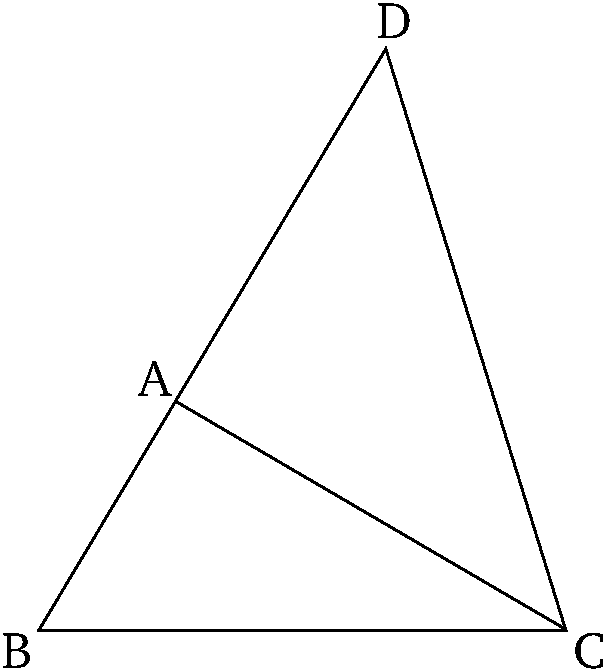
\includegraphics[width=0.8\textwidth]{Book01/fig20e.pdf}}

For let $ABC$ be a triangle. I say that in triangle $ABC$ (the sum of) two
sides taken together in
any (possible way) is greater than the remaining (side). (So), (the sum of) $BA$ and $AC$ (is greater) than $BC$,
(the sum of) $AB$ and $BC$ than $AC$, and (the sum of) $BC$ and $CA$ than $AB$.

For let $BA$ be drawn through to point $D$, and let $AD$ be made equal to $CA$ [Prop.~1.3], and let $DC$ be joined.

Therefore, since $DA$ is equal to $AC$, the angle $ADC$ is also equal to
$ACD$ [Prop.~1.5]. Thus, $BCD$ is greater than $ADC$. And since
 $DCB$ is a triangle having the angle $BCD$ greater than $BDC$, and the
greater angle subtends the greater side [Prop.~1.19], $DB$ is thus
greater than $BC$. But $DA$ is equal to $AC$. Thus, (the sum of) $BA$ and $AC$ is
greater than $BC$. Similarly, we can show that (the sum of) $AB$ and $BC$ is also
greater than $CA$, and (the sum of) $BC$ and $CA$ than $AB$.

Thus, in any triangle, (the sum of) two sides taken together in any (possible way) is greater than the remaining (side). (Which is) the very thing
it was required to show.}
\end{Parallel}

%%%%%%
% Prop 1.21
%%%%%%
\pdfbookmark[1]{Proposition 1.21}{pdf1.21}
\begin{Parallel}{}{} 
\ParallelLText{
\begin{center}
{\large \ggn{21}.}
\end{center}\vspace*{-7pt}

\gr{Ἐὰν τριγώνου ἐπὶ μιᾶς τῶν πλευρῶν ἀπὸ τῶν περάτων δύο
εὐθεῖαι ἐντὸς συσταθῶσιν, αἱ συσταθεῖσαι τῶν λοιπῶν τοῦ
τριγώνου δύο πλευρῶν ἐλάττονες μὲνὸέσονται, μείζονα δὲ
γωνίαν περιέχουσιν.}

\gr{Τριγώνου γὰρ τοῦ ΑΒΓ ἐπὶ μιᾶς τῶν πλευρῶν τῆς ΒΓ ἀπὸ
τῶν περάτων τῶν Β, Γ δύο εὐθεῖαι ἐντὸς συνεστάτωσαν αἱ ΒΔ, ΔΓ;
λέγω, ὅτι αἱ ΒΔ, ΔΓ τῶν λοιπῶν τοῦ τριγώνου δύο πλευρῶν
τῶν ΒΑ, ΑΓ ἐλάσσονες μέν εἰσιν, μείζονα δὲ γωνίαν περιέθουσι
τὴν ὑπὸ ΒΔΓ τῆς ὑπὸ ΒΑΓ.}

% Removed epsf size command
\centerline{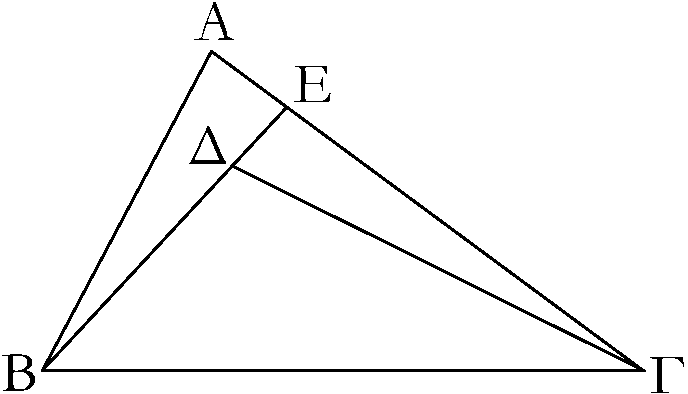
\includegraphics[width=0.8\textwidth]{Book01/fig21g.pdf}}

\gr{Διήθθω γὰρ ἡ ΒΔ ἐπὶ τὸ Ε. καὶ ἐπεὶ παντὸς τριγώνου αἱ δύο
πλευραὶ τῆς λοιπῆς μείζονέξ εἰσιν, τοῦ ΑΒΕ ἄρα τριγώνου αἱ
δύο πλευραὶ αἱ ΑΒ, ΑΕ τῆς ΒΕ μείζονέξ εἰσιν; κοινὴ προσκείσθω
ἡ ΕΓ; αἱ  ἄρα ΒΑ, ΑΓ τῶν ΒΕ, ΕΓ μείζονέξ εἰσιν. πάλιν, ἐπεὶ
τοῦ ΓΕΔ τριγώνου αἱ δύο πλευραὶ αἱ ΓΕ, ΕΔ τῆς ΓΔ μείζονέξ εἰσιν, κοινὴ προσκείσθω ἡ ΔΒ; αἱ ΓΕ, ΕΒ ἄρα τῶν ΓΔ, ΔΒ μείζονέξ εἰσιν. 
ἀλλὰ τῶν ΒΕ, ΕΓ μείζονες ἐδείθθησαν αἱ ΒΑ, ΑΓ; πολλῶ|
 ἄρα αἱ ΒΑ, ΑΓ τῶν ΒΔ, ΔΓ μείζονέξ εἰσιν.}

\gr{Πάλιν, ἐπεὶ παντὸς τριγώνου ἡ ἐκτὸξ γωνία τῆς ἐντὸς
καὶ ἀπεναντίον μείζων ἐστίν, τοῦ ΓΔΕ ἄρα τριγώνου ἡ
ἐκτὸξ γωνία ἡ ὑπὸ ΒΔΓ μείζων ἐστὶ τῆς ὑπὸ ΓΕΔ. διὰ ταὐτὰ
τοίνυν καὶ τοῦ ΑΒΕ τριγώνου ἡ ἐκτὸξ γωνία ἡ ὑπὸ ΓΕΒ μείζων
ἐστὶ τῆς ὑπὸ ΒΑΓ. ἀλλὰ τῆς ὑπὸ ΓΕΒ μείζων ἐδείθθη ἡ
ὑπὸ ΒΔΓ; πολλῶ|  ἄρα ἡ ὑπὸ ΒΔΓ μείζων ἐστὶ τῆς
ὑπὸ ΒΑΓ.}

\gr{Ἐὰν ἄρα τριγώνου ἐπὶ μιᾶς τῶν πλευρῶν ἀπὸ τῶν περάτων δύο
εὐθεῖαι ἐντὸς συσταθῶσιν, αἱ συσταθεῖσαι τῶν λοιπῶν τοῦ
τριγώνου δύο πλευρῶν ἐλάττονες μέν εἰσιν, μείζονα δὲ
γωνίαν περιέθουσιν;  ὅπερ ἔδει δεῖχαι.}}

\ParallelRText{
\begin{center}
{\large Proposition 21}
\end{center}

If two internal straight-lines are constructed on one of the sides
of a triangle, from its ends, 
the constructed (straight-lines) will be less than the two remaining 
sides of the triangle, but will encompass a greater angle.

For let the two internal straight-lines $BD$ and $DC$ be constructed on one of the sides $BC$ of the triangle $ABC$, from its ends $B$ and $C$ (respectively). I say that 
$BD$ and $DC$ are less than the (sum of the) two  remaining sides of the triangle
$BA$ and $AC$, but encompass an angle $BDC$ greater than $BAC$.

% Removed epsf size command
\centerline{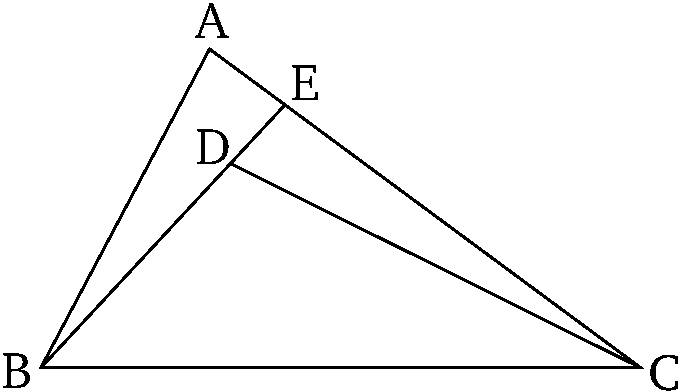
\includegraphics[width=0.8\textwidth]{Book01/fig21e.pdf}}

For let $BD$ be drawn through to $E$. And since in any
triangle (the sum of any) two sides is greater than the remaining (side) [Prop.~1.20],
 in triangle $ABE$ the  (sum of the) two sides $AB$ and $AE$ is thus  greater than
$BE$. Let $EC$ be added to both. Thus, (the sum of) $BA$ and $AC$ is greater
than (the sum of) $BE$ and $EC$.  Again, since in triangle $CED$ the (sum of the) two sides $CE$ and $ED$
is  greater than $CD$, let $DB$ be added to both. Thus, 
(the sum of) $CE$ and $EB$ is greater than  (the sum of) $CD$ and $DB$. But, (the sum of) $BA$ and $AC$ was shown
(to be) greater than (the sum of) $BE$
 and $EC$. Thus, (the sum of) $BA$ and $AC$ is much greater than
(the sum of) $BD$ and $DC$.

Again, since in any  triangle the external angle 
is greater than the internal and opposite (angles) [Prop. 1.16],
 in triangle $CDE$ the external angle $BDC$ is thus greater
than $CED$.  Accordingly, for the same (reason),  the external angle $CEB$ of the
triangle $ABE$ is also greater than $BAC$. But, $BDC$ was shown (to be) 
greater
than $CEB$. Thus, $BDC$ is much greater than $BAC$.

Thus, if two internal straight-lines are constructed on one of the sides
of a triangle, from its ends, 
the constructed (straight-lines) are less than the two remaining 
sides of the triangle, but  encompass a greater angle. (Which is) the
very thing it was required to show.}
\end{Parallel}

%%%%%%
% Prop 1.22
%%%%%%
\pdfbookmark[1]{Proposition 1.22}{pdf1.22}
\begin{Parallel}{}{} 
\ParallelLText{
\begin{center}
{\large \ggn{22}.}
\end{center}\vspace*{-7pt}

\gr{Ἐκ τριῶν εὐθειῶν, αὁί εἰσιν ἴσαι τρισὶ ταῖς δοθείσαις [εὐθείαις], τρίγωνον συστήσασθαι; δεῖ δὲ τὰξ δύο τῆς λοιπῆς μείζονας εὸῖναι
πάντῃ μεταλαμβανομένας [διὰ τὸ καὶ παντὸς τριγώνου τὰξ δύο πλευρὰξ τῆς λοιπῆς μείζονας εὸῖναι πάντῃ μεταλαμβανομένας].}\\~\\

% Removed epsf size command
\centerline{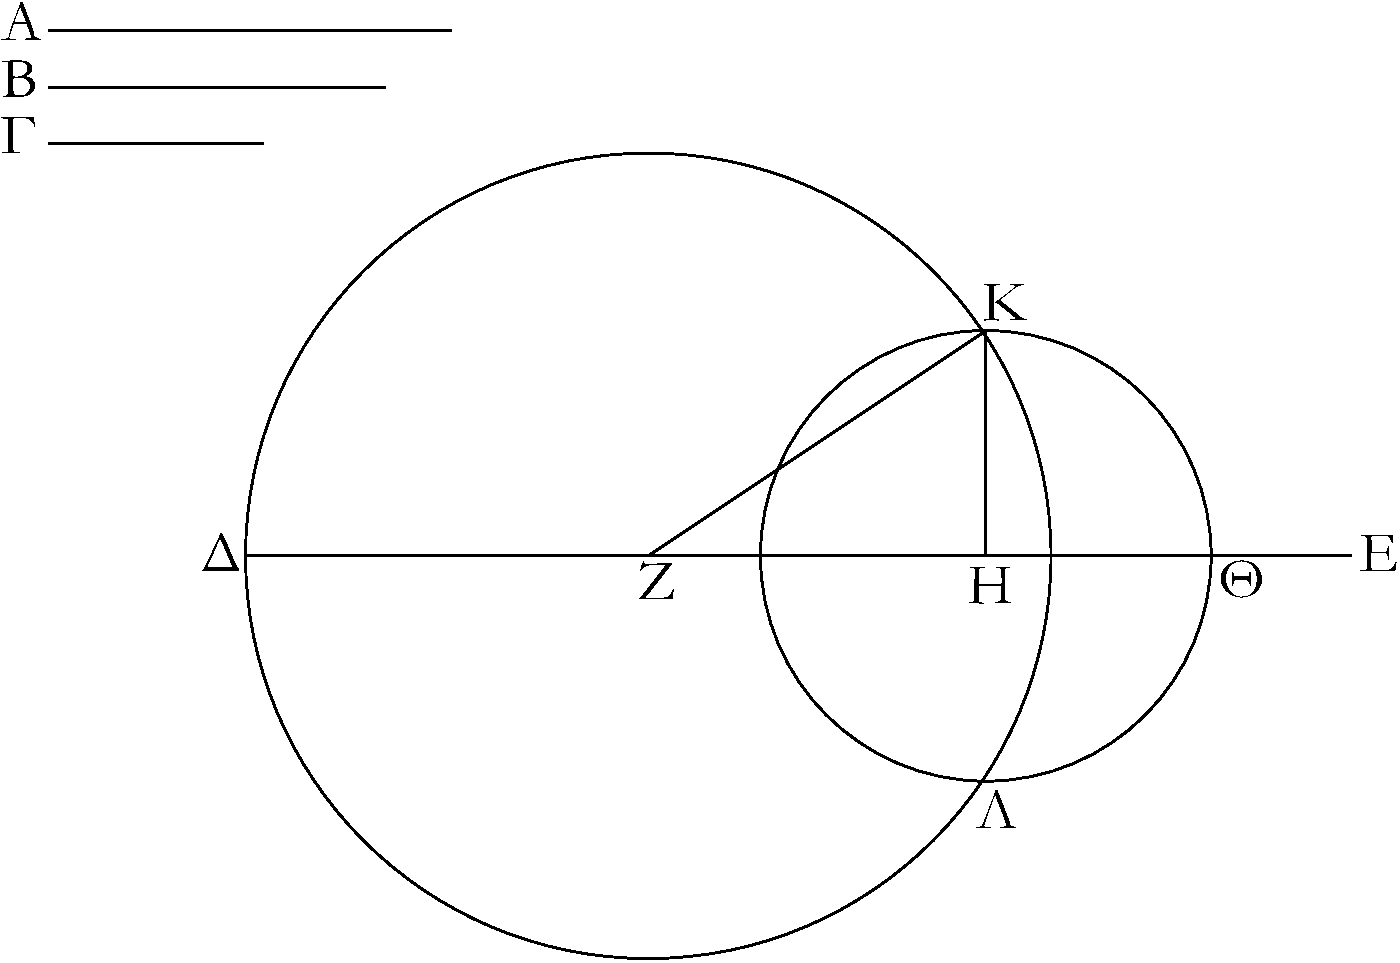
\includegraphics[width=0.8\textwidth]{Book01/fig22g.pdf}}

\gr{Ἔστωσαν αἱ δοθεῖσαι τρεῖς εὐθεῖαι αἱ Α, Β, Γ, ὁῶν αἱ δύο τῆς
λοιπῆς μείζονεςὸέστωσαν πάντῃ μεταλαμβανόμεναι, αἱ μὲν Α, Β
τῆς Γ, αἱ δὲ Α, Γ τῆς Β, καὶ ὸέτι αἱ Β, Γ τῆς Α; δεῖ δὴ ἐκ
τῶνὸίσων ταῖς Α, Β, Γ τρίγωνον συστήσασθαι.}

\gr{Ἐκκείσθω τις εὐθεῖα ἡ ΔΕ πεπερασμένη μὲν κατὰ τὸ Δὸάπειρος
δὲ κατὰ τὸ Ε, καὶ κείσθω τῇ μὲν Αὸίση ἡ ΔΖ, τῇ δὲ Βὸίση ἡ ΖΗ, τῇ δὲ Γὸίση ἡ ΗΘ; καὶ κέντρῳ μὲν τῷ Ζ, διαστήματι δὲ τῷ
ΖΔ κύκλος γεγράφθω ὁ ΔΚΛ; πάλιν κέντρῳ μὲν τῷ Η, διαστήματι δὲ τῷ ΗΘ κύκλος γεγράφθω ὁ ΚΛΘ, καὶ ἐπεζεύθθωσαν αἱ ΚΖ, ΚΗ; λέγω,
ὅτι ἐκ τριῶν εὐθειῶν τῶνὸίσων ταῖς Α, Β, Γ τρίγωνον συνέσταται τὸ ΚΖΗ.}

\gr{Ἐπεὶ γὰρ τὸ Ζ σημεῖον κέντρον ἐστὶ τοῦ ΔΚΛ κύκλου, ὸίση ἐστὶν ἡ ΖΔ τῇ ΖΚ; ἀλλὰ ἡ ΖΔ τῇ Α ἐστινὸίση. καὶ ἡ ΚΖ ἄρα τῇ 
Α ἐστινὸίση. πάλιν, ἐπεὶ τὸ Η σημεῖον κέντρον ἐστὶ τοῦ ΛΚΘ
κύκλου, ὸίση ἐστὶν ἡ ΗΘ τῇ ΗΚ; ἀλλὰ ἡ ΗΘ τῇ Γ ἐστινὸίση;
καὶ ἡ ΚΗ ἄρα τῇ Γ ἐστινὸίση. ἐστὶ δὲ καὶ ἡ ΖΗ τῇ Βὸίση;
αἱ τρεῖς ἄρα εὐθεῖαι αἱ ΚΖ, ΖΗ, ΗΚ τρισὶ ταῖς Α, Β, Γ ἴσαι εἰσίν.}

\gr{Ἐκ τριῶν ἄρα εὐθειῶν τῶν ΚΖ, ΖΗ, ΗΚ, αὁί εἰσιν ἴσαι τρισὶ ταῖς δοθείσαις εὐθείαις ταῖς Α, Β, Γ, τρίγωνον συνέσταται τὸ ΚΖΗ; ὅπερ ἔδει ποιῆσαι.}}

\ParallelRText{
\begin{center}
{\large Proposition 22}
\end{center}

To construct a triangle from three straight-lines which are equal to three given [straight-lines]. It is necessary for (the sum of) two (of the straight-lines) taken together in any (possible way) to be greater than the remaining (one), [on account of the (fact that)
 in any triangle (the sum of) two sides taken together in any (possible way) is greater than the remaining (one) [Prop.~1.20]\,].

% Removed epsf size command
\centerline{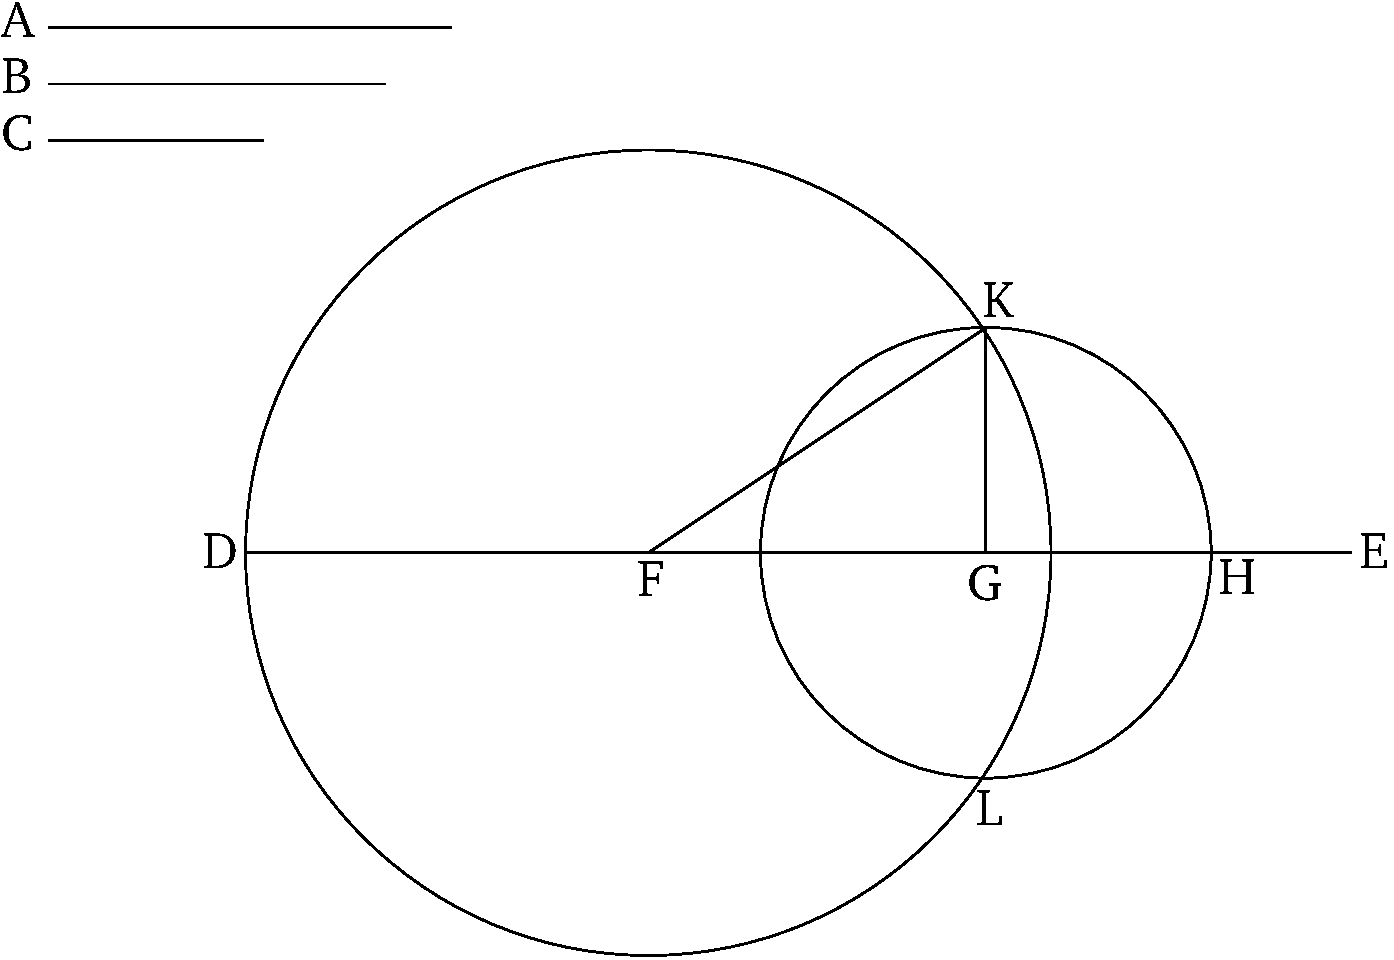
\includegraphics[width=0.8\textwidth]{Book01/fig22e.pdf}}

Let $A$, $B$, and $C$ be the three given straight-lines, of which let (the sum of) two taken together in any (possible way)
be greater than the remaining (one). (Thus), (the sum of) $A$ and $B$ (is greater) than $C$, (the sum of) $A$ and $C$ than $B$,
and also (the sum of) $B$ and $C$ than $A$. So it is required to construct a triangle
from (straight-lines) equal to $A$, $B$, and $C$.

Let some straight-line $DE$ be set out, terminated at $D$, and infinite in the
direction of $E$.  And let $DF$ made equal to $A$, and $FG$
equal to $B$, and $GH$ equal to $C$ [Prop.~1.3]. And let the
circle $DKL$ be drawn with center $F$ and radius $FD$. Again,
let the circle $KLH$ be drawn with center $G$ and radius $GH$. And
let $KF$ and $KG$ be joined. I say that the triangle $KFG$ has been
constructed from three straight-lines equal to $A$, $B$, and $C$.

For since point $F$ is the center of the circle $DKL$, $FD$ is equal to $FK$.
But, $FD$ is equal to $A$. Thus, $KF$ is also equal to $A$. Again, since point
$G$ is the center of the circle $LKH$, $GH$ is equal to $GK$. But, $GH$ is equal
to $C$. Thus, $KG$ is also equal to $C$. And $FG$ is also equal to $B$. Thus,
the three straight-lines $KF$, $FG$, and $GK$ are equal to $A$, $B$, and $C$ (respectively).

Thus, the triangle $KFG$ has been constructed from the three straight-lines
$KF$, $FG$, and $GK$, which are equal to the three given straight-lines
$A$, $B$, and $C$ (respectively). (Which is) the very thing it was required
to do.}
\end{Parallel}

%%%%%%
% Prop 1.23
%%%%%%
\pdfbookmark[1]{Proposition 1.23}{pdf1.23}
\begin{Parallel}{}{} 
\ParallelLText{
\begin{center}
{\large \ggn{23}.}
\end{center}\vspace*{-7pt}

\gr{Πρὸξ τῇ δοθείσῃ εὐθείᾳ καὶ τῷ πρὸς αὐτῇ σημείῳ τῇ δοθείσῃ
γωνίᾳ εὐθυγράμμῳ  ἴσην γωνίαν εὐθύγραμμον συστήσασθαι.}

\gr{Ἔστω ἡ μὲν δοθεῖσα εὐθεῖα ἡ ΑΒ, τὸ δὲ πρὸς αὐτῇ σημεῖον τὸ
Α, ἡ δὲ δοθεῖσα γωνία εὐθύγραμμος ἡ ὑπὸ ΔΓΕ; δεῖ δὴ πρὸς
τῇ δοθείσῃ εὐθείᾳ τῇ ΑΒ καὶ τῷ πρὸς αὐτῇ σημείῳ τῷ Α
τῇ δοθείσῃ γωνίᾳ εὐθυγράμμῳ τῇ ὑπὸ ΔΓΕ ἴσην γωνίαν εὐθύγραμμον συστήσασθαι.}

% Removed epsf size command
\centerline{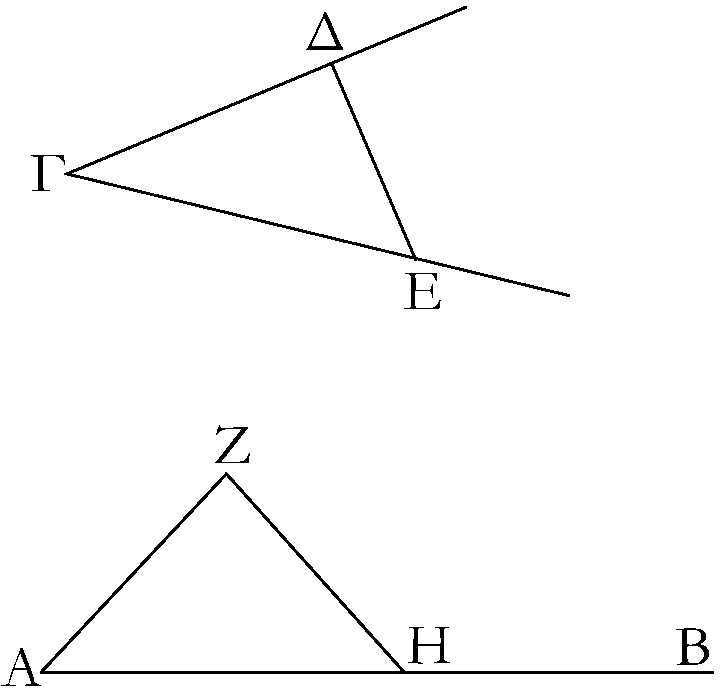
\includegraphics[width=0.8\textwidth]{Book01/fig23g.pdf}}

\gr{Εἰλήφθω ἐφ' ἑκατέρας τῶν ΓΔ, ΓΕ τυθόντα σημεῖα τὰ Δ, Ε, καὶ
ἐπεζεύθθω ἡ ΔΕ; καὶ ἐκ τριῶν εὐθειῶν, αὁί εἰσιν ἴσαι τρισὶ ταῖς
ΓΔ, ΔΕ, ΓΕ, τρίγωνον συνεστάτω τὸ ΑΖΗ, ὁώστε ἴσην εὸῖναι τὴν
μὲν ΓΔ τῇ ΑΖ, τὴν δὲ ΓΕ τῇ ΑΗ, καὶ ὸέτι τὴν ΔΕ τῇ ΖΗ.}

\gr{Ἐπεὶ οὸῦν δύο αἱ ΔΓ, ΓΕ δύο ταῖς ΖΑ, ΑΗ ἴσαι εἰσὶν ἑκατέρα ἑκατέρᾳ, καὶ βάσις ἡ ΔΕ βάσει τῇ ΖΗὸίση, γωνία ἄρα ἡ ὑπὸ
ΔΓΕ γωνίᾳ τῇ ὑπὸ ΖΑΗ ἐστινὸίση.}

\gr{Πρὸξ ἄρα τῇ δοθείσῃ εὐθείᾳ τῇ ΑΒ καὶ τῷ πρὸς αὐτῇ σημείῳ
τῷ Α τῇ δοθείσῃ γωνίᾳ εὐθυγράμμῳ τῇ ὑπὸ ΔΓΕὸίση γωνία εὐθύγραμμος συνέσταται ἡ ὑπὸ ΖΑΗ; ὅπερ ἔδει ποιῆσαι.}}

\ParallelRText{
\begin{center}
{\large Proposition 23}
\end{center}

To construct a rectilinear angle equal to a given rectilinear angle at a (given)
point on a given straight-line.

Let $AB$ be the given straight-line,  $A$ the (given) point on it, and 
$DCE$ the given rectilinear angle. So it is required to construct a rectilinear
angle equal to the given rectilinear angle $DCE$ at the (given) point
$A$ on the given straight-line
$AB$.\\~\\

% Removed epsf size command
\centerline{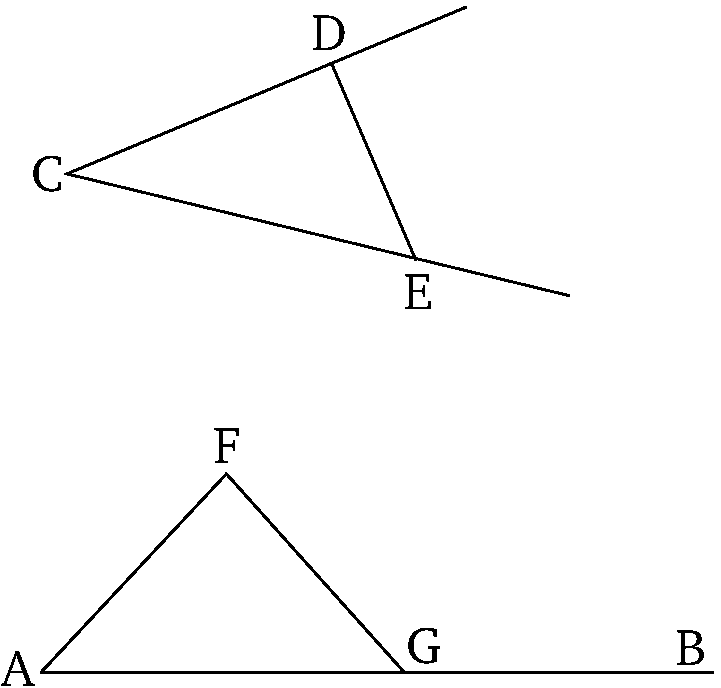
\includegraphics[width=0.8\textwidth]{Book01/fig23e.pdf}}

Let the points $D$ and $E$ be taken at random on each
of the (straight-lines) $CD$ and $CE$ (respectively), and let $DE$ be joined.
And let the triangle $AFG$ be constructed from three straight-lines
which are equal to $CD$, $DE$, and $CE$, such that $CD$ is equal to $AF$,
$CE$ to $AG$, and further $DE$ to $FG$ [Prop.~1.22].

Therefore, since the two (straight-lines) $DC$, $CE$ are equal to the
two (straight-lines) $FA$, $AG$, respectively, and the base $DE$ is equal to
the base $FG$, the angle $DCE$ is thus equal to the angle $FAG$ [Prop.~1.8].

Thus, the rectilinear angle $FAG$,  equal to the  given
rectilinear angle $DCE$, has been constructed at the (given) point $A$ on the given straight-line $AB$.
(Which is) the very thing it was required to do.}
\end{Parallel}

%%%%%%
% Prop 1.24
%%%%%%
\pdfbookmark[1]{Proposition 1.24}{pdf1.24}
\begin{Parallel}{}{} 
\ParallelLText{
\begin{center}
{\large\ggn{24}.}
\end{center}\vspace*{-7pt}

\gr{Ἐὰν δύο τρίγωνα τὰξ δύο πλευρὰξ [ταῖς] δύο πλευραῖξ ἴσαςὸέθῃ ἑκατέραν
ἑκατέρᾳ, τὴν δὲ γωνίαν τῆς γωνίας μείζοναὸέθῃ τὴν ὑπὸ τῶνὸίσων εὐθειῶν περιεθομένην, καὶ τὴν βάσιν τῆς βάσεως μείζονα ὁέχει.}

\gr{Ἔστω δύο τρίγωνα τὰ ΑΒΓ, ΔΕΖ τὰξ δύο πλευρὰξ τὰξ ΑΒ, ΑΓ ταῖς δύο πλευραῖξ ταῖς ΔΕ, ΔΖ ἴσας ἔχοντα ἑκατέραν ἑκατέρᾳ, τὴν μὲν ΑΒ τῇ ΔΕ τὴν δὲ ΑΓ τῇ ΔΖ, ἡ δὲ πρὸς τῷ Α γωνία τῆς πρὸς τῷ Δ γωνίας μείζωνὸέστω; λέγω, ὅτι καὶ βάσις ἡ ΒΓ βάσεως τῆς ΕΖ μείζων ἐστίν.}

\gr{Ἐπεὶ γὰρ μείζων ἡ ὑπὸ ΒΑΓ γωνία τῆς ὑπὸ ΕΔΖ γωνίας, συνεστάτω πρὸς τῇ ΔΕ εὐθείᾳ καὶ τῷ πρὸς αὐτῇ σημείῳ τῷ Δ τῇ ὑπὸ ΒΑΓ γωνίᾳ ὸίση ἡ ὑπὸ ΕΔΗ, καὶ κείσθω ὁποτέρᾳ τῶν ΑΓ, ΔΖὸίση ἡ ΔΗ, καὶ ἐπεζεύθθωσαν αἱ ΕΗ, ΖΗ.}\\

% Removed epsf size command
\centerline{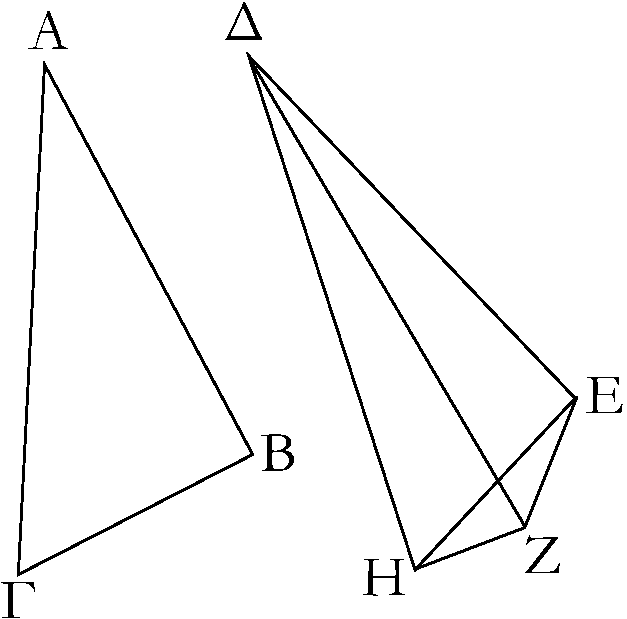
\includegraphics[width=0.8\textwidth]{Book01/fig24g.pdf}}

\gr{Ἐπεὶ οὸῦνὸίση ἐστὶν ἡ μὲν ΑΒ τῇ ΔΕ, ἡ δὲ ΑΓ τῇ ΔΗ, δύο
δὴ αἱ ΒΑ, ΑΓ δυσὶ ταῖς ΕΔ, ΔΗ ἴσαι εἰσὶν ἑκατέρα ἑκατέρᾳ;
καὶ γωνία ἡ ὑπὸ ΒΑΓ γωνίᾳ τῇ ὑπὸ ΕΔΗὸίση; βάσις ἄρα ἡ ΒΓ βάσει τῇ ΕΗ ἐστινὸίση.  πάλιν, ἐπεὶ ὸίση ἐστὶν ἡ ΔΖ τῇ ΔΗ, ὸίση ἐστὶ καὶ ἡ
ὑπὸ ΔΗΖ γωνία τῇ ὑπὸ ΔΖΗ; μείζων ἄρα ἡ ὑπὸ ΔΖΗ τῆς ὑπὸ ΕΗΖ; πολλῶ|  ἄρα μείζων ἐστὶν ἡ ὑπὸ ΕΖΗ τῆς ὑπὸ ΕΗΖ.
καὶ ἐπεὶ τρίγωνόν ἐστι τὸ ΕΖΗ μείζονα ἔχον τὴν ὑπὸ ΕΖΗ γωνίαν τῆς ὑπὸ ΕΗΖ, ὑπὸ δὲ τὴν μείζονα γωνίαν ἡ μείζων πλευρὰ ὑποτείνει, μείζων ἄρα καὶ πλευρὰ ἡ ΕΗ τῆς ΕΖ. ὸίση δὲ ἡ ΕΗ τῇ
ΒΓ; μείζων ἄρα καὶ ἡ ΒΓ τῆς ΕΖ.}

\gr{Ἐὰν ἄρα δύο τρίγωνα τὰξ δύο πλευρὰξ δυσὶ πλευραῖξ ἴσαςὸέθῃ ἑκατέραν
ἑκατέρᾳ, τὴν δὲ γωνίαν τῆς γωνίας μείζοναὸέθῃ τὴν ὑπὸ τῶνὸίσων εὐθειῶν περιεθομένην, καὶ τὴν βάσιν τῆς βάσεως μείζονα ὁέχει; ὅπερ ἔδει δεῖχαι.}}

\ParallelRText{
\begin{center}
{\large Proposition 24}
\end{center}

If two triangles have two sides equal to two sides, respectively,
but (one) has the angle encompassed by the equal straight-lines greater than the (corresponding)
angle (in the other),  (then the former triangle) will also have a base greater than the base (of the latter).

Let  $ABC$ and $DEF$ be two triangles having the two sides $AB$ and $AC$
equal to the two sides $DE$ and $DF$, respectively. (That is), $AB$ (equal) to $DE$, and
$AC$ to $DF$.  Let them also have the angle at $A$ greater than the angle at $D$.
I say that the base $BC$ is also greater than the base $EF$.

For since angle $BAC$ is greater than angle $EDF$, let (angle) $EDG$, equal to
angle $BAC$,  be constructed at  the point $D$ on the straight-line $DE$ [Prop.~1.23]. And let $DG$ be made equal to either of $AC$ or $DF$ [Prop.~1.3], and let $EG$ and $FG$ be joined.

% Removed epsf size command
\centerline{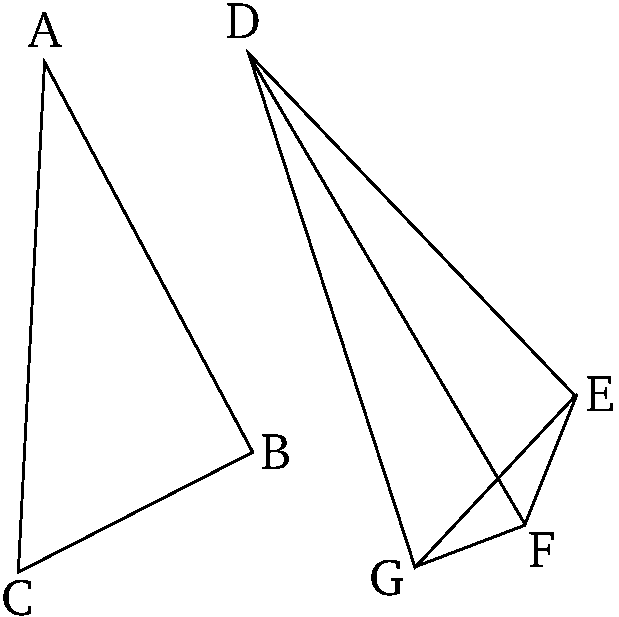
\includegraphics[width=0.8\textwidth]{Book01/fig24e.pdf}}

Therefore, since $AB$ is equal to $DE$ and $AC$ to $DG$, the two (straight-lines)
$BA$, $AC$ are equal to the two (straight-lines) $ED$, $DG$, respectively.
Also the angle $BAC$ is equal to the angle $EDG$. Thus, the base $BC$ is equal
to the base $EG$ [Prop.~1.4]. Again, since $DF$ is equal to $DG$, angle $DGF$
is also equal to angle $DFG$ [Prop.~1.5]. Thus, $DFG$ (is) greater than $EGF$.
Thus, $EFG$ is much greater than $EGF$. And since triangle $EFG$ has angle $EFG$
greater than $EGF$, and the greater angle is subtended by the greater side [Prop.~1.19], side $EG$ (is) thus also greater than $EF$. But $EG$ (is) equal to
$BC$. Thus, $BC$ (is) also greater than $EF$.

Thus, if two triangles have two sides equal to two sides, respectively,
but (one) has the angle encompassed by the equal straight-lines greater than the 
(corresponding) angle (in the other), (then the former triangle) will also have a base greater than the base (of the latter).
(Which is) the very thing it was required to show.}
\end{Parallel}

%%%%%%
% Prop 1.25
%%%%%%
\pdfbookmark[1]{Proposition 1.25}{pdf1.25}
\begin{Parallel}{}{} 
\ParallelLText{
\begin{center}
{\large \ggn{25}.}
\end{center}\vspace*{-7pt}

\gr{Ἐὰν δύο τρίγωνα τὰξ δύο πλευρὰξ δυσὶ πλευραῖξ ἴσαςὸέθῃ ἑκατέραν ἑκατέρᾳ, τὴν δὲ βάσιν τῆς βάσεως μείζοναὸέθῃ, καὶ τὴν γωνίαν τῆς γωνίας μείζονα ὁέχει τὴν ὑπὸ τῶνὸίσων εὐθειῶν περιεθομένην.}

\gr{Ἔστω δύο τρίγωνα τὰ ΑΒΓ, ΔΕΖ τὰξ δύο πλευρὰξ τὰξ ΑΒ, ΑΓ ταῖς δύο πλευραῖξ ταῖς ΔΕ, ΔΖ ἴσας ἔχοντα ἑκατέραν ἑκατέρᾳ, τὴν μὲν ΑΒ
τῇ ΔΕ, τὴν δὲ ΑΓ τῇ ΔΖ; βάσις δὲ ἡ ΒΓ βάσεως τῆς ΕΖ μείζωνὸέστω; λέγω, ὅτι καὶ γωνία ἡ ὑπὸ ΒΑΓ γωνίας τῆς ὑπὸ ΕΔΖ μείζων ἐστίν.}

\gr{Εἰ γὰρ μή,  ἢτοιὸίση ἐστὶν αὐτῇ ὸὴ ἐλάσσων; ὸίση μὲν οὸῦν οὐκὸέστιν ἡ ὑπὸ ΒΑΓ τῇ ὑπὸ ΕΔΖ; ὸίση γὰρὸὰνὸῆν καὶ βάσις ἡ ΒΓ βάσει τῇ ΕΖ; οὐκὸέστι δέ. οὐκ ἄραὸίση ἐστὶ γωνία ἡ ὑπὸ ΒΑΓ τῇ ὑπὸ ΕΔΖ; οὐδὲ μὴν ἐλάσσων ἐστὶν ἡ ὑπὸ ΒΑΓ τῆς ὑπὸ ΕΔΖ; ἐλάσσων γὰρὸὰνὸῆν καὶ βάσις ἡ ΒΓ βάσεως τῆς ΕΖ; οὐκὸέστι δέ; οὐκ ἄρα ἐλάσσων ἐστὶν ἡ ὑπὸ ΒΑΓ γωνία τῆς ὑπὸ ΕΔΖ. ἐδείθθη δέ, ὅτι οὐδὲ ὸίση; μείζων ἄρα ἐστὶν ἡ ὑπὸ ΒΑΓ τῆς ὑπὸ ΕΔΖ.}\\

% Removed epsf size command
\centerline{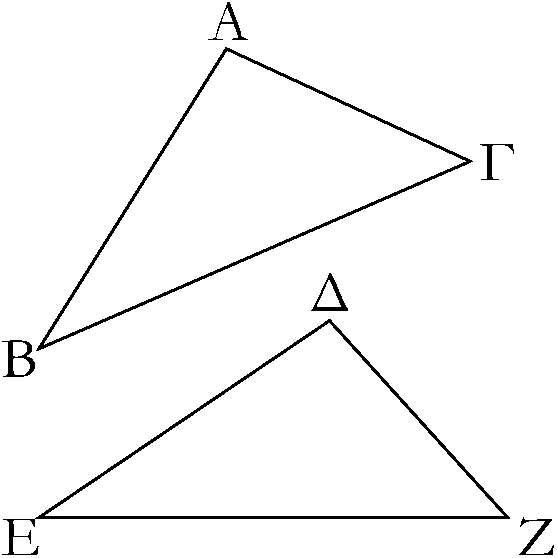
\includegraphics[width=0.8\textwidth]{Book01/fig25g.pdf}}

\gr{Ἐὰν ἄρα δύο τρίγωνα τὰξ δύο πλευρὰξ δυσὶ πλευραῖξ ἴσαςὸέθῃ ἑκατέραν ἑκάτερᾳ, τὴν δὲ βασίν τῆς βάσεως μείζοναὸέθῃ, καὶ τὴν γωνίαν τῆς γωνίας μείζονα ὁέχει τὴν ὑπὸ τῶνὸίσων εὐθειῶν περιεθομένην; ὅπερ ἔδει δεῖχαι.}}

\ParallelRText{
\begin{center}
{\large Proposition 25}
\end{center}

If two triangles have two sides equal to two sides, respectively,
but (one) has a base greater than the base (of the other), (then the former triangle) will also have the angle encompassed by the equal straight-lines greater than the (corresponding) angle (in the latter).

Let $ABC$ and $DEF$ be  two triangles having the two sides $AB$ and $AC$
equal to the two sides $DE$ and $DF$, respectively (That is), $AB$ (equal) to $DE$, and $AC$ to $DF$. And let the base $BC$ be greater than the base $EF$. I say that angle
$BAC$ is also greater than $EDF$.

For if not, ($BAC$) is certainly either equal to, or less than, ($EDF$). In fact, $BAC$ is not equal to
$EDF$. For then the base $BC$ would also be equal to the base $EF$ [Prop.~1.4]. But it is not.
Thus, angle $BAC$ is not equal to $EDF$. Neither, indeed, is $BAC$ less
than $EDF$. For then the base $BC$ would also be less than the base $EF$ [Prop.~1.24].
But it is not. Thus, angle $BAC$ is not less than $EDF$. But it was  shown
that ($BAC$ is) not equal (to $EDF$) either. Thus, $BAC$ is greater than $EDF$.

% Removed epsf size command
\centerline{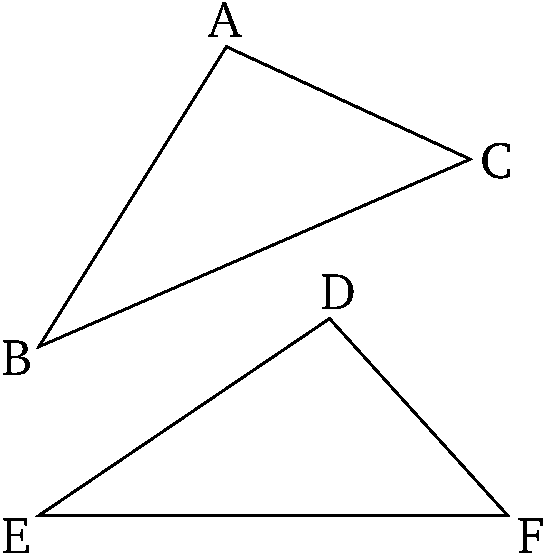
\includegraphics[width=0.8\textwidth]{Book01/fig25e.pdf}}

Thus, if two triangles have two sides equal to two sides, respectively,
but (one) has a base greater than the base (of the other), (then the former triangle) will also have the angle encompassed by the equal straight-lines greater than the (corresponding) angle (in the latter). (Which is) the
very thing it was required to show.}
\end{Parallel}

%%%%%%
% Prop 1.26
%%%%%%
\pdfbookmark[1]{Proposition 1.26}{pdf1.26}
\begin{Parallel}{}{} 
\ParallelLText{
\begin{center}
{\large \ggn{26}.}
\end{center}\vspace*{-7pt}

\gr{Ἐὰν δύο τρίγωνα τὰξ δύο γωνίας δυσὶ γωνίαις ἴσαςὸέθῃ ἑκατέραν
ἑκατέρᾳ καὶ μίαν πλευρὰν μιᾶ| πλευρᾶ|  ἴσην ἢτοι τὴν πρὸς ταῖς ἴσαις γωνίαιςὸὴ τὴν ὑποτείνουσαν ὑπὸ μίαν τῶνὸίσων γωνιῶν, καὶ τὰξ λοιπὰξ πλευρὰξ ταῖς λοιπαῖξ πλευραῖξ ἴσας ὁέχει [ἑκατέραν
ἑκατέρᾳ] καὶ τὴν λοιπὴν γωνίαν τῇ λοιπῆ| γωνίᾳ.}

\gr{Ἔστω δύο τρίγωνα τὰ ΑΒΓ, ΔΕΖ τὰξ δύο γωνίας τὰξ ὑπὸ ΑΒΓ, ΒΓΑ δυσὶ ταῖς ὑπὸ ΔΕΖ, ΕΖΔ ἴσας ἔχοντα ἑκατέραν ἑκατέρᾳ, τὴν μὲν ὑπὸ ΑΒΓ τῇ ὑπὸ ΔΕΖ, τὴν δὲ ὑπὸ ΒΓΑ τῇ ὑπὸ ΕΖΔ; ἐθέτω δὲ καὶ μίαν πλευρὰν μιᾶ| πλευρᾶ|  ἴσην, πρότερον τὴν πρὸς ταῖς ἴσαις γωνίαις τὴν ΒΓ τῇ ΕΖ; λέγω, ὅτι καὶ τὰξ λοιπὰξ πλευρὰξ ταῖς λοιπαῖξ πλευραῖξ ἴσας ὁέχει ἑκατέραν ἑκατέρᾳ, τὴν μὲν ΑΒ τῇ ΔΕ τὴν δὲ ΑΓ τῇ ΔΖ, καὶ τὴν λοιπὴν γωνίαν τῇ λοιπῆ| γωνίᾳ, τὴν ὑπὸ ΒΑΓ τῇ ὑπὸ ΕΔΖ.}

\gr{Εἰ γὰρὸάνισόξ ἐστιν ἡ ΑΒ τῇ ΔΕ, μία αὐτῶν μείζων ἐστίν.
ὸέστω μείζων ἡ ΑΒ, καὶ κείσθω τῇ ΔΕὸίση ἡ ΒΗ, καὶ ἐπεζεύθθω ἡ ΗΓ.}

\gr{Ἐπεὶ οὸῦνὸίση ἐστὶν ἡ μὲν ΒΗ τῇ ΔΕ, ἡ δὲ ΒΓ τῇ ΕΖ, δύο δὴ αἱ ΒΗ, ΒΓ δυσὶ ταῖς ΔΕ, ΕΖ ἴσαι εἰσὶν ἑκατέρα ἑκατέρᾳ; καὶ γωνία ἡ ὑπὸ ΗΒΓ γωνίᾳ τῇ ὑπὸ ΔΕΖὸίση ἐστίν; βάσις ἄρα ἡ ΗΓ βάσει τῇ ΔΖὸίση ἐστίν, καὶ τὸ ΗΒΓ τρίγωνον τῷ ΔΕΖ τριγώνῳ  ἴσον ἐστίν, καὶ αἱ λοιπαὶ γωνίαι ταῖς λοιπαῖξ γωνίαις ἴσαιὸέσονται, ὑφὸ ὁὰξ αἱ  ἴσαι πλευραὶ ὑποτείνουσιν; ὸίση ἄρα ἡ ὑπὸ ΗΓΒ γωνία τῇ ὑπὸ ΔΖΕ. ἀλλὰ ἡ ὑπὸ ΔΖΕ τῇ ὑπὸ ΒΓΑ ὑπόκειταιὸίση;
καὶ ἡ ὑπὸ ΒΓΗ ἄρα τῇ ὑπὸ ΒΓΑὸίση ἐστίν, ἡ ἐλάσσων
τῇ μείζονι; ὅπερ ἀδύνατον. οὐκ ἄραὸάνισόξ ἐστιν ἡ ΑΒ τῇ ΔΕ.
ὸίση ἄρα. ὸέστι δὲ καὶ ἡ ΒΓ τῇ ΕΖὸίση; δύο δὴ αἱ ΑΒ, ΒΓ δυσὶ ταῖς ΔΕ, ΕΖ ἴσαι εἰσὶν ἑκατέρα ἑκατέρᾳ; καὶ γωνία ἡ ὑπὸ ΑΒΓ
γωνίᾳ τῇ ὑπὸ ΔΕΖ ἐστινὸίση; βάσις ἄρα ἡ ΑΓ βάσει τῇ ΔΖὸίση ἐστίν, καὶ λοιπὴ γωνία ἡ ὑπὸ ΒΑΓ τῇ λοιπῆ| γωνίᾳ τῇ ὑπὸ ΕΔΖὸίση ἐστίν.}\\~\\

% Removed epsf size command
\centerline{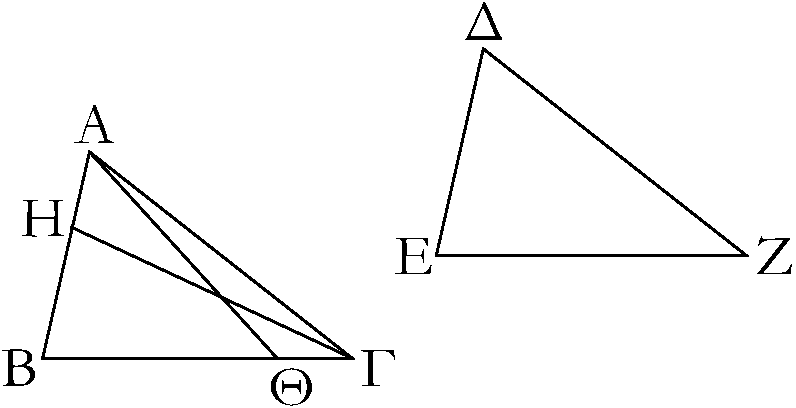
\includegraphics[width=0.8\textwidth]{Book01/fig26g.pdf}}

\gr{Ἀλλὰ δὴ πάλινὸέστωσαν αἱ ὑπὸ τὰξ ἴσας γωνίας πλευραὶ ὑποτείνουσαι ἴσαι, ὡξ ἡ ΑΒ τῇ ΔΕ; λέγω πάλιν, ὅτι καὶ αἱ λοιπαὶ πλευραὶ ταῖς λοιπαῖξ πλευραῖξ ἴσαιὸέσονται, ἡ μὲν ΑΓ τῇ ΔΖ, ἡ δὲ ΒΓ τῇ ΕΖ καὶ ὸέτι ἡ λοιπὴ γωνία ἡ ὑπὸ ΒΑΓ τῇ λοιπῆ| γωνίᾳ τῇ ὑπὸ ΕΔΖὸίση ἐστίν.}

\gr{Εἰ γὰρὸάνισόξ ἐστιν ἡ ΒΓ τῇ ΕΖ, μία αὐτῶν μείζων ἐστίν. ὸέστω μείζων, εἰ δυνατόν, ἡ ΒΓ, καὶ κείσθω τῇ ΕΖὸίση ἡ ΒΘ, καὶ ἐπεζεύθθω ἡ ΑΘ. καὶ ἐπὲιὸίση ἐστὶν ἡ μὲν ΒΘ τῇ ΕΖ ἡ δὲ ΑΒ τῇ ΔΕ, δύο δὴ αἱ ΑΒ, ΒΘ δυσὶ ταῖς ΔΕ, ΕΖ ἴσαι εἰσὶν ἑκατέρα ἑκαρέρᾳ; καὶ γωνίας ἴσας περιέθουσιν; βάσις ἄρα ἡ ΑΘ βάσει τῇ ΔΖὸίση ἐστίν, καὶ τὸ ΑΒΘ τρίγωνον τῷ ΔΕΖ τριγώνῳ  ἴσον ἐστίν, καὶ αἱ λοιπαὶ γωνίαι ταῖς λοιπαῖξ γωνίαις ἴσαιὸέσονται, ὑφὸ ὁὰξ αἱ  ἴσας πλευραὶ ὑποτείνουσιν;
 ὸίση ἄρα ἐστὶν ἡ ὑπὸ ΒΘΑ γωνία τῇ ὑπὸ ΕΖΔ.
ἀλλὰ ἡ ὑπὸ ΕΖΔ τῇ ὑπὸ ΒΓΑ ἐστινὸίση; τριγώνου δὴ τοῦ ΑΘΓ ἡ ἐκτὸξ γωνία ἡ ὑπὸ ΒΘΑὸίση ἐστὶ τῇ ἐντὸς καὶ ἀπεναντίον
τῇ ὑπὸ ΒΓΑ; ὅπερ ἀδύνατον. οὐκ ἄραὸάνισόξ ἐστιν ἡ ΒΓ τῇ ΕΖ; ὸίση ἄρα. ἐστὶ δὲ καὶ ἡ ΑΒ τῇ ΔΕὸίση. δύο δὴ αἱ ΑΒ, ΒΓ δύο ταῖς ΔΕ, ΕΖ ἴσαι εἰσὶν ἑκατέρα ἑκατέρᾳ; καὶ γωνίας ἴσας περιέθουσι; βάσις ἄρα ἡ ΑΓ βάσει τῇ ΔΖὸίση ἐστίν, καὶ τὸ ΑΒΓ τρίγωνον τῷ ΔΕΖ τριγώνῳ  ἴσον καὶ λοιπὴ γωνία ἡ ὑπὸ ΒΑΓ τῇ λοιπὴ| γωνίᾳ τῇ ὑπὸ ΕΔΖὸίση.}

\gr{Ἐὰν ἄρα δύο τρίγωνα τὰξ δύο γωνίας δυσὶ γωνίαις ἴσαςὸέθῃ ἑκατέραν
ἑκατέρᾳ καὶ μίαν πλευρὰν μιᾶ| πλευρᾶ|  ἴσην ἢτοι τὴν πρὸς ταῖς ἴσαις γωνίαις, ὸὴ τὴν ὑποτείνουσαν ὑπὸ μίαν τῶνὸίσων γωνιῶν, καὶ τὰξ λοιπὰξ πλευρὰξ ταῖς λοιπαῖξ πλευραῖξ ἴσας ὁέχει 
καὶ τὴν λοιπὴν γωνίαν τῇ λοιπῆ| γωνίᾳ; ὅπερ ἔδει δεῖχαι.}}

\ParallelRText{
\begin{center}
{\large Proposition 26}
\end{center}

If  two triangles have two angles equal to two angles, respectively, 
and one side equal to one side---in fact, either that by the equal angles, or that
subtending one of the equal angles---(then the triangles) will also have the remaining
sides equal to the [corresponding] remaining sides, and the
remaining angle (equal) to the remaining angle.

Let $ABC$ and $DEF$ be two triangles having the two angles $ABC$ and
$BCA$ equal to the two (angles) $DEF$ and $EFD$, respectively.
(That is) $ABC$ (equal) to $DEF$, and $BCA$ to $EFD$. And let them also have
one side equal to one side. First of all, the (side) by the equal angles. (That is)
$BC$ (equal) to $EF$. I say that they will have the  remaining sides equal to the
corresponding remaining sides. (That is) $AB$ (equal) to $DE$, and $AC$ to
$DF$. And (they will have) the remaining angle (equal) to the remaining angle.
(That is) $BAC$ (equal) to $EDF$.

For if $AB$ is unequal to $DE$ (then) one of them is greater. Let $AB$ be greater,
and let $BG$ be made equal to $DE$ [Prop.~1.3], and let $GC$ be
joined.

Therefore, since $BG$ is equal to $DE$, and $BC$ to $EF$, the two (straight-lines)
$GB$, $BC$$^\dag$ are equal to the two (straight-lines) $DE$, $EF$, respectively. And angle
$GBC$ is equal to angle $DEF$. Thus, the base $GC$ is equal to the base $DF$,
and triangle $GBC$ is equal to triangle $DEF$, and the remaining angles 
subtended by the equal sides will
be equal to the (corresponding) remaining angles [Prop.~1.4].
Thus, $GCB$ (is equal) to $DFE$. But,  $DFE$ was assumed (to be) equal to $BCA$.
Thus, $BCG$ is also equal to $BCA$, the lesser to the greater. The very thing (is) impossible. Thus, $AB$ is not unequal to $DE$. Thus, (it is) equal. And $BC$ is
also equal to $EF$. So the two (straight-lines) $AB$, $BC$ are equal to the two (straight-lines) $DE$, $EF$, respectively. And angle $ABC$ is equal to
angle $DEF$. Thus, the base $AC$ is equal to the base $DF$, and the remaining
angle $BAC$ is equal to the remaining angle $EDF$ [Prop.~1.4].

% Removed epsf size command
\centerline{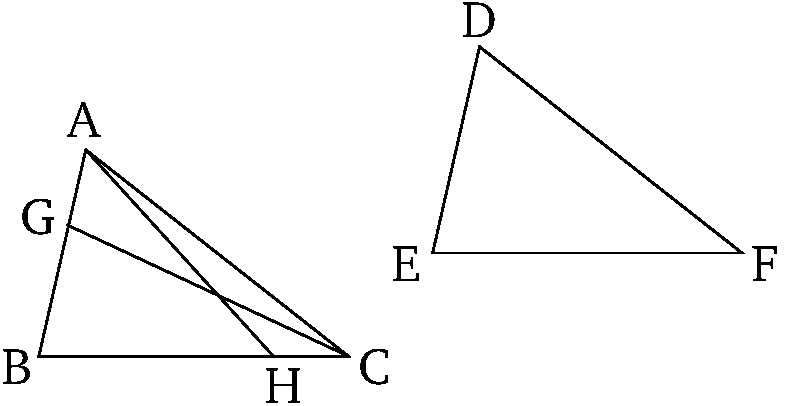
\includegraphics[width=0.8\textwidth]{Book01/fig26e.pdf}}

But, again, let the sides subtending the equal angles be equal: for instance, 
(let) $AB$ (be equal) to
$DE$.  Again, I say that the remaining sides will be equal to the remaining
sides. (That is) $AC$ (equal) to $DF$, and $BC$ to $EF$. Furthermore, the remaining angle
$BAC$ is equal to the remaining angle $EDF$.

For if $BC$ is unequal to $EF$ (then) one of them is greater. If possible, let $BC$
be greater. And let $BH$ be made equal to $EF$ [Prop.~1.3], and let $AH$ be joined.
And since $BH$ is equal to $EF$, and $AB$ to $DE$, the two (straight-lines) $AB$, $BH$
are equal to the two (straight-lines) $DE$, $EF$, respectively. And the angles
they encompass (are also equal). Thus, the base $AH$ is equal to the base  
$DF$, and the triangle $ABH$ is equal to the triangle $DEF$, and the
remaining angles subtended by the equal sides will be equal to the
(corresponding) remaining angles [Prop.~1.4]. Thus, angle $BHA$ 
is equal to $EFD$. But, $EFD$ is equal to $BCA$. So, in triangle $AHC$,
the external angle $BHA$ is equal to the internal and opposite angle 
$BCA$. The very thing (is) impossible [Prop.~1.16]. Thus, $BC$ is not unequal to $EF$.
Thus, (it is) equal. And $AB$ is also equal to $DE$. So the two
(straight-lines) $AB$, $BC$ are equal to the two (straight-lines) $DE$, $EF$,
respectively. And they encompass equal angles. Thus, the base $AC$ is equal
to the base $DF$, and triangle $ABC$ (is) equal to triangle $DEF$, and the
remaining angle $BAC$ (is) equal to the remaining angle $EDF$ [Prop.~1.4].

Thus, if two triangles have two angles equal to two angles, respectively, 
and one side equal to one side---in fact, either that by the equal angles, or that
subtending one of the equal angles---(then the triangles) will also have the remaining sides equal to the (corresponding) remaining sides, and the
remaining angle (equal) to the remaining angle. (Which is) the very thing it
was required to show.}
\end{Parallel}
\noindent{\footnotesize $^\dag$ The Greek text has ``$BG$, $BC$'', which is obviously a mistake.}

%%%%%%
% Prop 1.27
%%%%%%
\pdfbookmark[1]{Proposition 1.27}{pdf1.27}
\begin{Parallel}{}{} 
\ParallelLText{
\begin{center}
{\large \ggn{27}.}
\end{center}\vspace*{-7pt}

\gr{Ἐὰν εἰξ δύο εὐθείας εὐθεῖα ἐμπίπτουσα τὰξ ἐναλλὰχ γωνίας ἴσας ἀλλήλαις ποιῆ|, παράλληλοιὸέσονται ἀλλήλαις αἱ εὐθεῖαι.}

% Removed epsf size command
\centerline{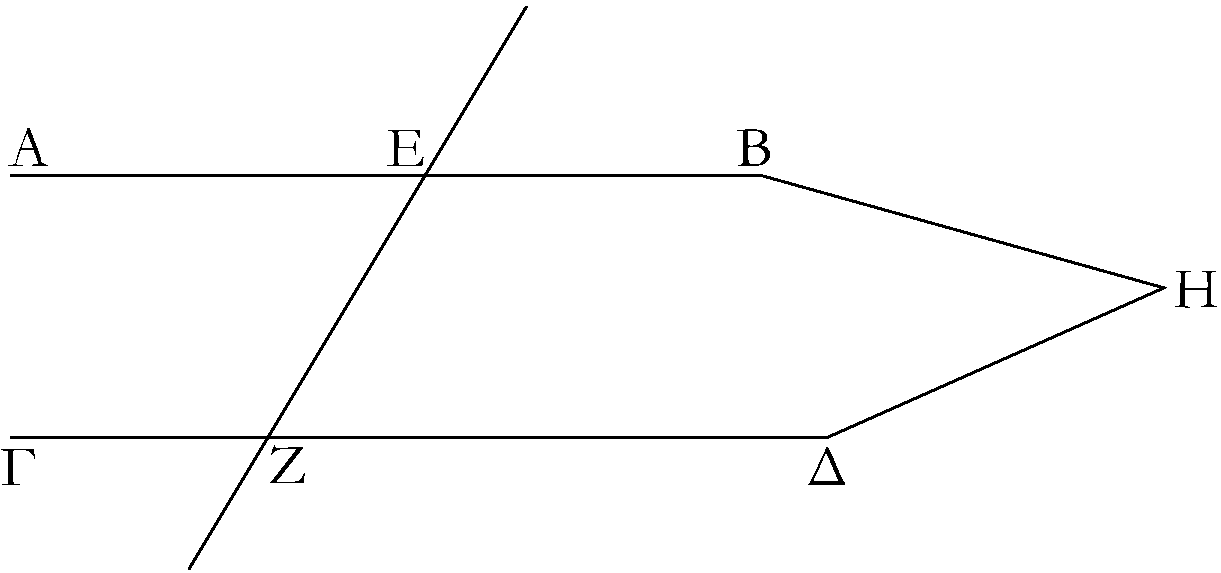
\includegraphics[width=0.8\textwidth]{Book01/fig27g.pdf}}

\gr{Εἰξ γὰρ δύο εὐθείας τὰξ ΑΒ, ΓΔ εὐθεῖα ἐμπίπτουσα ἡ ΕΖ τὰξ ἐναλλὰχ γωνίας τὰξ ὑπὸ ΑΕΖ, ΕΖΔ ἴσας ἀλλήλαις ποιείτω; λέγω, ὅτι
παράλληλόξ ἐστιν ἡ ΑΒ τῇ ΓΔ.}

\gr{Εἰ γὰρ μή, ἐκβαλλόμεναι αἱ ΑΒ, ΓΔ συμπεσοῦνται ἢτοι ἐπὶ τὰ Β, Δ μέρηὸὴ  ἐπὶ τὰ  Α, Γ. ἐκβεβλήσθωσαν καὶ συμπιπτέτωσαν ἐπὶ τὰ Β, Δ μέρη κατὰ τὸ Η.  τριγώνου δὴ τοῦ ΗΕΖ ἡ ἐκτὸξ γωνία ἡ ὑπὸ
ΑΕΖὸίση ἐστὶ τῇ ἐντὸς καὶ ἀπεναντίον τῇ ὑπὸ ΕΖΗ;
ὅπερ ἐστὶν ἀδύνατον; οὐκ ἄρα αἱ ΑΒ, ΔΓ ἐκβαλλόμεναι
συμπεσοῦνται ἐπὶ τὰ Β, Δ μέρη. ὁμοίως δὴ δειθθήσεται, ὅτι οὐδὲ ἐπὶ τὰ Α, Γ; αἱ δὲ ἐπὶ μ  ηδέτερα τὰ μέρη συμπίπτουσαι παράλληλοί
εἰσιν; παράλληλος ἄρα ἐστὶν ἡ ΑΒ τῇ ΓΔ.}

\gr{Ἐὰν ἄρα εἰξ δύο εὐθείας εὐθεῖα ἐμπίπτουσα τὰξ ἐναλλὰχ γωνίας ἴσας ἀλλήλαις ποιῆ|, παράλληλοιὸέσονται αἱ εὐθεῖαι;
ὅπερ ἔδει δεῖχαι.}}

\ParallelRText{
\begin{center}
{\large Proposition 27}
\end{center}

If a straight-line falling across two straight-lines makes  the alternate
angles equal to one another (then) the (two) straight-lines will be parallel to
one another.

% Removed epsf size command
\centerline{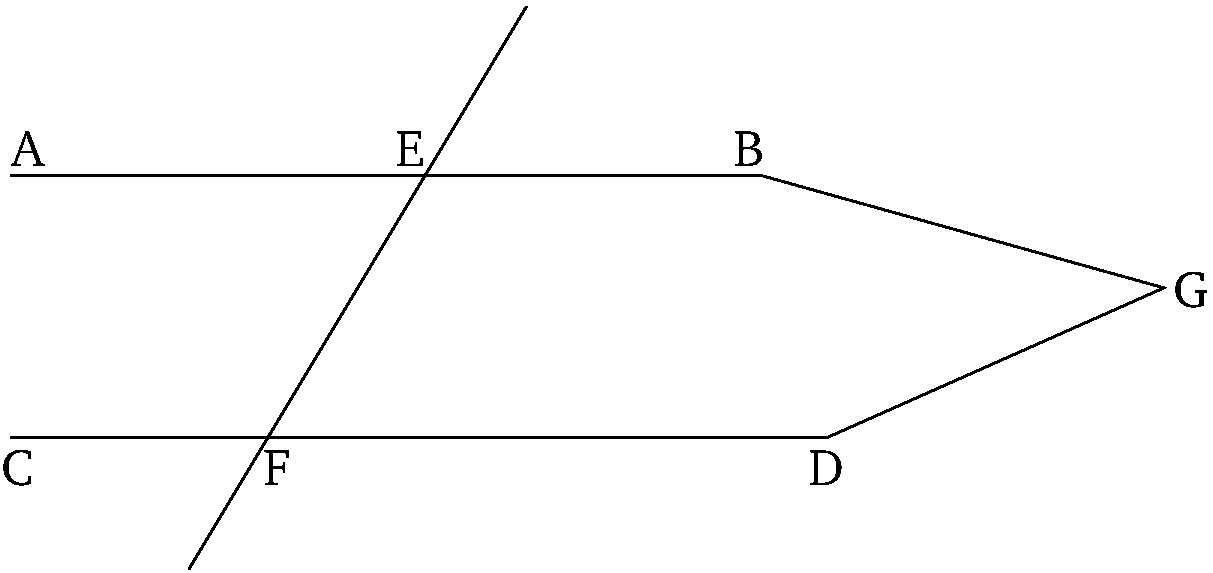
\includegraphics[width=0.8\textwidth]{Book01/fig27e.pdf}}

For let the straight-line $EF$, falling across the two straight-lines $AB$ and
$CD$, make the alternate angles $AEF$ and $EFD$ equal to one another.
I say that $AB$ and $CD$ are parallel.

For if not, being produced, $AB$ and $CD$ will certainly meet together:
either in the direction of $B$ and $D$, or (in the
direction) of $A$ and $C$ [Def.~1.23]. Let them be
produced, and let them meet together in the direction of $B$ and $D$ at
 (point) $G$. So, for the triangle $GEF$, the external angle
$AEF$ is equal to the interior and opposite (angle) $EFG$. The
very thing is impossible [Prop.~1.16]. Thus, being produced, $AB$ and $CD$
will not meet together in the direction of $B$ and $D$. Similarly, 
it can be shown that neither (will they meet together) in (the
direction of) $A$ and $C$. But  (straight-lines) meeting in neither
direction are parallel [Def.~1.23]. Thus, $AB$ and $CD$ are parallel.

Thus, if a straight-line falling across two straight-lines makes  the alternate
angles equal to one another (then) the (two) straight-lines will be parallel (to
one another). (Which is) the very thing it was required to show.}
\end{Parallel}

%%%%%%
% Prop 1.28
%%%%%%
\pdfbookmark[1]{Proposition 1.28}{pdf1.28}
\begin{Parallel}{}{} 
\ParallelLText{
\begin{center}
{\large \ggn{28}.}
\end{center}\vspace*{-7pt}

\gr{Ἐὰν εἰξ δύο εὐθείας εὐθεῖα ἐμπίπτουσα τὴν ἐκτὸξ γωνίαν τῇ ἐντὸς καὶ ἀπεναντίον καὶ ἐπὶ τὰ αὐτὰ μέρη ἴσην ποιῆ| ὸὴ τὰξ ἐντὸς καὶ ἐπὶ τὰ αὐτὰ μέρη δυσὶν ὀρθαῖξ ἴσας, παράλληλοιὸέσονται ἀλλήλαις αἱ εὐθεῖαι.}

\gr{Εἰξ γὰρ δύο εὐθείας τὰξ ΑΒ, ΓΔ εὐθεῖα ἐμπίπτουσα ἡ ΕΖ τὴν ἐκτὸξ γωνίαν τὴν ὑπὸ ΕΗΒ τῇ ἐντὸς καὶ ἀπεναντίον γωνίᾳ
τῇ ὑπὸ ΗΘΔ ἴσην ποιείτωὸὴ τὰξ ἐντὸς καὶ ἐπὶ τὰ αὐτὰ μέρη
τὰξ ὑπὸ ΒΗΘ, ΗΘΔ δυσὶν ὀρθαῖξ ἴσας; λέγω, ὅτι παράλληλόξ ἐστιν
ἡ ΑΒ τῇ ΓΔ.}

\gr{Ἐπεὶ γὰρὸίση ἐστὶν ἡ ὑπὸ ΕΗΒ τῇ ὑπὸ ΗΘΔ, ἀλλὰ ἡ ὑπὸ
ΕΗΒ τῇ ὑπὸ ΑΗΘ ἐστινὸίση, καὶ ἡ ὑπὸ ΑΗΘ ἄρα τῇ ὑπὸ ΗΘΔ
ἐστινὸίση; καί εἰσιν ἐναλλάχ; παράλληλος ἄρα ἐστὶν
ἡ ΑΒ τῇ ΓΔ.}

\gr{Πάλιν, ἐπεὶ αἱ ὑπὸ ΒΗΘ, ΗΘΔ δύο ὀρθαῖξ ἴσαι εἰσίν, εἰσὶ
δὲ καὶ αἱ ὑπὸ ΑΗΘ, ΒΗΘ δυσὶν ὀρθαῖξ ἴσαι, αἱ  ἄρα ὑπὸ ΑΗΘ, ΒΗΘ
ταῖς ὑπὸ ΒΗΘ, ΗΘΔ ἴσαι εἰσίν; κοινὴ ἀφῃρήσθω ἡ ὑπὸ ΒΗΘ;
λοιπὴ  ἄρα ἡ ὑπὸ ΑΗΘ λοιπῆ| τῇ ὑπὸ ΗΘΔ ἐστινὸίση;
καί εἰσιν ἐναλλάχ; παράλληλος ἄρα ἐστὶν ἡ ΑΒ τῇ ΓΔ.}\\~\\

% Removed epsf size command
\centerline{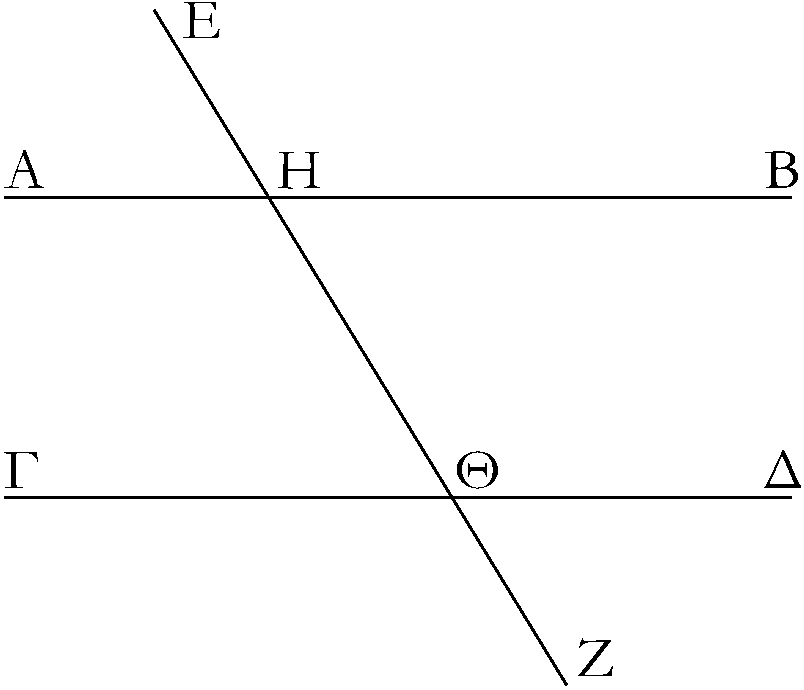
\includegraphics[width=0.8\textwidth]{Book01/fig28g.pdf}}

\gr{Ἐὰν ἄρα εἰξ δύο εὐθείας εὐθεῖα ἐμπίπτουσα τὴν ἐκτὸξ γωνίαν τῇ ἐντὸς καὶ ἀπεναντίον καὶ ἐπὶ τὰ αὐτὰ μέρη ἴσην ποιῆ| ὸὴ τὰξ ἐντὸς καὶ ἐπὶ τὰ αὐτὰ μέρη δυσὶν ὀρθαῖξ ἴσας, παράλληλοιὸέσονται  αἱ εὐθεῖαι; ὅπερ ἔδει δεῖχαι.}}

\ParallelRText{
\begin{center}
{\large Proposition 28}
\end{center}

If a straight-line falling across two straight-lines makes the external angle equal
to the internal and opposite angle on the same side, or (makes) the (sum  of the) internal
(angles) on the same side equal
to two right-angles, (then) the (two) straight-lines will be parallel to
one another.

For let $EF$, falling across the two straight-lines $AB$ and $CD$, make the external
angle $EGB$ equal to the internal and opposite angle $GHD$, or the (sum of the) internal
(angles) on the same side, $BGH$ and $GHD$, equal to two right-angles.
I say that $AB$ is parallel to $CD$.

For since (in the first case) $EGB$ is equal to $GHD$, but $EGB$ is equal to $AGH$ [Prop.~1.15],
$AGH$ is thus also equal to $GHD$. And they are alternate (angles).
Thus, $AB$ is
 parallel to $CD$ [Prop.~1.27].

Again, since (in the second case, the sum of) $BGH$ and $GHD$ is equal to two right-angles,  and (the sum of) $AGH$ and
$BGH$ is also equal to two right-angles [Prop.~1.13], 
(the sum of) $AGH$ and $BGH$ is thus equal to (the sum of) $BGH$ and $GHD$. Let $BGH$ be
subtracted from both. Thus, the remainder $AGH$ is equal to the remainder
$GHD$. And they are alternate (angles). Thus, $AB$ is parallel
to $CD$ [Prop.~1.27].

% Removed epsf size command
\centerline{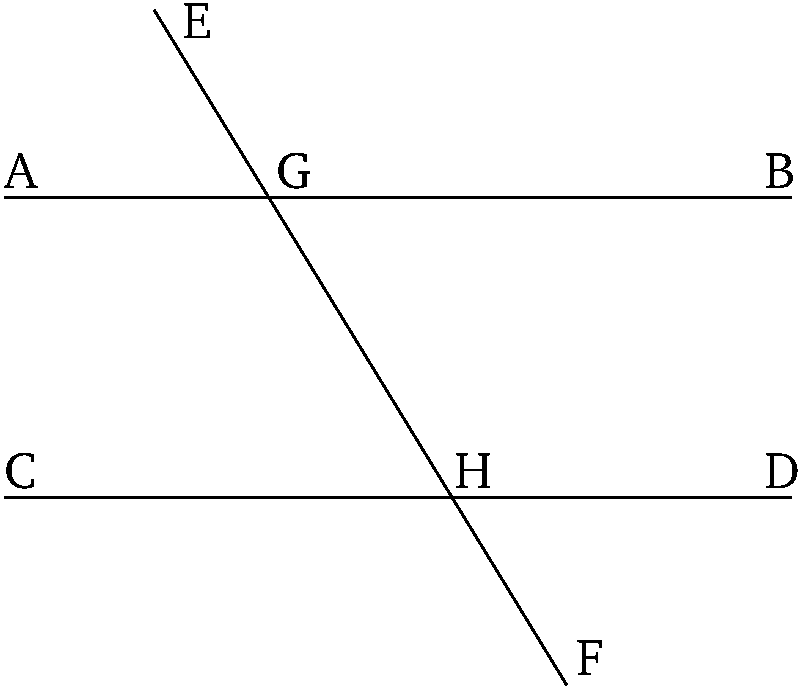
\includegraphics[width=0.8\textwidth]{Book01/fig28e.pdf}}

Thus, if a straight-line falling across  two straight-lines makes the external angle equal
to the internal and opposite angle on the same side, or (makes) the (sum of the) internal
(angles) on the same side equal
to two right-angles, (then) the (two) straight-lines will be parallel (to
one another). (Which is) the very thing it was required to show.}
\end{Parallel}

%%%%%%
% Prop 1.29
%%%%%%
\pdfbookmark[1]{Proposition 1.29}{pdf1.29}
\begin{Parallel}{}{} 
\ParallelLText{
\begin{center}
{\large\ggn{29}.}
\end{center}\vspace*{-7pt}

\gr{Ἡ εἰξ τὰξ παραλλήλους εὐθείας εὐθεῖα ἐμπίπτουσα τάξ τε ἐναλλὰχ γωνίας ἴσας ἀλλήλαις ποιεῖ καὶ τὴν ἐκτὸξ τῇ ἐντὸς καὶ ἀπεναντίον ἴσην καὶ τὰξ ἐντὸς καὶ ἐπὶ τὰ αὐτὰ μέρη δυσὶν ὀρθαῖξ ἴσας.}

\gr{Εἰξ γὰρ παραλλήλους εὐθείας τὰξ ΑΒ, ΓΔ εὐθεῖα ἐμπιπτέτω ἡ ΕΖ;
λέγω, ὅτι τὰξ ἐναλλὰχ γωνίας τὰξ ὑπὸ ΑΗΘ, ΗΘΔ ἴσας ποιεῖ καὶ τὴν ἐκτὸξ γωνίαν τὴν ὑπὸ ΕΗΒ τῇ ἐντὸς καὶ ἀπεναντίον τῇ ὑπὸ ΗΘΔ ἴσην καὶ τὰξ ἐντὸς καὶ ἐπὶ τὰ αὐτὰ μέρη τὰξ ὑπὸ ΒΗΘ, ΗΘΔ δυσὶν ὀρθαῖξ ἴσας.}\\

\gr{Εἰ γὰρὸάνισόξ ἐστιν ἡ ὑπὸ ΑΗΘ τῇ ὑπὸ ΗΘΔ, μία αὐτῶν μείζων ἐστίν. ὸέστω μείζων ἡ ὑπὸ ΑΗΘ; κοινὴ προσκείσθω ἡ ὑπὸ ΒΗΘ; αἱ  ἄρα ὑπὸ ΑΗΘ, ΒΗΘ τῶν ὑπὸ ΒΗΘ, ΗΘΔ μείζονέξ εἰσιν. ἀλλὰ αἱ ὑπὸ ΑΗΘ, ΒΗΘ δυσὶν ὀρθαῖξ ἴσαι εἰσίν. [καὶ] αἱ  ἄρα ὑπὸ ΒΗΘ, ΗΘΔ δύο ὀρθῶν ἐλάσσονέξ εἰσιν. αἱ δὲ ἀπὸ ἐλασσόνωνὸὴ δύο ὀρθῶν ἐκβαλλόμεναι εἰξ ἄπειρον συμπίπτουσιν; αἱ  ἄρα ΑΒ, ΓΔ ἐκβαλλόμεναι εἰξ ἄπειρον συμπεσοῦνται; οὐ συμπίπτουσι δὲ διὰ τὸ παραλλήλους αὐτὰξ ὑποκεῖσθαι; οὐκ ἄραὸάνισόξ ἐστιν ἡ ὑπὸ 
ΑΗΘ τῇ ὑπὸ ΗΘΔ; ὸίση ἄρα. ἀλλὰ ἡ ὑπὸ ΑΗΘ τῇ ὑπὸ ΕΗΒ ἐστινὸίση;
καὶ ἡ ὑπὸ ΕΗΒ ἄρα τῇ ὑπὸ ΗΘΔ ἐστινὸίση;
κοινὴ προσκείσθω ἡ ὑπὸ ΒΗΘ; αἱ  ἄρα ὑπὸ ΕΗΒ, ΒΗΘ ταῖς
ὑπὸ ΒΗΘ, ΗΘΔ ἴσαι εἰσίν. ἀλλὰ αἱ ὑπὸ ΕΗΒ, ΒΗΘ δύο ὀρθαῖξ ἴσαι εἰσίν; καὶ αἱ ὑπὸ ΒΗΘ, ΗΘΔ ἄρα δύο ὀρθαῖξ ἴσαι
εἰσίν.}\\~\\~\\

% Removed epsf size command
\centerline{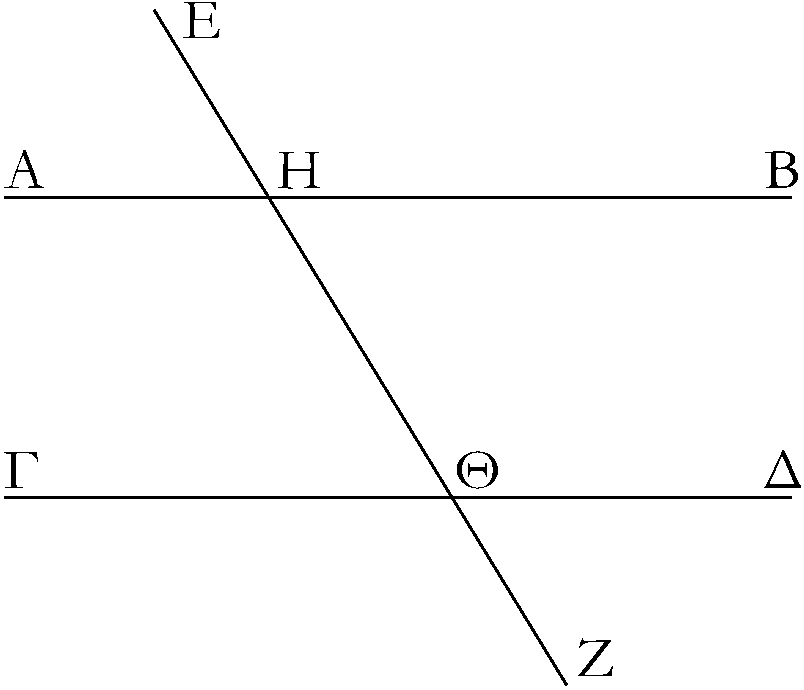
\includegraphics[width=0.8\textwidth]{Book01/fig28g.pdf}}

\gr{Ἡ   ἄρα εἰξ τὰξ παραλλήλους εὐθείας εὐθεῖα ἐμπίπτουσα τάξ τε ἐναλλὰχ γωνίας ἴσας ἀλλήλαις ποιεῖ καὶ τὴν ἐκτὸξ τῇ ἐντὸς καὶ ἀπεναντίον ἴσην καὶ τὰξ ἐντὸς καὶ ἐπὶ τὰ αὐτὰ μέρη δυσὶν ὀρθαῖξ ἴσας;
ὅπερ ἔδει δεῖχαι.}}

\ParallelRText{
\begin{center}
{\large Proposition 29}
\end{center}

A straight-line falling across  parallel straight-lines makes the alternate angles
equal to one another,  the external (angle) equal to the internal and
opposite (angle), and the (sum of the) internal (angles) on the same side equal to
two right-angles.

For let the straight-line $EF$ fall across the parallel straight-lines $AB$ and $CD$.
I say that it makes the  alternate angles, $AGH$ and $GHD$,  equal,  the
external angle $EGB$ equal to the internal and opposite (angle) $GHD$,
and the (sum of the) internal (angles) on the same side, $BGH$ and $GHD$, equal to
two right-angles.

For if $AGH$ is unequal to $GHD$ (then) one of them is greater. Let $AGH$ be greater.
Let $BGH$ be added to both. Thus, (the sum of) $AGH$ and $BGH$ is greater
than (the sum of) $BGH$ and $GHD$. But, (the sum of) $AGH$ and $BGH$ is equal to two right-angles
[Prop~1.13]. Thus,  (the sum of) $BGH$ and $GHD$ is [also] less than two right-angles. 
But (straight-lines) being produced to infinity from (internal angles whose sum is) less than
two right-angles meet together [Post.~5]. Thus, $AB$ and $CD$, being produced to
infinity, will meet together. But they do not meet, on account of
them (initially) being assumed parallel (to one another) [Def.~1.23]. Thus, $AGH$ is not unequal to $GHD$. Thus, (it is) equal. But, $AGH$ is equal to $EGB$ [Prop.~1.15]. 
And $EGB$ is thus also equal to $GHD$.
Let $BGH$
be added to both. Thus, (the sum of) $EGB$ and $BGH$ is equal to (the sum of) $BGH$ and $GHD$.
But, (the sum of) $EGB$ and $BGH$ is equal to two right-angles [Prop.~1.13]. 
Thus, (the sum of) $BGH$ and $GHD$ is also equal to two right-angles.

% Removed epsf size command
\centerline{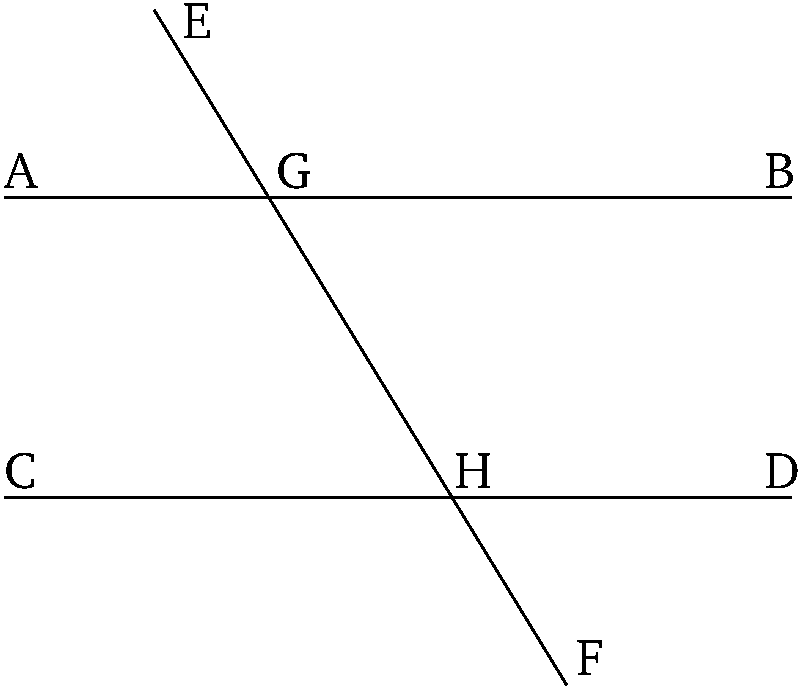
\includegraphics[width=0.8\textwidth]{Book01/fig28e.pdf}}

Thus, a straight-line falling across parallel straight-lines makes the alternate angles
equal to one another,  the external (angle) equal to the internal and
opposite (angle), and the (sum of the) internal (angles) on the same side equal to
two right-angles. (Which is) the very thing it was required to show.}
\end{Parallel}

%%%%%%
% Prop 1.30
%%%%%%
\pdfbookmark[1]{Proposition 1.30}{pdf1.30}
\begin{Parallel}{}{} 
\ParallelLText{
\begin{center}
{\large \ggn{30}.}
\end{center}\vspace*{-7pt}

\gr{Αἱ τῇ αὐτῇ εὐθείᾳ παράλληλοι καὶ ἀλλήλαις εἰσὶ παράλληλοι.}

\gr{Ἔστω ἑκατέρα τῶν ΑΒ, ΓΔ τῇ ΕΖ παράλληλος; λέγω, ὅτι καὶ ἡ ΑΒ τῇ ΓΔ ἐστι παράλληλος.}

\gr{Ἐμπιπτέτω γὰρ εἰξ αὐτὰξ εὐθεῖα ἡ ΗΚ.}

% Removed epsf size command
\centerline{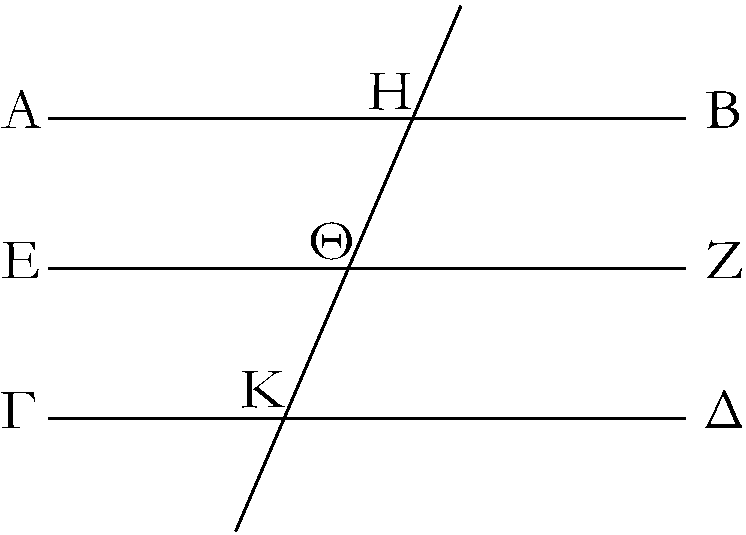
\includegraphics[width=0.8\textwidth]{Book01/fig30g.pdf}}

\gr{Καὶ ἐπεὶ εἰξ παραλλήλους εὐθείας τὰξ ΑΒ, ΕΖ εὐθεῖα ἐμπέπτωκεν ἡ ΗΚ, ὸίση ἄρα ἡ ὑπὸ ΑΗΚ τῇ ὑπὸ ΗΘΖ. πάλιν, ἐπεὶ εἰξ παραλλήλους εὐθείας τὰξ ΕΖ, ΓΔ εὐθεῖα ἐμπέπτωκεν ἡ ΗΚ, ὸίση ἐστὶν ἡ ὑπὸ ΗΘΖ τῇ ὑπὸ ΗΚΔ. ἐδείθθη δὲ καὶ ἡ ὑπὸ ΑΗΚ
τῇ ὑπὸ ΗΘΖὸίση. καὶ ἡ ὑπὸ ΑΗΚ ἄρα τῇ ὑπὸ ΗΚΔ ἐστινὸίση; καί εἰσιν ἐναλλάχ. παράλληλος ἄρα ἐστὶν ἡ ΑΒ τῇ ΓΔ.}

\gr{[Αἱ   ἄρα τῇ αὐτῇ εὐθείᾳ παράλληλοι καὶ ἀλλήλαις εἰσὶ παράλληλοι;]
ὅπερ ἔδει δεῖχαι.}}

\ParallelRText{
\begin{center}
{\large Proposition 30}
\end{center}

(Straight-lines) parallel to the same straight-line are also parallel
to one another.

Let each of the (straight-lines) $AB$ and $CD$ be parallel to $EF$. I say that
$AB$ is also parallel to $CD$.

For let the straight-line $GK$ fall across  ($AB$, $CD$, and $EF$).

% Removed epsf size command
\centerline{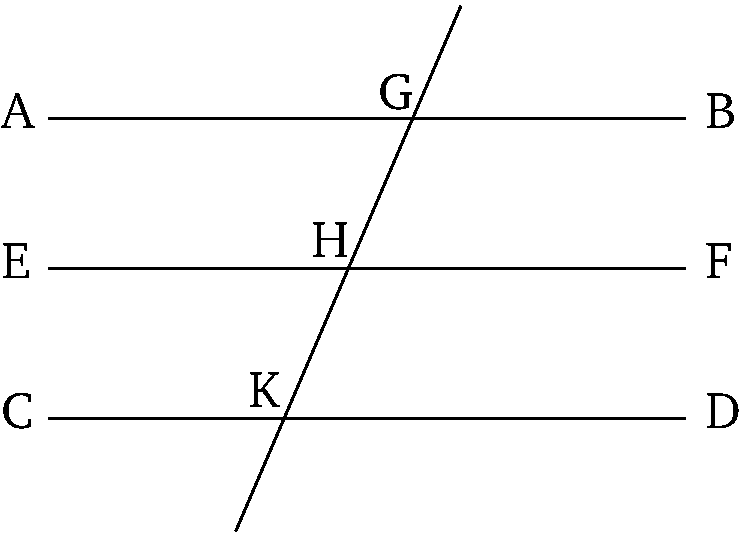
\includegraphics[width=0.8\textwidth]{Book01/fig30e.pdf}}

And since the straight-line $GK$ has fallen across the parallel straight-lines $AB$ and $EF$, (angle) $AGK$
(is) thus equal to $GHF$ [Prop.~1.29]. Again, since the straight-line $GK$ has fallen across the parallel
straight-lines $EF$ and $CD$, (angle) $GHF$ is equal to $GKD$ [Prop.~1.29].
But $AGK$ was also shown (to be) equal to $GHF$. Thus, $AGK$ is also equal to 
$GKD$. And they are alternate (angles). Thus, $AB$ is parallel to $CD$ [Prop.~1.27].

\mbox{[}Thus, (straight-lines) parallel to the same straight-line are also parallel
to one another.] (Which is) the very thing it was required to show.}
\end{Parallel}

%%%%%%
% Prop 1.31
%%%%%%
\pdfbookmark[1]{Proposition 1.31}{pdf1.31}
\begin{Parallel}{}{} 
\ParallelLText{
\begin{center}
{\large \ggn{31}.}
\end{center}\vspace*{-7pt}

\gr{Διὰ τοῦ δοθέντος σημείου τῇ δοθείσῃ εὐθείᾳ παράλληλον εὐθεῖαν
γραμμὴν ἀγαγεῖν.}

\gr{Ἔστω τὸ μὲν δοθὲν σημεῖον τὸ Α, ἡ δὲ δοθεῖσα εὐθεῖα ἡ ΒΓ;
δεῖ δὴ διὰ τοῦ Α σημείου τῇ ΒΓ εὐθείᾳ παράλληλον εὐθεῖαν γραμμὴν ἀγαγεῖν.}

\gr{Εἰλήφθω ἐπὶ τῆς ΒΓ τυθὸν σημεῖον τὸ Δ, καὶ ἐπεζεύθθω ἡ ΑΔ; καὶ συνεστάτω πρὸς τῇ ΔΑ εὐθείᾳ καὶ τῷ πρὸς αὐτῇ σημείῳ  
 τῷ Α τῇ ὑπὸ ΑΔΓ γωνίᾳ ὸίση ἡ ὑπὸ ΔΑΕ; καὶ ἐκβεβλήσθω ἐπ' εὐθείας τῇ ΕΑ εὐθεῖα ἡ ΑΖ.}\\
 
% Removed epsf size command
\centerline{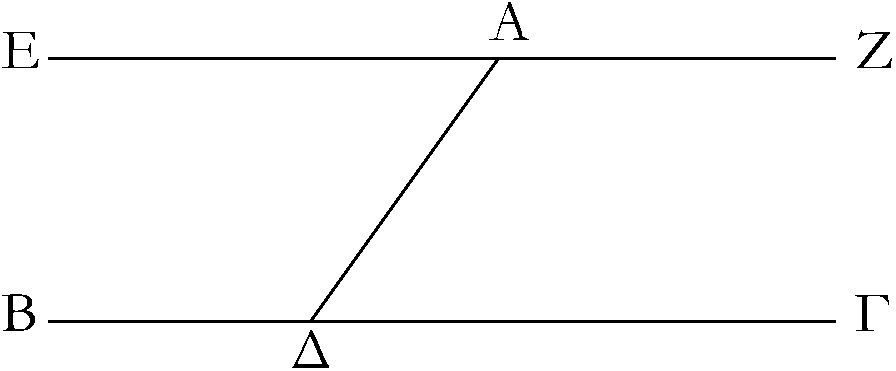
\includegraphics[width=0.8\textwidth]{Book01/fig31g.pdf}}
 
\gr{Καὶ ἐπεὶ εἰξ δύο εὐθείας τὰξ ΒΓ, ΕΖ εὐθεῖα ἐμπίπτουσα ἡ
ΑΔ τὰξ ἐναλλὰχ γωνίας τὰξ ὑπὸ ΕΑΔ, ΑΔΓ ἴσας ἀλλήλαις πεποίηκεν, παράλληλος ἄρα ἐστὶν ἡ ΕΑΖ τῇ ΒΓ.}

\gr{Διὰ τοῦ δοθέντος ἄρα σημείου τοῦ Α τῇ δοθείσῃ εὐθείᾳ τῇ ΒΓ παράλληλος εὐθεῖα
γραμμὴ ὸῆκται ἡ ΕΑΖ; ὅπερ ἔδει ποιῆσαι.}}

\ParallelRText{
\begin{center}
{\large Proposition 31}
\end{center}

To draw a straight-line parallel to a given straight-line, through a given
point.

Let $A$ be the given point, and $BC$ the given straight-line. So it is
required to draw a straight-line parallel to the straight-line $BC$, through
the point $A$.

Let the point $D$ be taken a random  on $BC$, and let $AD$ be
joined. And let (angle) $DAE$, equal to angle $ADC$,  be constructed 
on the straight-line $DA$ at the point $A$ on it [Prop.~1.23]. And let the
straight-line $AF$ be
produced in a straight-line with $EA$.

% Removed epsf size command
\centerline{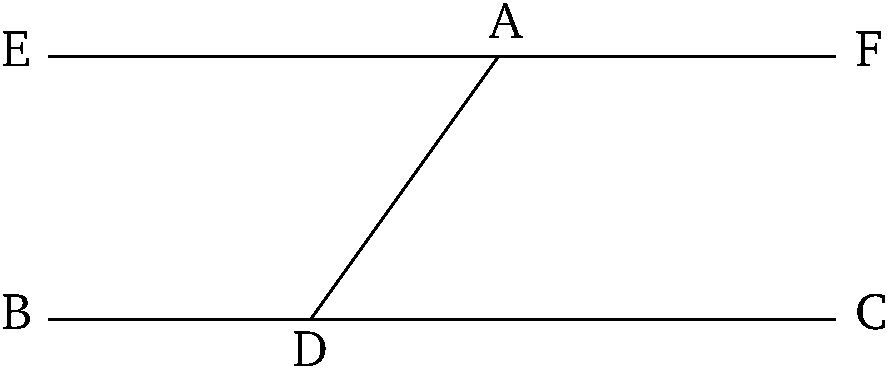
\includegraphics[width=0.8\textwidth]{Book01/fig31e.pdf}}

And since the straight-line $AD$, (in) falling across the two straight-lines
$BC$ and $EF$,  has made the alternate
angles $EAD$ and $ADC$ equal to one another, $EAF$ is thus parallel to $BC$
[Prop.~1.27].

Thus, the straight-line $EAF$ has been drawn parallel to the given straight-line $BC$, through the  given
point $A$. (Which is) the very thing it was required to do.}
\end{Parallel}

%%%%%%
% Prop 1.32
%%%%%%
\pdfbookmark[1]{Proposition 1.32}{pdf1.32}
\begin{Parallel}{}{} 
\ParallelLText{
\begin{center}
{\large \ggn{32}.}
\end{center}\vspace*{-7pt}

\gr{Παντὸξ τριγώνου μιᾶς τῶν πλευρῶν προσεκβληθείσης ἡ ἐκτὸξ γωνία
δυσὶ ταῖς ἐντὸς καὶ ἀπεναντίονὸίση ἐστίν, καὶ αἱ ἐντὸς τοῦ τριγώνου τρεῖς γωνίαι δυσὶν ὀρθαῖξ ἴσαι εἰσίν.}~\\

% Removed epsf size command
\centerline{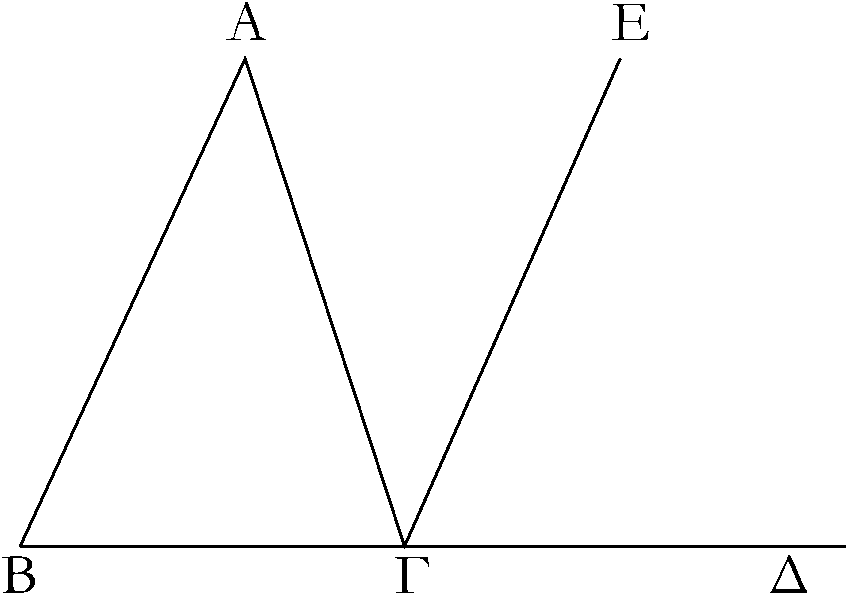
\includegraphics[width=0.8\textwidth]{Book01/fig32g.pdf}}

\gr{Ἔστω τρίγωνον τὸ ΑΒΓ, καὶ προσεκβεβλήσθω αὐτοῦ μία πλευρὰ ἡ ΒΓ
ἐπὶ τὸ Δ; λέγω, ὅτι ἡ ἐκτὸξ γωνία ἡ ὑπὸ ΑΓΔὸίση ἐστὶ δυσὶ ταῖς ἐντὸς καὶ ἀπεναντίον ταῖς ὑπὸ ΓΑΒ, ΑΒΓ, καὶ αἱ ἐντὸς
τοῦ τριγώνου
 τρεῖς γωνίαι αἱ ὑπὸ ΑΒΓ, ΒΓΑ, ΓΑΒ δυσὶν ὀρθαῖξ ἴσαι εἰσίν.}
 
 \gr{ὸ'Ηθθω γὰρ διὰ τοῦ Γ σημείου τῇ ΑΒ εὐθείᾳ παράλληλος ἡ ΓΕ.}
 
 \gr{Καὶ ἐπεὶ παράλληλόξ ἐστιν ἡ ΑΒ τῇ ΓΕ, καὶ εἰξ αὐτὰξ ἐμπέπτωκεν ἡ ΑΓ, αἱ ἐναλλὰχ γωνίαι αἱ ὑπὸ ΒΑΓ, ΑΓΕ ἴσαι ἀλλήλαις εἰσίν. πάλιν, ἐπεὶ παράλληλόξ ἐστιν ἡ ΑΒ τῇ ΓΕ, καὶ εἰξ αὐτὰξ ἐμπέπτωκεν εὐθεῖα ἡ ΒΔ, ἡ ἐκτὸξ γωνία ἡ ὑπὸ ΕΓΔὸίση ἐστὶ τῇ  ἐντὸς καὶ ἀπεναντίον τῇ ὑπὸ ΑΒΓ. ἐδείθθη δὲ καὶ ἡ ὑπὸ ΑΓΕ τῇ ὑπὸ ΒΑΓὸίση; ὅλη ἄρα ἡ ὑπὸ ΑΓΔ γωνίαὸίση ἐστὶ δυσὶ ταῖς ἐντὸς καὶ ἀπεναντίον ταῖς ὑπὸ ΒΑΓ, ΑΒΓ.}
 
 \gr{Κοινὴ προσκείσθω ἡ ὑπὸ ΑΓΒ; αἱ  ἄρα ὑπὸ ΑΓΔ, ΑΓΒ τρισὶ ταῖς ὑπὸ ΑΒΓ, ΒΓΑ, ΓΑΒ ἴσαι εἰσίν. ἀλλὸ αἱ ὑπὸ ΑΓΔ, ΑΓΒ δυσὶν ὀρθαῖξ ἴσαι εἰσίν; καὶ αἱ ὑπὸ ΑΓΒ, ΓΒΑ, ΓΑΒ ἄρα δυσὶν ὀρθαῖξ ἴσαι εἰσίν.}
 
 \gr{Παντὸξ ἄρα τριγώνου μιᾶς τῶν πλευρῶν προσεκβληθείσης ἡ ἐκτὸξ γωνία
δυσὶ ταῖς ἐντὸς καὶ ἀπεναντίονὸίση ἐστίν, καὶ αἱ ἐντὸς τοῦ τριγώνου τρεῖς γωνίαι δυσὶν ὀρθαῖξ ἴσαι εἰσίν; ὅπερ ἔδει
δεῖχαι.}}

\ParallelRText{
\begin{center}
{\large Proposition 32}
\end{center}

In any triangle,  (if) one of the sides (is) produced  (then) the external
angle is equal to the (sum of the) two internal and opposite (angles), and the (sum of the) three
internal angles of the triangle is equal to two right-angles.

% Removed epsf size command
\centerline{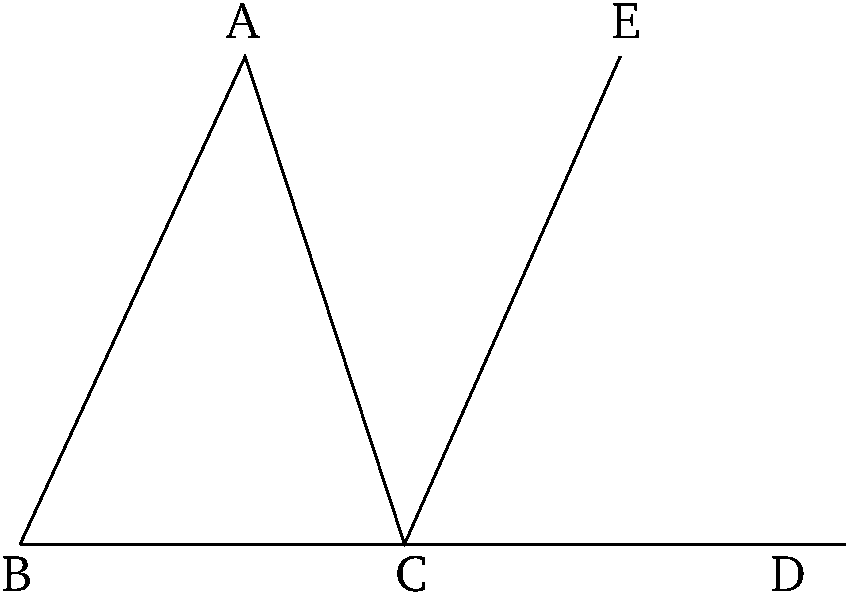
\includegraphics[width=0.8\textwidth]{Book01/fig32e.pdf}}

Let $ABC$ be a triangle, and let one of its sides $BC$ be produced to $D$.
I say that the external angle $ACD$ is equal to the (sum of the) two internal and opposite
angles $CAB$ and $ABC$, and the (sum of the) three internal angles of the triangle---$ABC$, $BCA$, and $CAB$---is equal to two right-angles.

For let $CE$ be drawn through point $C$ parallel to the straight-line
$AB$ [Prop.~1.31].

And since $AB$ is parallel to $CE$, and $AC$ has fallen across them, the alternate
angles $BAC$ and $ACE$ are equal to one another [Prop.~1.29]. Again,
since $AB$ is parallel to $CE$, and the straight-line $BD$ has fallen across them, 
the external angle $ECD$ is equal to the internal and opposite (angle)
$ABC$ [Prop.~1.29]. But $ACE$ was also shown (to be) equal to $BAC$. Thus, the whole
angle $ACD$ is equal to the (sum of the) two internal and opposite (angles) $BAC$ and $ABC$.

Let $ACB$ be added to both. Thus, (the sum of) $ACD$ and $ACB$ is equal to
the (sum of the) three (angles) $ABC$, $BCA$, and $CAB$. But, (the sum of) $ACD$ and $ACB$ is equal
to two right-angles [Prop.~1.13]. Thus, (the sum of) $ACB$, $CBA$, and $CAB$ is also
equal to two right-angles.

Thus, in any triangle,  (if) one of the sides  (is) produced (then) the external
angle is equal to the (sum of the) two internal and opposite (angles), and the (sum of the) three
internal angles of the triangle is equal to two right-angles. (Which is)
the very thing it was required to show.}
\end{Parallel}

%%%%%%
% Prop 1.33
%%%%%%
\pdfbookmark[1]{Proposition 1.33}{pdf1.33}
\begin{Parallel}{}{} 
\ParallelLText{
\begin{center}
{\large \ggn{33}.}
\end{center}\vspace*{-7pt}

\gr{Αἱ τὰξ ἴσας τε καὶ παραλλήλους ἐπὶ τὰ αὐτὰ μέρη ἐπιζευγνύουσαι εὐθεῖαι καὶ αὐταὶ  ἴσαι τε καὶ παράλληλοί εἰσιν.}

\gr{Ἔστωσαν ἴσαι τε καὶ παράλληλοι αἱ  ΑΒ, ΓΔ, καὶ ἐπιζευγνύτωσαν αὐτὰξ ἐπὶ τὰ αὐτὰ μέρη εὐθεῖαι αἱ ΑΓ, ΒΔ; λέγω, ὅτι καὶ αἱ ΑΓ, ΒΔ ἴσαι τε καὶ παράλληλοί εἰσιν.}

% Removed epsf size command
\centerline{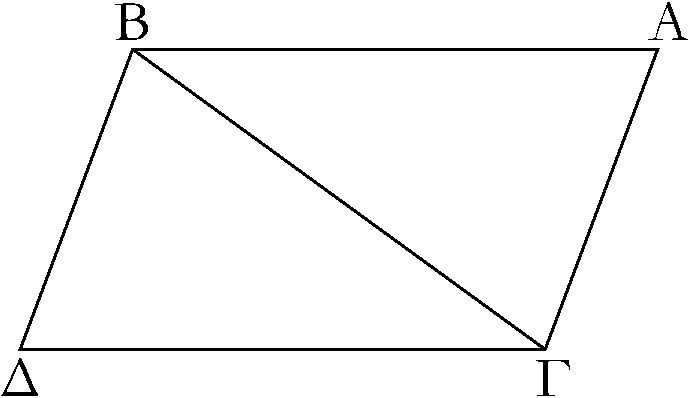
\includegraphics[width=0.8\textwidth]{Book01/fig33g.pdf}}

\gr{Ἐπεζεύθθω ἡ ΒΓ. καὶ ἐπεὶ παράλληλόξ ἐστιν ἡ ΑΒ τῇ ΓΔ, καὶ εἰξ αὐτὰξ ἐμπέπτωκεν ἡ ΒΓ, αἱ ἐναλλὰχ γωνίαι αἱ ὑπὸ ΑΒΓ, ΒΓΔ ἴσαι ἀλλήλαις εἰσίν. καὶ ἐπεὶ ὸίση ἐστὶν ἡ ΑΒ τῇ ΓΔ κοινὴ δὲ ἡ
ΒΓ, δύο δὴ αἱ ΑΒ, ΒΓ δύο ταῖς
 ΒΓ, ΓΔ ἴσαι εἰσίν; καὶ γωνία ἡ ὑπὸ ΑΒΓ γωνίᾳ τῇ ὑπὸ ΒΓΔὸίση; βάσις ἄρα ἡ ΑΓ βάσει τῇ ΒΔ ἐστινὸίση, καὶ τὸ ΑΒΓ τρίγωνον τῷ ΒΓΔ τριγώνῳ  ἴσον ἐστίν, καὶ αἱ λοιπαὶ γωνίαι ταῖς λοιπαῖξ γωνίαις ἴσαιὸέσονται ἑκατέρα ἑκατέρᾳ, ὑφὸ ὁὰξ αἱ  ἴσαι πλευραὶ
ὑποτείνουσιν; ὸίση ἄρα ἡ ὑπὸ ΑΓΒ γωνία τῇ ὑπὸ ΓΒΔ. καὶ
ἐπεὶ εἰξ δύο εὐθείας τὰξ ΑΓ, ΒΔ εὐθεῖα
ἐμπίπτουσα ἡ ΒΓ τὰξ ἐναλλὰχ γωνίας ἴσας ἀλλήλαις πεποίηκεν, παράλληλος ἄρα ἐστὶν ἡ ΑΓ τῇ ΒΔ. ἐδείθθη δὲ αὐτῇ καὶ ὸίση.}

\gr{Αἱ  ἄρα τὰξ ἴσας τε καὶ παραλλήλους ἐπὶ τὰ αὐτὰ μέρη ἐπιζευγνύουσαι εὐθεῖαι καὶ αὐταὶ  ἴσαι τε καὶ παράλληλοί εἰσιν;
 ὅπερ ἔδει
δεῖχαι.}}

\ParallelRText{
\begin{center}
{\large Proposition 33}
\end{center}

Straight-lines joining equal and parallel (straight-lines) on the same sides
are  themselves also equal and parallel.

Let $AB$ and $CD$ be equal and parallel (straight-lines), and let the
straight-lines $AC$ and $BD$ join them on the same sides. I say that $AC$
and $BD$ are also equal and parallel.

% Removed epsf size command
\centerline{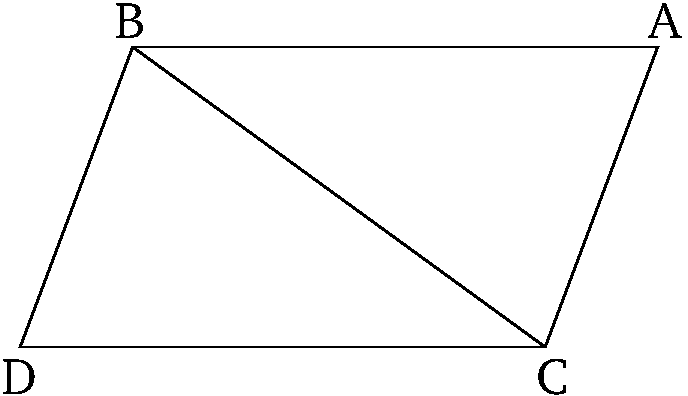
\includegraphics[width=0.8\textwidth]{Book01/fig33e.pdf}}

Let $BC$ be joined. And since $AB$ is parallel to $CD$, and $BC$ has
fallen across them, the alternate angles $ABC$ and $BCD$ are equal to one another [Prop.~1.29]. And since $AB$ is equal to $CD$, and $BC$ is common,
the two (straight-lines) $AB$, $BC$ are equal to the two (straight-lines)
$DC$, $CB$.$^\dag$And the angle $ABC$ is equal to the angle $BCD$. Thus, the
base $AC$ is equal to the base $BD$, and triangle $ABC$ is equal to triangle
$DCB$$^\ddag$, and the remaining angles will be equal to the corresponding remaining
angles subtended by the equal sides [Prop.~1.4]. Thus,  angle $ACB$ 
is equal to $CBD$. Also, since the straight-line $BC$, (in) falling across the two
straight-lines $AC$ and $BD$, has made the alternate angles  ($ACB$ and $CBD$) equal to one another,
$AC$ is thus parallel to $BD$ [Prop.~1.27]. And ($AC$) was also shown (to be) equal
to ($BD$).

Thus, straight-lines joining equal and parallel (straight-lines) on the same sides
are  themselves also equal and parallel. (Which is) the very thing it was
required to show.}
\end{Parallel}
{\footnotesize \noindent$^\dag$ The Greek text has ``$BC$, $CD$'', which is obviously a mistake.} \\
{\footnotesize \noindent$^\ddag$ The Greek text has ``$DCB$'', which is obviously a mistake.} 

%%%%%%
% Prop 1.34
%%%%%%
\pdfbookmark[1]{Proposition 1.34}{pdf1.34}
\begin{Parallel}{}{} 
\ParallelLText{
\begin{center}
{\large \ggn{34}.}
\end{center}\vspace*{-7pt}

\gr{Τῶν παραλληλογράμμων θωρίων αἱ ἀπεναντίον πλευραί τε καὶ γωνίαι ἴσαι ἀλλήλαις εἰσίν, καὶ ἡ διάμετρος αὐτὰ δίθα τέμνει.}

\gr{Ἔστω παραλληλόγραμμον θωρίον τὸ ΑΓΔΒ, διάμετρος δὲ αὐτοῦ ἡ ΒΓ; λέγω, ὅτι τοῦ ΑΓΔΒ παραλληλογράμμου αἱ ἀπεναντίον πλευραί τε καὶ γωνίαι ἴσαι ἀλλήλαις εἰσίν, καὶ ἡ ΒΓ διάμετρος αὐτὸ δίθα τέμνει.}

% Removed epsf size command
\centerline{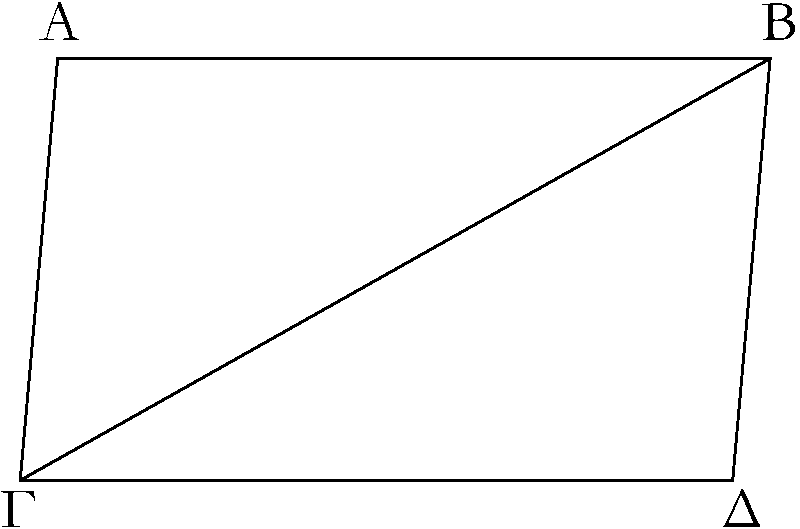
\includegraphics[width=0.8\textwidth]{Book01/fig34g.pdf}}

\gr{Ἐπεὶ γὰρ παράλληλόξ ἐστιν ἡ ΑΒ τῇ ΓΔ, καὶ εἰξ αὐτὰξ ἐμπέπτωκεν
εὐθεῖα ἡ ΒΓ, αἱ ἐναλλὰχ γωνίαι αἱ ὑπὸ ΑΒΓ, ΒΓΔ ἴσαι ἀλλήλαις εἰσίν. πάλιν ἐπεὶ παράλληλόξ ἐστιν ἡ ΑΓ τῇ ΒΔ, καὶ εἰξ αὐτὰξ ἐμπέπτωκεν ἡ ΒΓ, αἱ ἐναλλὰχ γωνίαι αἱ ὑπὸ ΑΓΒ, ΓΒΔ ἴσαι ἀλλήλαις εἰσίν. δύο δὴ τρίγωνά ἐστι τὰ ΑΒΓ, ΒΓΔ τὰξ δύο γωνίας τὰξ ὑπὸ ΑΒΓ, ΒΓΑ δυσὶ ταῖς ὑπὸ ΒΓΔ, ΓΒΔ ἴσας ἔχοντα ἑκατέραν ἑκατέρᾳ καὶ μίαν πλευρὰν μιᾶ| πλευρᾶ|  ἴσην τὴν πρὸς ταῖς ἴσαις γωνίαις κοινὴν αὐτῶν τὴν ΒΓ; καὶ τὰξ λοιπὰξ ἄρα πλευρὰξ ταῖς λοιπαῖξ ἴσας ὁέχει ἑκατέραν ἑκατέρᾳ καὶ τὴν λοιπὴν γωνίαν τῇ λοιπῆ| γωνίᾳ; ὸίση ἄρα ἡ μὲν ΑΒ πλευρὰ τῇ ΓΔ, ἡ δὲ ΑΓ τῇ ΒΔ, καὶ ὸέτιὸίση ἐστὶν ἡ ὑπὸ ΒΑΓ γωνία τῇ ὑπὸ ΓΔΒ. καὶ ἐπεὶ ὸίση ἐστὶν ἡ μὲν ὑπὸ ΑΒΓ γωνία τῇ ὑπὸ ΒΓΔ, ἡ δὲ ὑπὸ ΓΒΔ τῇ ὑπὸ ΑΓΒ, ὅλη ἄρα ἡ ὑπὸ ΑΒΔ ὅλῃ τῇ ὑπὸ ΑΓΔ ἐστινὸίση. ἐδείθθη δὲ καὶ ἡ ὑπὸ ΒΑΓ τῇ ὑπὸ ΓΔΒὸίση.}

\gr{Τῶν ἄρα παραλληλογράμμων θωρίων αἱ ἀπεναντίον πλευραί τε
καὶ γωνίαι ἴσαι ἀλλήλαις εἰσίν.}

\gr{Λέγω δή, ὅτι καὶ ἡ διάμετρος αὐτὰ δίθα τέμνει. ἐπεὶ γὰρὸίση ἐστὶν ἡ ΑΒ τῇ ΓΔ, κοινὴ δὲ ἡ ΒΓ, δύο δὴ αἱ ΑΒ, ΒΓ δυσὶ ταῖς ΓΔ, ΒΓ ἴσαι εἰσὶν ἑκατέρα ἑκατέρᾳ; καὶ γωνία ἡ ὑπὸ ΑΒΓ γωνίᾳ τῇ ὑπὸ ΒΓΔὸίση. καὶ βάσις ἄρα ἡ ΑΓ τῇ ΔΒὸίση. καὶ τὸ ΑΒΓ [ ἄρα] τρίγωνον τῷ ΒΓΔ τριγώνῳ  ἴσον ἐστίν.}

\gr{Ἡ  ἄρα ΒΓ διάμετρος δίθα τέμνει τὸ ΑΒΓΔ παραλληλόγραμμον;
ὅπερ ἔδει δεῖχαι.}}

\ParallelRText{
\begin{center}
{\large Proposition 34}
\end{center}
In parallelogramic figures, the opposite sides and angles are equal to one
another, and a diagonal cuts them in half.

Let $ACDB$ be a parallelogramic figure, and $BC$ its diagonal. I say that
for parallelogram $ACDB$, the opposite sides and angles are equal to
one another, and the diagonal $BC$ cuts it in half.\\

% Removed epsf size command
\centerline{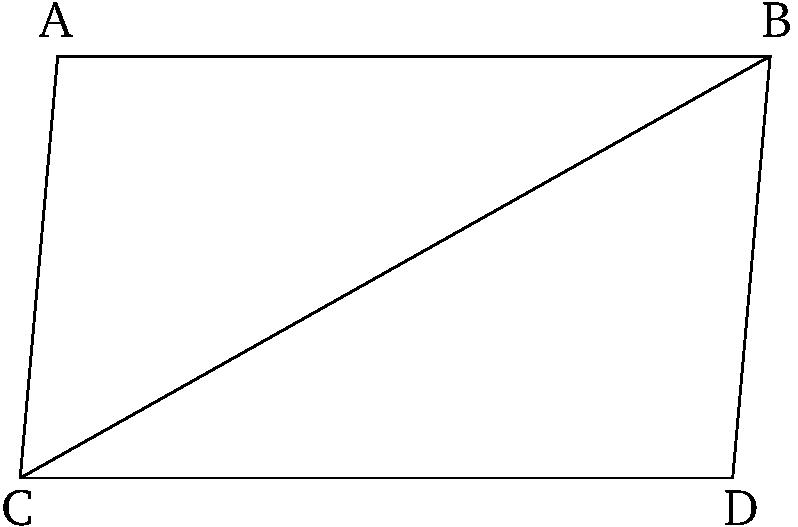
\includegraphics[width=0.8\textwidth]{Book01/fig34e.pdf}}

For since $AB$ is parallel to $CD$, and the straight-line $BC$ has fallen
across  them, the alternate angles $ABC$ and $BCD$ are equal to one another [Prop.~1.29]. 
Again, since $AC$ is parallel to $BD$, and $BC$ has fallen across them, the
alternate angles $ACB$ and $CBD$ are equal to one another [Prop.~1.29]. 
So $ABC$ and $BCD$ are two triangles having the two angles $ABC$ and
$BCA$ equal to the two (angles) $BCD$ and $CBD$, respectively, and one
side equal to one side---the (one) by the equal angles and common to them, (namely) $BC$. Thus,
they will also  have the remaining sides  equal to the corresponding
remaining (sides), and the remaining angle (equal) to the remaining angle [Prop.~1.26].
Thus, side $AB$ is equal to $CD$, and $AC$ to $BD$. Furthermore, angle $BAC$ is 
equal to $CDB$. And since angle $ABC$ is equal to $BCD$, and $CBD$ to
$ACB$, the whole (angle) $ABD$ is thus equal to the whole (angle) $ACD$.
And  $BAC$ was also shown  (to be) equal to $CDB$.

Thus, in parallelogramic figures, the opposite sides and angles are equal
to one another.

And, I also say that a diagonal cuts them in half. For since $AB$ is equal
to $CD$, and $BC$ (is) common, the two (straight-lines) $AB$, $BC$ are equal
to the two (straight-lines) $DC$, $CB$$^\dag$, respectively. And angle $ABC$ is
equal to angle $BCD$. Thus, the base $AC$ (is) also equal to $DB$, and
triangle $ABC$ is equal to triangle $BCD$ [Prop.~1.4].

Thus, the diagonal $BC$ cuts the parallelogram $ACDB$$^\ddag$ in half. (Which is) the
very thing it was required to show.}
\end{Parallel}
{\footnotesize \noindent$^\dag$ The Greek text has ``$CD$, $BC$'',
which is obviously a mistake.\\
$^\ddag$ The Greek
text has ``$ABCD$'', which is obviously a mistake.}

%%%%%%
% Prop 1.35
%%%%%%
\pdfbookmark[1]{Proposition 1.35}{pdf1.35}
\begin{Parallel}{}{} 
\ParallelLText{
\begin{center}
{\large \ggn{35}.}
\end{center}\vspace*{-7pt}

\gr{Τὰ παραλληλόγραμμα τὰ ἐπὶ τῆς αὐτῆς βάσεως ὅντα καὶ ἐν ταῖς
αὐταῖς παραλλήλοις ἴσα ἀλλήλοις ἐστίν.}

\gr{Ἔστω παραλληλόγραμμα τὰ ΑΒΓΔ, ΕΒΓΖ ἐπὶ τῆς αὐτῆς βάσεως τῆς
ΒΓ καὶ ἐν ταῖς αὐταῖς παραλλήλοις ταῖς ΑΖ, ΒΓ; λέγω, ὅτι ἴσον ἐστὶ τὸ ΑΒΓΔ τῷ ΕΒΓΖ παραλληλογράμμῳ.}

% Removed epsf size command
\centerline{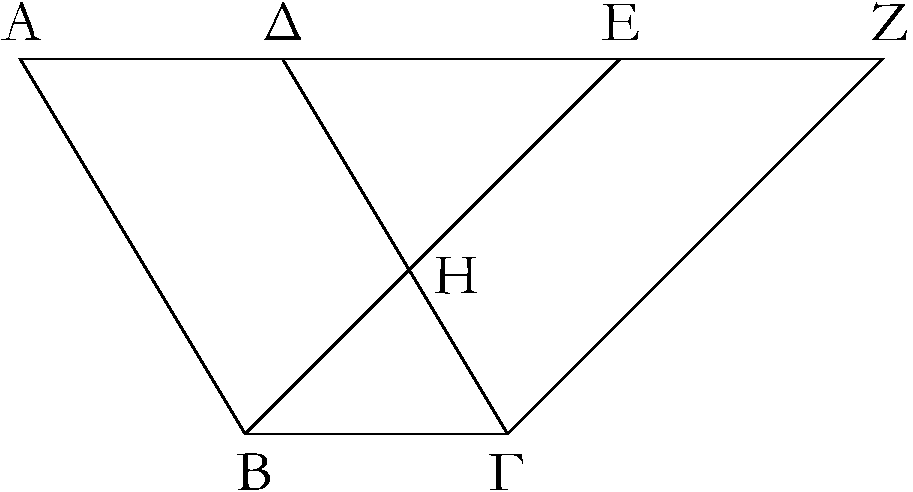
\includegraphics[width=0.8\textwidth]{Book01/fig35g.pdf}}

\gr{Ἐπεὶ γὰρ παραλληλόγραμμόν ἐστι τὸ ΑΒΓΔ, ὸίση ἐστὶν ἡ ΑΔ τῇ ΒΓ. διὰ τὰ αὐτὰ δὴ καὶ ἡ ΕΖ τῇ ΒΓ ἐστινὸίση; ὁώστε καὶ ἡ ΑΔ τῇ ΕΖ ἐστινὸίση; καὶ κοινὴ ἡ ΔΕ; ὅλη ἄρα ἡ ΑΕ ὅλῃ τῇ ΔΖ ἐστινὸίση. ὸέστι δὲ καὶ ἡ ΑΒ τῇ ΔΓὸίση; δύο δὴ αἱ ΕΑ, ΑΒ δύο ταῖς ΖΔ, ΔΓ ἴσαι εἰσὶν ἑκατέρα ἑκατέρᾳ; καὶ γωνία ἡ ὑπὸ ΖΔΓ γωνίᾳ
τῇ ὑπὸ ΕΑΒ ἐστινὸίση ἡ ἐκτὸξ τῇ ἐντόξ; βάσις ἄρα ἡ ΕΒ
βάσει τῇ ΖΓὸίση ἐστίν, καὶ τὸ ΕΑΒ τρίγωνον τῷ ΔΖΓ τριγώνῳ  ἴσονὸέσται; κοινὸν ἀφῃρήσθω τὸ ΔΗΕ; λοιπὸν ἄρα τὸ ΑΒΗΔ τραπέζιον λοιπῶ| τῷ ΕΗΓΖ τραπεζίῳ ἐστὶν ἴσον; κοινὸν προσκείσθω τὸ ΗΒΓ τρίγωνον; ὅλον ἄρα τὸ ΑΒΓΔ παραλληλόγραμμον ὅλῳ τῷ ΕΒΓΖ
παραλληλογράμμῳ  ἴσον ἐστίν.}

\gr{Τὰ  ἄρα παραλληλόγραμμα τὰ ἐπὶ τῆς αὐτῆς βάσεως ὅντα καὶ ἐν ταῖς
αὐταῖς παραλλήλοις ἴσα ἀλλήλοις ἐστίν; ὅπερ ἔδει δεῖχαι.}}

\ParallelRText{
\begin{center}
{\large Proposition 35}
\end{center}

Parallelograms which are on the same base and between the same
parallels are equal$^\dag$ to one another.

Let $ABCD$ and $EBCF$ be parallelograms on the same base $BC$, and
between the same parallels $AF$ and $BC$. I say that $ABCD$ is equal to
parallelogram $EBCF$.

% Removed epsf size command
\centerline{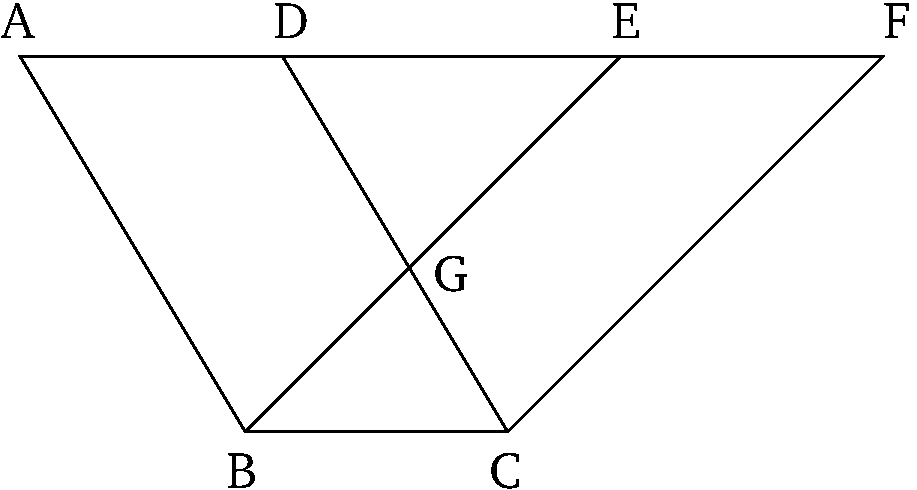
\includegraphics[width=0.8\textwidth]{Book01/fig35e.pdf}}

For since $ABCD$ is a parallelogram, $AD$ is equal to $BC$ [Prop.~1.34].
So, for the same (reasons), $EF$ is also equal to $BC$. So $AD$ is also equal to
$EF$. And $DE$ is common. Thus, the whole (straight-line) $AE$ is equal
to the whole (straight-line) $DF$.  And $AB$ is also equal to $DC$.
So the two (straight-lines) $EA$, $AB$
are equal to the two (straight-lines) $FD$, $DC$, respectively. And angle $FDC$ is
equal to angle $EAB$, the external to the internal [Prop.~1.29]. Thus, the
base $EB$ is equal to the base $FC$, and triangle $EAB$ will be equal to triangle
$DFC$ [Prop.~1.4]. Let $DGE$ be taken away from both. 
Thus, the remaining trapezium $ABGD$ is equal to the remaining trapezium
$EGCF$. Let triangle $GBC$ be added to both. Thus, the whole
parallelogram $ABCD$ is equal to the whole parallelogram $EBCF$.

Thus, parallelograms which are on the same base and between the same
parallels are equal to one another. (Which is) the very thing it was required to
show.}
\end{Parallel}
{\footnotesize \noindent$^\dag$ Here, for the first time, ``equal'' means
``equal in area'', rather than ``congruent''.}

%%%%%%
% Prop 1.36
%%%%%%
\pdfbookmark[1]{Proposition 1.36}{pdf1.36}
\begin{Parallel}{}{} 
\ParallelLText{
\begin{center}
{\large \ggn{36}.}
\end{center}\vspace*{-7pt}

\gr{Τὰ παραλληλόγραμμα τὰ ἐπὶ ὸίσων βάσεων ὅντα καὶ ἐν ταῖς αὐταῖς παραλλήλοις ἴσα ἀλλήλοις ἐστίν.}

\gr{Ἔστω παραλληλόγραμμα τὰ ΑΒΓΔ, ΕΖΗΘ ἐπὶ ὸίσων βάσεων ὅντα τῶν ΒΓ, ΖΗ καὶ ἐν ταῖς αὐταῖς παραλλήλοις ταῖς ΑΘ, ΒΗ; λέγω, ὅτι ἴσον ἐστὶ τὸ ΑΒΓΔ παραλληλόγραμμον τῷ ΕΖΗΘ.}

% Removed epsf size command
\centerline{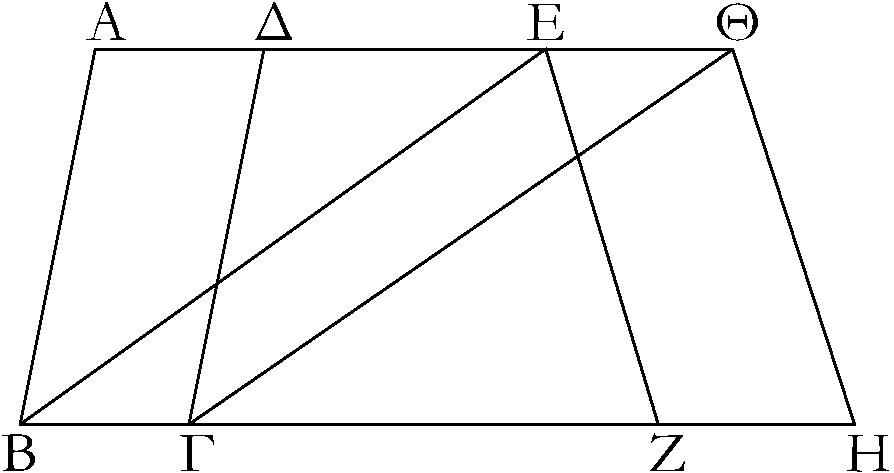
\includegraphics[width=0.8\textwidth]{Book01/fig36g.pdf}}

\gr{Ἐπεζεύθθωσαν γὰρ αἱ ΒΕ, ΓΘ. καὶ ἐπεὶ ὸίση ἐστὶν ἡ ΒΓ τῇ ΖΗ, ἀλλὰ ἡ ΖΗ τῇ ΕΘ ἐστινὸίση, καὶ ἡ ΒΓ ἄρα τῇ ΕΘ ἐστινὸίση.
εἰσὶ δὲ καὶ παράλληλοι. καὶ ἐπιζευγνύουσιν αὐτὰξ αἱ ΕΒ, ΘΓ; αἱ δὲ τὰξ ἴσας τε καὶ παραλλήλους ἐπὶ τὰ αὐτὰ μέρη ἐπιζευγνύουσαι ἴσαι
τε καὶ παράλληλοί εἰσι [καὶ αἱ ΕΒ, ΘΓ ἄρα ἴσαι τέ εἰσι καὶ παράλληλοι].
παραλληλόγραμμον ἄρα ἐστὶ τὸ ΕΒΓΘ. καί ἐστιν ἴσον τῷ ΑΒΓΔ; βάσιν τε γὰρ αὐτῷ τὴν αὐτὴν ἔχει τὴν ΒΓ, καὶ ἐν ταῖς αὐταῖς παραλλήλοις ἐστὶν αὐτῷ ταῖς ΒΓ, ΑΘ. δὶα τὰ αὐτὰ δὴ καὶ τὸ ΕΖΗΘ τῷ αὐτῷ τῷ ΕΒΓΘ ἐστιν ἴσον;
 ὁώστε καὶ τὸ ΑΒΓΔ παραλληλόγραμμον τῷ ΕΖΗΘ ἐστιν ἴσον.}
 
\gr{Τὰ   ἄρα παραλληλόγραμμα τὰ ἐπὶ ὸίσων βάσεων ὅντα καὶ ἐν ταῖς αὐταῖς παραλλήλοις ἴσα ἀλλήλοις ἐστίν; ὅπερ ἔδει δεῖχαι.}}

\ParallelRText{
\begin{center}
{\large Proposition 36}
\end{center}

Parallelograms which are on equal bases and between the same parallels are equal to one another.

Let $ABCD$ and $EFGH$ be parallelograms which are on the equal bases $BC$
and $FG$, and (are) between the same parallels $AH$ and $BG$. I say that
the parallelogram $ABCD$ is equal to $EFGH$.

% Removed epsf size command
\centerline{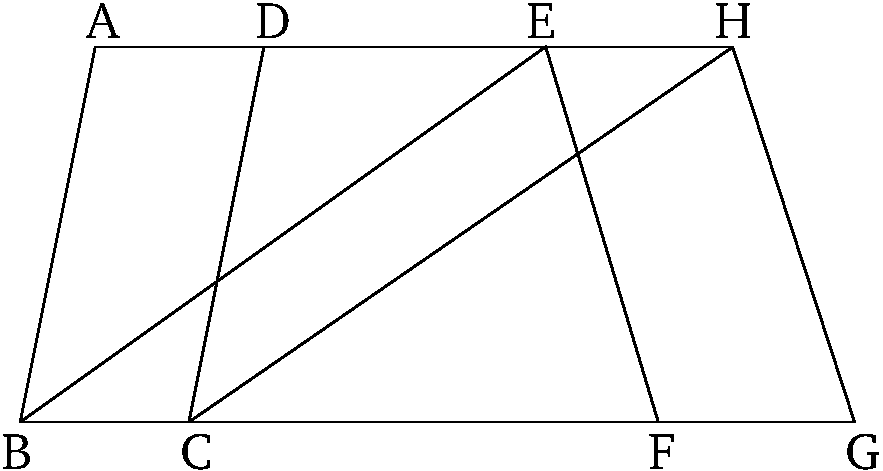
\includegraphics[width=0.8\textwidth]{Book01/fig36e.pdf}}

For let $BE$ and $CH$ be joined. And since $BC$ is equal to $FG$, but $FG$ is equal to $EH$ [Prop.~1.34], $BC$ is thus equal to $EH$. And they are also parallel, and $EB$ and $HC$ join them.
But (straight-lines) joining equal and parallel (straight-lines) on the
same sides are (themselves) equal and parallel [Prop.~1.33] [thus, $EB$ and $HC$
are also equal and parallel]. Thus, $EBCH$ is a parallelogram [Prop.~1.34],
and is equal to $ABCD$. For it has  the
same base, $BC$, (as $ABCD$), and is between the same parallels, $BC$ and $AH$, (as $ABCD$) [Prop.~1.35]. So,
for the same (reasons), $EFGH$ is also equal to the same (parallelogram) $EBCH$ [Prop.~1.34].  So that the
parallelogram $ABCD$ is  also equal to $EFGH$.

Thus, parallelograms which are on equal bases and between the same parallels are equal to one another. (Which is) the very thing it was required
to show.}
\end{Parallel}

%%%%%%
% Prop 1.37
%%%%%%
\pdfbookmark[1]{Proposition 1.37}{pdf1.37}
\begin{Parallel}{}{} 
\ParallelLText{
\begin{center}
{\large \ggn{37}.}
\end{center}\vspace*{-7pt}

\gr{Τὰ τρίγωνα τὰ ἐπὶ τῆς αὐτῆς βάσεως ὅντα καὶ ἐν ταῖς αὐταῖς
παραλλήλοις ἴσα ἀλλήλοις ἐστίν.}

\gr{Ἔστω τρίγωνα τὰ ΑΒΓ, ΔΒΓ ἐπὶ τῆς αὐτῆς βάσεως τῆς ΒΓ καὶ ἐν ταῖς αὐταῖς παραλλήλοις ταῖς ΑΔ, ΒΓ; λέγω, ὅτι ἴσον ἐστὶ τὸ ΑΒΓ τρίγωνον τῷ ΔΒΓ τριγώνῳ.}

% Removed epsf size command
\centerline{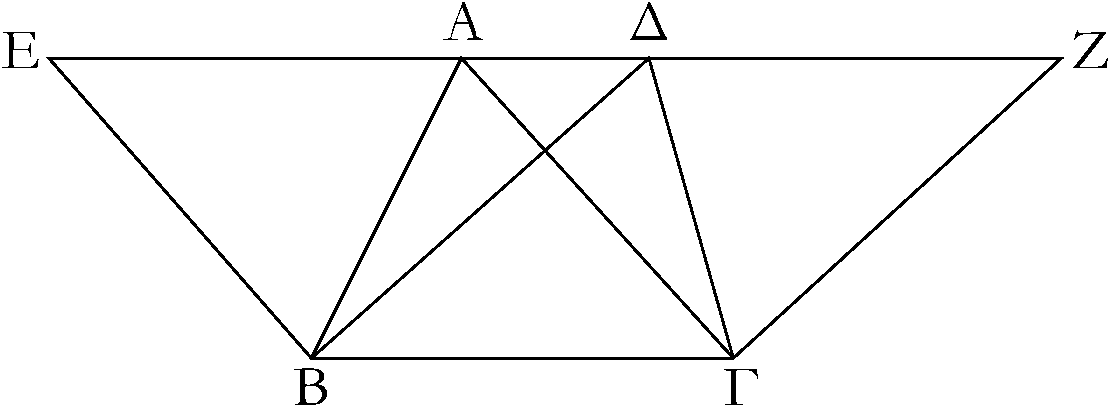
\includegraphics[width=0.8\textwidth]{Book01/fig37g.pdf}}

\gr{Ἐκβεβλήσθω ἡ ΑΔ ἐφ' ἑκάτερα τὰ μέρη ἐπὶ τὰ Ε, Ζ, καὶ διὰ μὲν τοῦ Β τῇ ΓΑ παράλληλος ἢθθω ἡ ΒΕ, δὶα δὲ τοῦ Γ τῇ ΒΔ παράλληλος ἢθθω ἡ ΓΖ.
 παραλληλόγραμμον ἄρα ἐστὶν ἑκάτερον τῶν ΕΒΓΑ, ΔΒΓΖ; καί εἰσιν ἴσα; ἐπί τε γὰρ τῆς αὐτῆς βάσεώξ εἰσι τῆς ΒΓ καὶ ἐν ταῖς αὐταῖς παραλλήλοις ταῖς ΒΓ, ΕΖ; καί ἐστι τοῦ μὲν ΕΒΓΑ
 παραλληλογράμμου
 ἥμισυ τὸ ΑΒΓ τρίγωνον; ἡ γὰρ ΑΒ διάμετρος αὐτὸ δίθα τέμνει; τοῦ δὲ ΔΒΓΖ παραλληλογράμμου ἥμισυ τὸ ΔΒΓ τρίγωνον; ἡ γὰρ ΔΓ διάμετρος αὐτὸ δίθα τέμνει. [τὰ δὲ τῶνὸίσων ἡμίση ἴσα 
 ἀλλήλοις ἐστίν].  ἴσον ἄρα ἐστὶ τὸ ΑΒΓ τρίγωνον τῷ ΔΒΓ τριγώνῳ.}
 
 \gr{Τὰ  ἄρα τρίγωνα τὰ ἐπὶ τῆς αὐτῆς βάσεως ὅντα καὶ ἐν ταῖς αὐταῖς
παραλλήλοις ἴσα ἀλλήλοις ἐστίν;  ὅπερ ἔδει δεῖχαι.}}

\ParallelRText{
\begin{center}
{\large Proposition 37}
\end{center}

Triangles which are on the same base and between the same parallels
are equal to one another.

Let $ABC$ and $DBC$ be triangles on the same base $BC$, and between
the same parallels $AD$ and $BC$. I say that triangle $ABC$ is equal to triangle $DBC$.

% Removed epsf size command
\centerline{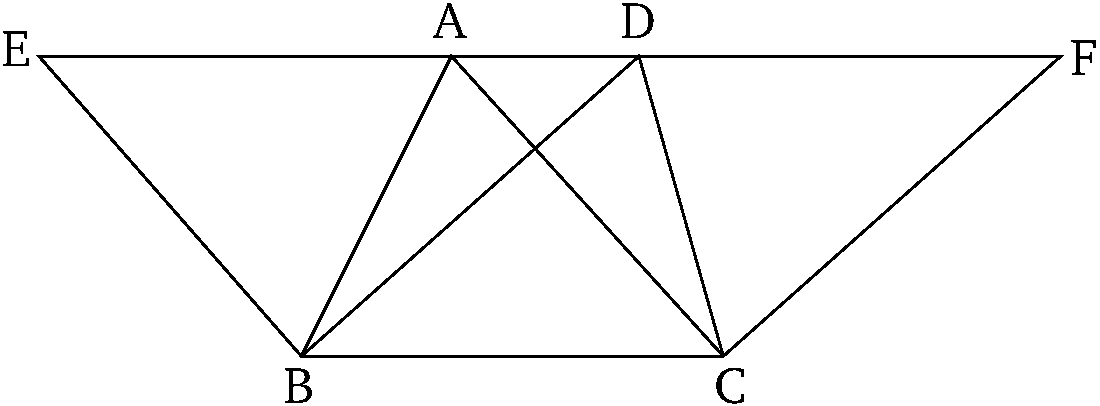
\includegraphics[width=0.8\textwidth]{Book01/fig37e.pdf}}

Let $AD$ be produced in both directions to $E$ and $F$, and let the
(straight-line) $BE$ be drawn through $B$ parallel to $CA$ [Prop.~1.31],
and let the (straight-line) $CF$ be drawn through $C$ parallel to
$BD$ [Prop.~1.31]. Thus, $EBCA$ and $DBCF$ are both parallelograms,
and are equal. For they are on the same base $BC$, and between
the same parallels $BC$ and $EF$ [Prop.~1.35]. And the triangle $ABC$ is
half of 
the parallelogram
$EBCA$. For the diagonal $AB$ cuts the latter in half [Prop.~1.34]. And the 
triangle $DBC$ (is) half of the parallelogram $DBCF$. For the diagonal
$DC$ cuts the latter in half [Prop.~1.34]. [And the halves of equal things are
equal to one another.]$^\dag$
Thus, triangle $ABC$ is equal to triangle $DBC$.

Thus, triangles which are on the same base and between the same parallels
are equal to one another. (Which is) the very thing it was required to show.}
\end{Parallel}
{\footnotesize \noindent$^\dag$ This is an additional common notion.}

%%%%%%
% Prop 1.38
%%%%%%
\pdfbookmark[1]{Proposition 1.38}{pdf1.38}
\begin{Parallel}{}{} 
\ParallelLText{
\begin{center}
{\large \ggn{38}.}
\end{center}\vspace*{-7pt}

\gr{Τὰ τρίγωνα τὰ ἐπὶ ὸίσων βάσεων ὅντα καὶ ἐν ταῖς αὐταῖς παραλλήλοις ἴσα ἀλλήλοις ἐστίν.}

\gr{Ἔστω τρίγωνα τὰ ΑΒΓ, ΔΕΖ ἐπὶ ὸίσων βάσεων τῶν ΒΓ, ΕΖ καὶ ἐν
ταῖς αὐταῖς παραλλήλοις ταῖς ΒΖ, ΑΔ; λέγω, ὅτι ἴσον ἐστὶ τὸ ΑΒΓ
τρίγωνον τῷ ΔΕΖ τριγώνῳ.}

% Removed epsf size command
\centerline{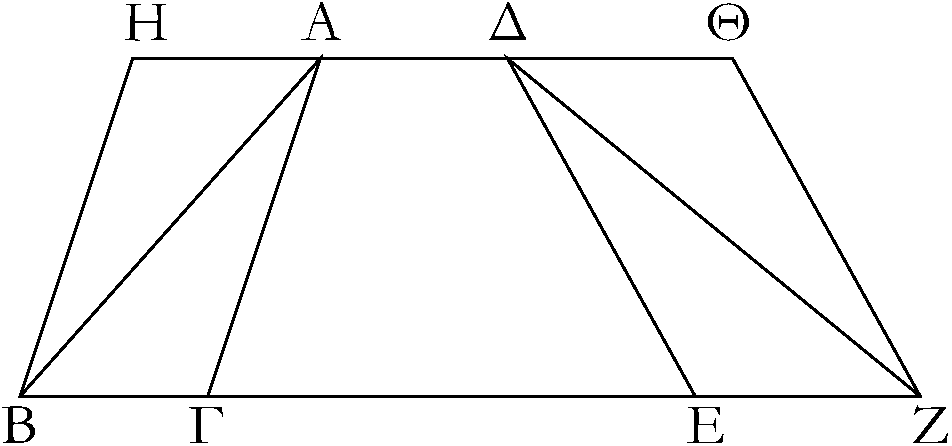
\includegraphics[width=0.8\textwidth]{Book01/fig38g.pdf}}

\gr{Ἐκβεβλήσθω γὰρ ἡ ΑΔ ἐφ' ἑκάτερα τὰ μέρη ἐπὶ τὰ Η, Θ, καὶ διὰ μὲν τοῦ Β τῇ ΓΑ παράλληλος ἢθθω ἡ ΒΗ, δὶα δὲ τοῦ Ζ τῇ ΔΕ
παράλληλος ἢθθω ἡ ΖΘ. παραλληλόγραμμον ἄρα ἐστὶν ἑκάτερον τῶν ΗΒΓΑ, ΔΕΖΘ; καὶ  ἴσον τὸ ΗΒΓΑ τῷ ΔΕΖΘ; ἐπί τε γὰρὸίσων βάσεών εἰσι τῶν ΒΓ, ΕΖ καὶ ἐν ταῖς αὐταῖς παραλλήλοις ταῖς ΒΖ, ΗΘ;
καί ἐστι τοῦ μὲν ΗΒΓΑ παραλληλογράμμου ἥμισυ τὸ ΑΒΓ τρίγωνον. ἡ γὰρ ΑΒ διάμετρος αὐτὸ δίθα τέμνει; τοῦ δὲ ΔΕΖΘ παραλληλογράμμου ἥμισυ τὸ ΖΕΔ τρίγωνον; ἡ γὰρ ΔΖ δίαμετρος
αὐτὸ δίθα τέμνει [τὰ δὲ τῶνὸίσων ἡμίση ἴσα ἀλλήλοις ἐστίν].
 ἴσον ἄρα ἐστὶ τὸ ΑΒΓ τρίγωνον τῷ ΔΕΖ τριγώνῳ.}

\gr{Τὰ  ἄρα τρίγωνα  τὰ ἐπὶ ὸίσων βάσεων ὅντα καὶ ἐν ταῖς αὐταῖς παραλλήλοις ἴσα ἀλλήλοις ἐστίν; ὅπερ ἔδει δεῖχαι.}}

\ParallelRText{
\begin{center}
{\large Proposition 38}
\end{center}

Triangles which are on equal bases and between the same parallels
are equal to one another.

Let $ABC$ and $DEF$ be triangles on the equal bases $BC$ and $EF$, and between the same parallels $BF$ and $AD$. I say that triangle $ABC$ is equal to triangle $DEF$.

% Removed epsf size command
\centerline{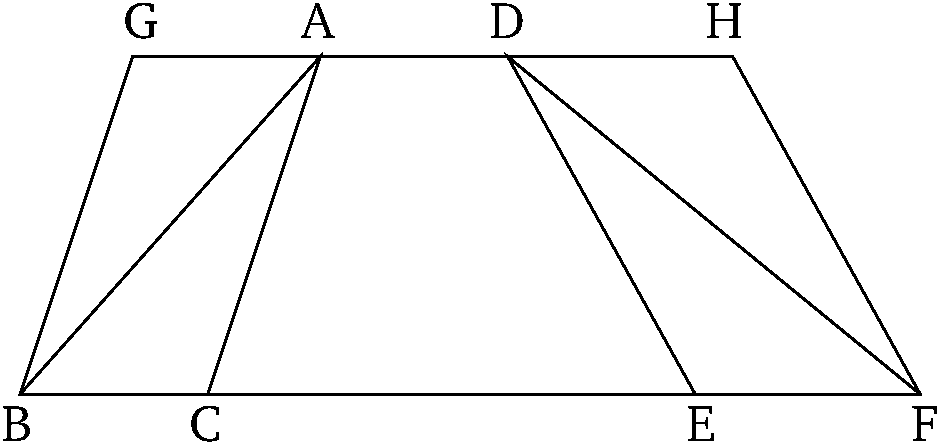
\includegraphics[width=0.8\textwidth]{Book01/fig38e.pdf}}

For let $AD$ be produced in both directions to $G$ and $H$, and
let the (straight-line) $BG$ be drawn through $B$ parallel to $CA$ [Prop.~1.31], and let the (straight-line) $FH$ be drawn through
$F$ parallel to $DE$ [Prop.~1.31]. Thus,  $GBCA$ and $DEFH$ are
each parallelograms. And $GBCA$ is equal to $DEFH$.
For they are on the equal bases $BC$ and $EF$, and between  the same
parallels $BF$ and $GH$ [Prop.~1.36]. And triangle $ABC$ is half of the parallelogram
$GBCA$. For the diagonal $AB$ cuts the latter in half [Prop.~1.34]. And
triangle $FED$ (is) half of parallelogram $DEFH$. For the diagonal $DF$ cuts
the latter in half. [And the halves of equal things are equal to one another.] Thus,
triangle $ABC$ is equal to triangle $DEF$.

Thus, triangles which are on equal bases and between the same parallels
are equal to one another. (Which is) the very thing it was required to show.}
\end{Parallel}

%%%%%%
% Prop 1.39
%%%%%%
\pdfbookmark[1]{Proposition 1.39}{pdf1.39}
\begin{Parallel}{}{} 
\ParallelLText{
\begin{center}
{\large \ggn{39}.}
\end{center}\vspace*{-7pt}

\gr{Τὰ   ἴσα τρίγωνα τὰ ἐπὶ τῆς αὐτῆς βάσεως ὅντα καὶ ἐπὶ τὰ αὐτὰ μέρη καὶ ἐν ταῖς αὐταῖς παραλλήλοις ἐστίν.}

\gr{Ἔστω ἴσα τρίγωνα τὰ ΑΒΓ, ΔΒΓ ἐπὶ τῆς αὐτῆς βάσεως ὅντα καὶ ἐπὶ τὰ αὐτὰ μέρη τῆς ΒΓ; λέγω, ὅτι καὶ ἐν ταῖς αὐταῖς παραλλήλοις ἐστίν.}

\gr{Ἐπεζεύθθω γὰρ ἡ ΑΔ; λέγω, ὅτι παράλληλόξ ἐστιν ἡ ΑΔ τῇ ΒΓ.}

\gr{Εἰ γὰρ μή,  ἢθθω διὰ τοῦ Α σημείου τῇ ΒΓ εὐθείᾳ παράλληλος ἡ ΑΕ, καὶ ἐπεζεύθθω ἡ ΕΓ.  ἴσον ἄρα ἐστὶ τὸ ΑΒΓ τρίγωνον τῷ ΕΒΓ τριγώνῳ; ἐπί τε γὰρ τῆς αὐτῆς βάσεώξ ἐστιν αὐτῷ τῆς ΒΓ καὶ ἐν ταῖς αὐταῖς παραλλήλοις. ἀλλὰ τὸ ΑΒΓ τῷ ΔΒΓ ἐστιν ἴσον; καὶ τὸ ΔΒΓ ἄρα τῷ ΕΒΓ ἴσον ἐστὶ τὸ μεῖζον τῷ ἐλάσσονι; ὅπερ ἐστὶν ἀδύνατον; οὐκ ἄρα παράλληλόξ ἐστιν ἡ ΑΕ τῇ ΒΓ. ὁμοίως δὴ δείχομεν, ὅτι οὐδὸ ὸάλλη τις πλὴν τῆς ΑΔ; ἡ ΑΔ ἄρα τῇ ΒΓ ἐστι παράλληλος.}

% Removed epsf size command
\centerline{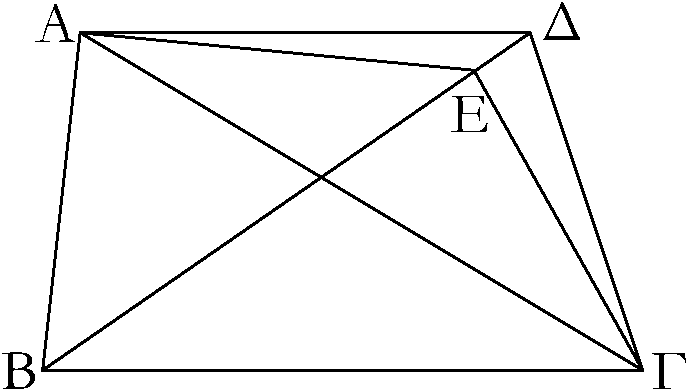
\includegraphics[width=0.8\textwidth]{Book01/fig39g.pdf}}

\gr{Τὰ   ἄρα ἴσα τρίγωνα τὰ ἐπὶ τῆς αὐτῆς βάσεως ὅντα καὶ ἐπὶ τὰ αὐτὰ μέρη καὶ ἐν ταῖς αὐταῖς παραλλήλοις ἐστίν; 
ὅπερ ἔδει δεῖχαι.}}

\ParallelRText{
\begin{center}
{\large Proposition 39}
\end{center}

Equal triangles which are on the same base, and on the same side, are
also between the same parallels.

Let $ABC$ and $DBC$ be equal triangles which are on the same base $BC$,
and on the same side (of it). I say that they are also between the same parallels.

For let $AD$ be joined. I say that $AD$ and $BC$ are parallel.

For, if not, let $AE$ be drawn through point A parallel to the straight-line $BC$ [Prop.~1.31], and let $EC$ be joined. Thus, triangle $ABC$ is equal
to triangle $EBC$. For it is on the same base as it, $BC$, and between the
same parallels [Prop.~1.37]. But $ABC$ is equal to $DBC$. Thus, $DBC$ is
also equal to $EBC$, the greater to the lesser. The very thing is impossible.
Thus, $AE$ is not parallel to $BC$. Similarly, we can show that neither (is)
any other (straight-line) than $AD$. Thus, $AD$ is parallel to $BC$.

% Removed epsf size command
\centerline{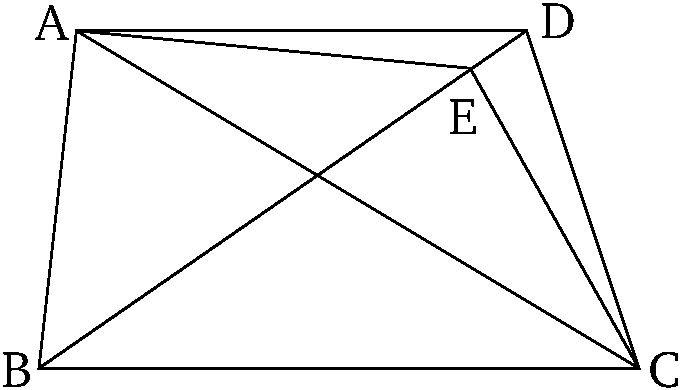
\includegraphics[width=0.8\textwidth]{Book01/fig39e.pdf}}

Thus, equal triangles which are on the same base, and on the same side, are
also between the same parallels. (Which is) the very thing it was required to show.}
\end{Parallel}

%%%%%%
% Prop 1.40
%%%%%%
\pdfbookmark[1]{Proposition 1.40}{pdf1.40}
\begin{Parallel}{}{} 
\ParallelLText{
\begin{center}
{\large\ggn{40}.}
\end{center}\vspace*{-7pt}

\gr{Τὰ  ἴσα τρίγωνα τὰ ἐπὶ ὸίσων βάσεων ὅντα καὶ ἐπὶ τὰ αὐτὰ μέρη καὶ ἐν ταῖς αὐταῖς παραλλήλοις ἐστίν.}

\gr{Ἔστω ἴσα τρίγωνα τὰ ΑΒΓ, ΓΔΕ ἐπὶ ὸίσων βάσεων τῶν ΒΓ, ΓΕ καὶ ἐπὶ τὰ αὐτὰ μέρη. λέγω, ὅτι καὶ ἐν ταῖς αὐταῖς παραλλήλοις ἐστίν.}

% Removed epsf size command
\centerline{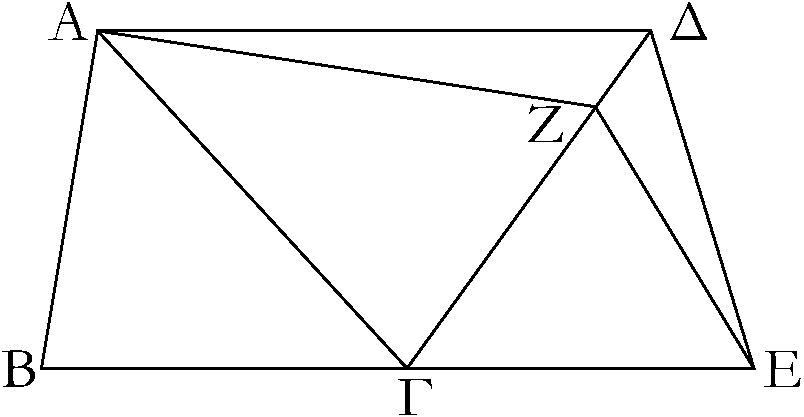
\includegraphics[width=0.8\textwidth]{Book01/fig40g.pdf}}

\gr{Ἐπεζεύθθω γὰρ ἡ ΑΔ; λέγω, ὅτι παράλληλόξ ἐστιν
ἡ ΑΔ τῇ ΒΕ.}

\gr{Εἰ γὰρ μή,  ἢθθω διὰ τοῦ Α τῇ ΒΕ παράλληλος ἡ ΑΖ, καὶ ἐπεζεύθθω ἡ ΖΕ.  ἴσον ἄρα ἐστὶ τὸ ΑΒΓ τρίγωνον τῷ ΖΓΕ τριγώνῳ; ἐπί τε
γὰρὸίσων βάσεών εἰσι τῶν ΒΓ, ΓΕ καὶ ἐν ταῖς αὐταῖς παραλλήλοις ταῖς ΒΕ, ΑΖ. ἀλλὰ τὸ ΑΒΓ τρίγωνον ἴσον ἐστὶ τῷ
ΔΓΕ  [τριγώνῳ]; καὶ τὸ ΔΓΕ ἄρα [τρίγωνον]  ἴσον ἐστὶ τῷ ΖΓΕ τριγώνῳ τὸ μεῖζον τῷ ἐλάσσονι; ὅπερ ἐστὶν ἀδύνατον; οὐκ ἄρα παράλληλος ἡ ΑΖ τῇ ΒΕ. ὁμοίως δὴ δείχομεν, ὅτι οὐδὸ ὸάλλη τις πλὴν τῆς ΑΔ; ἡ ΑΔ ἄρα τῇ ΒΕ ἐστι παράλληλος.}

\gr{Τὰ  ἄρα ἴσα τρίγωνα τὰ ἐπὶ ὸίσων βάσεων ὅντα καὶ ἐπὶ τὰ αὐτὰ μέρη καὶ ἐν ταῖς αὐταῖς παραλλήλοις ἐστίν;
ὅπερ ἔδει δεῖχαι.
}}

\ParallelRText{
\begin{center}
{\large Proposition 40$^\dag$}
\end{center}

Equal triangles which are on equal bases, and on the same side, are also
between the same parallels.

Let $ABC$ and $CDE$ be equal triangles on the equal bases $BC$ and $CE$ (respectively), and on the same side (of $BE$). I say that they are also between
the same parallels.

% Removed epsf size command
\centerline{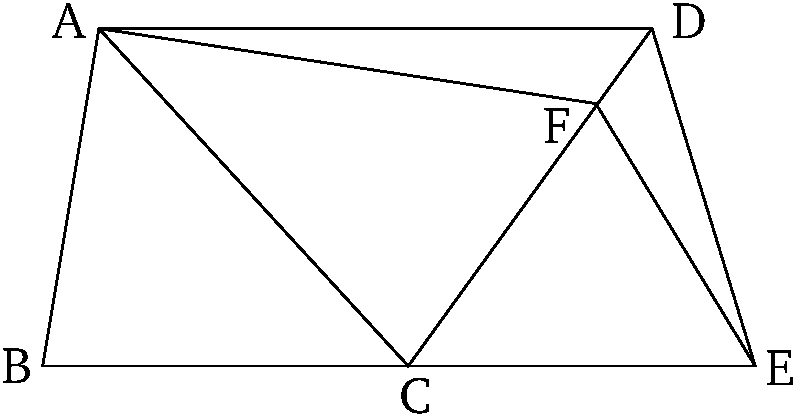
\includegraphics[width=0.8\textwidth]{Book01/fig40e.pdf}}

For let $AD$ be joined. I say that $AD$ is parallel to $BE$.

For if not, let $AF$ be drawn through $A$ parallel to $BE$ [Prop.~1.31],
and let $FE$ be joined. Thus, triangle $ABC$ is equal to triangle
$FCE$. For they are on equal bases, $BC$ and $CE$, and between the same
parallels, $BE$ and $AF$ [Prop.~1.38]. But, triangle $ABC$ is equal to [triangle] $DCE$.
Thus, [triangle] $DCE$ is also equal to triangle $FCE$, the greater to the
lesser. The very thing is impossible. 
Thus, $AF$ is not parallel to $BE$. Similarly, we can show that neither (is)
any other (straight-line) than $AD$. Thus, $AD$ is parallel to $BE$.

Thus, equal triangles which are on equal bases, and on the same side, are also
between the same parallels. (Which is) the very thing it was required to show.}
\end{Parallel}
{\footnotesize \noindent$^\dag$ This whole proposition is regarded by
Heiberg as a relatively early interpolation to the original text.\\}

%%%%%%
% Prop 1.41
%%%%%%
\pdfbookmark[1]{Proposition 1.41}{pdf1.41}
\begin{Parallel}{}{} 
\ParallelLText{
\begin{center}
{\large \ggn{41}.}
\end{center}\vspace*{-7pt}

\gr{Ἐὰν παραλληλόγραμμον τριγώνῳ βάσιν τεὸέθῃ τὴν αὐτὴν καὶ ἐν ταῖς αὐταῖς παραλλήλοιςὸῆ|, διπλάσιόν ἐστί τὸ παραλληλόγραμμον τοῦ
τριγώνου.}

\gr{Παραλληλόγραμμον γὰρ τὸ ΑΒΓΔ τριγώνῳ τῷ ΕΒΓ βάσιν τε ἐθέτω τὴν αὐτὴν τὴν ΒΓ καὶ ἐν ταῖς αὐταῖς παραλλήλοιςὸέστω ταῖς ΒΓ, ΑΕ; λέγω, ὅτι διπλάσιόν ἐστι τὸ ΑΒΓΔ παραλληλόγραμμον τοῦ ΒΕΓ τριγώνου.}

% Removed epsf size command
\centerline{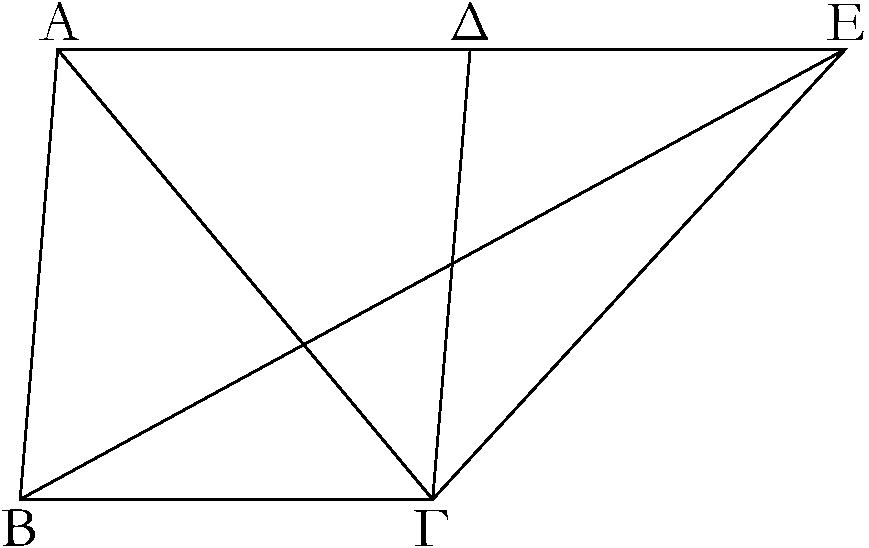
\includegraphics[width=0.8\textwidth]{Book01/fig41g.pdf}}

\gr{Ἐπεζεύθθω γὰρ ἡ ΑΓ.  ἴσον δή ἐστι τὸ ΑΒΓ τρίγωνον τῷ ΕΒΓ τριγώνῳ; ἐπί τε γὰρ τῆς αὐτῆς βάσεώξ ἐστιν αὐτῷ τῆς ΒΓ καὶ ἐν ταῖς αὐταῖς παραλλήλοις ταῖς ΒΓ, ΑΕ. ἀλλὰ τὸ ΑΒΓΔ παραλληλόγραμμον διπλάσιόν ἐστι τοῦ ΑΒΓ τριγώνου; ἡ γὰρ ΑΓ διάμετρος αὐτὸ δίθα τέμνει; ὁώστε τὸ ΑΒΓΔ παραλληλόγραμμον καὶ τοῦ ΕΒΓ τριγώνου ἐστὶ διπλάσιον.}

\gr{Ἐὰν ἄρα παραλληλόγραμμον τριγώνῳ βάσιν τεὸέθῃ τὴν αὐτὴν καὶ 
ἐν ταῖς αὐταῖς παραλλήλοιςὸῆ|, διπλάσιόν ἐστί τὸ παραλληλόγραμμον τοῦ
τριγώνου; ὅπερ ἔδει δεῖχαι.}}

\ParallelRText{
\begin{center}
{\large Proposition 41}
\end{center}

If a parallelogram has the same base as a triangle, and is between
the same parallels, (then) the parallelogram is double (the area) of the triangle.

For let parallelogram $ABCD$ have the same base $BC$ as triangle $EBC$,
and let it be between the same parallels, $BC$ and $AE$. I say that 
parallelogram $ABCD$ is double (the area) of triangle $BEC$.

% Removed epsf size command
\centerline{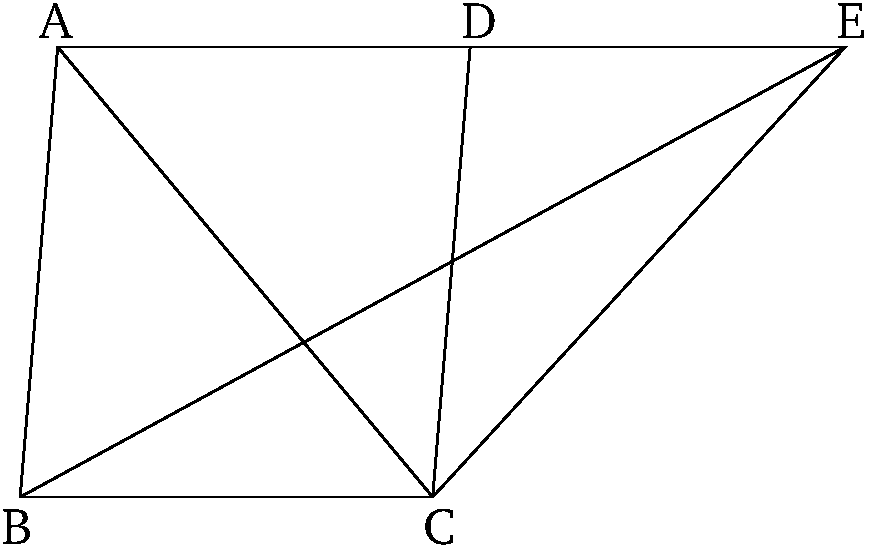
\includegraphics[width=0.8\textwidth]{Book01/fig41e.pdf}}

For let $AC$ be joined. So triangle $ABC$ is equal to triangle
$EBC$. For it is on the same base, $BC$,  (as $EBC$), and between the same
parallels, $BC$ and $AE$ [Prop.~1.37]. But, parallelogram $ABCD$
is double (the area) of triangle $ABC$. For the diagonal $AC$ cuts
the former in half [Prop.~1.34]. So parallelogram $ABCD$ is also
double (the area) of triangle $EBC$.

Thus, if a parallelogram has the same base as a triangle, and is between
the same parallels, (then) the parallelogram is double (the area) of the triangle.
(Which is) the very thing it was required to show.}
\end{Parallel}

%%%%%%
% Prop 1.42
%%%%%%
\pdfbookmark[1]{Proposition 1.42}{pdf1.42}
\begin{Parallel}{}{} 
\ParallelLText{
\begin{center}
{\large \ggn{42}.}
\end{center}\vspace*{-7pt}

\gr{Τῶ| δοθέντι τριγώνῳ  ἴσον παραλληλόγραμμον συστήσασθαι 
 ἐν τῇ δοθείσῃ γωνίᾳ εὐθυγράμμῳ.}
 
\gr{Ἔστω τὸ μὲν δοθὲν τρίγωνον τὸ ΑΒΓ, ἡ δὲ δοθεῖσα γωνία εὐθύγραμμος ἡ Δ; δεῖ δὴ τῷ ΑΒΓ τριγώνῳ  ἴσον παραλληλόγραμμον συστήσασθαι ἐν τῇ Δ γωνίᾳ εὐθυγράμμῳ.}

\gr{Τετμήσθω ἡ ΒΓ δίθα κατὰ τὸ Ε, καὶ ἐπεζεύθθω ἡ ΑΕ, καὶ συνεστάτω πρὸς τῇ ΕΓ εὐθείᾳ καὶ τῷ πρὸς αὐτῇ σημείῳ τῷ Ε τῇ Δ γωνίᾳ ὸίση ἡ ὑπὸ ΓΕΖ, καὶ διὰ μὲν τοῦ Α τῇ ΕΓ παράλληλος ἢθθω ἡ ΑΗ, διὰ δὲ τοῦ Γ τῇ ΕΖ παράλληλος ἢθθω ἡ ΓΗ; παραλληλόγραμμον ἄρα ἐστὶ τὸ ΖΕΓΗ. καὶ ἐπεὶ ὸίση ἐστὶν ἡ ΒΕ τῇ ΕΓ,  ἴσον ἐστὶ καὶ τὸ ΑΒΕ τρίγωνον τῷ ΑΕΓ τριγώνῳ; ἐπί τε γὰρὸίσων βάσεών εἰσι τῶν ΒΕ, ΕΓ καὶ ἐν ταῖς αὐταῖς παραλλήλοις ταῖς ΒΓ, ΑΗ; διπλάσιον ἄρα ἐστὶ τὸ ΑΒΓ τρίγωνον τοῦ ΑΕΓ τριγώνου. ὸέστι δὲ καὶ τὸ ΖΕΓΗ
παραλληλόγραμμον διπλάσιον τοῦ ΑΕΓ  τριγώνου; βάσιν τε γὰρ αὐτῷ τὴν αὐτὴν ἔχει καὶ ἐν ταῖς αὐταῖς ἐστιν αὐτῷ παραλλήλοις;  ἴσον ἄρα ἐστὶ τὸ ΖΕΓΗ παραλληλόγραμμον τῷ ΑΒΓ τριγώνῳ. καὶ  ἔχει τὴν ὑπὸ ΓΕΖ γωνίαν ἴσην τῇ δοθείσῃ τῇ Δ.}

% Removed epsf size command
\centerline{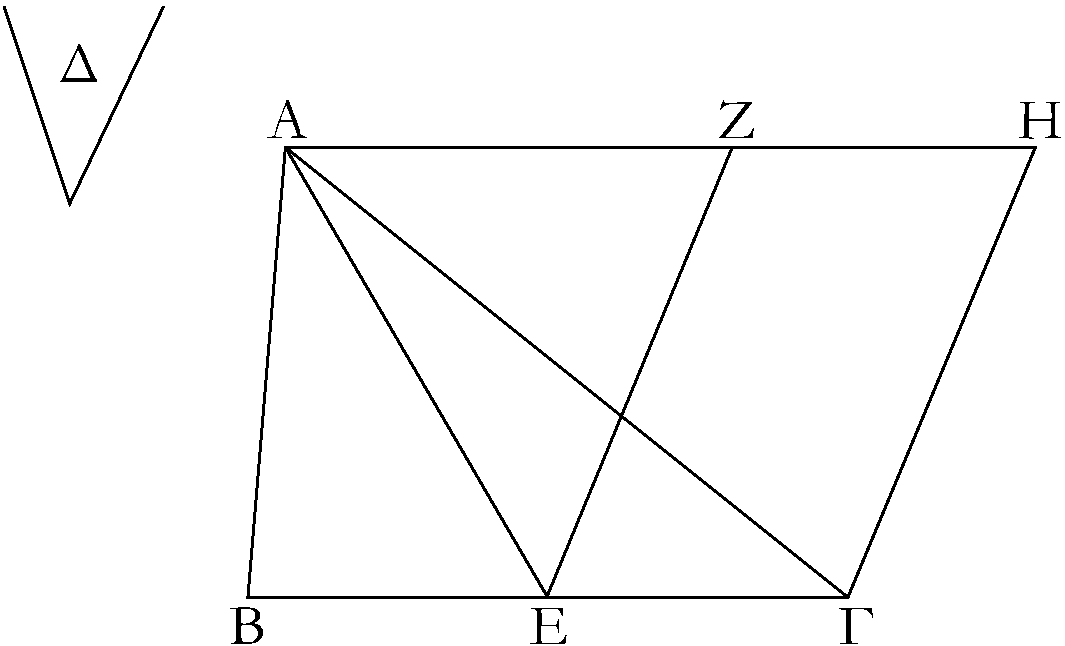
\includegraphics[width=0.8\textwidth]{Book01/fig42g.pdf}}

\gr{Τῶ|  ἄρα δοθέντι τριγώνῳ τῷ ΑΒΓ ἴσον παραλληλόγραμμον συνέσταται τὸ ΖΕΓΗ ἐν γωνίᾳ τῇ ὑπὸ ΓΕΖ, ἥτις ἐστὶνὸίση τῇ Δ;
ὅπερ ἔδει ποιῆσαι.}}

\ParallelRText{
\begin{center}
{\large Proposition 42}
\end{center}

To construct a parallelogram equal to a given triangle in a given
rectilinear angle.

Let $ABC$ be the given triangle, and $D$ the given rectilinear angle. So
it is required to construct a parallelogram equal to triangle $ABC$
in the rectilinear angle $D$.

Let $BC$ be cut in half at $E$ [Prop.~1.10], and let $AE$ be joined. And let (angle) $CEF$, equal to angle $D$,  be constructed
at the point $E$ on the straight-line $EC$ [Prop.~1.23]. And let $AG$ be drawn through $A$
parallel to $EC$ [Prop.~1.31], and let $CG$ be drawn through $C$ parallel
to $EF$ [Prop.~1.31]. Thus, $FECG$ is a parallelogram. And since $BE$ is
equal to $EC$, triangle $ABE$ is also equal to triangle $AEC$. For they are
on the equal bases, $BE$ and $EC$, and between the same parallels, $BC$ and $AG$ [Prop.~1.38]. Thus, triangle $ABC$ is double (the area) of triangle $AEC$. And
parallelogram $FECG$ is also double (the area) of triangle $AEC$. For it has the same base (as $AEC$), and is between the same parallels  (as $AEC$) [Prop.~1.41].
Thus, parallelogram $FECG$ is equal to triangle $ABC$.  ($FECG$) also has
the angle $CEF$ equal to the given (angle) $D$.

% Removed epsf size command
\centerline{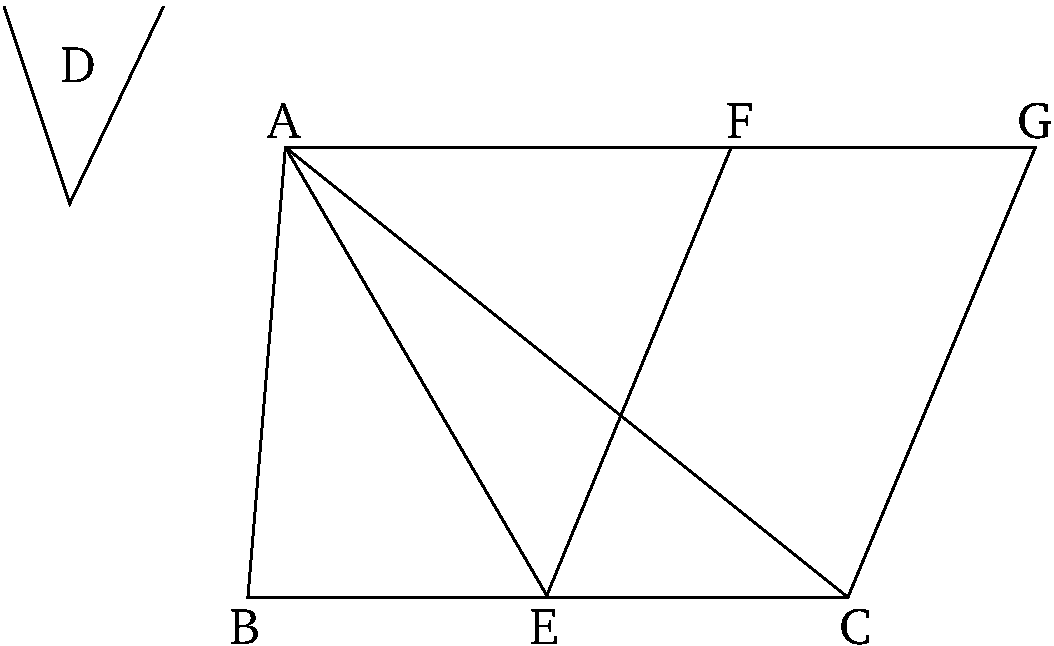
\includegraphics[width=0.8\textwidth]{Book01/fig42e.pdf}}

Thus, parallelogram $FECG$,  equal to the given
triangle $ABC$, has been constructed in the angle $CEF$, which is equal to $D$. (Which is) the
very thing it was required to do.}
\end{Parallel}

%%%%%%
% Prop 1.43
%%%%%%
\pdfbookmark[1]{Proposition 1.43}{pdf1.43}
\begin{Parallel}{}{} 
\ParallelLText{
\begin{center}
{\large \ggn{43}.}
\end{center}\vspace*{-7pt}

\gr{Παντὸξ παραλληλογράμμου τῶν περὶ τὴν διάμετρον παραλληλογράμμων τὰ παραπληρώματα ἴσα ἀλλήλοις ἐστίν.}

\gr{Ἔστω παραλληλόγραμμον τὸ ΑΒΓΔ, διάμετρος δὲ αὐτοῦ ἡ ΑΓ, περὶ
δὲ τὴν ΑΓ παραλληλόγραμμα μὲνὸέστω τὰ ΕΘ, ΖΗ, τὰ δὲ λεγόμενα παραπληρώματα τὰ ΒΚ, ΚΔ; λέγω, ὅτι ἴσον ἐστὶ τὸ ΒΚ παραπλήρωμα τῷ ΚΔ
παραπληρώματι.}

% Removed epsf size command
\centerline{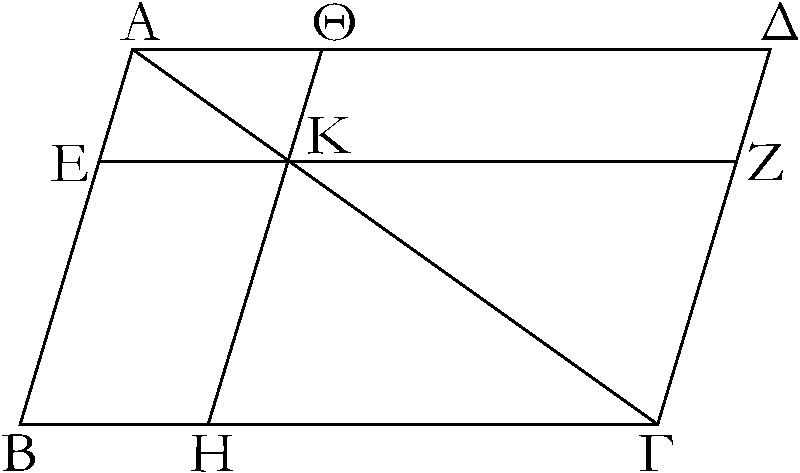
\includegraphics[width=0.8\textwidth]{Book01/fig43g.pdf}}

\gr{Ἐπεὶ γὰρ παραλληλόγραμμόν ἐστι τὸ ΑΒΓΔ, διάμετρος δὲ αὐτοῦ ἡ
ΑΓ,  ἴσον ἐστὶ τὸ ΑΒΓ τρίγωνον τῷ ΑΓΔ τριγώνῳ. πάλιν, ἐπεὶ παραλληλόγραμμόν ἐστι τὸ ΕΘ, διάμετρος δὲ αὐτοῦ ἐστιν ἡ ΑΚ,
 ἴσον ἐστὶ τὸ ΑΕΚ τρίγωνον τῷ ΑΘΚ τριγώνῳ. διὰ τὰ αὐτὰ δὴ καὶ τὸ ΚΖΓ τρίγωνον τῷ ΚΗΓ ἐστιν ἴσον. ἐπεὶ οὸῦν τὸ μὲν ΑΕΚ τρίγωνον τῷ ΑΘΚ τριγώνῳ ἐστὶν ἴσον, τὸ δὲ ΚΖΓ τῷ ΚΗΓ, τὸ 
ΑΕΚ τρίγωνον μετὰ τοῦ ΚΗΓ ἴσον ἐστὶ
τῷ ΑΘΚ  τριγώνῳ μετὰ τοῦ ΚΖΓ; ὸέστι δὲ καὶ ὅλον τὸ ΑΒΓ τρίγωνον ὅλῳ τῷ ΑΔΓ ἴσον; λοιπὸν ἄρα τὸ ΒΚ παραπλήρωμα λοιπῶ| τῷ ΚΔ παραπληρώματί ἐστιν ἴσον.}

\gr{Παντὸξ ἄρα παραλληλογράμμου θωρίου τῶν περὶ τὴν διάμετρον παραλληλογράμμων τὰ παραπληρώματα ἴσα ἀλλήλοις ἐστίν; ὅπερ ἔδει δεῖχαι.}}

\ParallelRText{
\begin{center}
{\large Proposition 43}
\end{center}

For any parallelogram, the complements of the parallelograms about the diagonal are equal to one another.

Let $ABCD$ be a parallelogram, and $AC$ its diagonal. And let $EH$ and $FG$
be the parallelograms about  $AC$, and $BK$ and $KD$ the so-called complements
(about $AC$).
I say that the complement $BK$ is equal to the complement $KD$.

% Removed epsf size command
\centerline{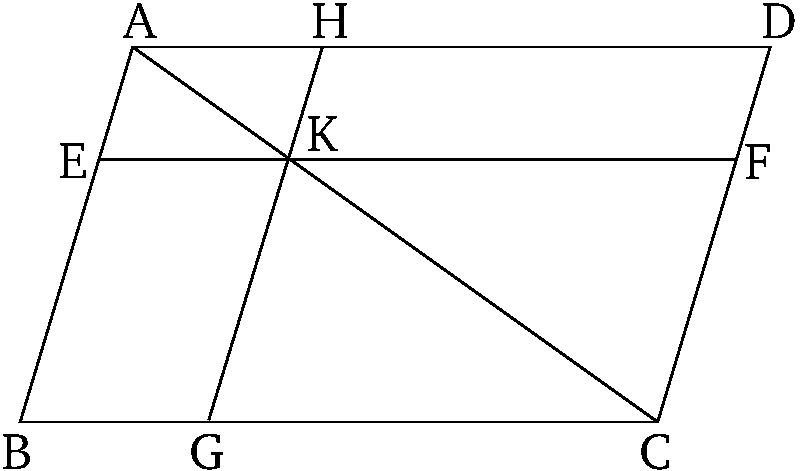
\includegraphics[width=0.8\textwidth]{Book01/fig43e.pdf}}

For since $ABCD$ is a parallelogram, and $AC$ its diagonal,  triangle
$ABC$ is equal to triangle $ACD$ [Prop.~1.34]. Again, since $EH$ is
a parallelogram, and $AK$ is its diagonal, triangle $AEK$ is equal to
triangle $AHK$ [Prop.~1.34]. So, for the same (reasons), triangle
$KFC$ is also equal to (triangle) $KGC$. Therefore, since triangle $AEK$ is
equal to triangle $AHK$, and $KFC$ to $KGC$, triangle $AEK$ plus $KGC$ is
equal to triangle $AHK$ plus $KFC$. And the whole triangle $ABC$ is
also equal to the whole (triangle) $ADC$. Thus, the remaining complement
$BK$ is equal to the remaining complement $KD$.

Thus, for any parallelogramic figure, the complements of the
parallelograms about the diagonal are equal to one another.
(Which is) the very thing it was required to show.}
\end{Parallel}

%%%%%%
% Prop 1.44
%%%%%%
\pdfbookmark[1]{Proposition 1.44}{pdf1.44}
\begin{Parallel}{}{} 
\ParallelLText{
\begin{center}
{\large \ggn{44}.}
\end{center}\vspace*{-7pt}

\gr{Παρὰ τὴν δοθεῖσαν εὐθεῖαν τῷ δοθέντι  τριγώνῳ  ἴσον παραλληλόγραμμον παραβαλεῖν ἐν  τῇ δοθείσῃ γωνίᾳ εὐθυγράμμῳ.}

\gr{Ἔστω ἡ μὲν δοθεῖσα εὐθεῖα ἡ ΑΒ, τὸ δὲ δοθὲν τρίγωνον τὸ Γ, ἡ δὲ δοθεῖσα γωνία εὐθύγραμμος ἡ Δ; δεῖ δὴ παρὰ τὴν δοθεῖσαν εὐθεῖαν τὴν ΑΒ τῷ δοθέντι τριγώνῳ τῷ Γ ἴσον παραλληλόγραμμον
παραβαλεῖν ἐνὸίσῃ τῇ Δ γωνίᾳ.}

% Removed epsf size command
\centerline{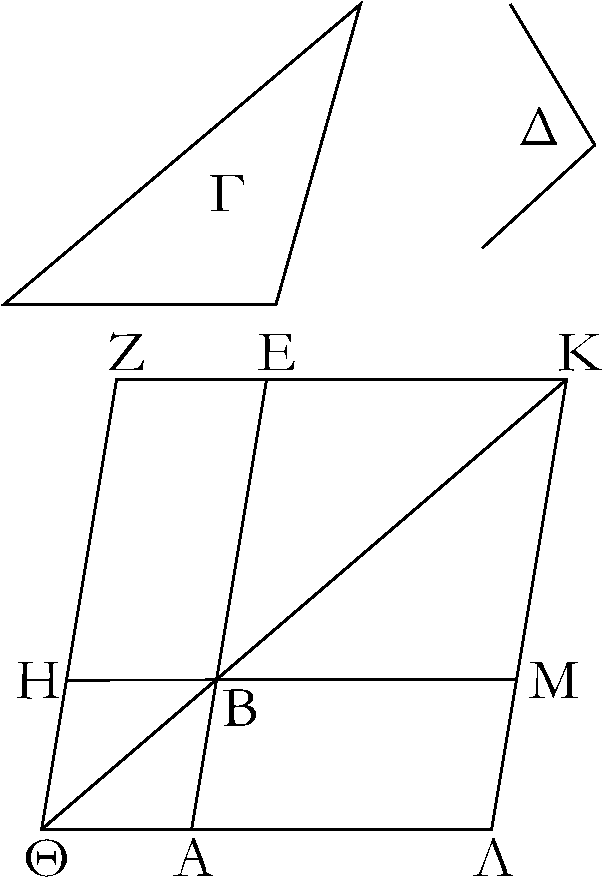
\includegraphics[width=0.8\textwidth]{Book01/fig44g.pdf}}

\gr{Συνεστάτω τῷ Γ τριγώνῳ  ἴσον παραλληλόγραμμον τὸ ΒΕΖΗ ἐν γωνίᾳ τῇ ὑπὸ ΕΒΗ, ἥ ἐστινὸίση τῇ Δ; καὶ κείσθω ὁώστε ἐπ' εὐθείας εὸῖναι τὴν ΒΕ τῇ ΑΒ, καὶ διήθθω ἡ ΖΗ ἐπὶ τὸ Θ, καὶ διὰ τοῦ 
Α ὁποτέρᾳ τῶν ΒΗ, ΕΖ παράλληλος ἢθθω ἡ ΑΘ, καὶ ἐπεζεύθθω ἡ ΘΒ. καὶ ἐπεὶ εἰξ παραλλήλους τὰξ ΑΘ, ΕΖ εὐθεῖα ἐνέπεσεν ἡ ΘΖ, αἱ
 ἄρα ὑπὸ  ΑΘΖ, ΘΖΕ γωνίαι δυσὶν ὀρθαῖξ εἰσιν ἴσαι. αἱ  ἄρα ὑπὸ ΒΘΗ, ΗΖΕ δύο ὀρθῶν ἐλάσσονέξ εἰσιν; αἱ δὲ ἀπὸ ἐλασσόνωνὸὴ δύο ὀρθῶν εἰξ ἄπειρον ἐκβαλλόμεναι συμπίπτουσιν; αἱ ΘΒ, ΖΕ ἄρα ἐκβαλλόμεναι συμπεσοῦνται. ἐκβεβλήσθωσαν καὶ συμπιπτέτωσαν κατὰ τὸ Κ, καὶ διὰ τοῦ Κ σημείου ὁποτέρᾳ τῶν ΕΑ, ΖΘ παράλληλος ἢθθω ἡ
ΚΛ, καὶ ἐκβεβλήσθωσαν αἱ ΘΑ, ΗΒ ἐπὶ τὰ Λ, Μ σημεῖα. παραλληλόγραμμον ἄρα ἐστὶ 
τὸ ΘΛΚΖ, διάμετρος δὲ αὐτοῦ ἡ ΘΚ, περὶ δὲ τὴν ΘΚ παραλληλόγραμμα μὲν τὰ ΑΗ, ΜΕ, τὰ δὲ λεγόμενα παραπληρώματα τὰ ΛΒ, ΒΖ;  ἴσον ἄρα ἐστὶ τὸ ΛΒ τῷ ΒΖ. ἀλλὰ τὸ ΒΖ τῷ Γ τριγώνῳ ἐστὶν ἴσον; καὶ τὸ ΛΒ ἄρα τῷ Γ ἐστιν ἴσον. καὶ ἐπεὶ ὸίση ἐστὶν ἡ ὑπὸ ΗΒΕ γωνία τῇ ὑπὸ ΑΒΜ, ἀλλὰ ἡ ὑπὸ ΗΒΕ τῇ Δ ἐστινὸίση, καὶ ἡ ὑπὸ ΑΒΜ ἄρα τῇ Δ γωνίᾳ ἐστὶνὸίση.}

\gr{Παρὰ τὴν δοθεῖσαν ἄρα εὐθεῖαν τὴν ΑΒ τῷ δοθέντι τριγώνῳ τῷ
Γ ἴσον παραλληλόγραμμον παραβέβληται τὸ ΛΒ ἐν γωνίᾳ τῇ ὑπὸ
ΑΒΜ,  ἥ ἐστινὸίση τῇ Δ; ὅπερ ἔδει ποιῆσαι.}}

\ParallelRText{
\begin{center}
{\large Proposition 44}
\end{center}

To apply a parallelogram equal to a given triangle to a given straight-line
in a given rectilinear angle.

Let $AB$ be the given straight-line,  $C$ the given triangle, and $D$ the
given rectilinear angle. So it is required to apply a parallelogram
equal to the given triangle $C$ to the given straight-line $AB$ in an angle equal to (angle) $D$.

% Removed epsf size command
\centerline{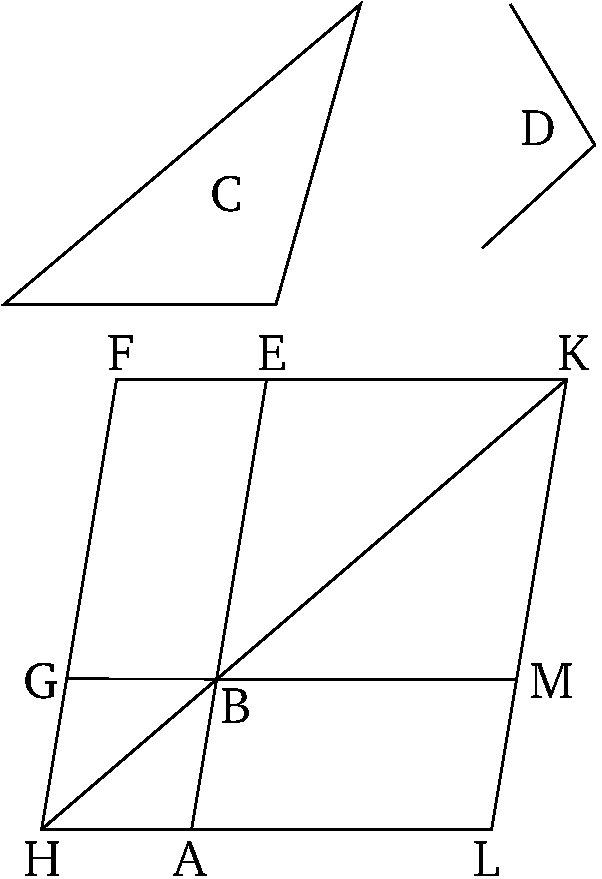
\includegraphics[width=0.8\textwidth]{Book01/fig44e.pdf}}

Let the parallelogram $BEFG$, equal to the triangle $C$, be
constructed in the angle $EBG$, which is equal to $D$ [Prop.~1.42].
And let it be placed so that $BE$ is straight-on to $AB$.$^\dag$  And
let $FG$ be drawn through to $H$, and let $AH$ be
drawn through $A$ parallel to either of $BG$ or $EF$ [Prop.~1.31], and
let $HB$ be joined. And since the straight-line $HF$ falls across the
parallels $AH$ and $EF$, the (sum of the) angles $AHF$ and $HFE$ is thus equal to
two right-angles [Prop.~1.29]. Thus, (the sum of) $BHG$ and $GFE$ is less than two
right-angles.
And (straight-lines) produced to
infinity from (internal angles whose sum is) less than two right-angles meet together [Post.~5].
Thus, being produced, $HB$ and $FE$ will meet together. Let them 
be produced, and let them meet together at $K$. And let $KL$ be
drawn through point $K$ parallel to either of $EA$ or $FH$ [Prop.~1.31]. And
let $HA$ and $GB$ be produced to points $L$ and $M$ (respectively). Thus, $HLKF$ is a parallelogram, and $HK$ its diagonal. And $AG$ and $ME$ (are) parallelograms, and $LB$ and $BF$ the so-called complements, about $HK$. Thus, $LB$ is
equal to $BF$ [Prop.~1.43]. But, $BF$ is equal to triangle $C$. Thus, $LB$ is also
equal to $C$. Also, since angle $GBE$ is equal to $ABM$ [Prop.~1.15], but
$GBE$ is equal to $D$, $ABM$ is thus also equal to angle $D$.

Thus, the parallelogram $LB$, equal to the
given triangle $C$, has been applied to the given straight-line
$AB$ in the angle $ABM$, which is equal to $D$. (Which is) the very thing it was required to do.}
\end{Parallel}
{\footnotesize \noindent$^\dag$ This can be achieved using Props.~1.3, 1.23, and 1.31.}

%%%%%%
% Prop 1.45
%%%%%%
\pdfbookmark[1]{Proposition 1.45}{pdf1.45}
\begin{Parallel}{}{} 
\ParallelLText{
\begin{center}
{\large \ggn{45}.}
\end{center}
\vspace*{-7pt}

\gr{Τῶ| δοθέντι εὐθυγράμμῳ  ἴσον παραλληλόγραμμον συστήσασθαι ἐν τῇ
δοθείσῃ γωνίᾳ εὐθυγράμμῳ.}

\gr{Ἔστω τὸ μὲν δοθὲν εὐθύγραμμον τὸ ΑΒΓΔ, ἡ δὲ δοθεῖσα γωνία εὐθύγραμμος ἡ Ε; δεῖ δὴ τῷ ΑΒΓΔ εὐθυγράμμῳ  ἴσον παραλληλόγραμμον συστήσασθαι ἐν τῇ δοθείσῃ γωνίᾳ τῇ Ε.}

% Removed epsf size command
\centerline{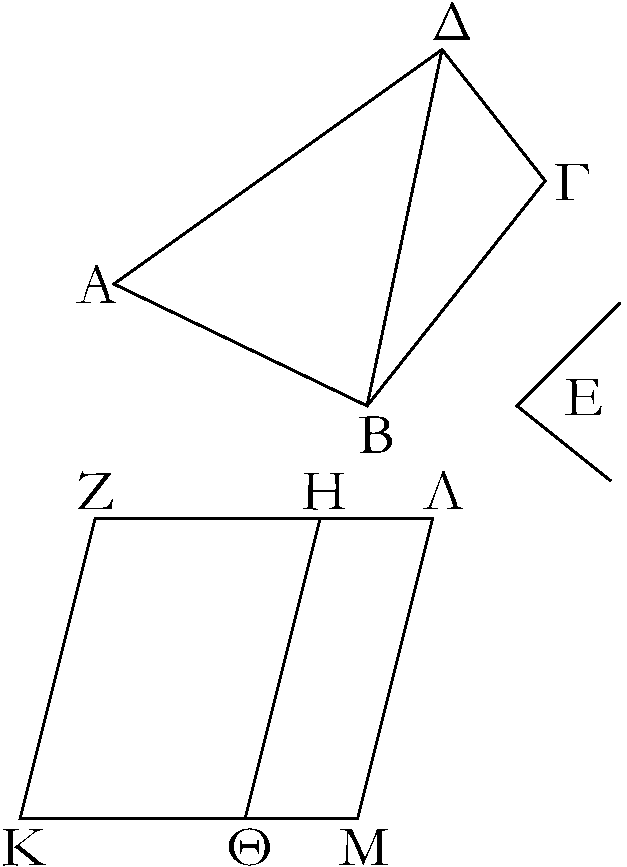
\includegraphics[width=0.8\textwidth]{Book01/fig45g.pdf}}

\gr{Ἐπεζεύθθω ἡ ΔΒ, καὶ συνεστάτω τῷ ΑΒΔ τριγώνῳ  ἴσον παραλληλόγραμμον τὸ ΖΘ ἐν τῇ ὑπὸ ΘΚΖ γωνίᾳ, ἥ ἐστινὸίση τῇ Ε;
καὶ παραβεβλήσθω παρὰ τὴν ΗΘ εὐθεῖαν τῷ ΔΒΓ τριγώνῳ  ἴσον παραλληλόγραμμον τὸ ΗΜ ἐν τῇ ὑπὸ ΗΘΜ γωνίᾳ, ἥ ἐστινὸίση τῇ Ε. καὶ ἐπεὶ ἡ Ε γωνία ἑκατέρᾳ τῶν ὑπὸ ΘΚΖ, ΗΘΜ ἐστινὸίση, καὶ ἡ ὑπὸ ΘΚΖ ἄρα τῇ ὑπὸ ΗΘΜ ἐστινὸίση. κοινὴ προσκείσθω ἡ ὑπὸ ΚΘΗ; αἱ  ἄρα ὑπὸ ΖΚΘ, ΚΘΗ ταῖς ὑπὸ ΚΘΗ, ΗΘΜ ἴσαι εἰσίν.
ἀλλὸ αἱ ὑπὸ ΖΚΘ, ΚΘΗ
 δυσὶν ὀρθαῖξ ἴσαι εἰσίν; καὶ αἱ  ὑπὸ ΚΘΗ, ΗΘΜ ἄρα δύο ὀρθαῖξ ἴσαι εἰσίν.
  πρὸς δή τινι εὐθεῖᾳ τῇ ΗΘ καὶ τῷ πρὸς αὐτῇ σημείῳ τῷ Θ δύο εὐθεῖαι
 αἱ ΚΘ, ΘΜ 
 μὴ ἐπὶ τὰ αὐτὰ μέρη κείμεναι τὰξ ἐφεχῆς γωνίας δύο ὀρθαῖξ ἴσας ποιοῦσιν; ἐπ' εὐθείας ἄρα ἐστὶν ἡ ΚΘ
τῇ ΘΜ; καὶ ἐπεὶ εἰξ παραλλήλους τὰξ ΚΜ, ΖΗ εὐθεῖα ἐνέπεσεν ἡ ΘΗ, αἱ ἐναλλὰχ γωνίαι αἱ ὑπὸ ΜΘΗ, ΘΗΖ ἴσαι ἀλλήλαις εἰσίν. κοινὴ
προσκείσθω ἡ ὑπὸ ΘΗΛ; αἱ  ἄρα ὑπὸ ΜΘΗ, ΘΗΛ ταῖς ὑπὸ ΘΗΖ, ΘΗΛ ἴσαι εἰσιν. ἀλλὸ αἱ ὑπὸ ΜΘΗ, ΘΗΛ
δύο ὀρθαῖξ ἴσαι
εἰσίν; καὶ αἱ ὑπὸ ΘΗΖ, ΘΗΛ ἄρα δύο ὀρθαῖξ ἴσαι εἰσίν;
ἐπ' εὐθείας ἄρα ἐστὶν ἡ ΖΗ τῇ ΗΛ. καὶ ἐπεὶ ἡ ΖΚ τῇ ΘΗὸίση τε καὶ παράλληλόξ ἐστιν, ἀλλὰ καὶ ἡ ΘΗ τῇ ΜΛ, καὶ ἡ ΚΖ ἄρα τῇ ΜΛὸίση τε καὶ παράλληλόξ ἐστιν; καὶ ἐπιζευγνύουσιν αὐτὰξ εὐθεῖαι αἱ ΚΜ, ΖΛ; καὶ αἱ ΚΜ, ΖΛ ἄρα ἴσαι τε καὶ παράλληλοί εἰσιν; παραλληλόγραμμον ἄρα ἐστὶ τὸ ΚΖΛΜ. καὶ ἐπεὶ  ἴσον ἐστὶ τὸ μὲν
ΑΒΔ τρίγωνον τῷ ΖΘ παραλληλογράμμῳ, τὸ δὲ ΔΒΓ τῷ ΗΜ, ὅλον ἄρα τὸ ΑΒΓΔ εὐθύγραμμον ὅλῳ τῷ ΚΖΛΜ
παραλληλογράμμῳ ἐστὶν ἴσον.}

\gr{Τῶ|  ἄρα δοθέντι εὐθυγράμμῳ τῷ ΑΒΓΔ ἴσον παραλληλόγραμμον συνέσταται τὸ ΚΖΛΜ ἐν γωνίᾳ τῇ ὑπὸ ΖΚΜ, ἥ ἐστινὸίση τῇ
δοθείσῃ τῇ Ε; ὅπερ ἔδει ποιῆσαι.}}

\ParallelRText{
\begin{center}
{\large Proposition 45}
\end{center}

To construct a parallelogram equal to a given rectilinear figure in a given
rectilinear angle.

Let $ABCD$ be the given rectilinear figure,$^\dag$ and $E$ the given rectilinear angle.
So it is required to construct a parallelogram equal to the rectilinear figure
$ABCD$ in the given angle $E$.

% Removed epsf size command
\centerline{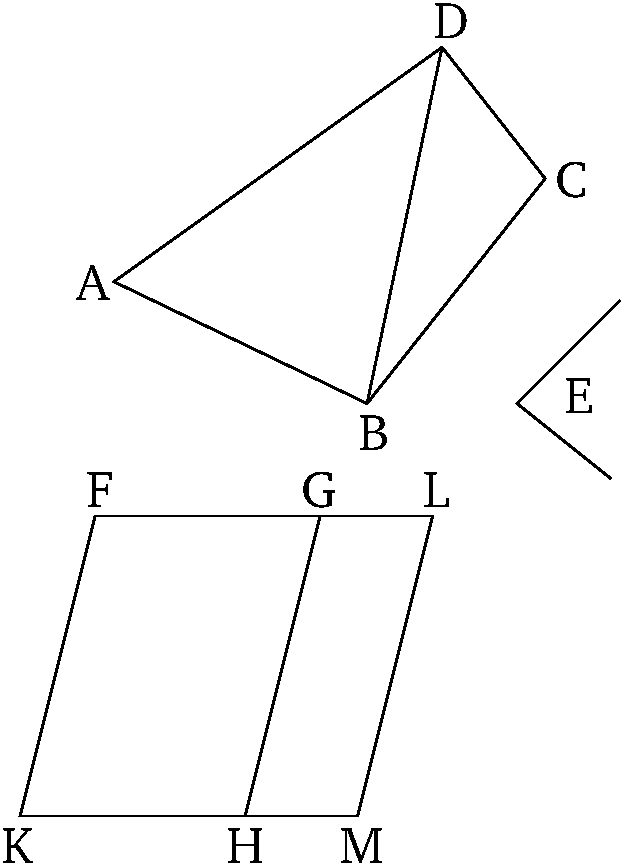
\includegraphics[width=0.8\textwidth]{Book01/fig45e.pdf}}

Let $DB$ be joined, and let the parallelogram $FH$, equal to
the triangle $ABD$, be
constructed in the angle $HKF$, which is equal to $E$ [Prop.~1.42].
And let the parallelogram $GM$, equal to the triangle $DBC$, be
applied to the straight-line $GH$ in the angle $GHM$,
which is equal to $E$ [Prop.~1.44]. And since angle $E$ is equal to each of
(angles) $HKF$ and $GHM$,  (angle) $HKF$ is thus also equal to $GHM$. 
Let $KHG$ be added to both. Thus, (the sum of) $FKH$ and $KHG$ is
equal to (the sum of) $KHG$ and $GHM$. But, (the sum of) $FKH$ and $KHG$ is equal to
two right-angles [Prop.~1.29]. Thus, (the sum of) $KHG$ and $GHM$ is also equal to
two right-angles. So two straight-lines, $KH$ and $HM$, not lying on the same side, make  adjacent angles with some straight-line $GH$, 
at the point $H$ on it, (whose sum is) equal to two right-angles.
Thus, $KH$ is straight-on to $HM$ [Prop.~1.14].
And since the straight-line $HG$ falls across the parallels $KM$ and $FG$, the alternate angles
$m\kern -.7pt hG$ and $HGF$ are equal to one another [Prop.~1.29]. Let $HGL$ have
been added to both. Thus, (the sum of) $m\kern -.7pt hG$ and $HGL$ is equal to 
(the sum of) $HGF$ and $HGL$.
But, (the sum of) $m\kern -.7pt hG$ and $HGL$ is equal to two right-angles [Prop.~1.29].
Thus, (the sum of) $HGF$ and $HGL$ is also equal to two right-angles.
Thus, $FG$ is straight-on to $GL$ [Prop.~1.14]. And since $FK$ is
equal and parallel to $HG$ [Prop.~1.34], but also $HG$ to $ML$ [Prop.~1.34],
$KF$ is thus also equal and parallel to $ML$ [Prop.~1.30]. And the straight-lines $KM$ and
$FL$ join them. Thus, $KM$ and $FL$ are equal and parallel as well [Prop.~1.33].
Thus, $KFLM$ is a parallelogram. And since triangle $ABD$ is equal to parallelogram $FH$, and $DBC$ to $GM$, the whole rectilinear figure
$ABCD$ is thus equal to the whole parallelogram $KFLM$.

Thus, the parallelogram $KFLM$, equal to the given
rectilinear figure $ABCD$, has been constructed in the angle
$FKM$, which is equal to the given (angle) $E$. (Which is) the very thing it was
required to do.}
\end{Parallel}
{\footnotesize \noindent$^\dag$ The proof is only given for a four-sided figure. However, the extension to many-sided figures is
trivial.}

%%%%%%
% Prop 1.46
%%%%%%
\pdfbookmark[1]{Proposition 1.46}{pdf1.46}
\begin{Parallel}{}{} 
\ParallelLText{
\begin{center}
{\large \ggn{46}.}
\end{center}\vspace*{-7pt}

\gr{Ἀπὸ τῆς δοθείσης εὐθείας τετράγωνον ἀναγράψαι.}

\gr{Ἔστω ἡ δοθεῖσα εὐθεῖα ἡ ΑΒ; δεῖ δὴ ἀπὸ τῆς ΑΒ εὐθείας τετράγωνον ἀναγράψαι.}

% Removed epsf size command
\centerline{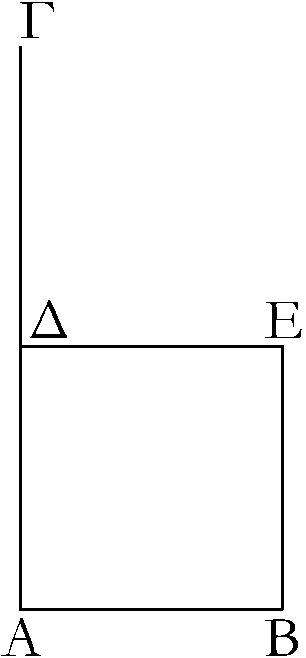
\includegraphics[width=0.8\textwidth]{Book01/fig46g.pdf}}

\gr{ὸ'Ηθθω τῇ ΑΒ εὐθείᾳ ἀπὸ τοῦ πρὸς αὐτῇ σημείου τοῦ Α πρὸς ὀρθὰξ ἡ ΑΓ, καὶ κείσθω τῇ ΑΒὸίση ἡ ΑΔ; καὶ διὰ μὲν τοῦ Δ σημείου τῇ ΑΒ παράλληλος ἢθθω ἡ ΔΕ, διὰ δὲ τοῦ Β σημείου τῇ ΑΔ παράλληλος ἢθθω ἡ ΒΕ. παραλληλόγραμμον ἄρα ἐστὶ τὸ ΑΔΕΒ; ὸίση ἄρα ἐστὶν ἡ μὲν ΑΒ τῇ ΔΕ, ἡ δὲ ΑΔ τῇ ΒΕ. ἀλλὰ ἡ ΑΒ τῇ ΑΔ ἐστινὸίση; αἱ τέσσαρες ἄρα αἱ ΒΑ, ΑΔ, ΔΕ, ΕΒ ἴσαι ἀλλήλαις εἰσίν;
ἰσόπλευρον ἄρα ἐστὶ τὸ ΑΔΕΒ παραλληλόγραμμον. λέγω δή, ὅτι καὶ ὀρθογώνιον. ἐπεὶ γὰρ εἰξ παραλλήλους τὰξ ΑΒ, ΔΕ εὐθεῖα ἐνέπεσεν ἡ ΑΔ, αἱ  ἄρα ὑπὸ ΒΑΔ, ΑΔΕ γωνίαι δύο ὀρθαῖξ ἴσαι εἰσίν.
ὀρθὴ δὲ ἡ ὑπὸ ΒΑΔ; ὀρθὴ  ἄρα καὶ ἡ ὑπὸ ΑΔΕ. τῶν δὲ παραλληλογράμμων θωρίων αἱ ἀπεναντίον πλευραί τε καὶ γωνίαι ἴσαι ἀλλήλαις εἰσίν; ὀρθὴ  ἄρα καὶ ἑκατέρα τῶν ἀπεναντίον τῶν ὑπὸ ΑΒΕ, ΒΕΔ γωνιῶν; ὀρθογώνιον ἄρα ἐστὶ τὸ ΑΔΕΒ. ἐδείθθη δὲ καὶ ἰσόπλευρον.}

\gr{Τετράγωνον ἄρα ἐστίν; καί ἐστιν ἀπὸ τῆς ΑΒ εὐθείας ἀναγεγραμμένον; ὅπερ ἔδει ποιῆσαι.}}

\ParallelRText{
\begin{center}
{\large Proposition 46}
\end{center}

To describe a square on a given straight-line.

Let $AB$ be the given straight-line. So it is required to describe a
square on the straight-line $AB$.

% Removed epsf size command
\centerline{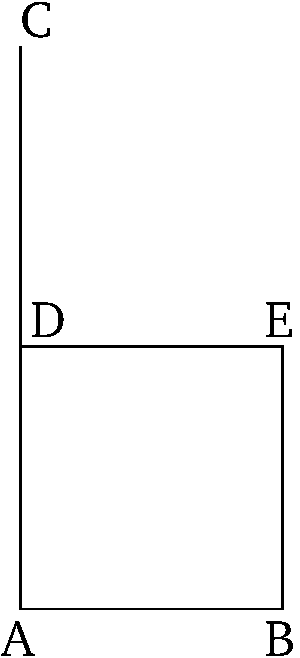
\includegraphics[width=0.8\textwidth]{Book01/fig46e.pdf}}

Let $AC$ be drawn at right-angles to the straight-line $AB$
from the point $A$ on it [Prop.~1.11], and let $AD$ be
made equal to $AB$ [Prop.~1.3]. And let $DE$ be drawn
through point $D$ parallel to $AB$ [Prop.~1.31], and let $BE$ be
drawn through point $B$ parallel to $AD$ [Prop.~1.31]. Thus,
$ADEB$ is a parallelogram. Therefore, $AB$ is equal to $DE$, and $AD$ to $BE$ [Prop.~1.34]. But, $AB$ is equal to $AD$. Thus, the four (sides) $BA$, $AD$, $DE$, and $EB$ are equal to one another. Thus, the parallelogram $ADEB$ is equilateral.
So I say that (it is) also right-angled. For since the straight-line $AD$ falls
across the parallels $AB$ and $DE$, the (sum of the) angles $BAD$ and $ADE$ is
equal to two right-angles [Prop.~1.29]. But $BAD$ (is a) right-angle. Thus,
$ADE$ (is) also a right-angle. And for parallelogramic figures, the opposite
sides and angles are equal to one another [Prop.~1.34]. Thus, each of the
opposite angles $ABE$ and $BED$ (are) also right-angles. Thus, $ADEB$ is
right-angled. And it was also shown (to be) equilateral.

Thus, ($ADEB$) is a square [Def.~1.22]. And it is described on the straight-line $AB$. (Which is) the very thing it was required to do.}
\end{Parallel}

%%%%%%
% Prop 1.47
%%%%%%
\pdfbookmark[1]{Proposition 1.47}{pdf1.47}
\begin{Parallel}{}{} 
\ParallelLText{
\begin{center}
{\large\ggn{47}.}
\end{center}\vspace*{-7pt}

\gr{Ἐν τοῖς ὀρθογωνίοις τριγώνοις τὸ ἀπὸ τῆς τὴν ὀρθὴν γωνίαν ὑποτεινούσης πλευρᾶξ τετράγωνον ἴσον ἐστὶ τοῖς ἀπὸ τῶν τὴν ὀρθὴν γωνίαν περιεθουσῶν πλευρῶν τετραγώνοις.}

\gr{Ἔστω τρίγωνον ὀρθογώνιον τὸ ΑΒΓ ὀρθὴν ἔχον τὴν ὑπὸ ΒΑΓ γωνίαν; λέγω, ὅτι τὸ ἀπὸ τῆς ΒΓ τετράγωνον ἴσον ἐστὶ τοῖς
ἀπὸ τῶν ΒΑ, ΑΓ τετραγώνοις.}

% Removed epsf size command
\centerline{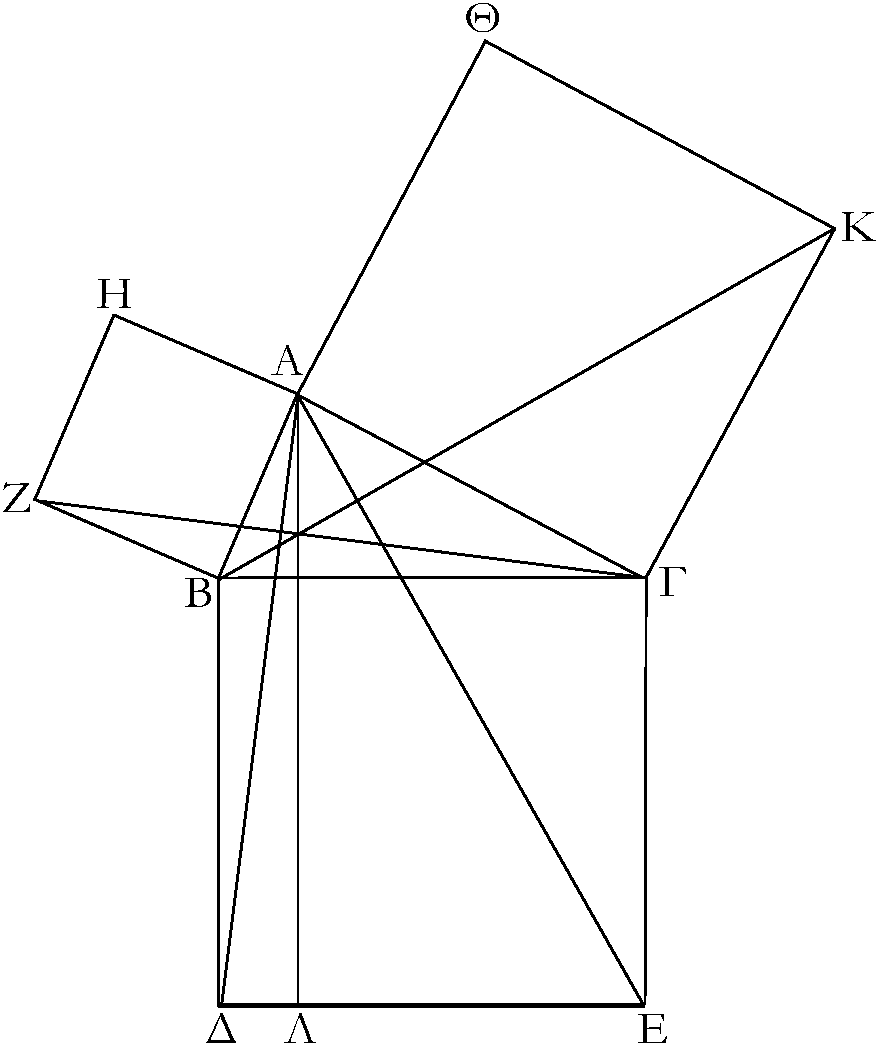
\includegraphics[width=0.8\textwidth]{Book01/fig47g.pdf}}

\gr{Ἀναγεγράφθω γὰρ ἀπὸ μὲν τῆς ΒΓ τετράγωνον τὸ ΒΔΕΓ, ἀπὸ δὲ τῶν ΒΑ, ΑΓ τὰ ΗΒ, ΘΓ, καὶ διὰ τοῦ Α ὁποτέρᾳ τῶν ΒΔ, ΓΕ παράλληλος ἢθθω ἡ ΑΛ; καὶ ἐπεζεύθθωσαν αἱ ΑΔ, ΖΓ. καὶ ἐπεὶ ὀρθή ἐστιν ἑκατέρα τῶν ὑπὸ ΒΑΓ, ΒΑΗ γωνιῶν, πρὸς δή τινι εὐθείᾳ τῇ ΒΑ καὶ τῷ πρὸς αὐτῇ σημείῳ τῷ Α δύο εὐθεῖαι αἱ ΑΓ, ΑΗ μὴ ἐπὶ τὰ αὐτὰ μέρη κείμεναι τὰξ ἐφεχῆς γωνίας δυσὶν ὀρθαῖξ ἴσας ποιοῦσιν; ἐπ' εὐθείας ἄρα ἐστὶν ἡ ΓΑ τῇ ΑΗ. διὰ τὰ αὐτὰ δὴ καὶ ἡ ΒΑ τῇ ΑΘ ἐστιν ἐπ' εὐθείας. καὶ ἐπεὶ ὸίση ἐστὶν ἡ ὑπὸ ΔΒΓ γωνία τῇ ὑπὸ ΖΒΑ; ὀρθὴ γὰρ ἑκατέρα; κοινὴ προσκείσθω ἡ ὑπὸ ΑΒΓ; ὅλη ἄρα ἡ ὑπὸ ΔΒΑ ὅλῃ τῇ ὑπὸ ΖΒΓ ἐστινὸίση.
καὶ ἐπεὶ ὸίση ἐστὶν ἡ μὲν ΔΒ τῇ ΒΓ, ἡ δὲ ΖΒ τῇ ΒΑ, δύο δὴ αἱ ΔΒ, ΒΑ δύο ταῖς ΖΒ, ΒΓ ἴσαι  εἰσὶν ἑκατέρα ἑκατέρᾳ;
καὶ γωνία ἡ ὑπὸ ΔΒΑ γωνίᾳ τῇ ὑπὸ ΖΒΓὸίση;
βάσις ἄρα ἡ ΑΔ βάσει τῇ ΖΓ [ἐστιν] ὸίση, καὶ τὸ ΑΒΔ τρίγωνον τῷ ΖΒΓ τριγώνῳ ἐστὶν ἴσον; καί [ἐστι] τοῦ μὲν ΑΒΔ τριγώνου διπλάσιον τὸ ΒΛ παραλληλόγραμμον; βάσιν τε γὰρ τὴν αὐτὴνὸέθουσι τὴν ΒΔ καὶ ἐν ταῖς αὐταῖς εἰσι παραλλήλοις ταῖς ΒΔ, ΑΛ; τοῦ δὲ ΖΒΓ τριγώνου διπλάσιον τὸ ΗΒ τετράγωνον; βάσιν τε γὰρ πάλιν τὴν αὐτὴνὸέθουσι τὴν ΖΒ καὶ ἐν ταῖς αὐταῖς εἰσι παραλλήλοις ταῖς ΖΒ, ΗΓ. [τὰ δὲ τῶνὸίσων διπλάσια ἴσα ἀλλήλοις ἐστίν;]  ἴσον ἄρα ἐστὶ καὶ τὸ ΒΛ παραλληλόγραμμον τῷ ΗΒ τετραγώνῳ. ὁμοίως δὴ ἐπιζευγνυμένων τῶν ΑΕ, ΒΚ δειθθήσεται καὶ τὸ ΓΛ παραλληλόγραμμον ἴσον τῷ ΘΓ τετραγώνῳ; ὅλον ἄρα τὸ ΒΔΕΓ τετράγωνον δυσὶ τοῖς ΗΒ, ΘΓ τετραγώνοις ἴσον ἐστίν. καί ἐστι τὸ μὲν ΒΔΕΓ τετράγωνον ἀπὸ τῆς ΒΓ ἀναγραφέν, τὰ δὲ ΗΒ, ΘΓ ἀπὸ τῶν ΒΑ, ΑΓ. τὸ  ἄρα ἀπὸ τῆς ΒΓ πλευρᾶξ τετράγωνον ἴσον ἐστὶ τοῖς ἀπὸ τῶν ΒΑ, ΑΓ
πλευρῶν τετραγώνοις.}

\gr{Ἐν ἄρα  τοῖς ὀρθογωνίοις τριγώνοις τὸ ἀπὸ τῆς τὴν ὀρθὴν γωνίαν ὑποτεινούσης πλευρᾶξ τετράγωνον ἴσον ἐστὶ τοῖς ἀπὸ τῶν τὴν ὀρθὴν [γωνίαν] περιεθουσῶν πλευρῶν τετραγώνοις; ὅπερ ἔδει δεῖχαι.}}

\ParallelRText{
\begin{center}
{\large Proposition 47}
\end{center}

In right-angled triangles,  the square on the side subtending the right-angle
is equal to the (sum of the) squares on the sides containing the right-angle.

Let $ABC$ be a right-angled triangle having the angle $BAC$ a right-angle. I say that the
square on $BC$ is equal to the (sum of the) squares on $BA$ and $AC$.

% Removed epsf size command
\centerline{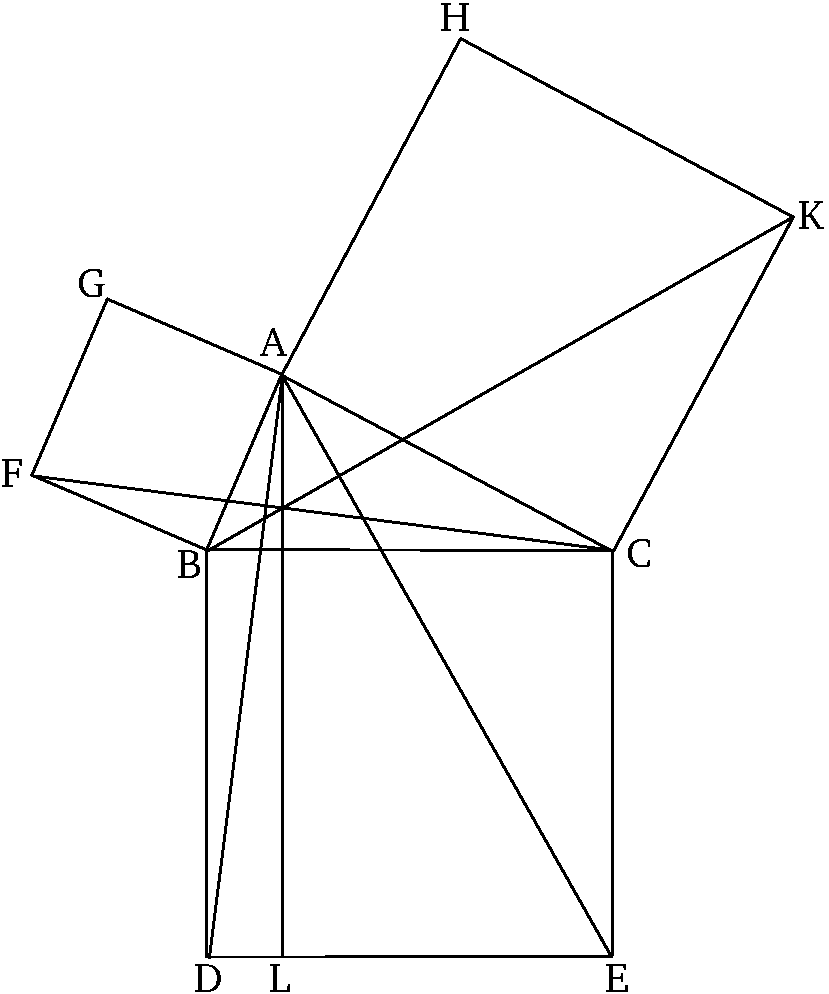
\includegraphics[width=0.8\textwidth]{Book01/fig47e.pdf}}

For let the square $BDEC$ be described on $BC$, and (the squares) $GB$ and $HC$ on $AB$ and $AC$ (respectively) [Prop.~1.46]. And let $AL$ be drawn through point $A$ parallel to either of $BD$ or $CE$ [Prop.~1.31]. And let $AD$ and $FC$ be joined. And
since angles $BAC$ and $BAG$ are each right-angles, then two straight-lines $AC$ and $AG$, not lying on the same side,
make the adjacent angles with some straight-line $BA$, at the point
$A$ on it, (whose sum is) equal to two right-angles. Thus, $CA$ is straight-on to $AG$ [Prop.~1.14]. So, for
the same (reasons), $BA$ is also straight-on to $AH$. And since angle $DBC$ is
equal to $FBA$, for (they are) both right-angles, let $ABC$ be added to
both.  Thus, the whole (angle) $DBA$ is equal to the whole (angle) $FBC$.
And since $DB$ is equal to $BC$, and $FB$ to $BA$, the two (straight-lines) $DB$,
$BA$ are equal to the two (straight-lines) $CB$, $BF$,$^\dag$ respectively. And angle $DBA$ (is) equal to angle $FBC$. Thus, the base $AD$ [is] equal to the base $FC$,
and the triangle $ABD$ is equal to the triangle $FBC$ [Prop.~1.4]. And 
parallelogram $BL$ [is] double (the area) of triangle $ABD$. For they
have the same base, $BD$, and are between the same parallels, $BD$ and $AL$  [Prop.~1.41]. And
 square
$GB$ is double (the area) of triangle $FBC$. For again they have the same base, $FB$, and
are between the same parallels,
$FB$ and $GC$ [Prop.~1.41]. [And the doubles of equal things
are equal to one another.]$^\ddag$ Thus, the parallelogram $BL$ is also equal to the square $GB$. So, similarly, $AE$ and $BK$ being joined, 
the parallelogram $CL$ can be shown (to be)  equal to the square $HC$. Thus, the whole square
$BDEC$ is equal to the (sum of the) two squares $GB$ and $HC$. And the square $BDEC$
is described on $BC$, and the (squares) $GB$ and $HC$ on $BA$ and $AC$ (respectively). Thus, the square on the side $BC$ is equal to the
(sum of the) squares
on the sides $BA$ and $AC$.

Thus, in right-angled triangles,  the square on the side subtending the right-angle
is equal to the (sum of the) squares on the sides surrounding the right-[angle].
(Which is) the very thing it was required to show.}
\end{Parallel}
{\footnotesize \noindent$^\dag$ The
Greek text has ``$FB$, $BC$'', which is obviously a mistake.\\[0.5ex]
$^\ddag$ This is an additional common notion.}

%%%%%%
% Prop 1.48
%%%%%%
\pdfbookmark[1]{Proposition 1.48}{pdf1.48}
\begin{Parallel}{}{} 
\ParallelLText{
\begin{center}
{\large\ggn{48}.}
\end{center}\vspace*{-7pt}

\gr{Ἐὰν τριγώνου τὸ ἀπὸ μιᾶς τῶν πλευρῶν τετράγωνον ἴσονὸῆ| τοῖς ἀπὸ τῶν λοιπῶν τοῦ τριγώνου δύο πλευρῶν τετραγώνοις, ἡ περιεθομένη γωνία ὑπὸ τῶν λοιπῶν τοῦ τριγώνου δύο πλευρῶν ὀρθή ἐστιν.}

\gr{Τριγώνου γὰρ τοῦ ΑΒΓ τὸ ἀπὸ μιᾶς τῆς ΒΓ πλευρᾶξ τετράγωνον ἴσονὸέστω τοῖς ἀπὸ τῶν ΒΑ, ΑΓ πλευρῶν τετραγώνοις; λέγω, ὅτι ὀρθή ἐστιν ἡ ὑπὸ ΒΑΓ γωνία.}

% Removed epsf size command
\centerline{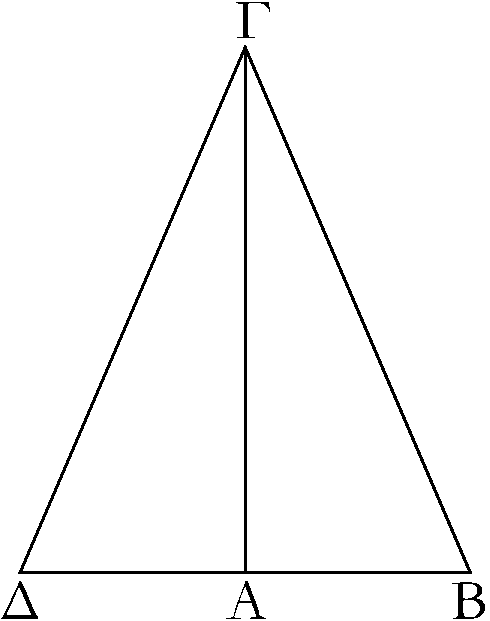
\includegraphics[width=0.8\textwidth]{Book01/fig48g.pdf}}

\gr{ὸ'Ηθθω γὰρ ἀπὸ τοῦ Α σημείου τῇ ΑΓ εὐθείᾳ πρὸς ὀρθὰξ ἡ ΑΔ καὶ κείσθω τῇ ΒΑὸίση ἡ ΑΔ, καὶ ἐπεζεύθθω ἡ ΔΓ. ἐπεὶ ὸίση
ἐστὶν ἡ ΔΑ τῇ ΑΒ,  ἴσον ἐστὶ καὶ τὸ ἀπὸ τῆς ΔΑ τετράγωνον τῷ ἀπὸ τῆς ΑΒ τετραγώνῳ. κοινὸν προσκείσθω τὸ ἀπὸ τῆς ΑΓ τετράγωνον; τὰ  ἄρα ἀπὸ τῶν ΔΑ, ΑΓ τετράγωνα ἴσα ἐστὶ τοῖς ἀπὸ τῶν ΒΑ, ΑΓ τετραγώνοις. ἀλλὰ τοῖς μὲν ἀπὸ τῶν ΔΑ, ΑΓ ἴσον ἐστὶ τὸ ἀπὸ τῆς ΔΓ; ὀρθὴ γάρ ἐστιν ἡ ὑπὸ ΔΑΓ γωνία; τοῖς δὲ ἀπὸ τῶν ΒΑ, ΑΓ ἴσον ἐστὶ τὸ ἀπὸ τῆς ΒΓ; ὑπόκειται γάρ; τὸ  ἄρα ἀπὸ τῆς ΔΓ τετράγωνον ἴσον ἐστὶ τῷ ἀπὸ τῆς ΒΓ τετραγώνῳ; ὁώστε καὶ πλευρὰ ἡ ΔΓ τῇ ΒΓ ἐστινὸίση; καὶ ἐπεὶ ὸίση ἐστὶν ἡ ΔΑ τῇ ΑΒ, κοινὴ δὲ ἡ ΑΓ, δύο δὴ αἱ ΔΑ, ΑΓ δύο ταῖς ΒΑ, ΑΓ ἴσαι εἰσίν; καὶ βάσις ἡ ΔΓ βάσει τῇ ΒΓὸίση; γωνία ἄρα ἡ ὑπὸ ΔΑΓ γωνίᾳ τῇ ὑπὸ ΒΑΓ [ἐστιν] ὸίση. ὀρθὴ δὲ ἡ ὑπὸ ΔΑΓ; ὀρθὴ  ἄρα καὶ ἡ ὑπὸ ΒΑΓ.}

\gr{Ἐὰν ἀρὰ τριγώνου τὸ ἀπὸ μιᾶς τῶν πλευρῶν τετράγωνον ἴσονὸῆ| τοῖς ἀπὸ τῶν λοιπῶν τοῦ τριγώνου δύο πλευρῶν τετραγώνοις, ἡ περιεθομένη γωνία ὑπὸ τῶν λοιπῶν τοῦ τριγώνου δύο πλευρῶν ὀρθή ἐστιν; ὅπερ ἔδει δεῖχαι.}}

\ParallelRText{
\begin{center}
{\large Proposition 48}
\end{center}

If the square on one of the sides of a triangle is equal to the (sum of the)
squares on the two remaining sides of the triangle (then) the angle contained
by the two remaining sides of the triangle is a right-angle.

For let the square on one of the sides, $BC$, of triangle $ABC$ be equal
to the (sum of the) squares on the sides $BA$ and $AC$. I say that angle
$BAC$ is a right-angle.

% Removed epsf size command
\centerline{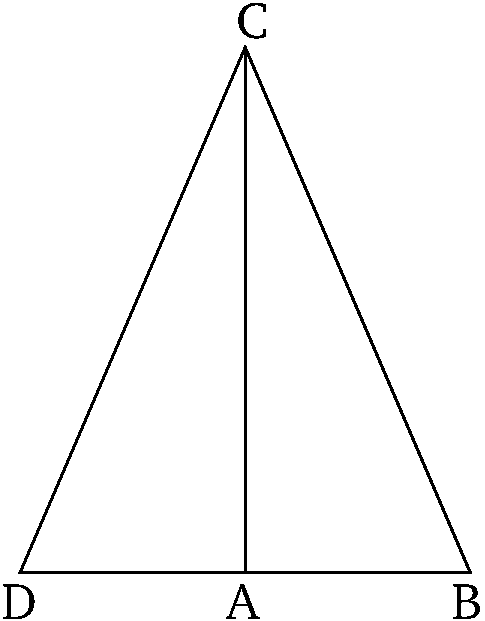
\includegraphics[width=0.8\textwidth]{Book01/fig48e.pdf}}

For let $AD$ be drawn from point $A$ at right-angles to the
straight-line $AC$ [Prop.~1.11], and let $AD$ be made equal to
$BA$ [Prop.~1.3], and let $DC$ be joined. Since $DA$ is equal to $AB$,
the square on $DA$ is thus also equal to the square on $AB$.$^\dag$ Let the square on
$AC$ be added to both. Thus, the (sum of the) squares on $DA$ and $AC$ is equal
to the (sum of the) squares on $BA$ and $AC$. But, the (square) on $DC$ 
is equal to the (sum of the squares) on $DA$ and $AC$. For angle $DAC$ is a right-angle [Prop.~1.47].
But, the  (square) on $BC$ is equal to (sum of the squares) on $BA$ and $AC$.
For (that) was assumed. Thus, the square on $DC$ is equal to the square on $BC$.
So  side $DC$ is also equal to (side) $BC$. And since $DA$ is equal to $AB$, and $AC$ (is) common, the two (straight-lines) $DA$, $AC$ are equal to the two (straight-lines)
$BA$, $AC$. And the base $DC$ is equal to the base $BC$. Thus, angle $DAC$ [is] equal to angle $BAC$ [Prop.~1.8].  But $DAC$ is a right-angle. Thus, $BAC$ is
also a right-angle.

Thus, if the square on one of the sides of a triangle is equal to the (sum of the)
squares on the remaining two sides of the triangle (then) the angle contained
by the remaining two sides of the triangle is a right-angle. (Which is) the very thing
it was required to show.}
\end{Parallel}
{\footnotesize \noindent$^\dag$ Here, use is made of the additional common notion that the squares of equal things are
themselves equal. Later on, the inverse notion is used.} 